% Options for packages loaded elsewhere
\PassOptionsToPackage{unicode}{hyperref}
\PassOptionsToPackage{hyphens}{url}
%
\documentclass[UTF8]{article}
\usepackage{amsmath,amssymb}
\usepackage{iftex}
\usepackage{CTEX}
\usepackage[backend=bibtex]{biblatex}
\ifPDFTeX
  \usepackage[T1]{fontenc}
  \usepackage[utf8]{inputenc}
  \usepackage{textcomp} % provide euro and other symbols
\else % if luatex or xetex
  \usepackage{unicode-math} % this also loads fontspec
  \defaultfontfeatures{Scale=MatchLowercase}
  \defaultfontfeatures[\rmfamily]{Ligatures=TeX,Scale=1}
\fi
\usepackage{lmodern}
\ifPDFTeX\else
  % xetex/luatex font selection
\fi
% Use upquote if available, for straight quotes in verbatim environments
\IfFileExists{upquote.sty}{\usepackage{upquote}}{}
\IfFileExists{microtype.sty}{% use microtype if available
  \usepackage[]{microtype}
  \UseMicrotypeSet[protrusion]{basicmath} % disable protrusion for tt fonts
}{}
\makeatletter
\@ifundefined{KOMAClassName}{% if non-KOMA class
  \IfFileExists{parskip.sty}{%
    \usepackage{parskip}
  }{% else
    \setlength{\parindent}{0pt}
    \setlength{\parskip}{6pt plus 2pt minus 1pt}}
}{% if KOMA class
  \KOMAoptions{parskip=half}}
\makeatother
\usepackage{xcolor}
\usepackage{graphicx}
\makeatletter
\def\maxwidth{\ifdim\Gin@nat@width>\linewidth\linewidth\else\Gin@nat@width\fi}
\def\maxheight{\ifdim\Gin@nat@height>\textheight\textheight\else\Gin@nat@height\fi}
\makeatother
% Scale images if necessary, so that they will not overflow the page
% margins by default, and it is still possible to overwrite the defaults
% using explicit options in \includegraphics[width, height, ...]{}
\setkeys{Gin}{width=\maxwidth,height=\maxheight,keepaspectratio}
% Set default figure placement to htbp
\makeatletter
\def\fps@figure{htbp}
\makeatother
\setlength{\emergencystretch}{3em} % prevent overfull lines
\providecommand{\tightlist}{%
  \setlength{\itemsep}{0pt}\setlength{\parskip}{0pt}}
\setcounter{secnumdepth}{-\maxdimen} % remove section numbering
\ifLuaTeX
  \usepackage{selnolig}  % disable illegal ligatures
\fi
\IfFileExists{bookmark.sty}{\usepackage{bookmark}}{\usepackage{hyperref}}
\IfFileExists{xurl.sty}{\usepackage{xurl}}{} % add URL line breaks if available
\urlstyle{same}
\hypersetup{
  hidelinks,
  pdfcreator={LaTeX via pandoc}}

\author{}
\date{}

\begin{document}

\section{第三章
不涉及圆的任意点作图}


\subsection{1. 基本定理}

\hypertarget{zykux57faux672cux5bf9ux79f0ux5b9aux7406}{%
\subsubsection{Zyk基本对称定理}\label{zykux57faux672cux5bf9ux79f0ux5b9aux7406}}

在 2022
年春季,Zyk同学受到B站视频BV16u411i75M的启发,提出了Zyk基本对称定理,内容如下:

\hypertarget{zykux57faux672cux5bf9ux79f0ux5b9aux7406-zyks-basic-symmetry-theorem-ux5b9aux7406-3.1}{%
\subsection{Zyk基本对称定理 Zyk's Basic Symmetry Theorem (定理
3.1)}\label{zykux57faux672cux5bf9ux79f0ux5b9aux7406-zyks-basic-symmetry-theorem-ux5b9aux7406-3.1}}

\textbf{【提出者】}翟悦凯

可以做出任意一点关于一条垂直格线或一条水平格线的对称点。做法如下(做
\(A\) 关于 \(l\) 的对称):

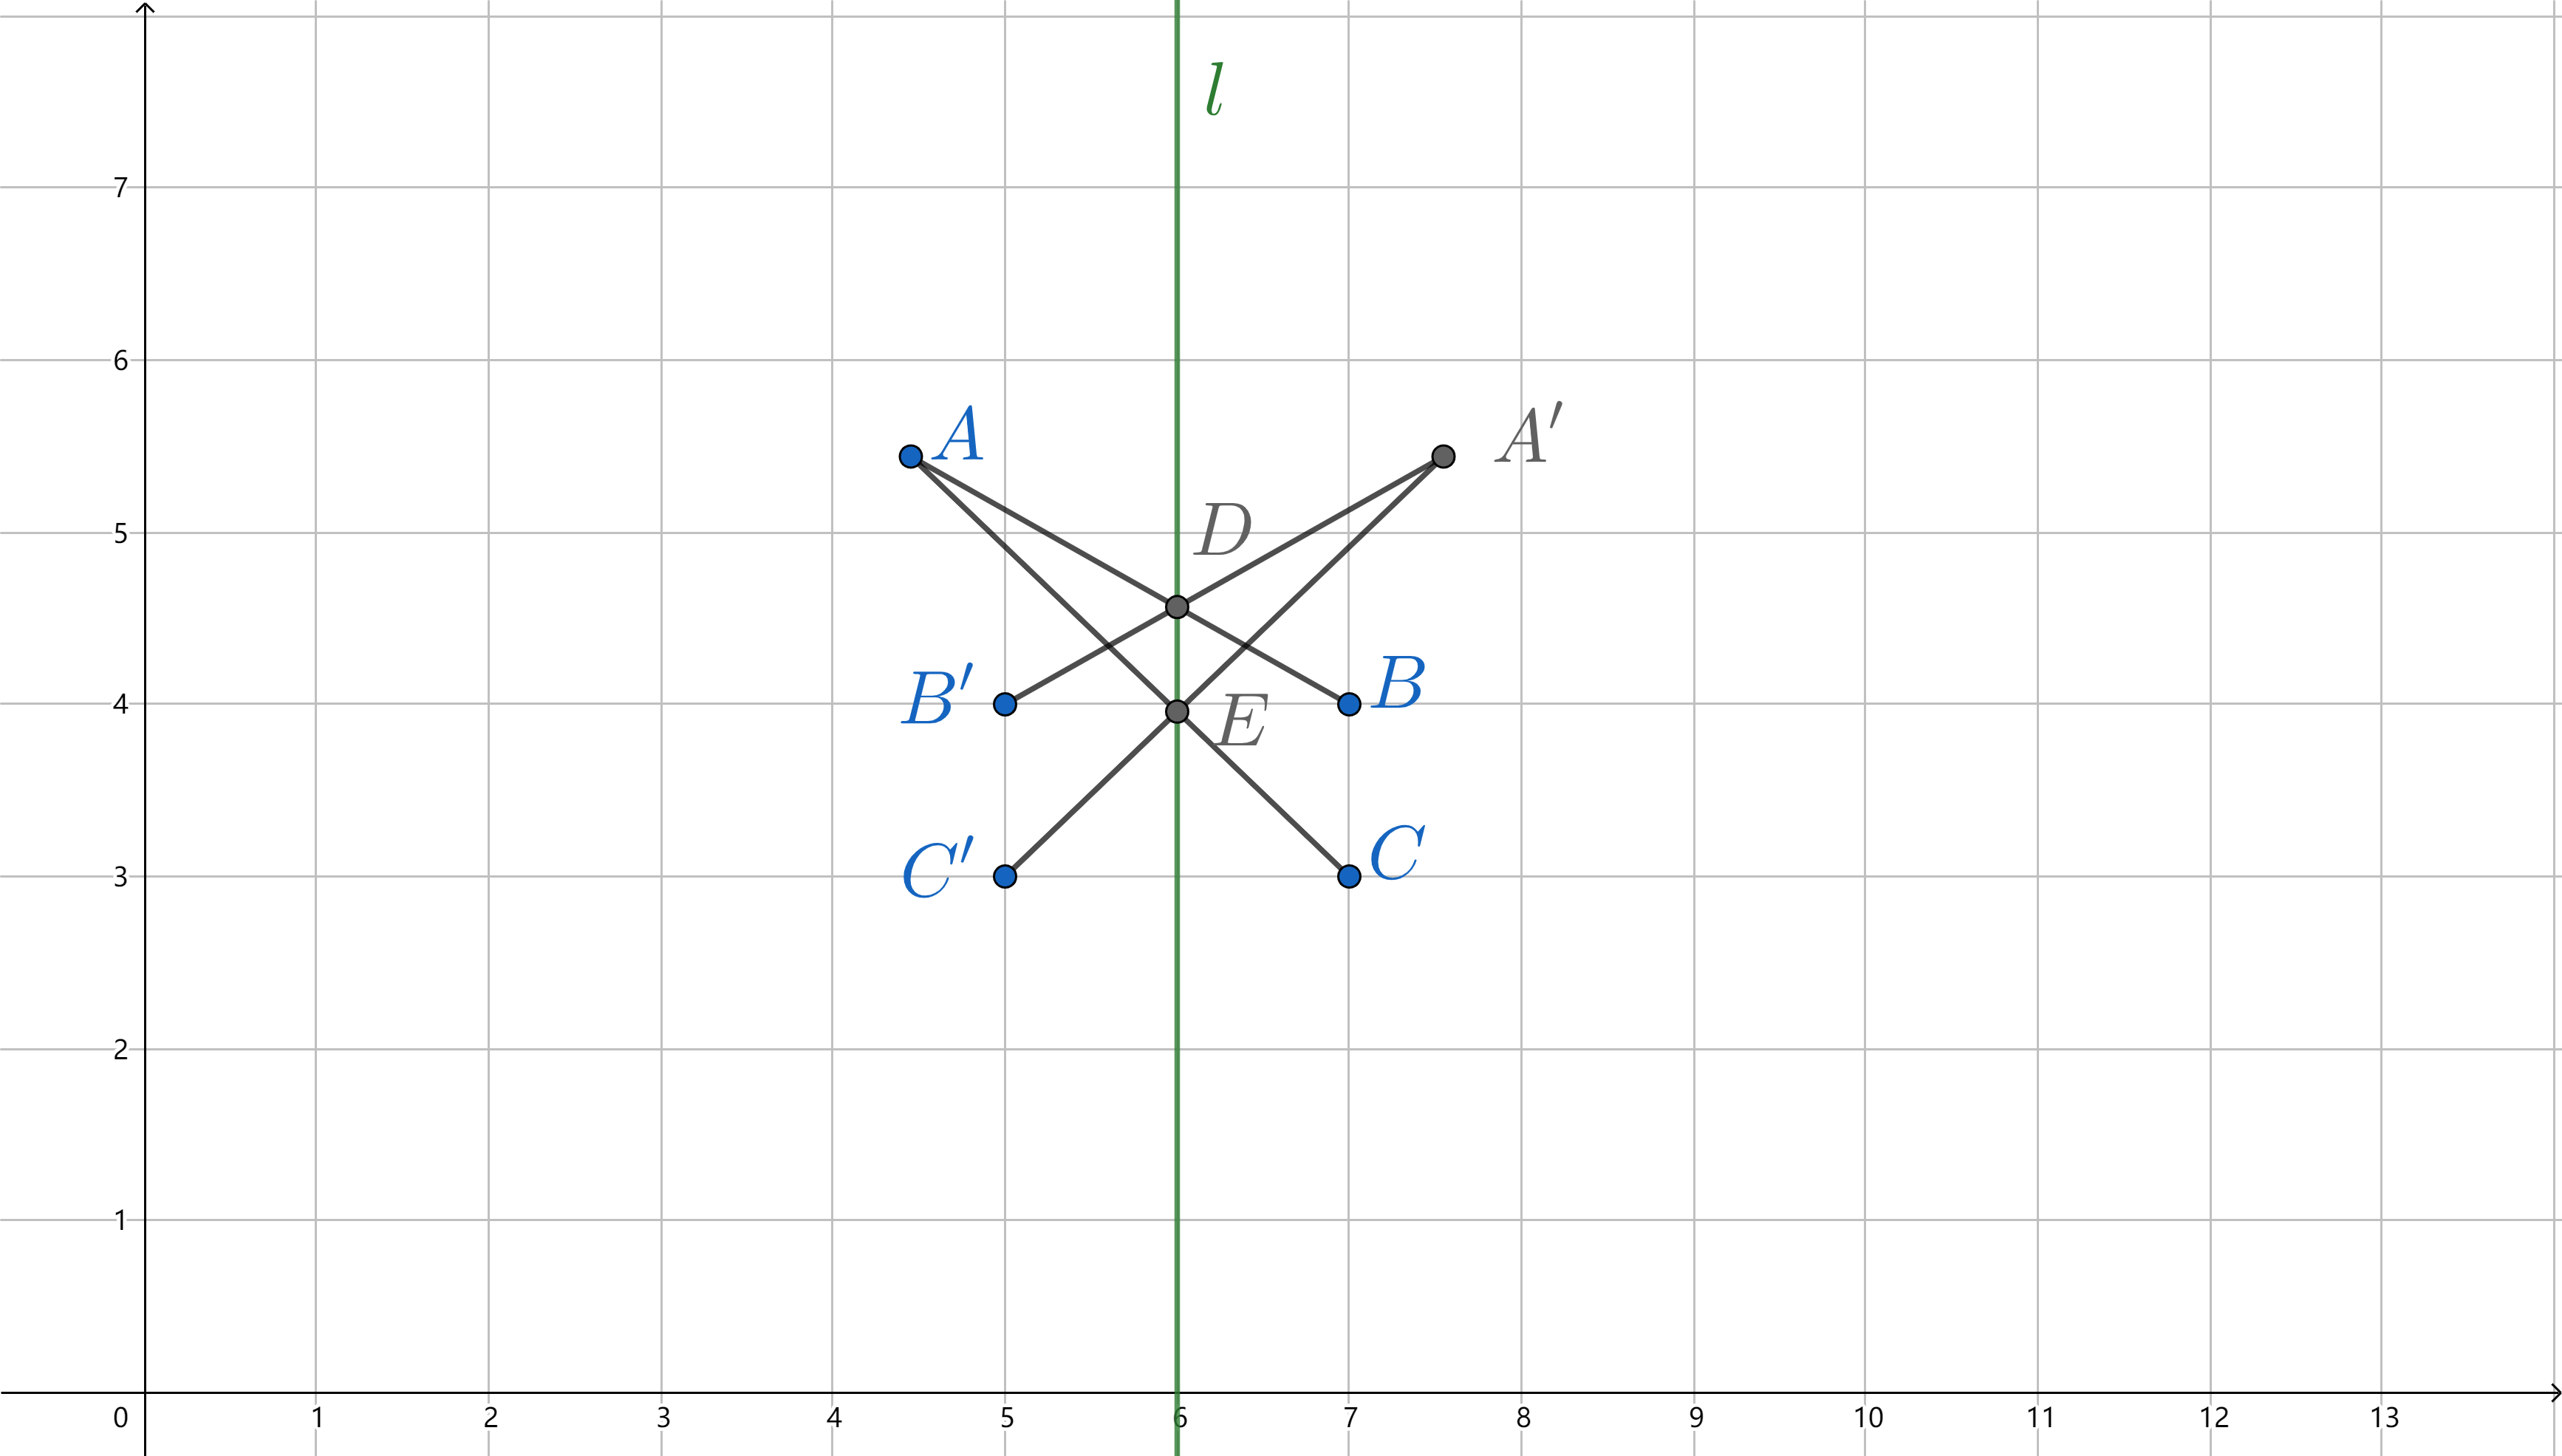
\includegraphics[width=5.76806in,height=3.27847in]{media/image1.png}

\textbf{【作图语句】}取格点 \(B,C,B^{'},C^{'}\)(要求 \(B^{'},C^{'}\)
关于 \(l\) 对称),连接 \(AB,\ AC\) 交 \(l\) 于 \(D,E\)。连
\(B^{'}D,C^{'}E\) 交于 \(A^{'}\)。\(A^{'}\) 即为所求。

\textbf{【拓展】}当 \(l\) 为网格中线时,此定理依然适用:

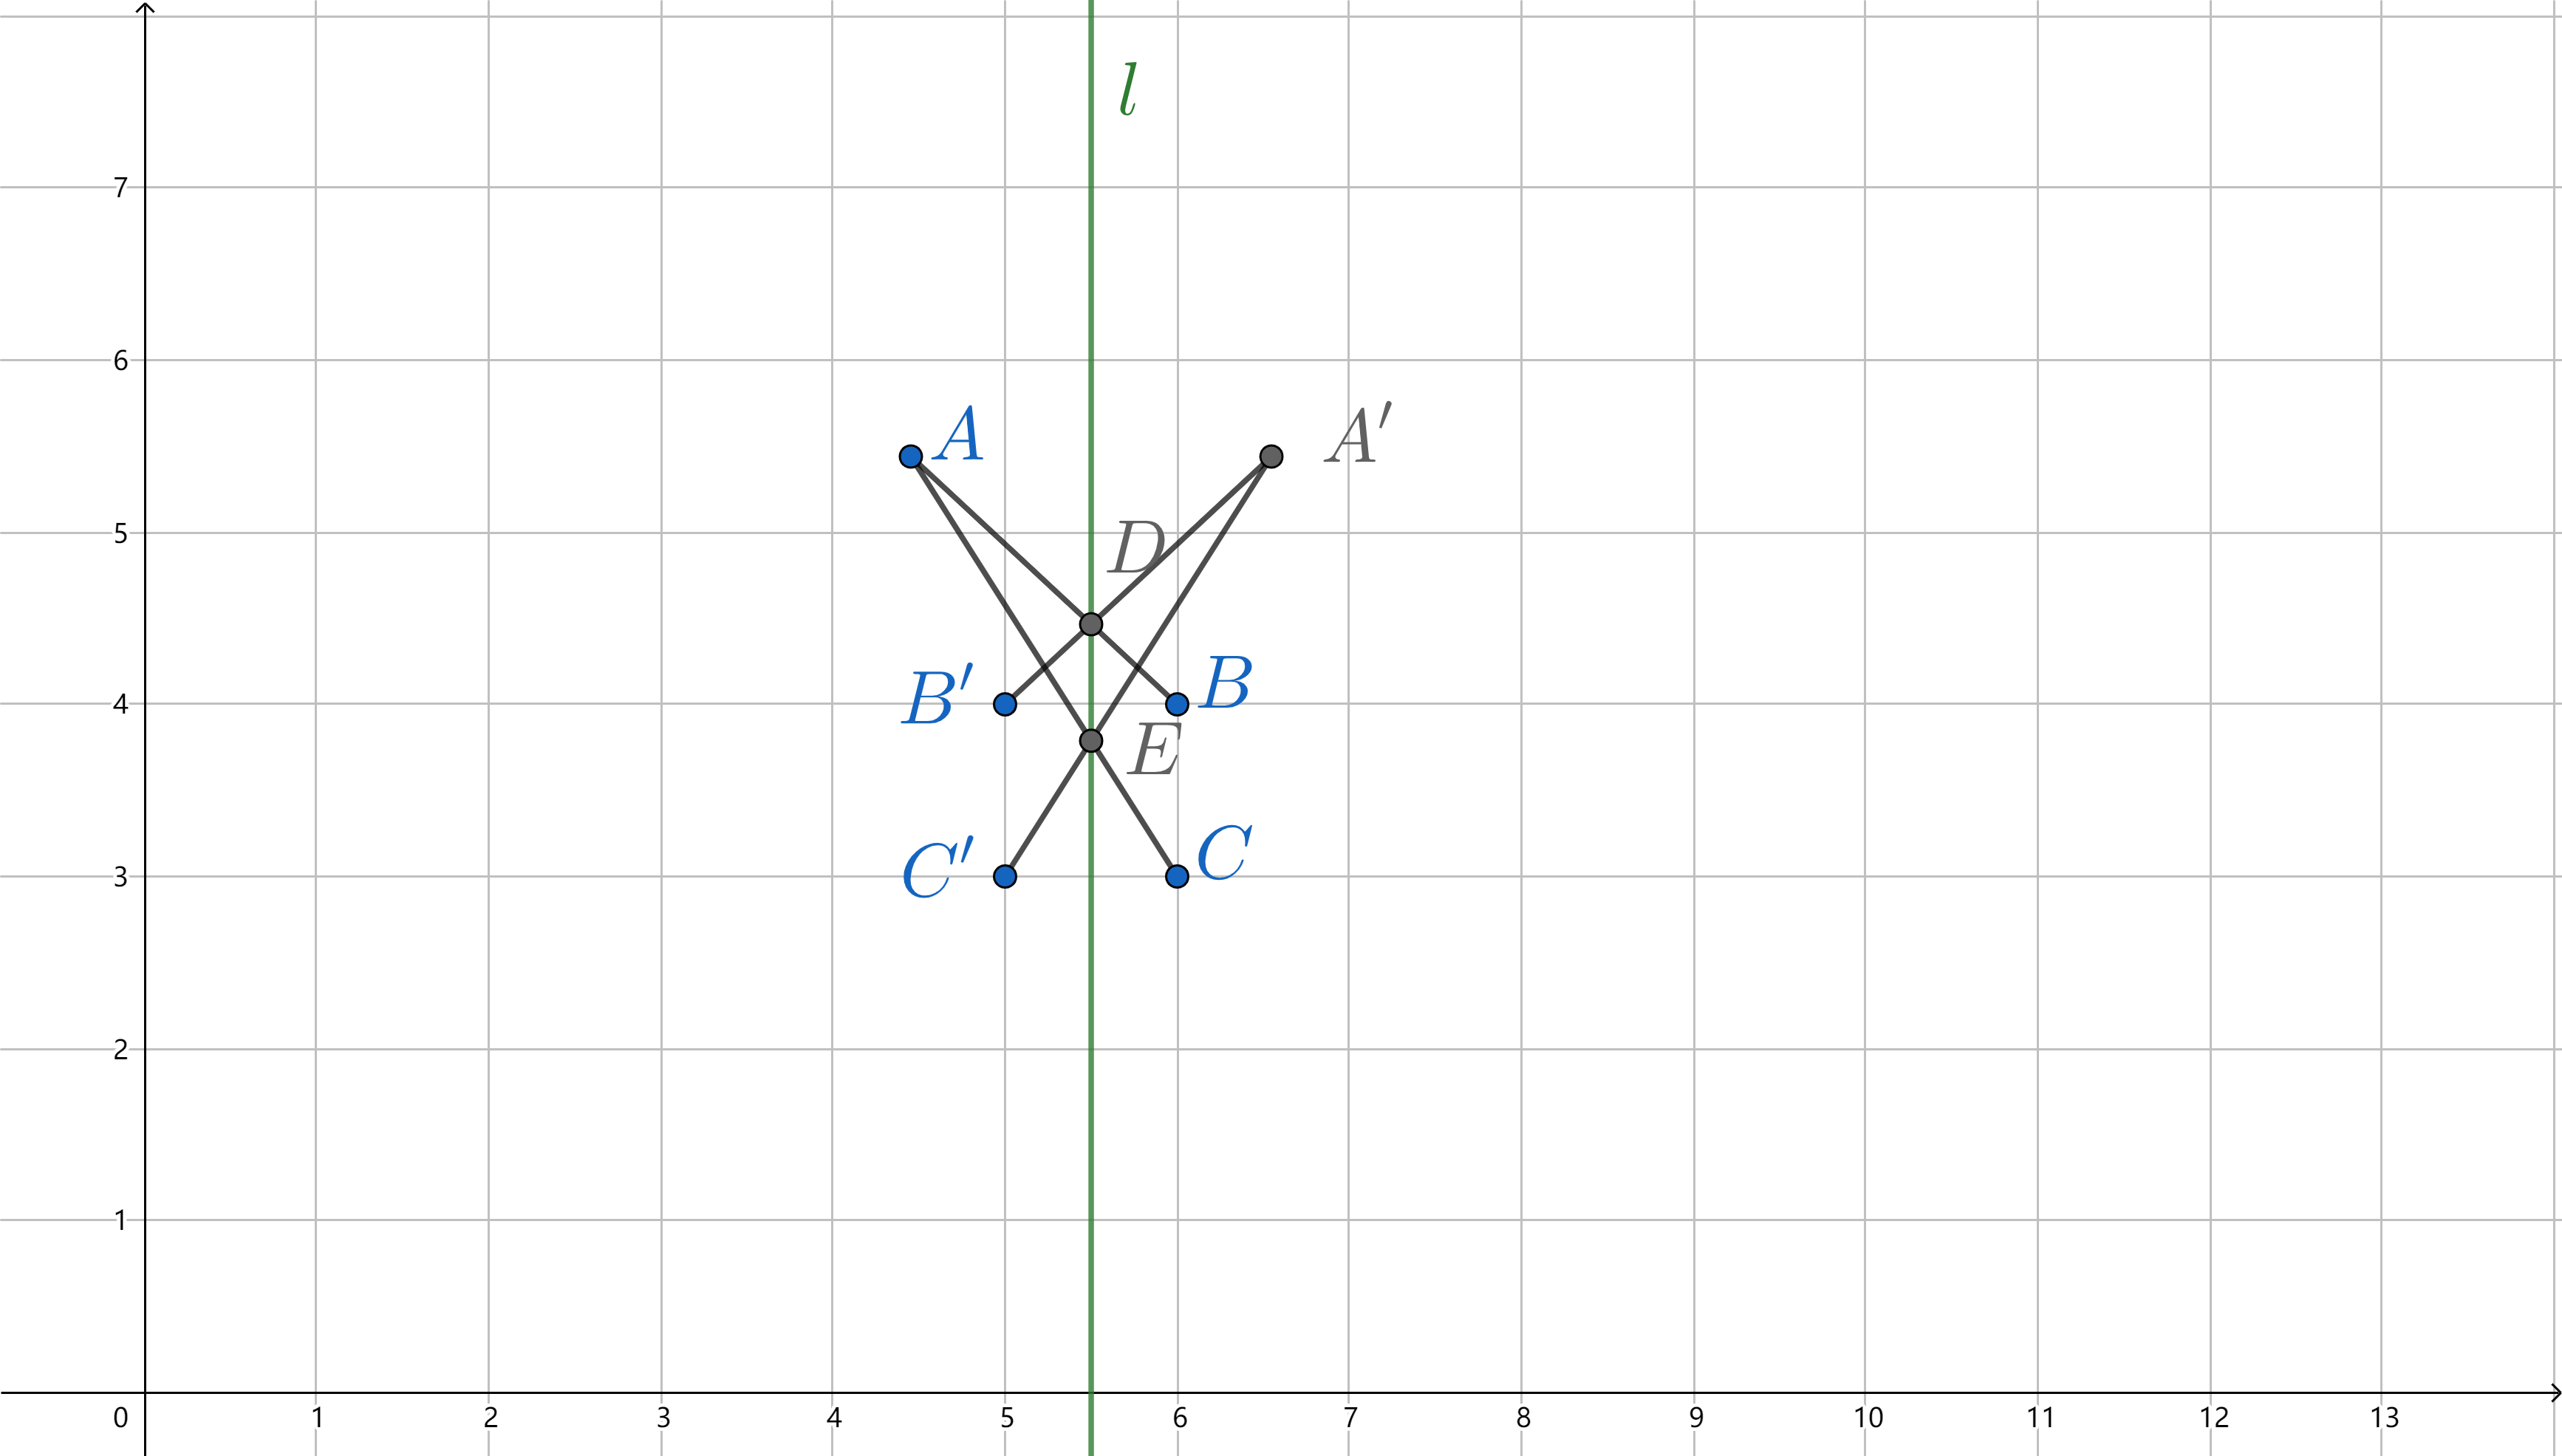
\includegraphics[width=5.76806in,height=3.27847in]{media/image2.png}

\textbf{【证明】}不难发现直线 \(AB\) 和直线 \(A^{'}B^{'}\) 对称,直线
\(AC\) 与直线 \(A^{'}C^{'}\) 对称,所以直线的交点也对称,这样 \(A\) 和
\(A^{'}\) 就是对称的了。

\textbf{【拓展】}这个定理用了两对对称点以确定 \(A^{'}\)
的位置,但在一些特殊情况下(比如 \(A\) 在水平格线上而 \(l\)
为竖直直线时),我们只需要一对对称点。下面的图片展示了一个例子。\(A\)
在水平格线上,我们不难看出 \(A^{'}\)
也在相同的水平格线上,于是可以省去一对对称点。

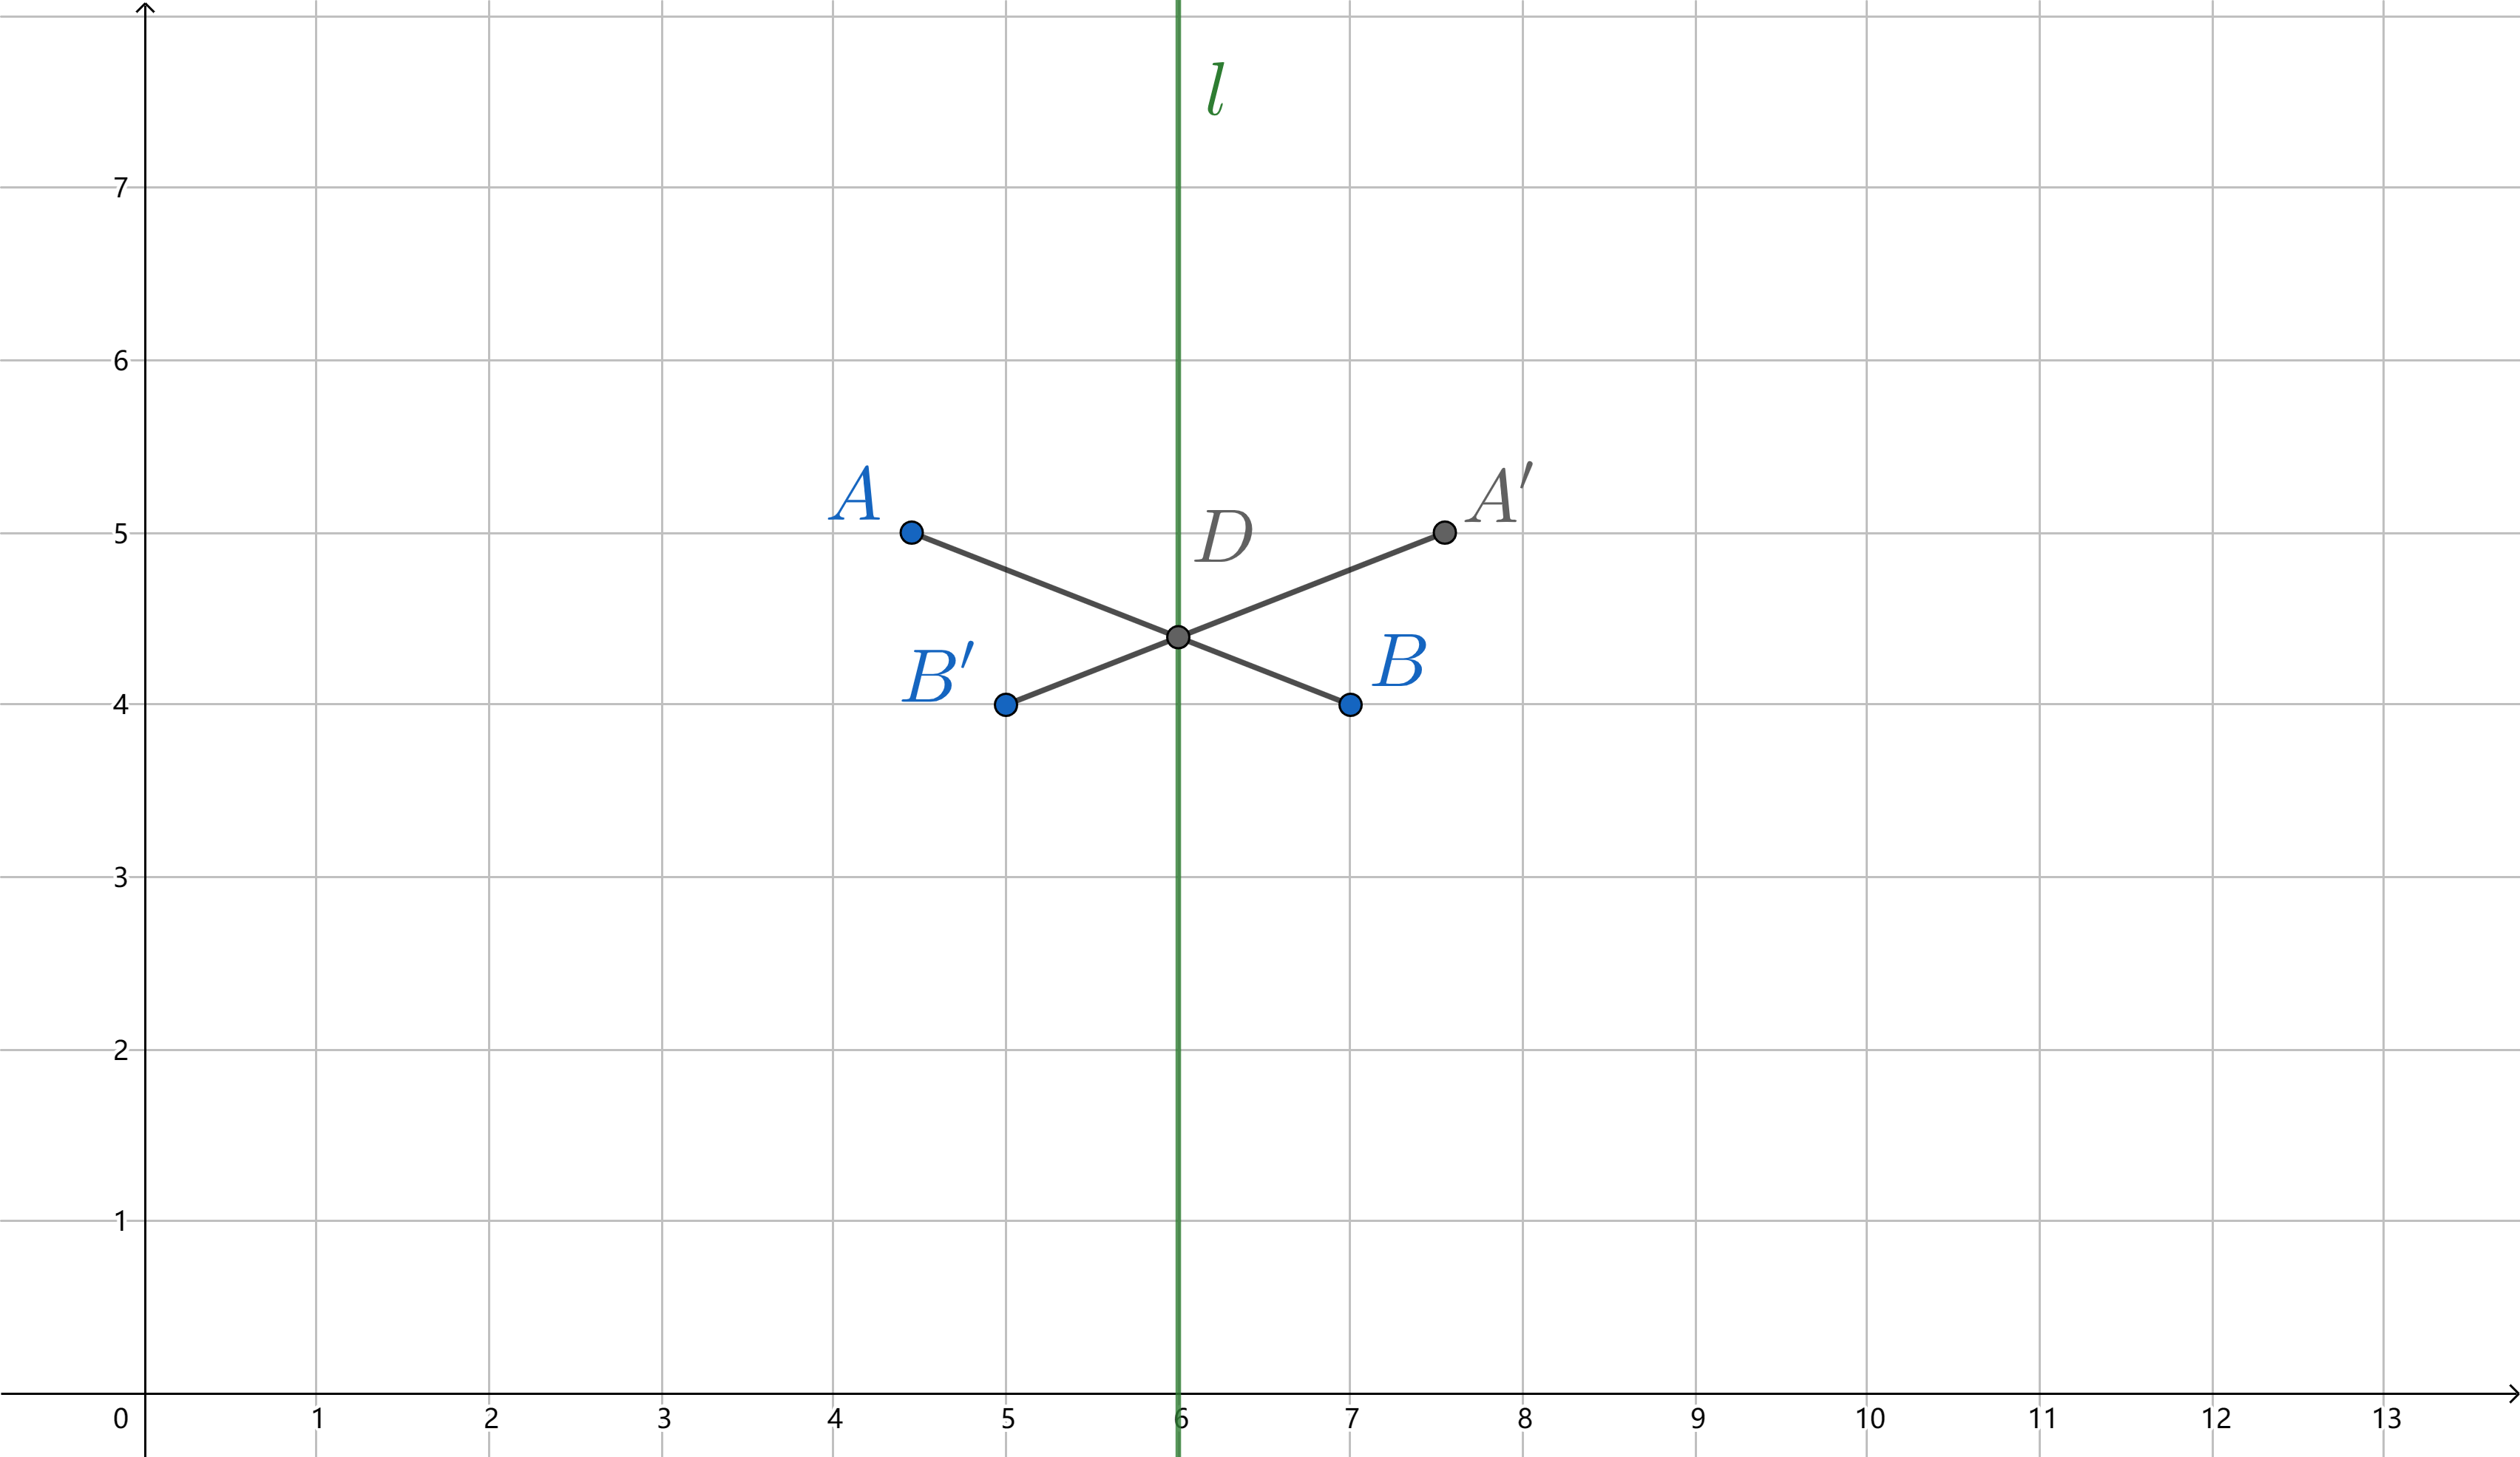
\includegraphics[width=5.76806in,height=3.33611in]{media/image3.png}

\textbf{【拓展】}当 \(l\) 为从网格对角线的时候,此定理依然适用。

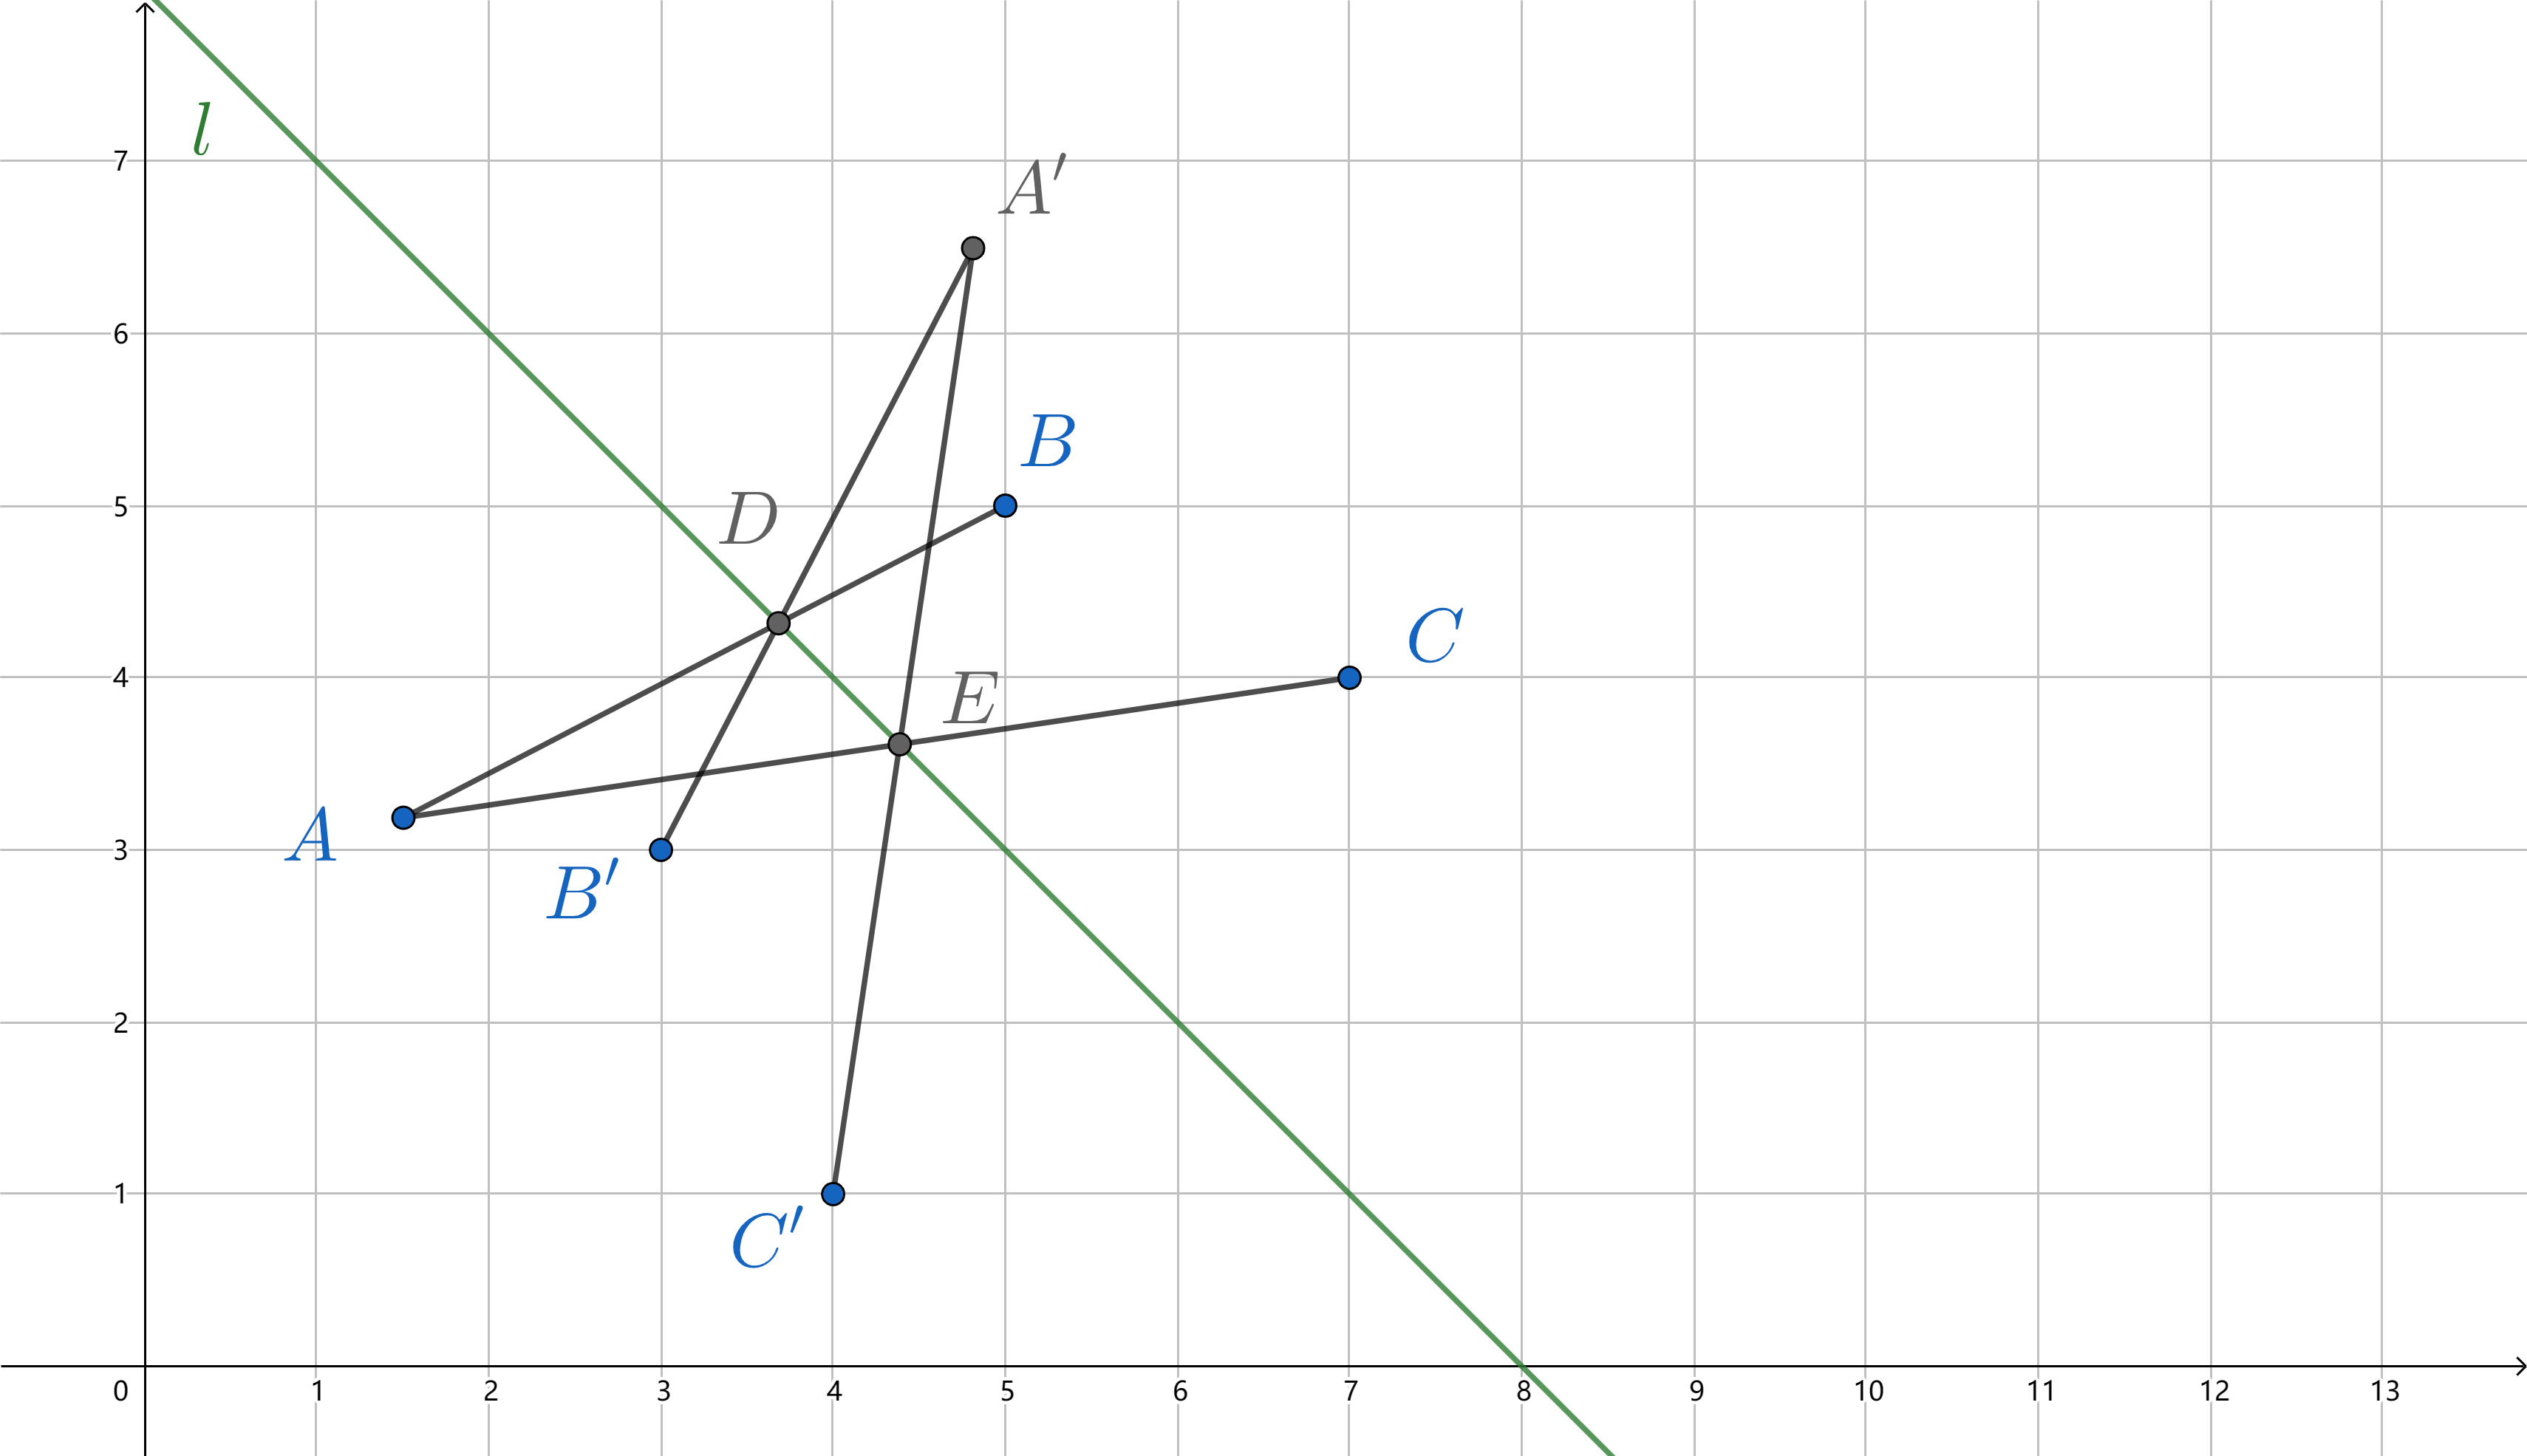
\includegraphics[width=5.76806in,height=3.32431in]{media/image4.png}

Zyk基本对称定理的一大优势是,可以做出任意点关于一条格线(或网格中线、网格对角线)的对称。\(B\),\(C\)
点的选择也比较自由,画图者可以通过选择合适的 \(B\),\(C\)
使得画图结果更美观。Zyk基本定理有非常多的推论,它们的原理都不难理解。我们来一一列举。

\hypertarget{ux63a8ux8bbaux5e73ux79fbux5b9aux7406-translate-theorem-ux5b9aux7406-3.1.1}{%
\subsection{推论:平移定理 Translate Theorem (定理
3.1.1)}\label{ux63a8ux8bbaux5e73ux79fbux5b9aux7406-translate-theorem-ux5b9aux7406-3.1.1}}

可以将任意点向左/向右/向上/向下平移 \(n\ \left( n \in N^{*} \right)\)
个单位长度。做法如下(将 \(A\) 向右平移):

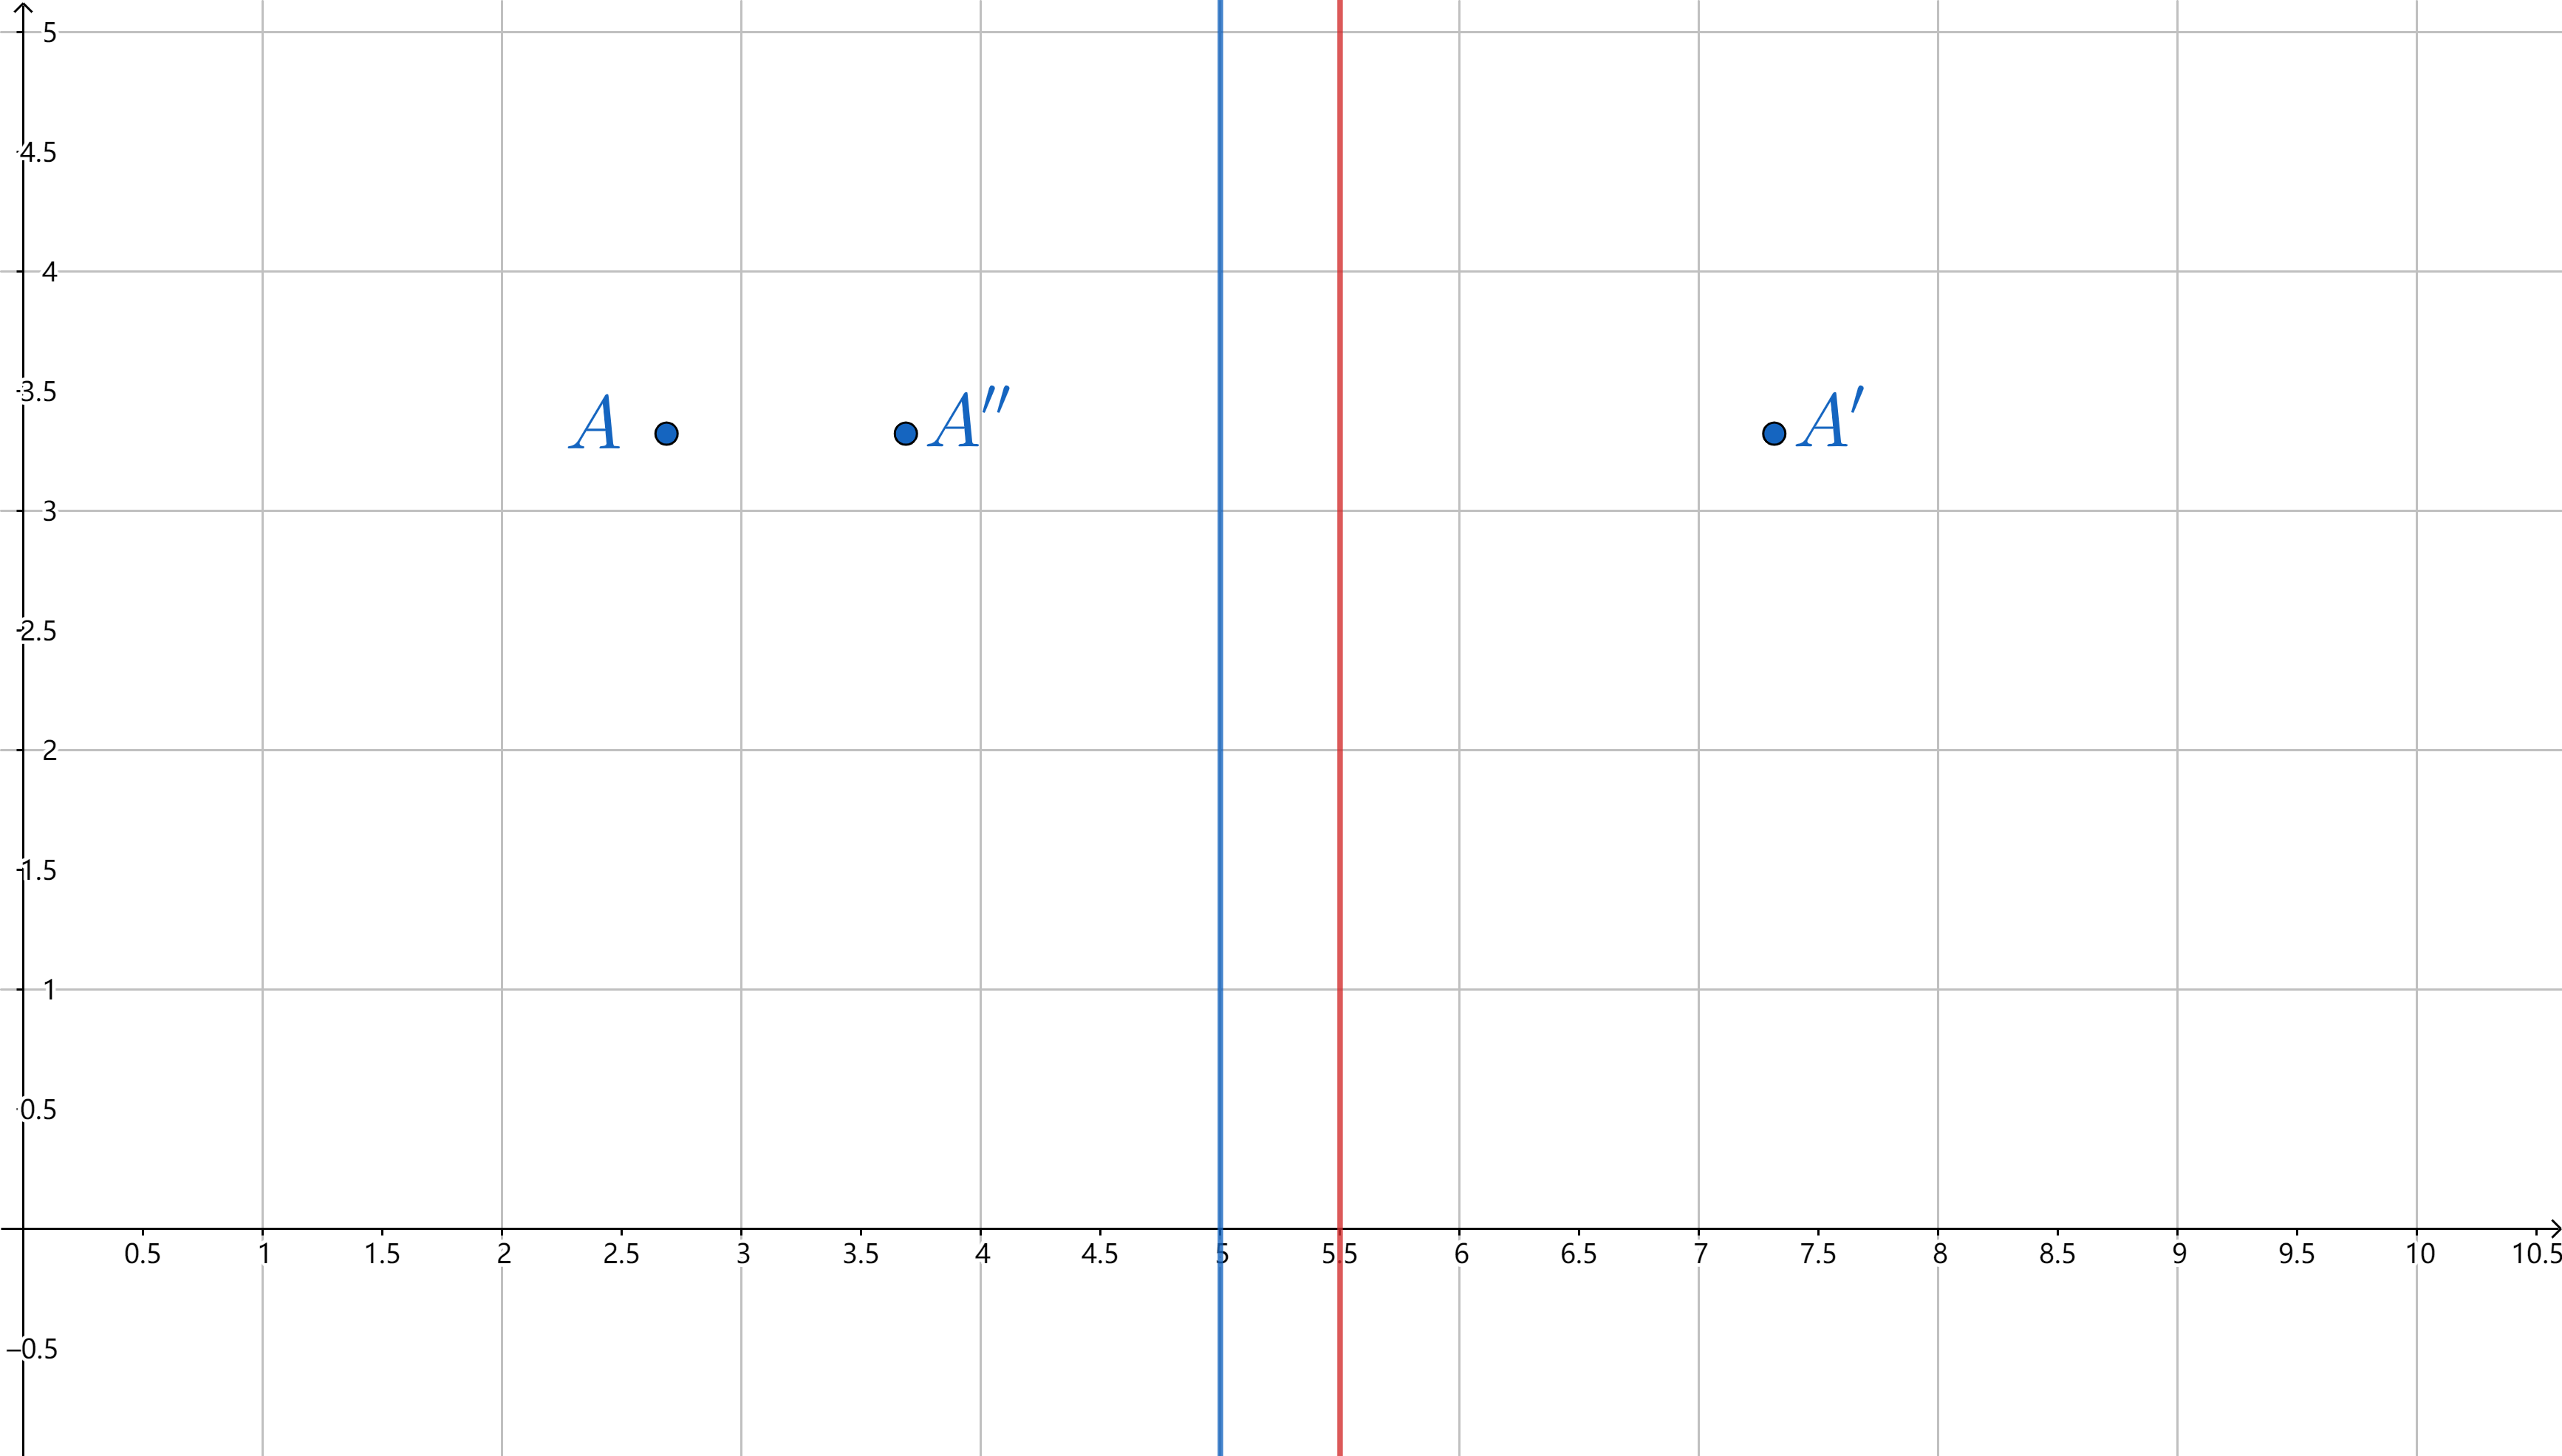
\includegraphics[width=5.76806in,height=3.27847in]{media/image5.png}我们以向右平移为例。选定一条格线,做点
\(A\) 关于这条直线的对称点 \(A^{'}\)。将选定直线向右平移 \(\frac{n}{2}\)
个单位(这通常是简单的),做 \(A^{'}\) 关于新直线的对称点
\(A^{''}\)。\(A^{''}\) 即为所求。

\textbf{【证明】}如果 \(A\) 与左边的直线相距 \(d\),那么
\(AA^{'} = 2d\),\(A^{'}\) 与右边的直线相距
\(d - 0.5n\),\(A^{'}A^{''} = 2d - n\)。所以 \(AA^{''} = n\)。

\hypertarget{ux63a8ux8bbaux5206ux7ebfux6bb5ux5b9aux7406-segment-dividing-theoremux5b9aux7406-3.1.2}{%
\subsection{推论:分线段定理 Segment Dividing Theorem(定理
3.1.2)}\label{ux63a8ux8bbaux5206ux7ebfux6bb5ux5b9aux7406-segment-dividing-theoremux5b9aux7406-3.1.2}}

可以把任意一条线段分成给定比例。作图方法如下(以平分线段 \(AB\) 为例):

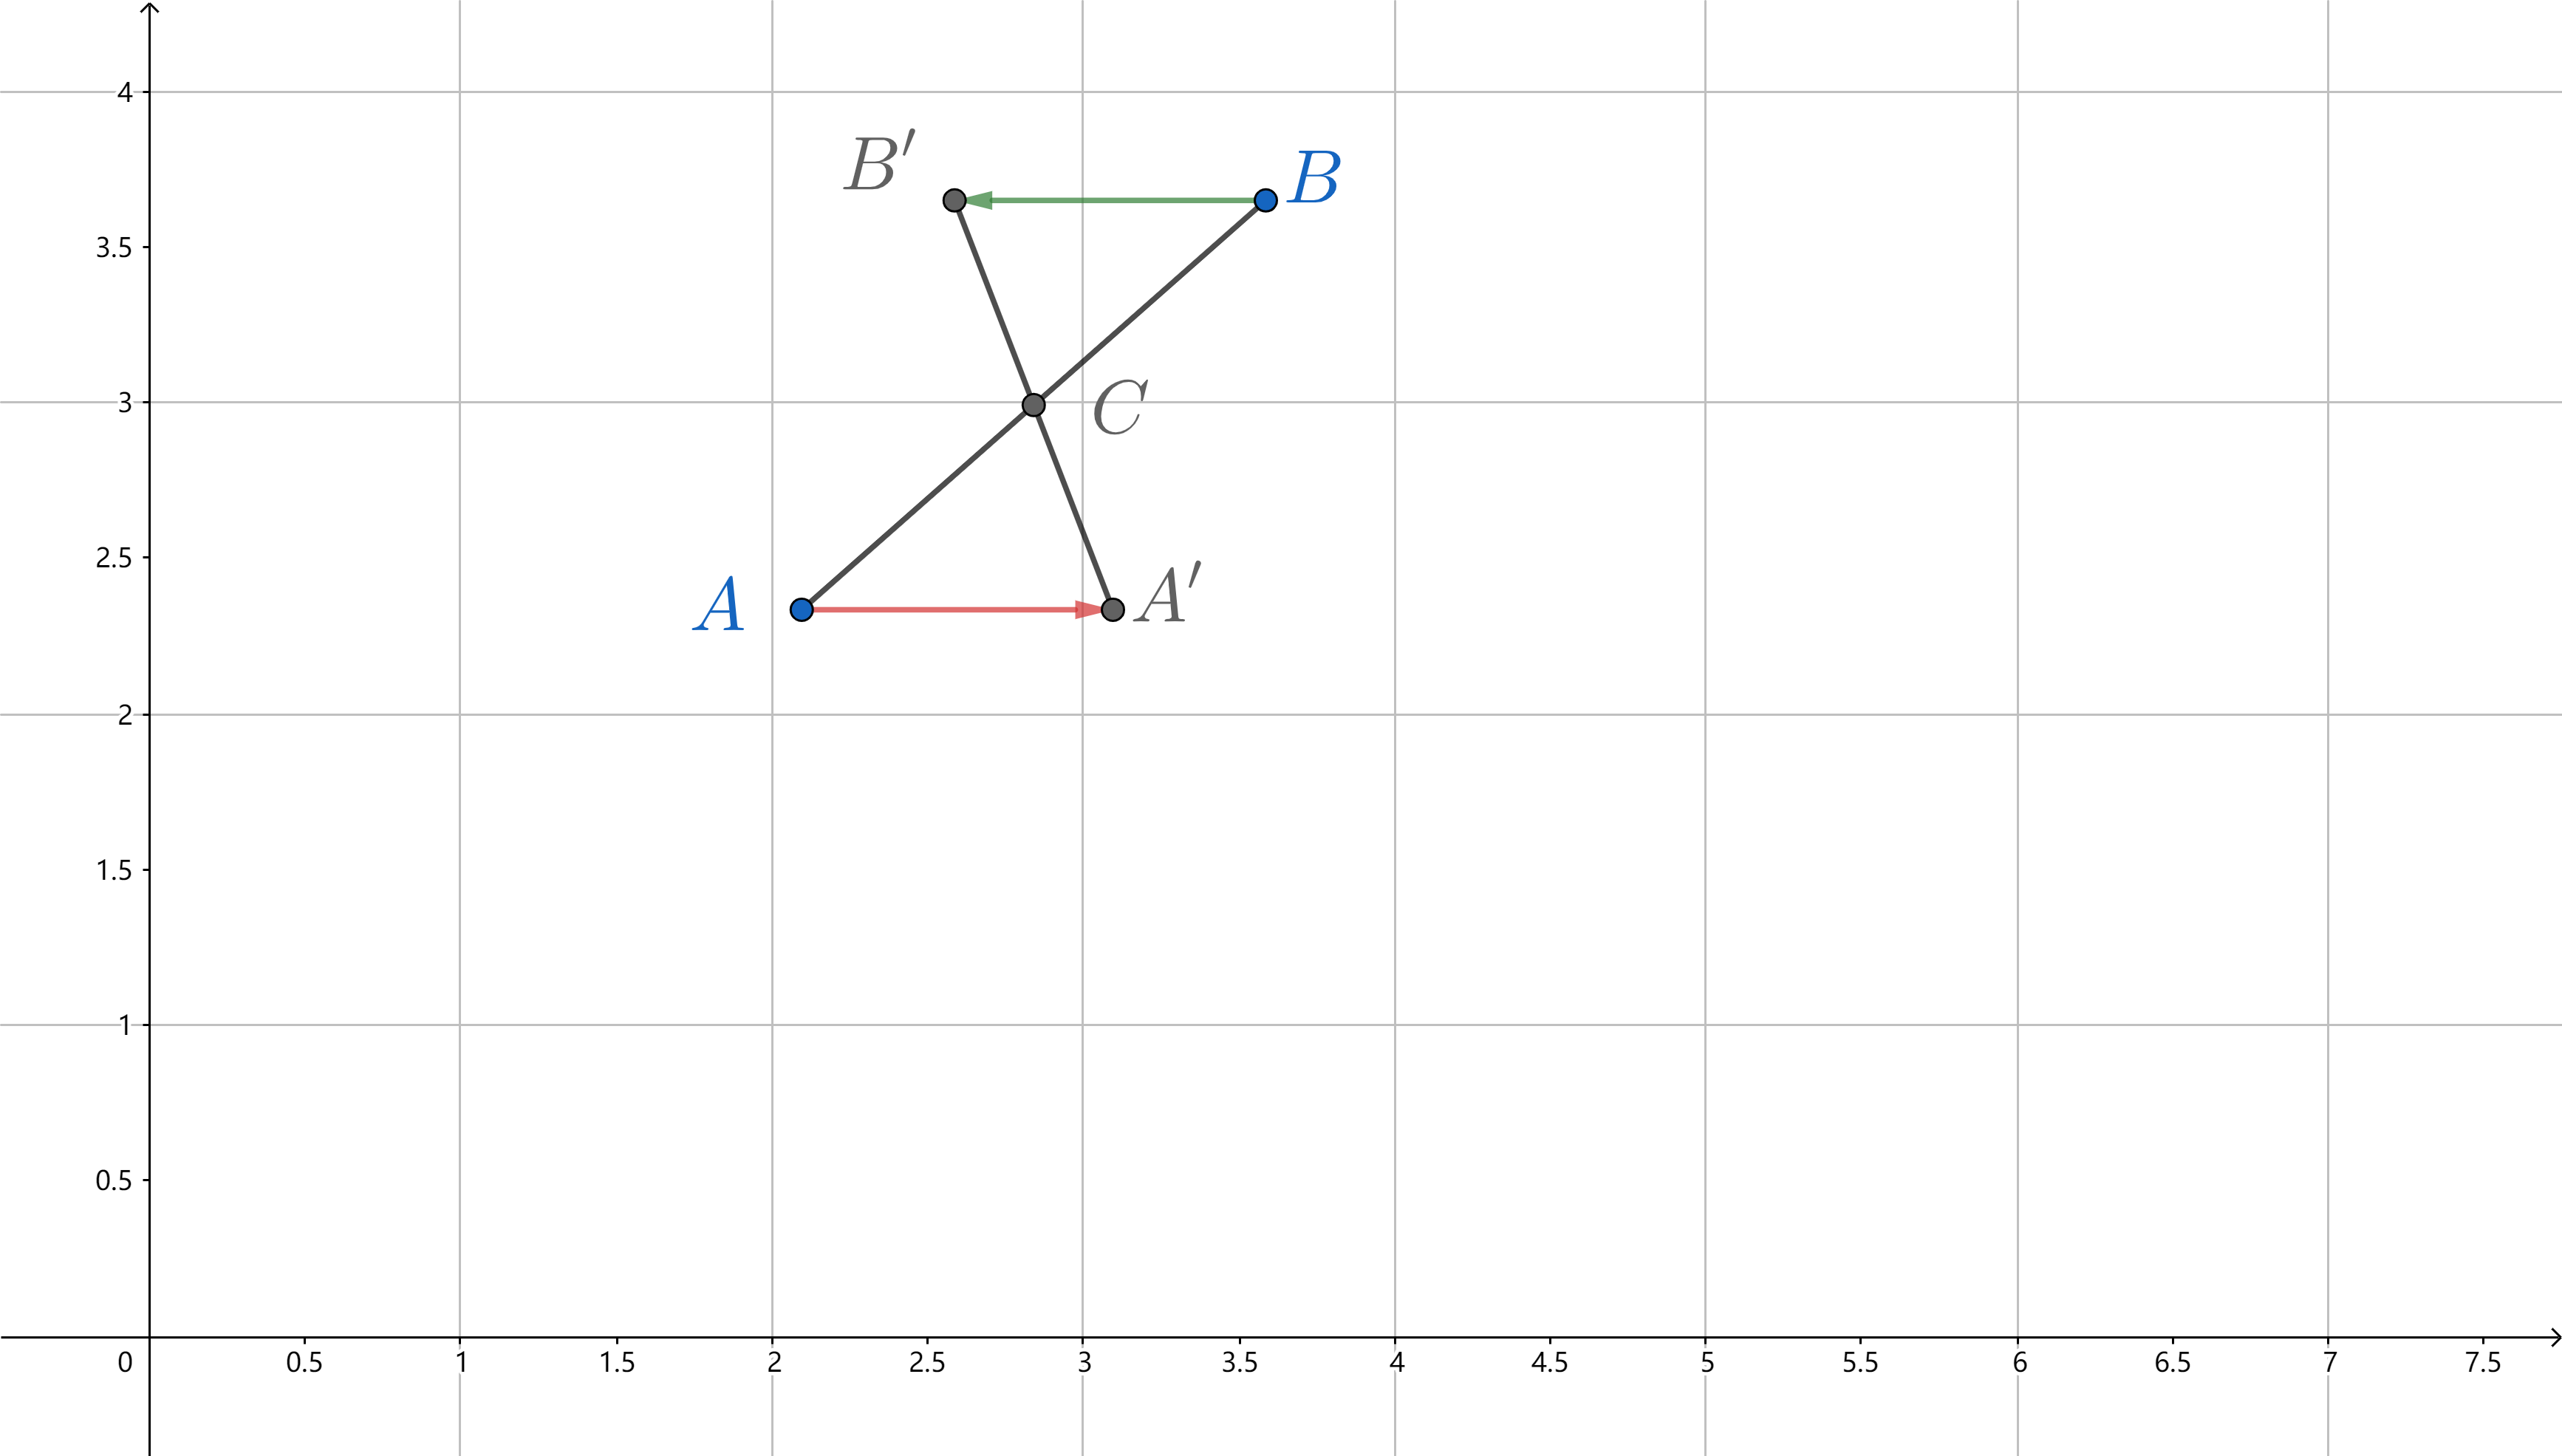
\includegraphics[width=5.76806in,height=3.27847in]{media/image6.png}

应用平移定理将 \(A\) 向右平移一个单位得到 \(A^{'}\),\(B\)
向左平移一个单位得到 \(B^{'}\),连 \(A^{'}B^{'}\) 交 \(AB\) 于
\(C\)。\(C\) 即为 \(AB\)
中点。由全等或者相似的知识可以很简单地证明此定理。我们可以用类似的方法得到三等分点、四等分点等,只需改变平移的单位长度即可。

\textbf{【证明】}\(\bigtriangleup BCB^{'} \sim \bigtriangleup ACA^{'}\),\(\frac{AC}{BC} = \frac{AA^{'}}{BB^{'}}\)。前面的证明可以同时证明定理本身和定理的扩展。

\hypertarget{ux63a8ux8bbaux500dux957fux7ebfux6bb5ux5b9aux7406-segment-multiplication-theoremux5b9aux7406-3.1.3}{%
\subsection{推论:倍长线段定理 Segment Multiplication Theorem(定理
3.1.3)}\label{ux63a8ux8bbaux500dux957fux7ebfux6bb5ux5b9aux7406-segment-multiplication-theoremux5b9aux7406-3.1.3}}

可以倍长任意线段。做法如下(倍长线段 \(AB\)):

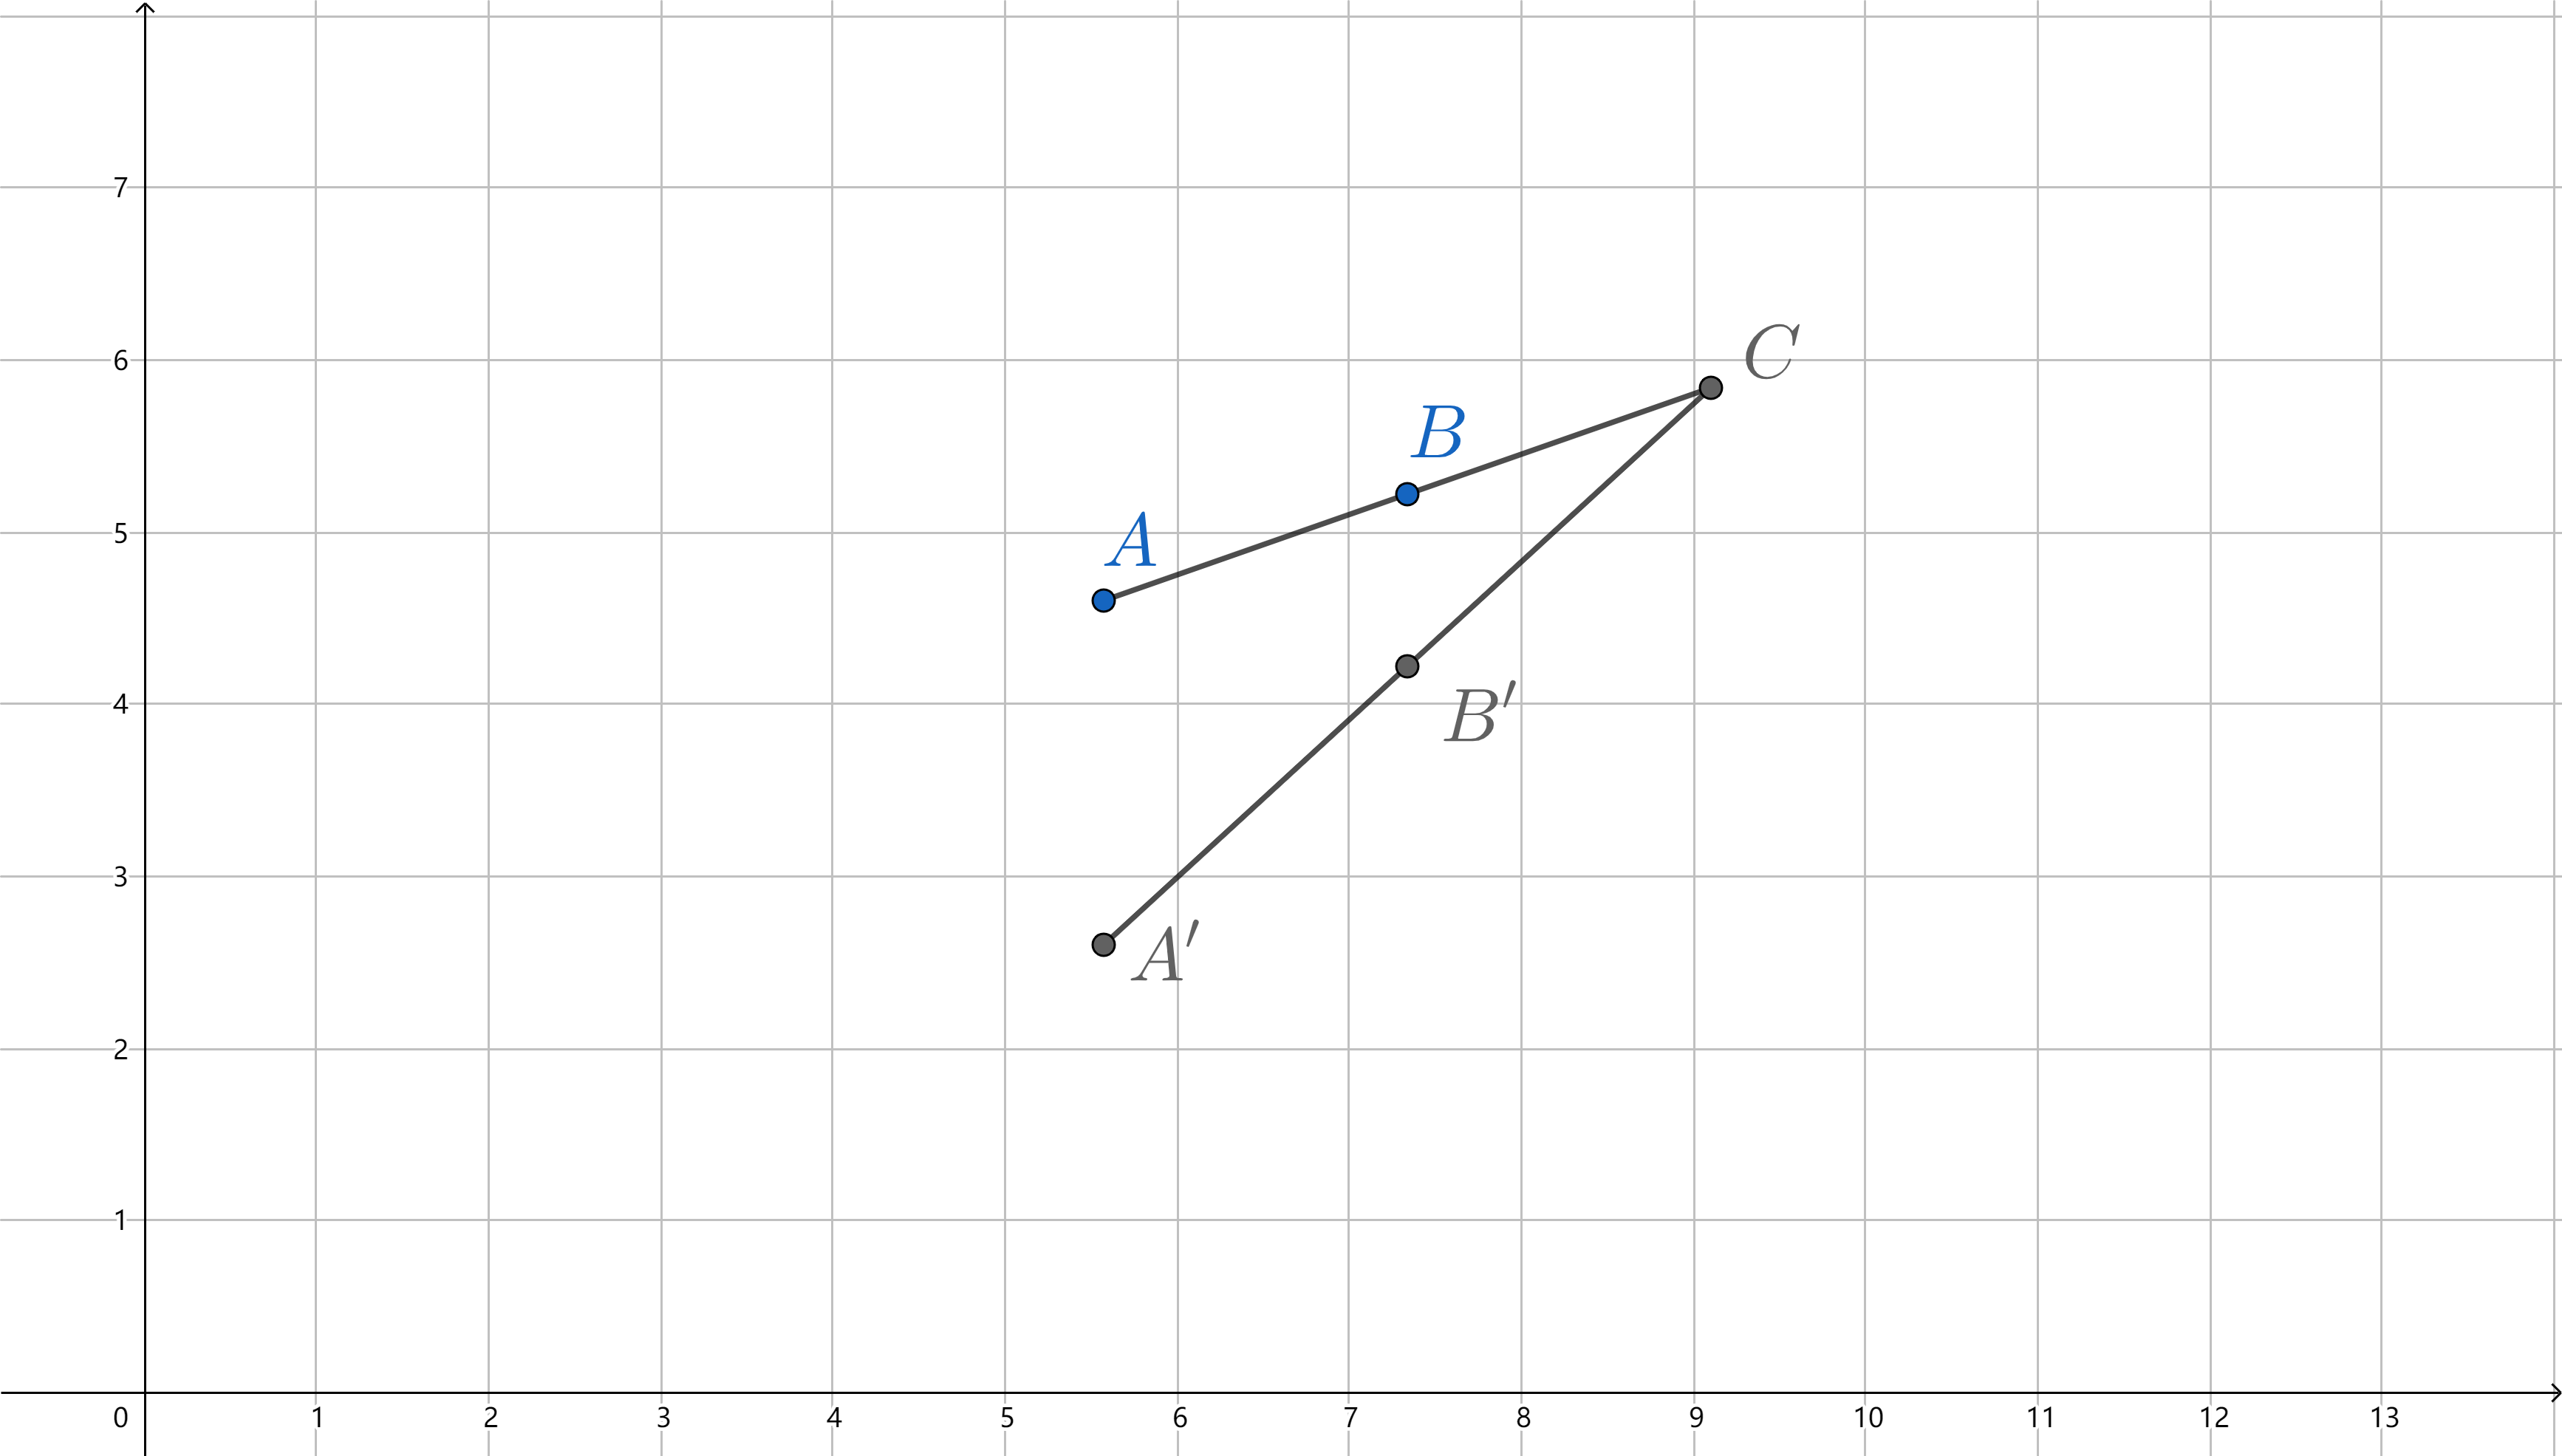
\includegraphics[width=5.76806in,height=3.27847in]{media/image7.png}

应用平移定理将 \(A\) 向下平移两个单位得到 \(A^{'}\),\(B\)
向下平移一个单位得到 \(B^{'}\),连 \(A^{'}B^{'}\) 并延长交 \(AB\) 于
\(C\)。此时
\(AB = BC = \frac{1}{2}AC\)。由相似的知识可以非常简单地证明此定理。

\textbf{【拓展】}通过改变向下平移的单位长度,可以做到三倍、四倍甚至3/2倍的倍长。

\textbf{【证明】}\(\bigtriangleup CBB^{'} \sim \bigtriangleup CAA^{'}\),\(\frac{AC}{BC} = \frac{AA^{'}}{BB^{'}}\)。前面的证明可以同时证明定理本身和定理的拓展。

郝铭扬在 2022年 6 月 12 日
给出了Zyk基本对称定理的优化,这也被称为``绵羊把戏(Sheep's trick)''。

\hypertarget{zykux57faux672cux5bf9ux79f0ux5b9aux7406ux7684hmyux7b2cux4e00ux4f18ux5316-hmys-first-optimization-of-zyks-basic-symmetry-theoremux5b9aux7406-3.1.4}{%
\subsection{Zyk基本对称定理的Hmy第一优化 Hmy's First Optimization of
Zyk's Basic Symmetry Theorem(定理
3.1.4)}\label{zykux57faux672cux5bf9ux79f0ux5b9aux7406ux7684hmyux7b2cux4e00ux4f18ux5316-hmys-first-optimization-of-zyks-basic-symmetry-theoremux5b9aux7406-3.1.4}}

\textbf{【提出者】}郝铭扬

可以用稍微简单一点的方法作任意点关于一条格线的对称,作图方法如下:

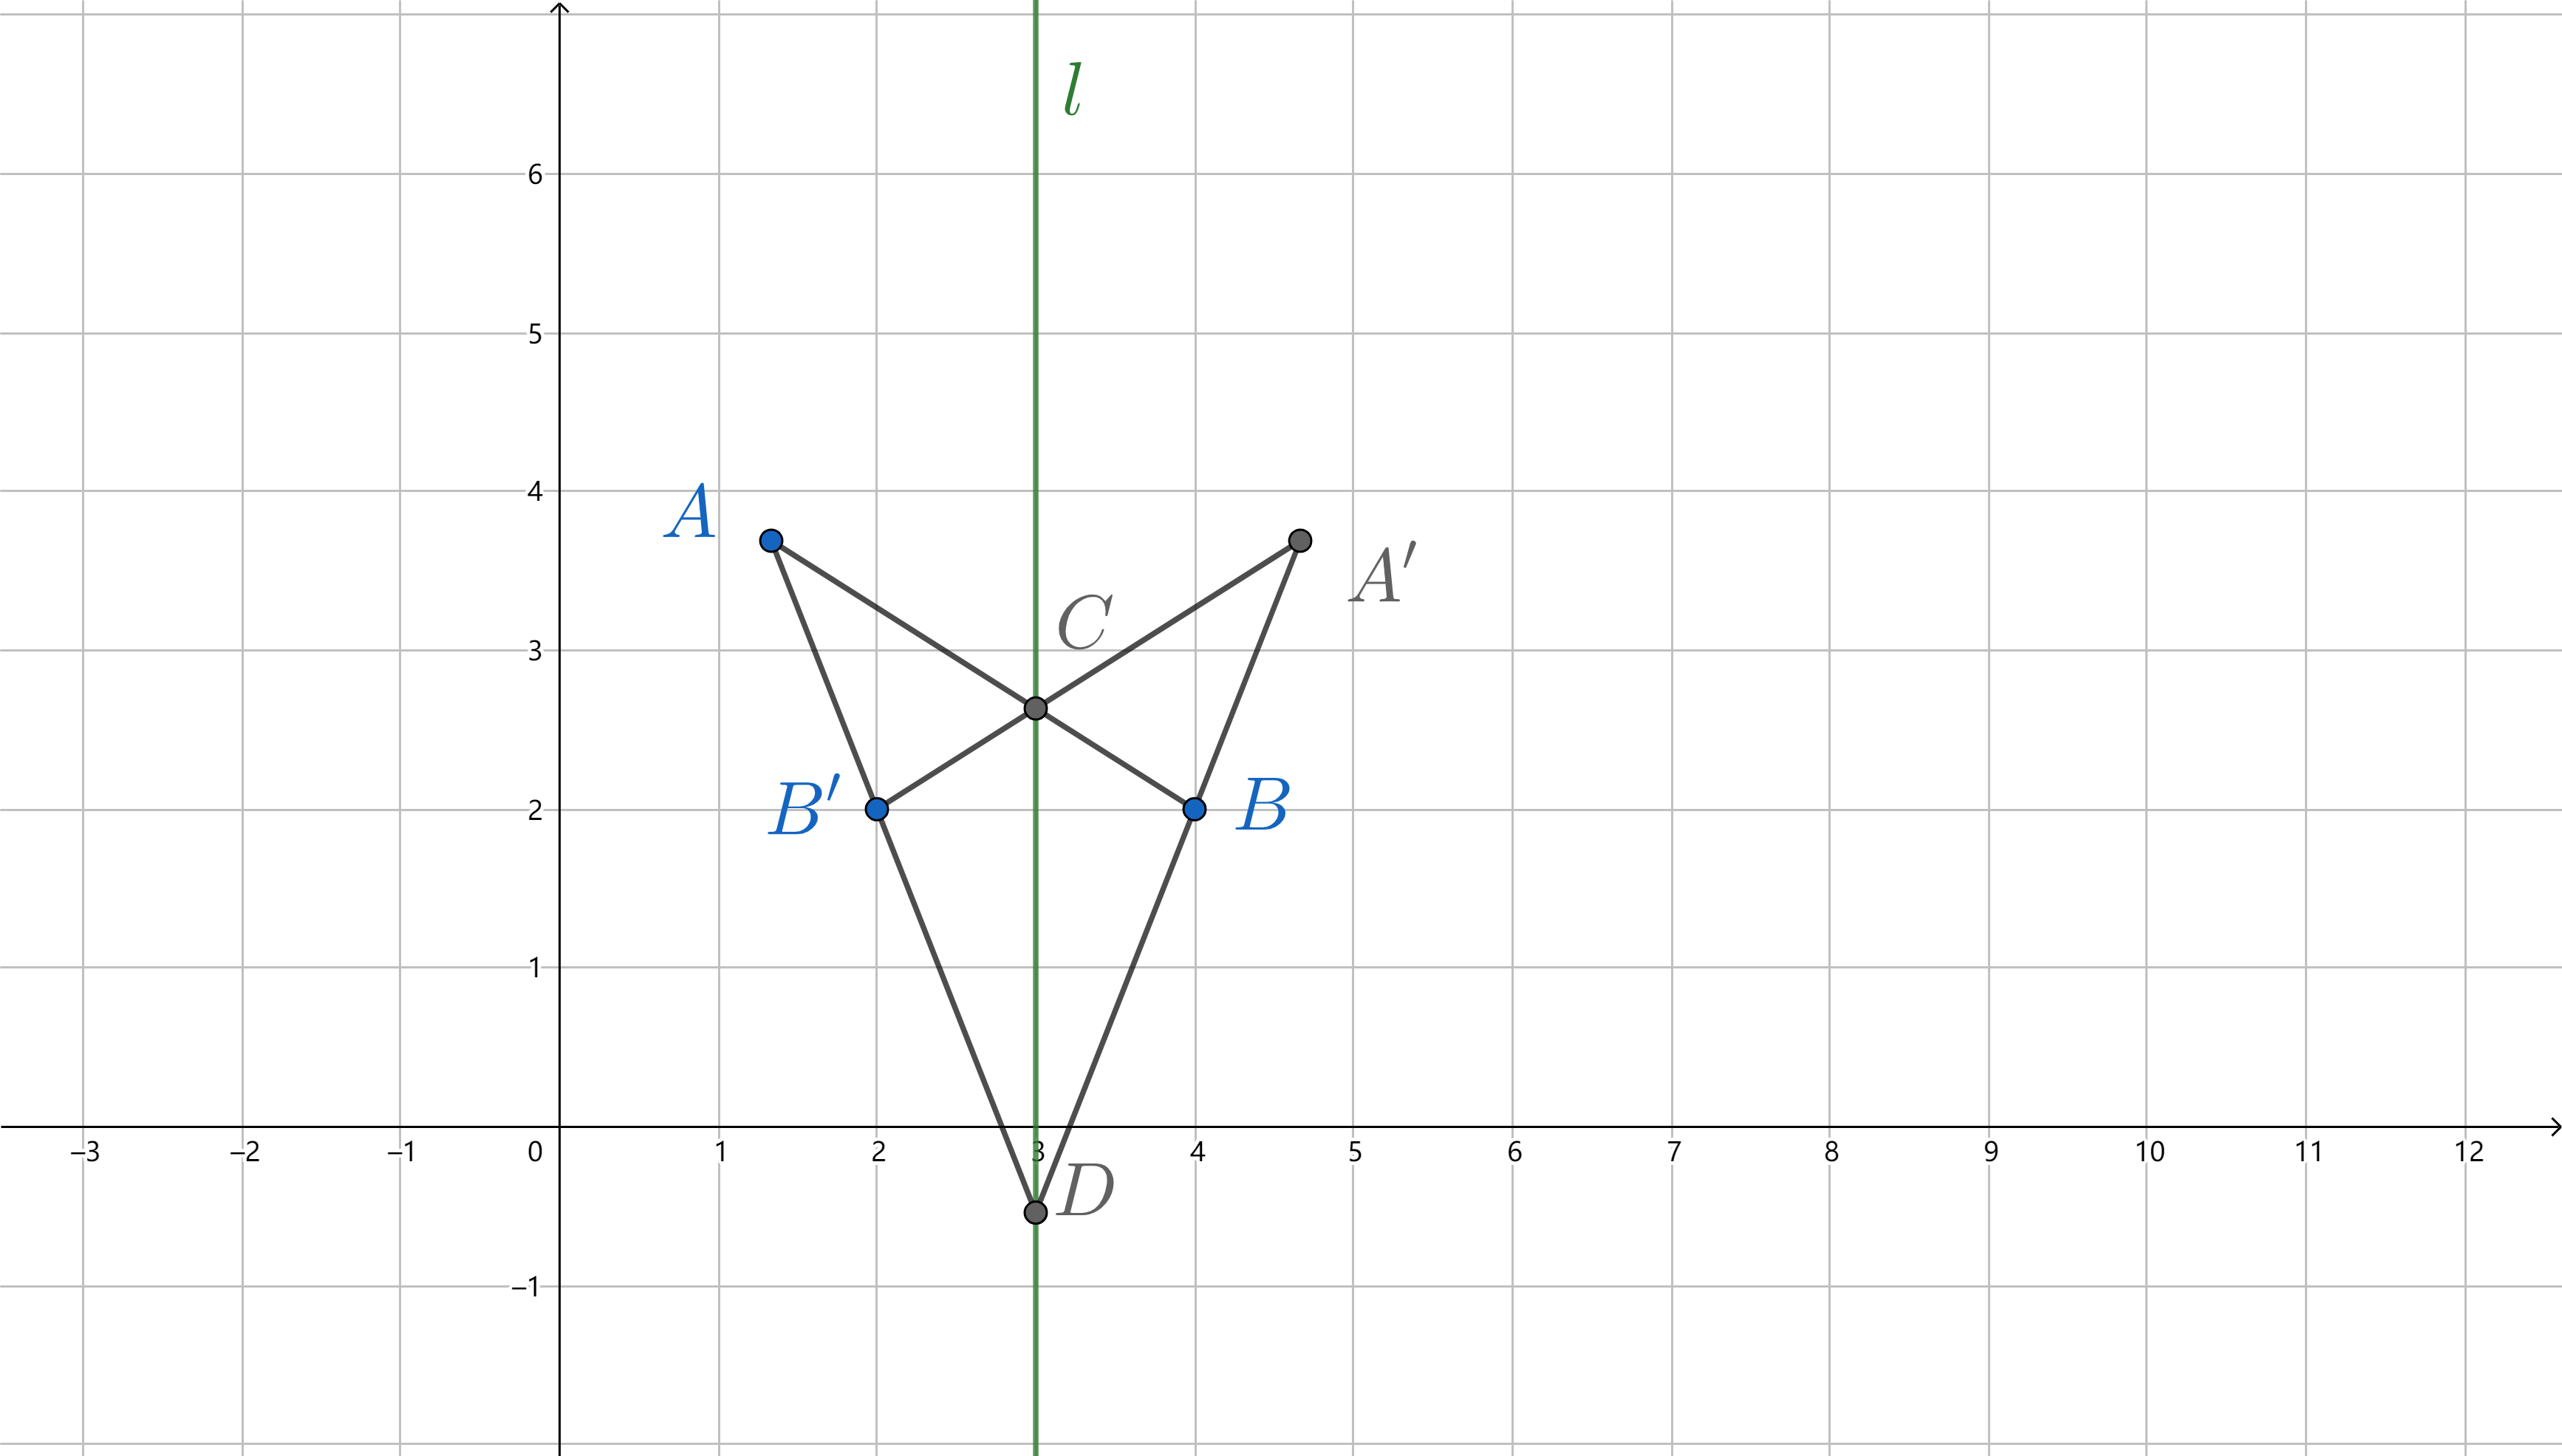
\includegraphics[width=5.76806in,height=3.27847in]{media/image8.png}

\textbf{【作图语句】}选定格点 \(B\),\(B^{'}\)(要求 \(B\),\(B^{'}\)
关于 \(l\) 对称),连接 \(AB\),\(AB^{'}\) 并延长分别交 \(l\) 于
\(C\),\(D\)。连接 \(B^{'}C\),\(DB\) 并延长交于 \(A^{'}\)。\(A^{'}\)
即为所求。

\textbf{【证明】}不难发现直线 \(AB\) 和直线 \(A^{'}B^{'}\) 对称,直线
\(AD\) 与直线 \(A^{'}D^{'}\) 对称,所以直线的交点也对称,这样 \(A\) 和
\(A^{'}\) 就是对称的了。

\hypertarget{zsqux5e73ux884cux5b9aux7406}{%
\subsubsection{Zsq平行定理}\label{zsqux5e73ux884cux5b9aux7406}}

Zsq同学解决了过任意点做任意直线平行线的问题。其实,只用Zyk基本对称定理及其推论也可以实现,但是Zsq平行定理更加简洁。我们先讲如何只用Zyk基本对称定理及其推论来实现。

如图,\(A\) 为任意点,\(l\) 为任意直线,过 \(A\) 做
\(l_{2} \parallel l\)。

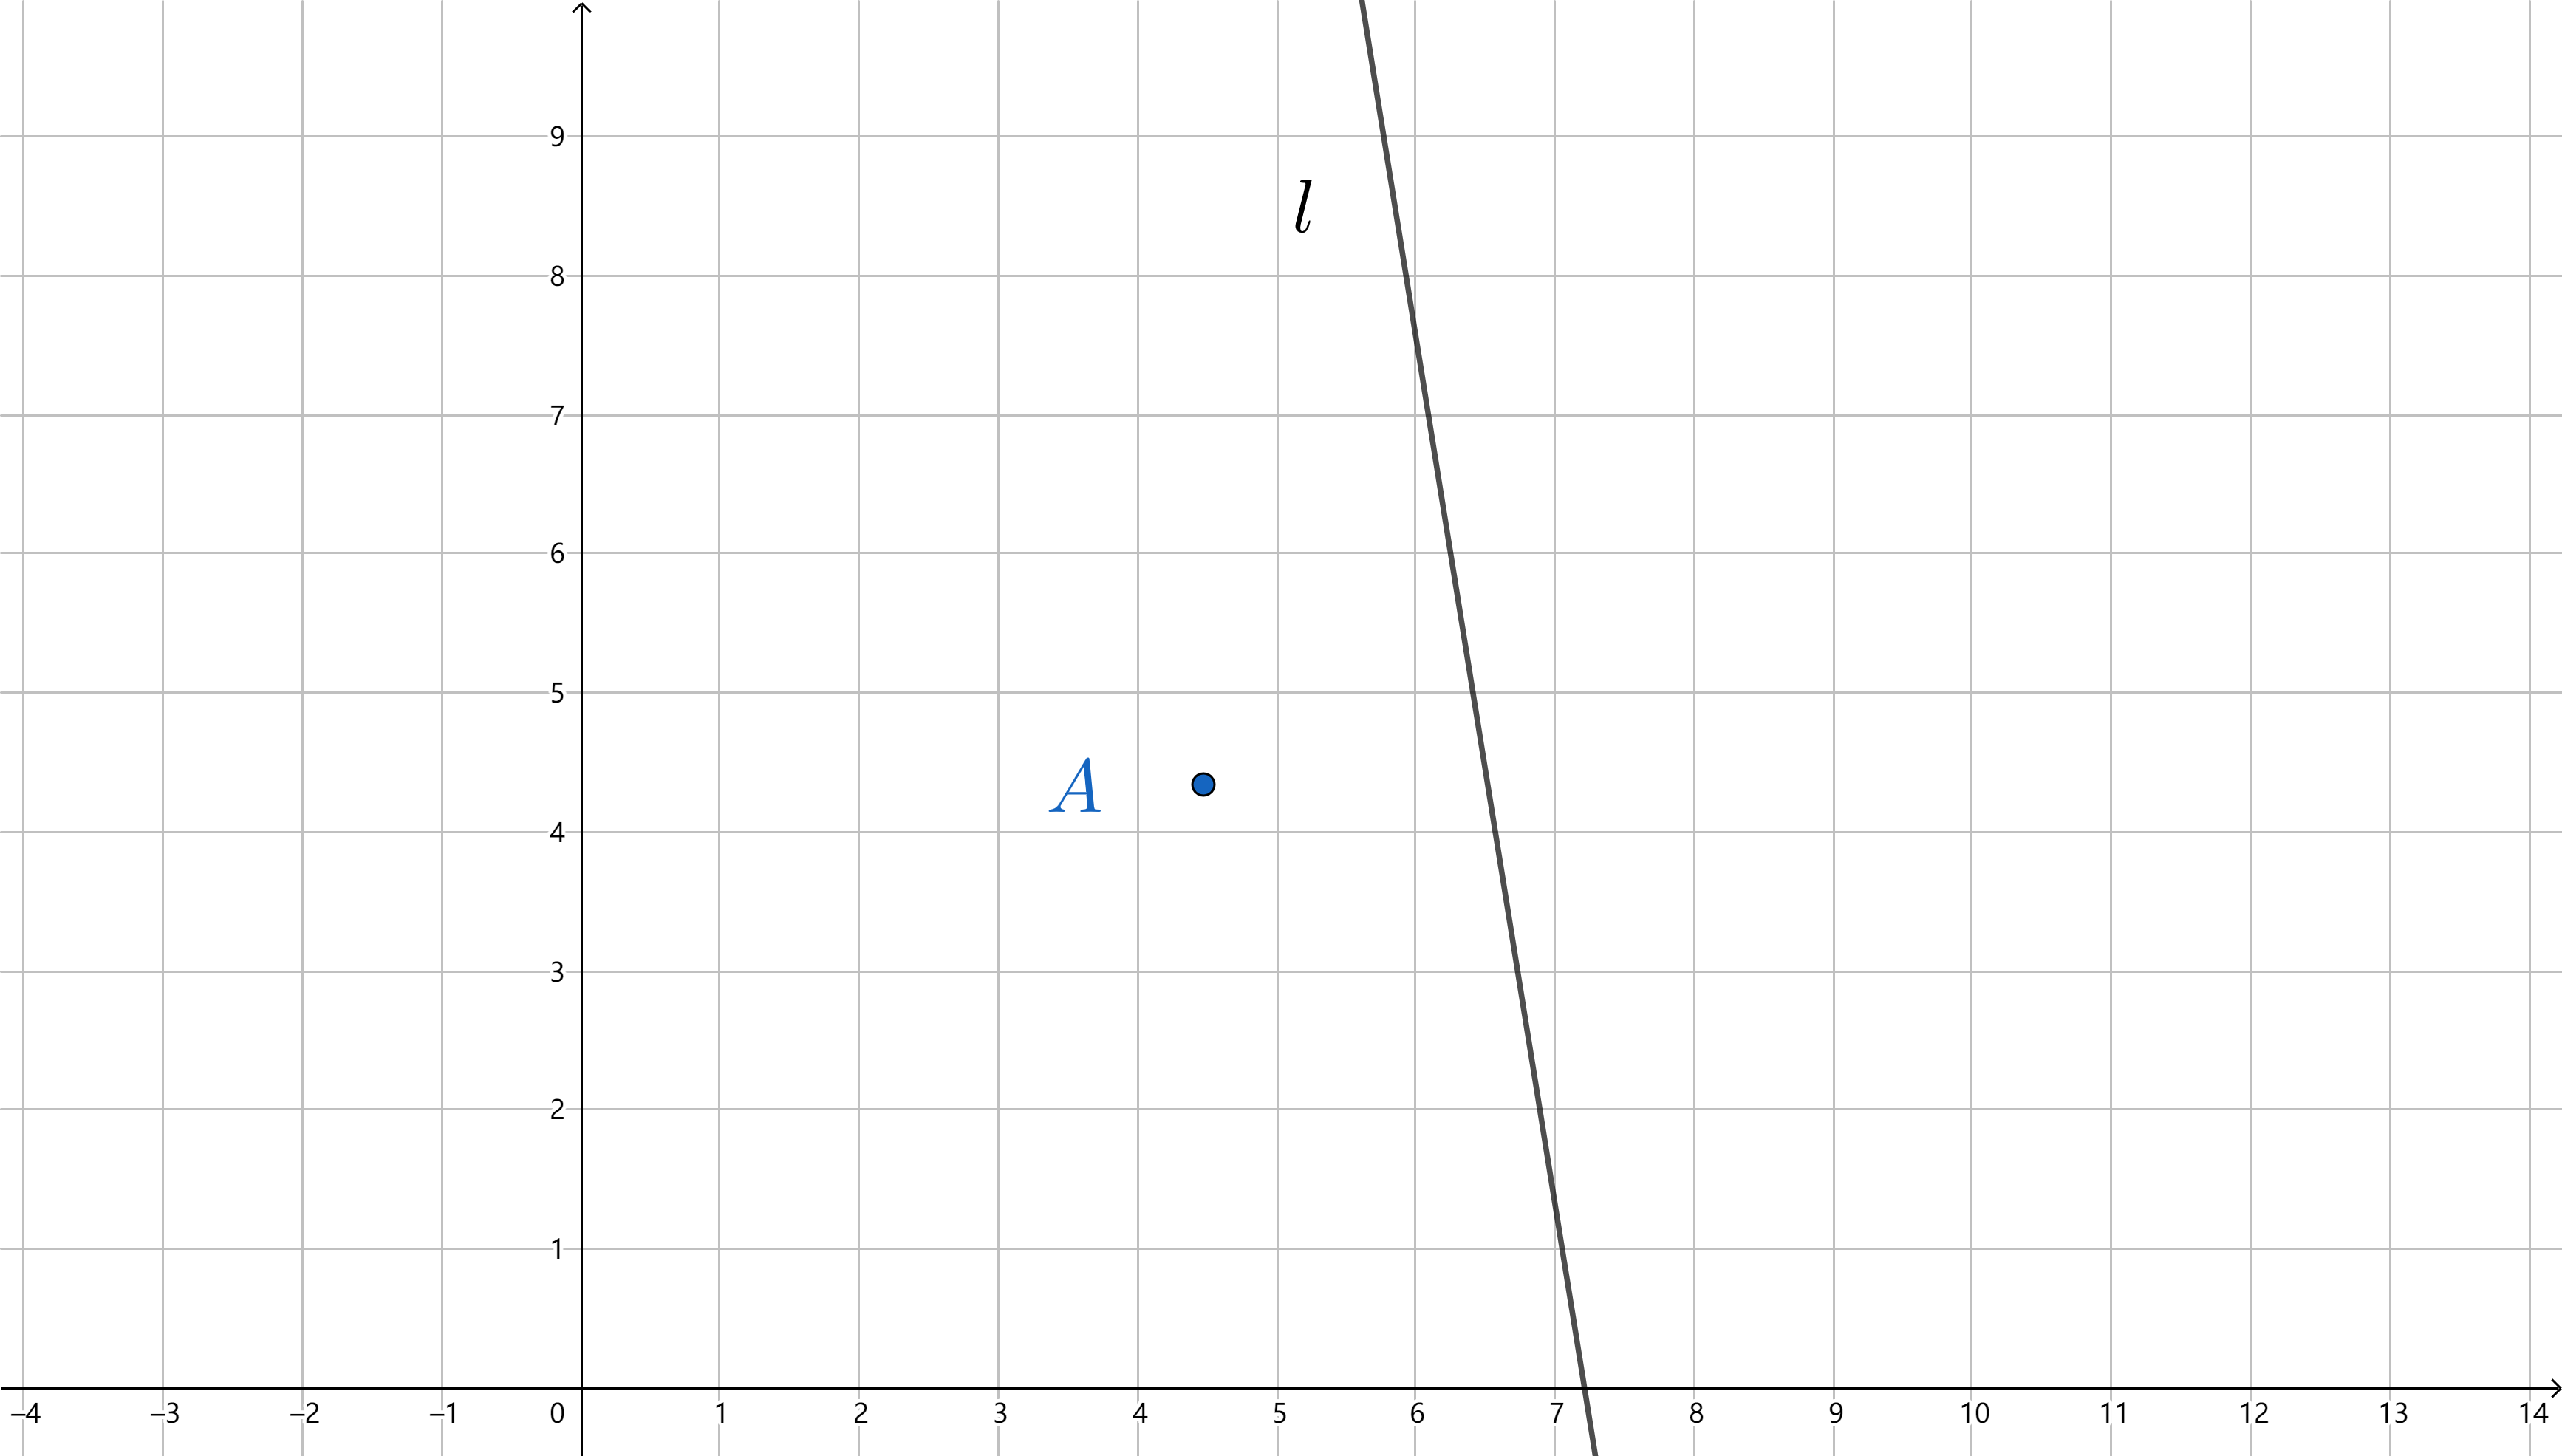
\includegraphics[width=5.76806in,height=3.27847in]{media/image9.png}

我们可以通过构造中位线的方法来解决这个问题。

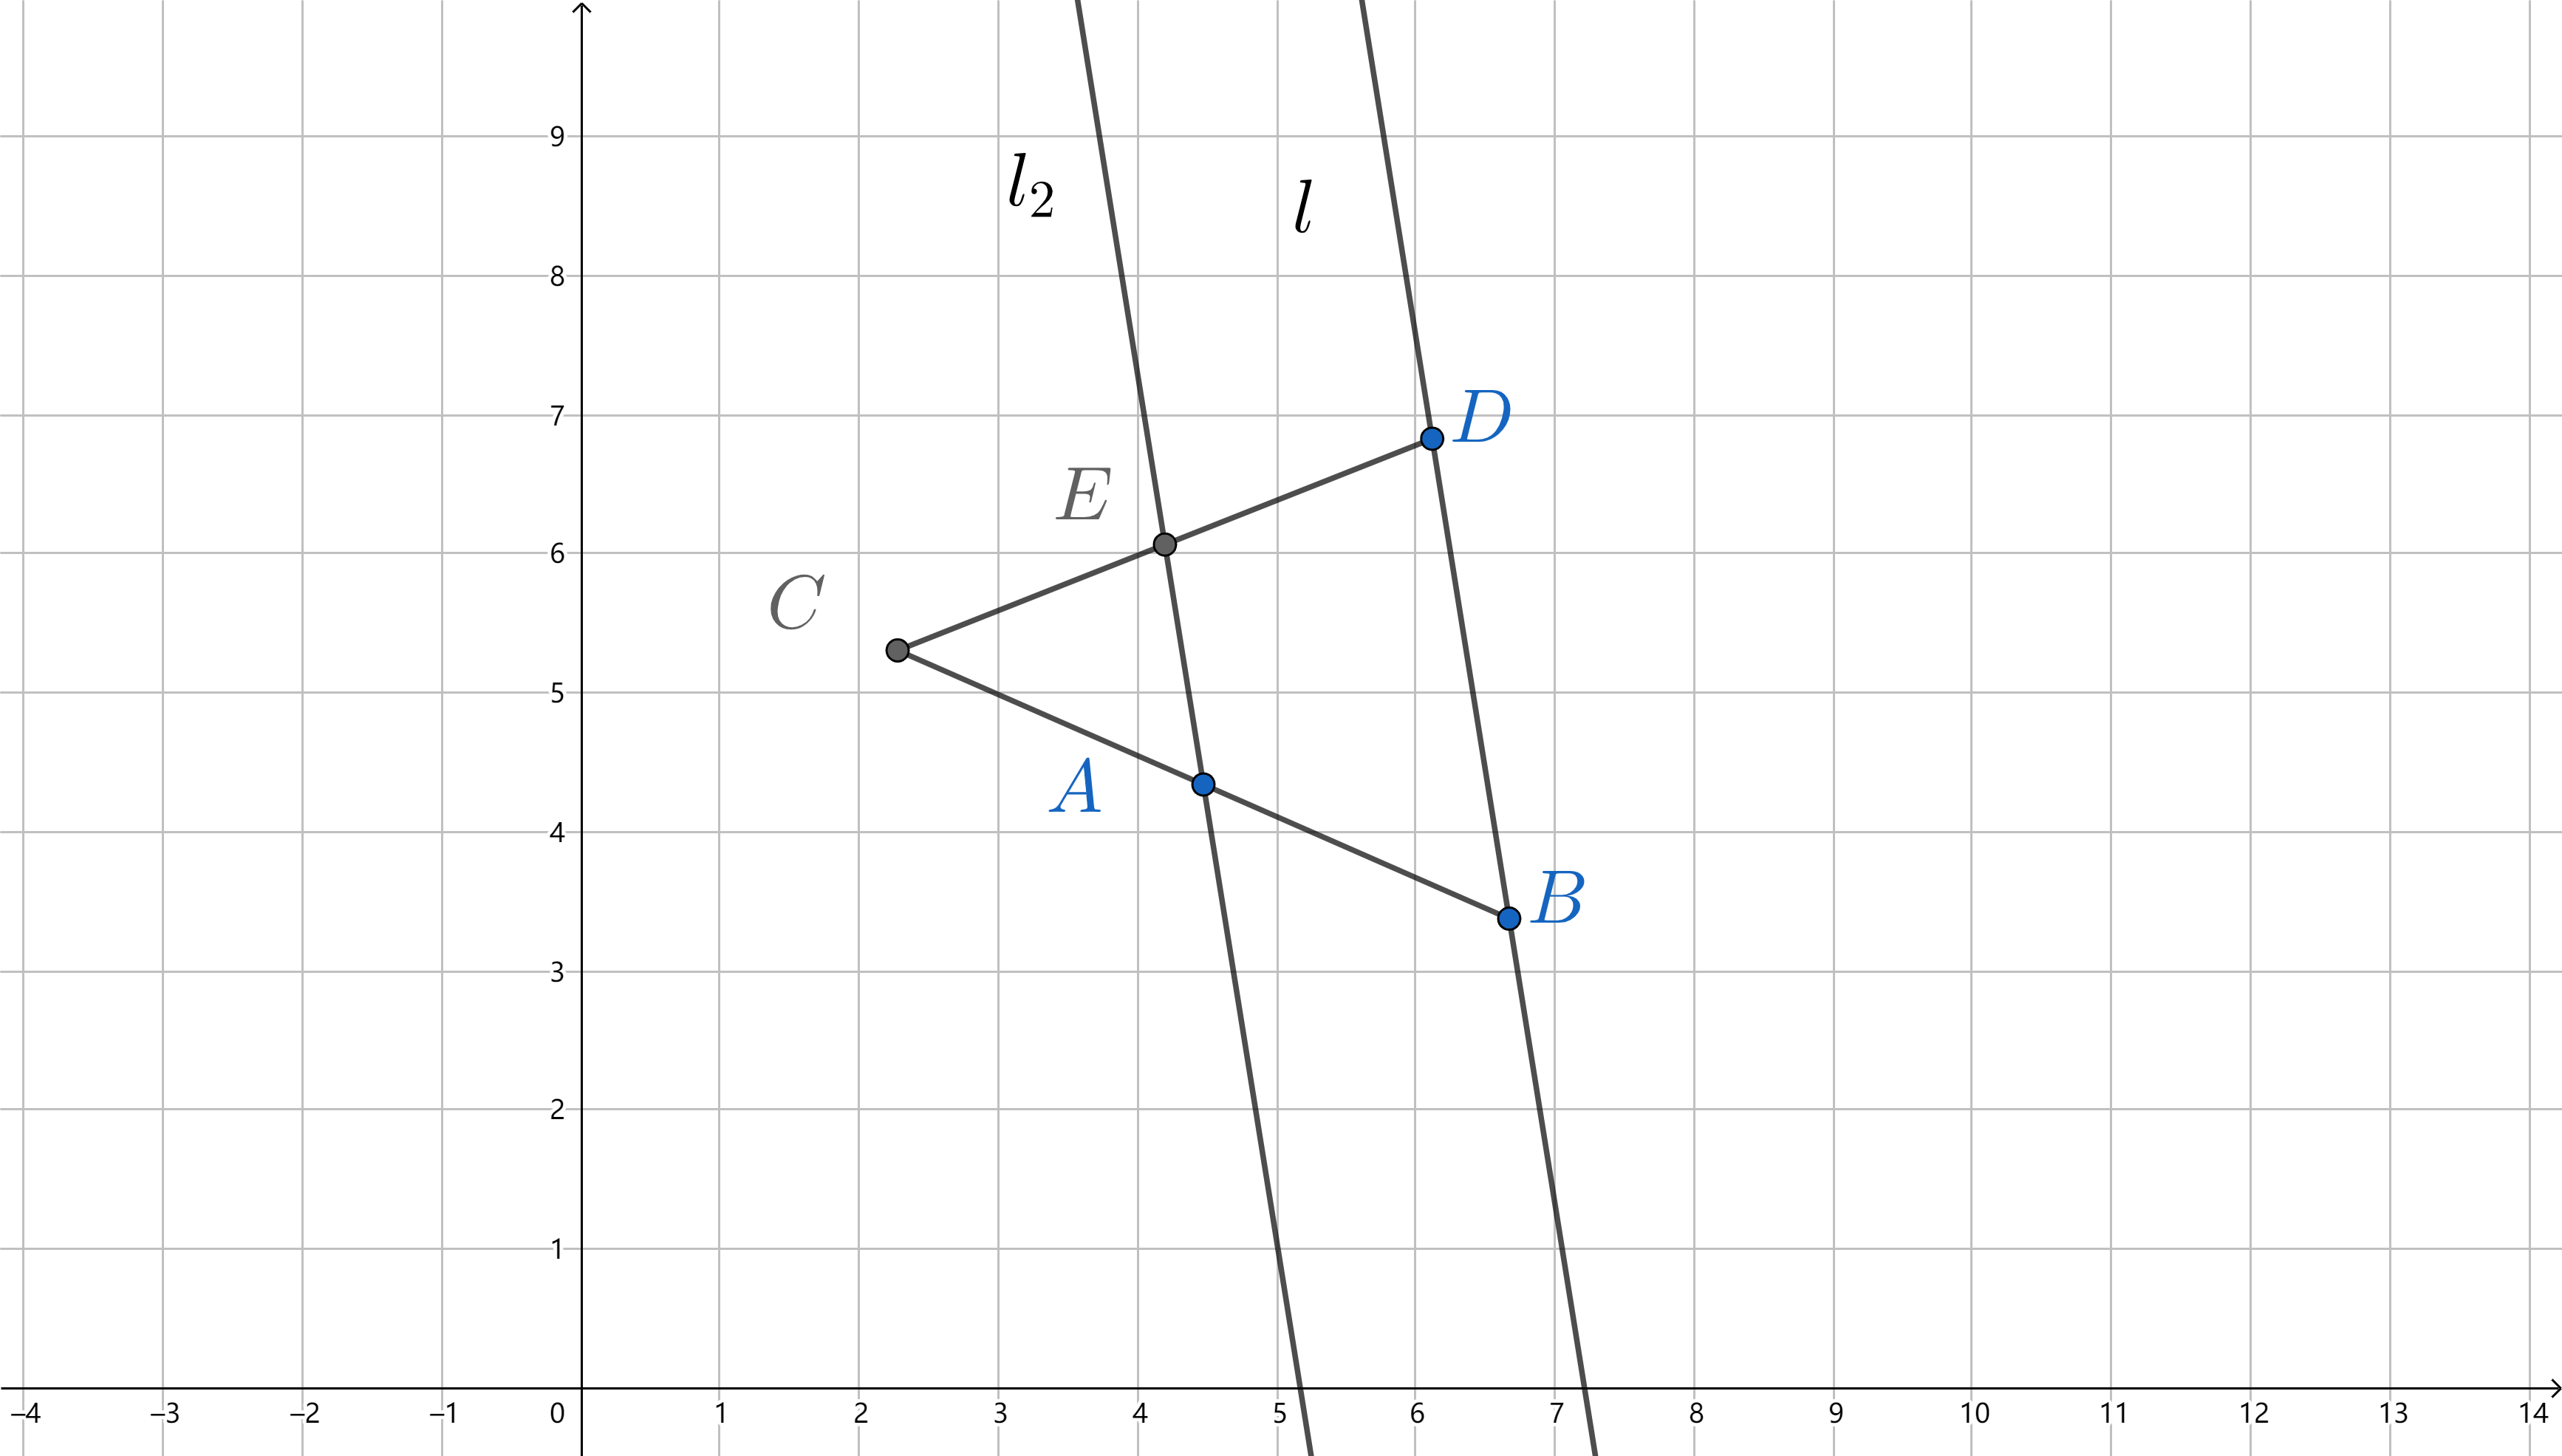
\includegraphics[width=5.76806in,height=3.27847in]{media/image10.png}

首先,在直线 \(l\) 上取合适的一点 \(B\),应用倍长线段定理(定理
3.1.3)倍长线段 \(BA\) 到 \(C\)。再在直线上取合适的一点 \(D\),连接
\(CD\),应用平分线段定理(定理 3.1.2)得到 \(CD\) 的中点 \(E\)。连接
\(AE\),\(AE\) 即为所求。

这种方法非常容易理解,但是作图非常繁琐。Zsq平行定理巧妙地运用塞瓦定理,使得其作图方法非常简单,我们来看一下作图方法。

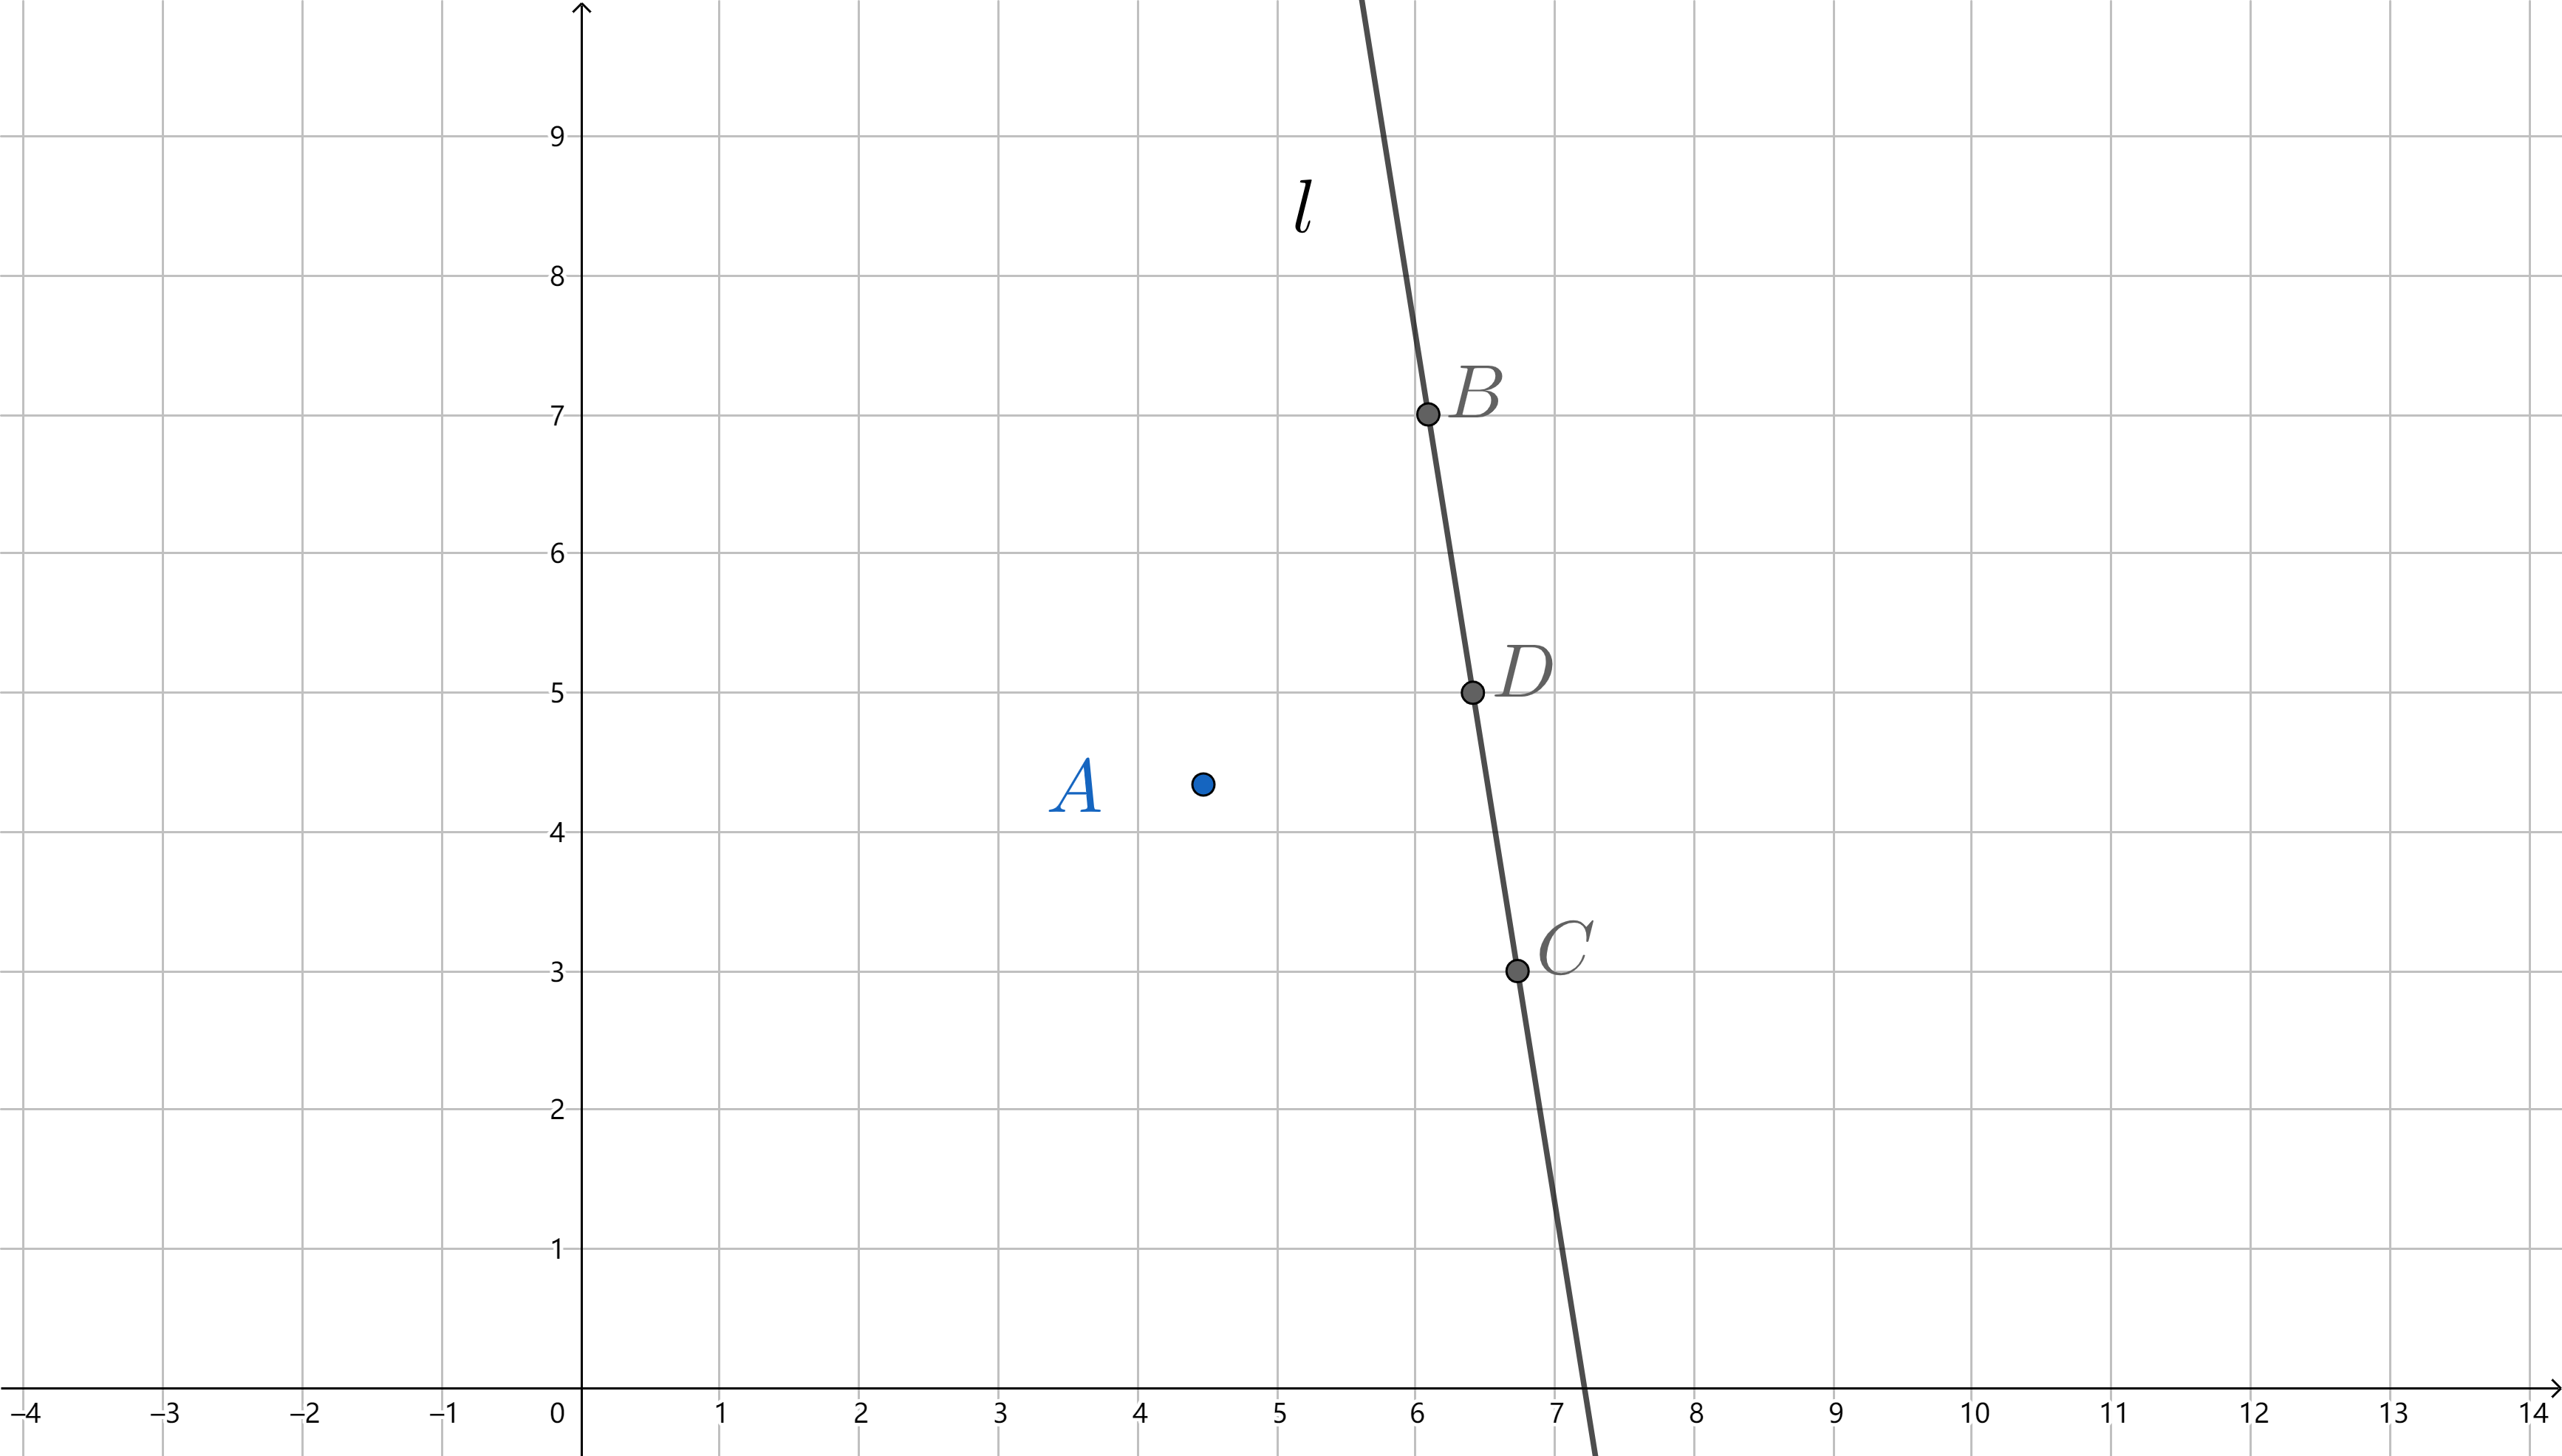
\includegraphics[width=5.76806in,height=3.27847in]{media/image11.png}

首先我们要选取三个点
\(B\),\(D\),\(C\)。这三个点不是随便选取的,它们都是直线 \(l\)
与水平格线的交点,而且 \(B\) 和 \(D\)、\(D\) 和 \(C\)
的垂直距离是相等的,这也就意味着 \(D\) 是线段 \(BC\)
的中点。选择竖直格线上等距离三点也是可以的,无论怎样选择根本目的都是让
\(D\) 为 \(BC\) 中点。此时我们连接 \(CA\) 并延长并在延长线上取一点 \(E\)
并连接 \(BE\)。

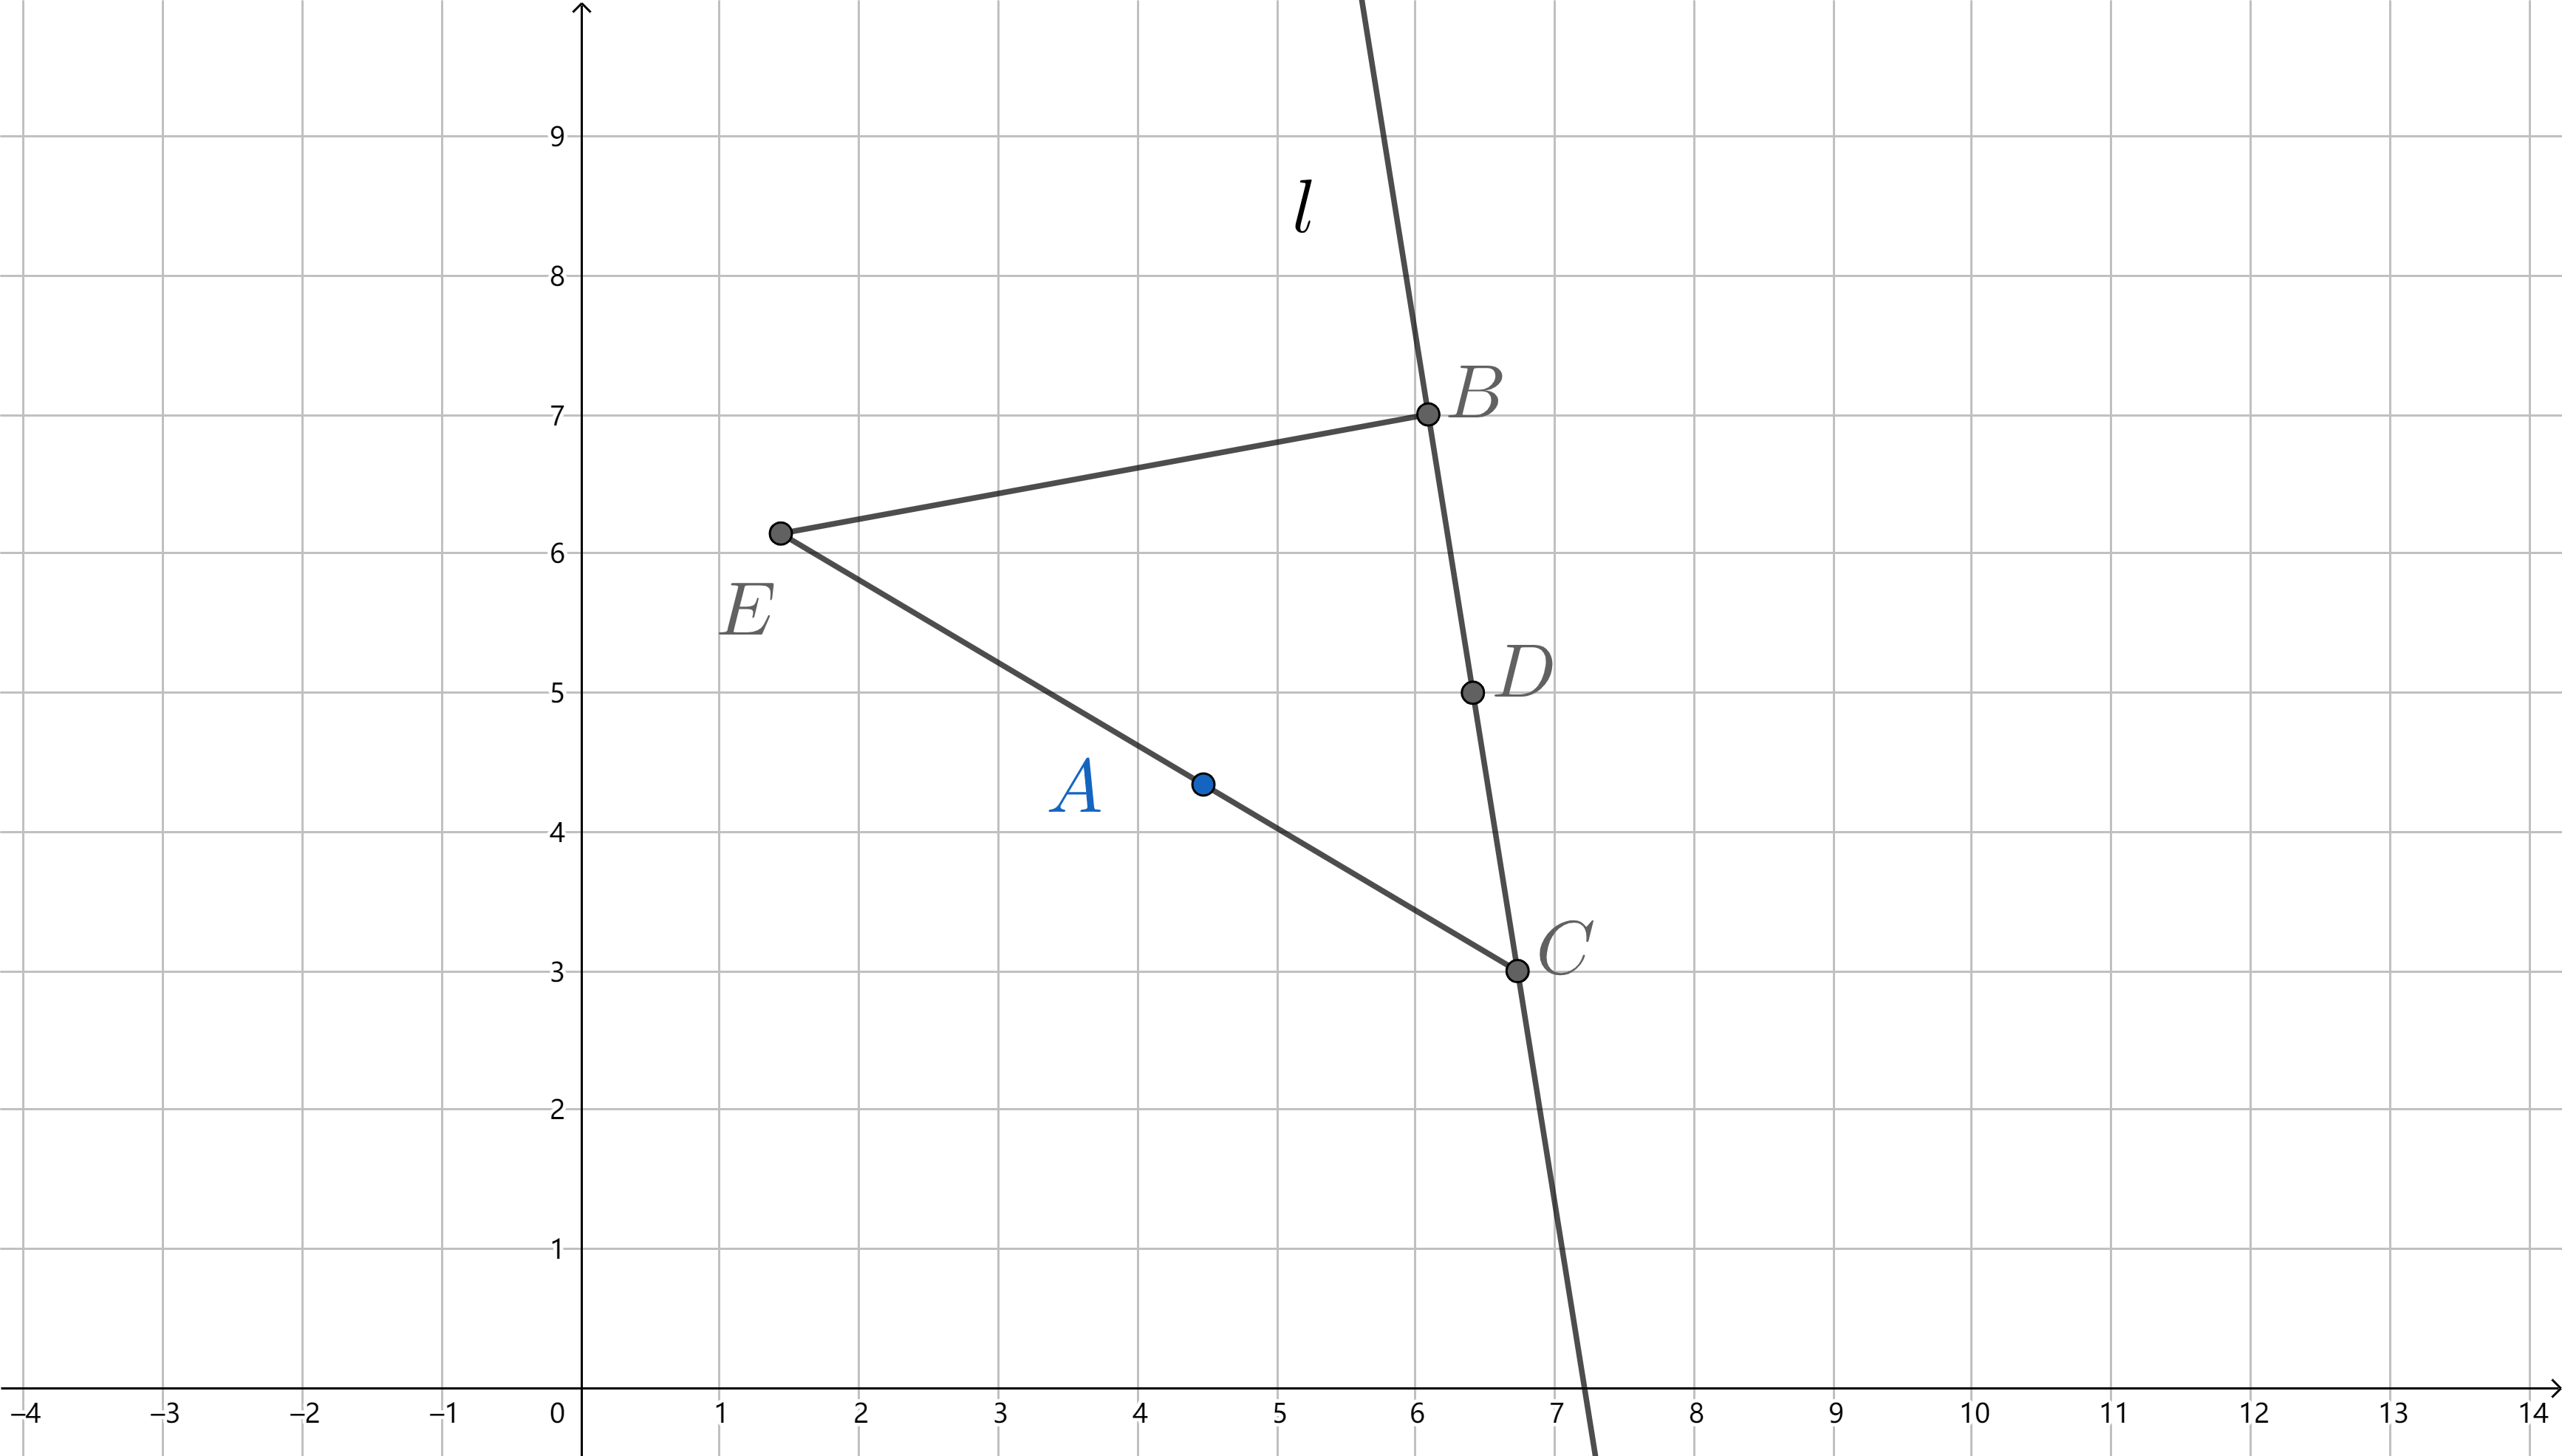
\includegraphics[width=5.76806in,height=3.27847in]{media/image12.png}

此时我们连接 \(ED\),\(BA\) 交于 \(F\)。连接 \(CF\) 并延长交 \(EB\) 于
\(G\)。连 \(AG\),\(AG\) 即为所求。

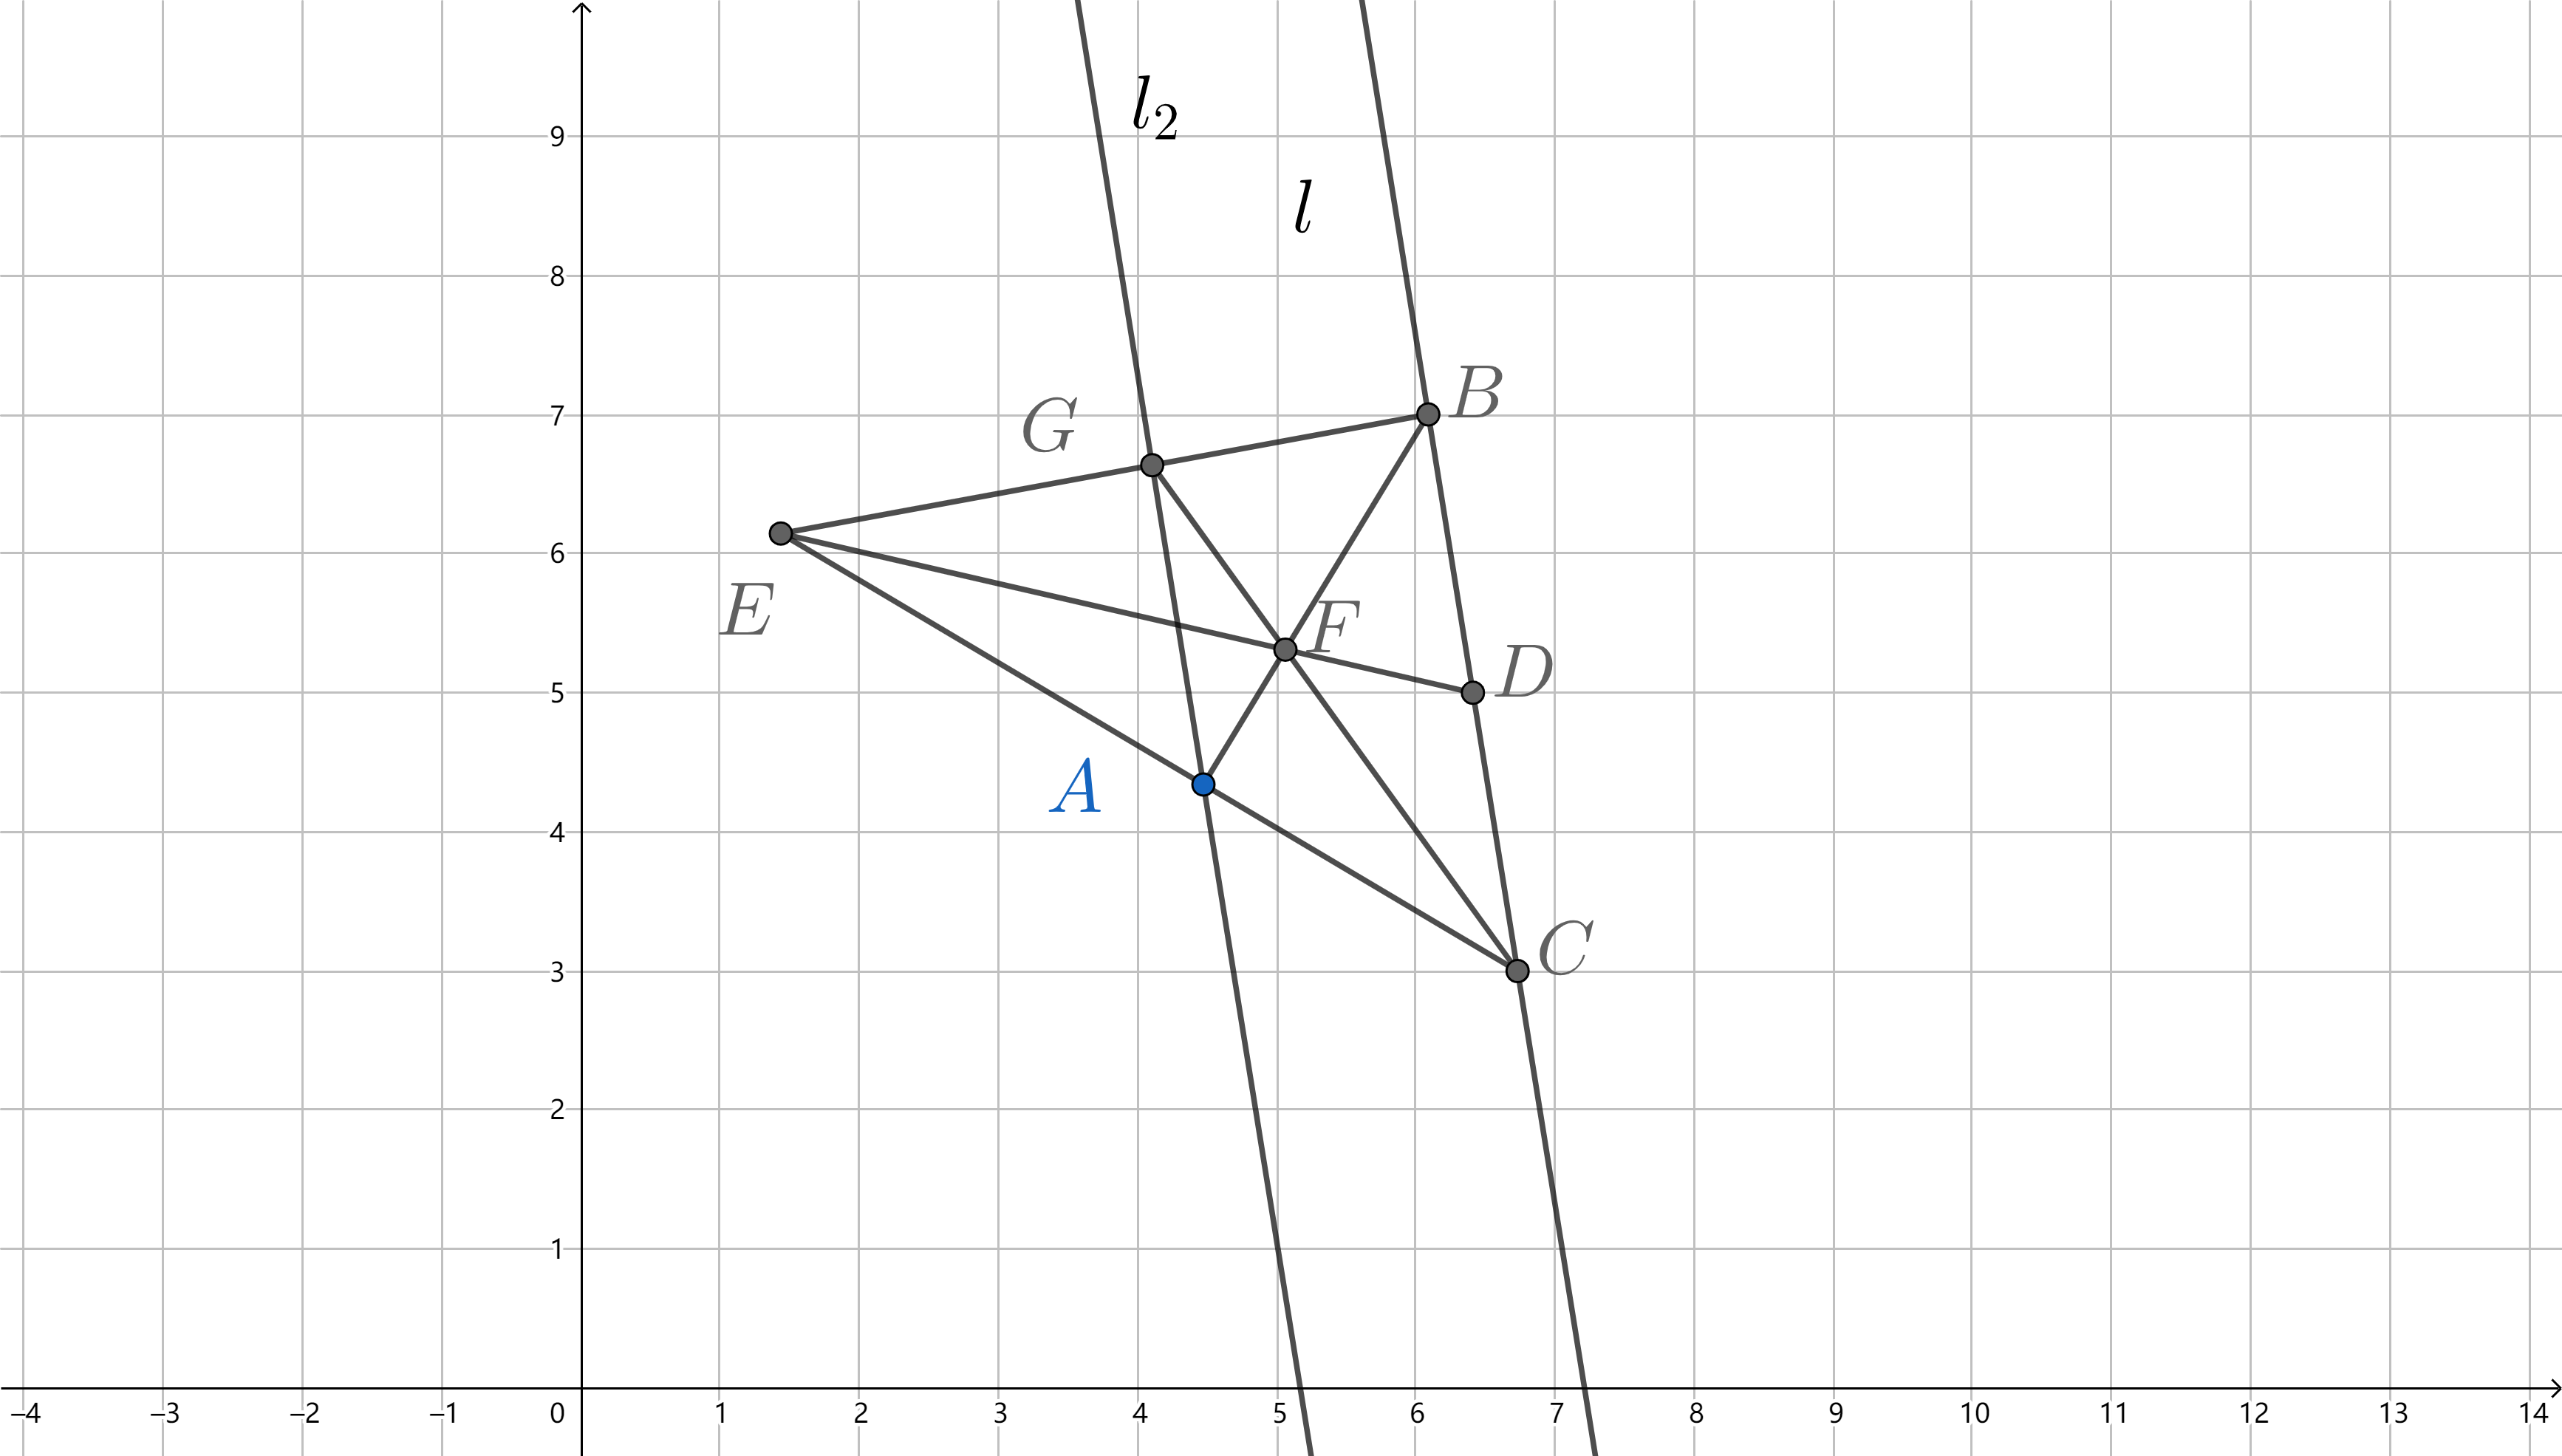
\includegraphics[width=5.76806in,height=3.27847in]{media/image13.png}

\textbf{【证明】}这个定理的证明并不显然,我们来尝试证明一下。这里出现了三角形内三线共点的情况,这让我们想到了塞瓦定理。

\[\frac{EA}{AC} \cdot \frac{CD}{DB} \cdot \frac{BG}{GE} = 1\]

因为 \(D\) 是 \(BC\) 的中点,所以
\(\frac{CD}{BD} = 1\),表达式被化简为:

\[\frac{EA}{AC} \cdot \frac{BG}{GE} = 1\]

再移项变换,可以得到

\[\frac{EA}{AC} = \frac{EG}{BG}\]

可以判定

\[\mathrm{\Delta}EAG \sim \mathrm{\Delta}ECB\]

所以 \(AG \parallel BC\)。结论得证

\hypertarget{zsqux5e73ux884cux5b9aux7406-zsqs-parallel-theoremux5b9aux7406-3.2}{%
\subsection{Zsq平行定理 Zsq's Parallel Theorem(定理
3.2)}\label{zsqux5e73ux884cux5b9aux7406-zsqs-parallel-theoremux5b9aux7406-3.2}}

\textbf{【提出者】}张世其

可以过任意一点做任意一条直线的平行线。

Zyk基本对称定理和Zsq平行定理的提出,让任意点网格作图不再是天方夜谭,为任意点作图奠定了基础。此后,越来越多的高级定理被发现。

\hypertarget{ux6734ux7d20ux5e73ux79fbux5b9aux7406}{%
\subsubsection{朴素平移定理}\label{ux6734ux7d20ux5e73ux79fbux5b9aux7406}}

这是一个比较简单的定理,我们直接介绍做法。

\hypertarget{ux6734ux7d20ux5e73ux79fbux5b9aux7406-nauxefve-translate-theoremux5b9aux7406-3.3}{%
\subsection{朴素平移定理 Naïve Translate Theorem(定理
3.3)}\label{ux6734ux7d20ux5e73ux79fbux5b9aux7406-nauxefve-translate-theoremux5b9aux7406-3.3}}

当一个点在格线上时,我们可以用比较简单的方法来平移它,做法如下。

\textbf{顺格线平移}

如图,\(A\) 在竖直格线上,将其向上平移 \(n\left( n \in N^{*} \right)\)
个单位长度。下面将给出 \(n = 2\) 时的作图。

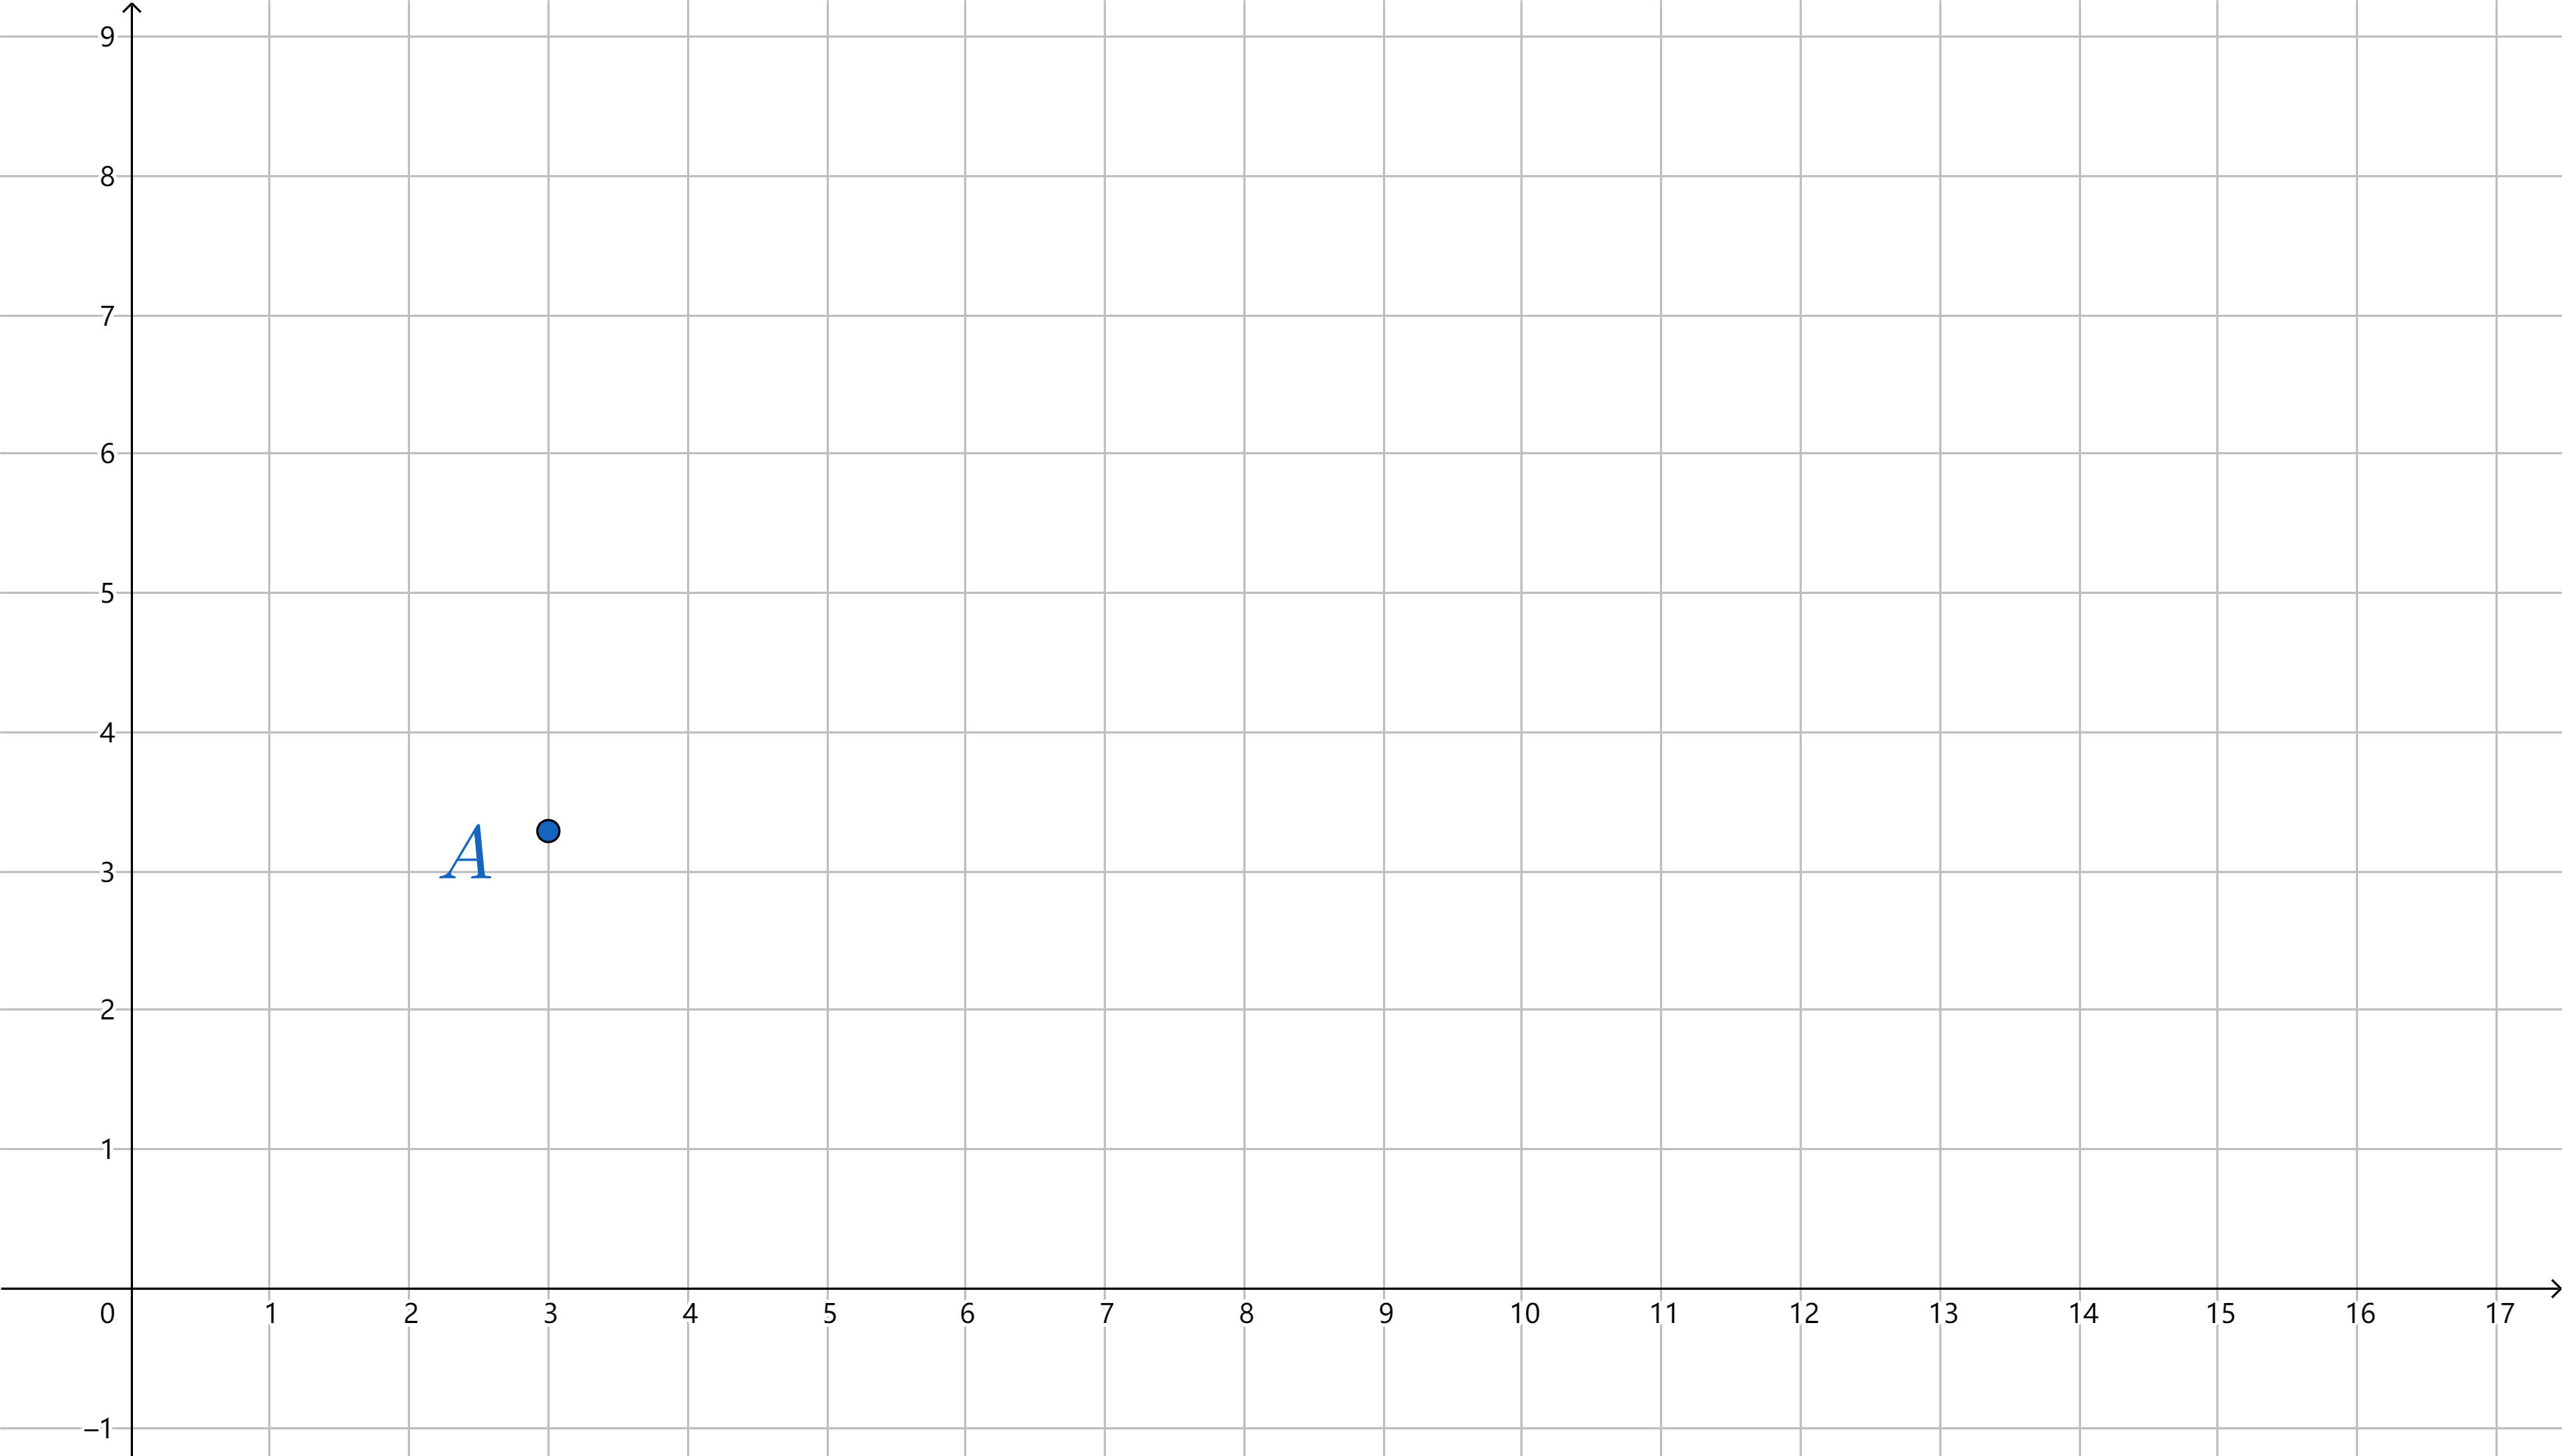
\includegraphics[width=5.76806in,height=3.27847in]{media/image14.png}

\textbf{【作图语句】}如下图,在 \(A\)
所在竖直格线的左侧第二条格线上取一个点 \(B\),将 \(B\)
向下平移两单位得到格点 \(B^{'}\),连 \(AB\) 交 \(A\)
所在竖直格线的左侧第一条格线于 \(C\),连接 \(B^{'}C\) 并延长交 \(A\)
所在竖直格线于 \(A^{'}\),\(A^{'}\) 即为所求。

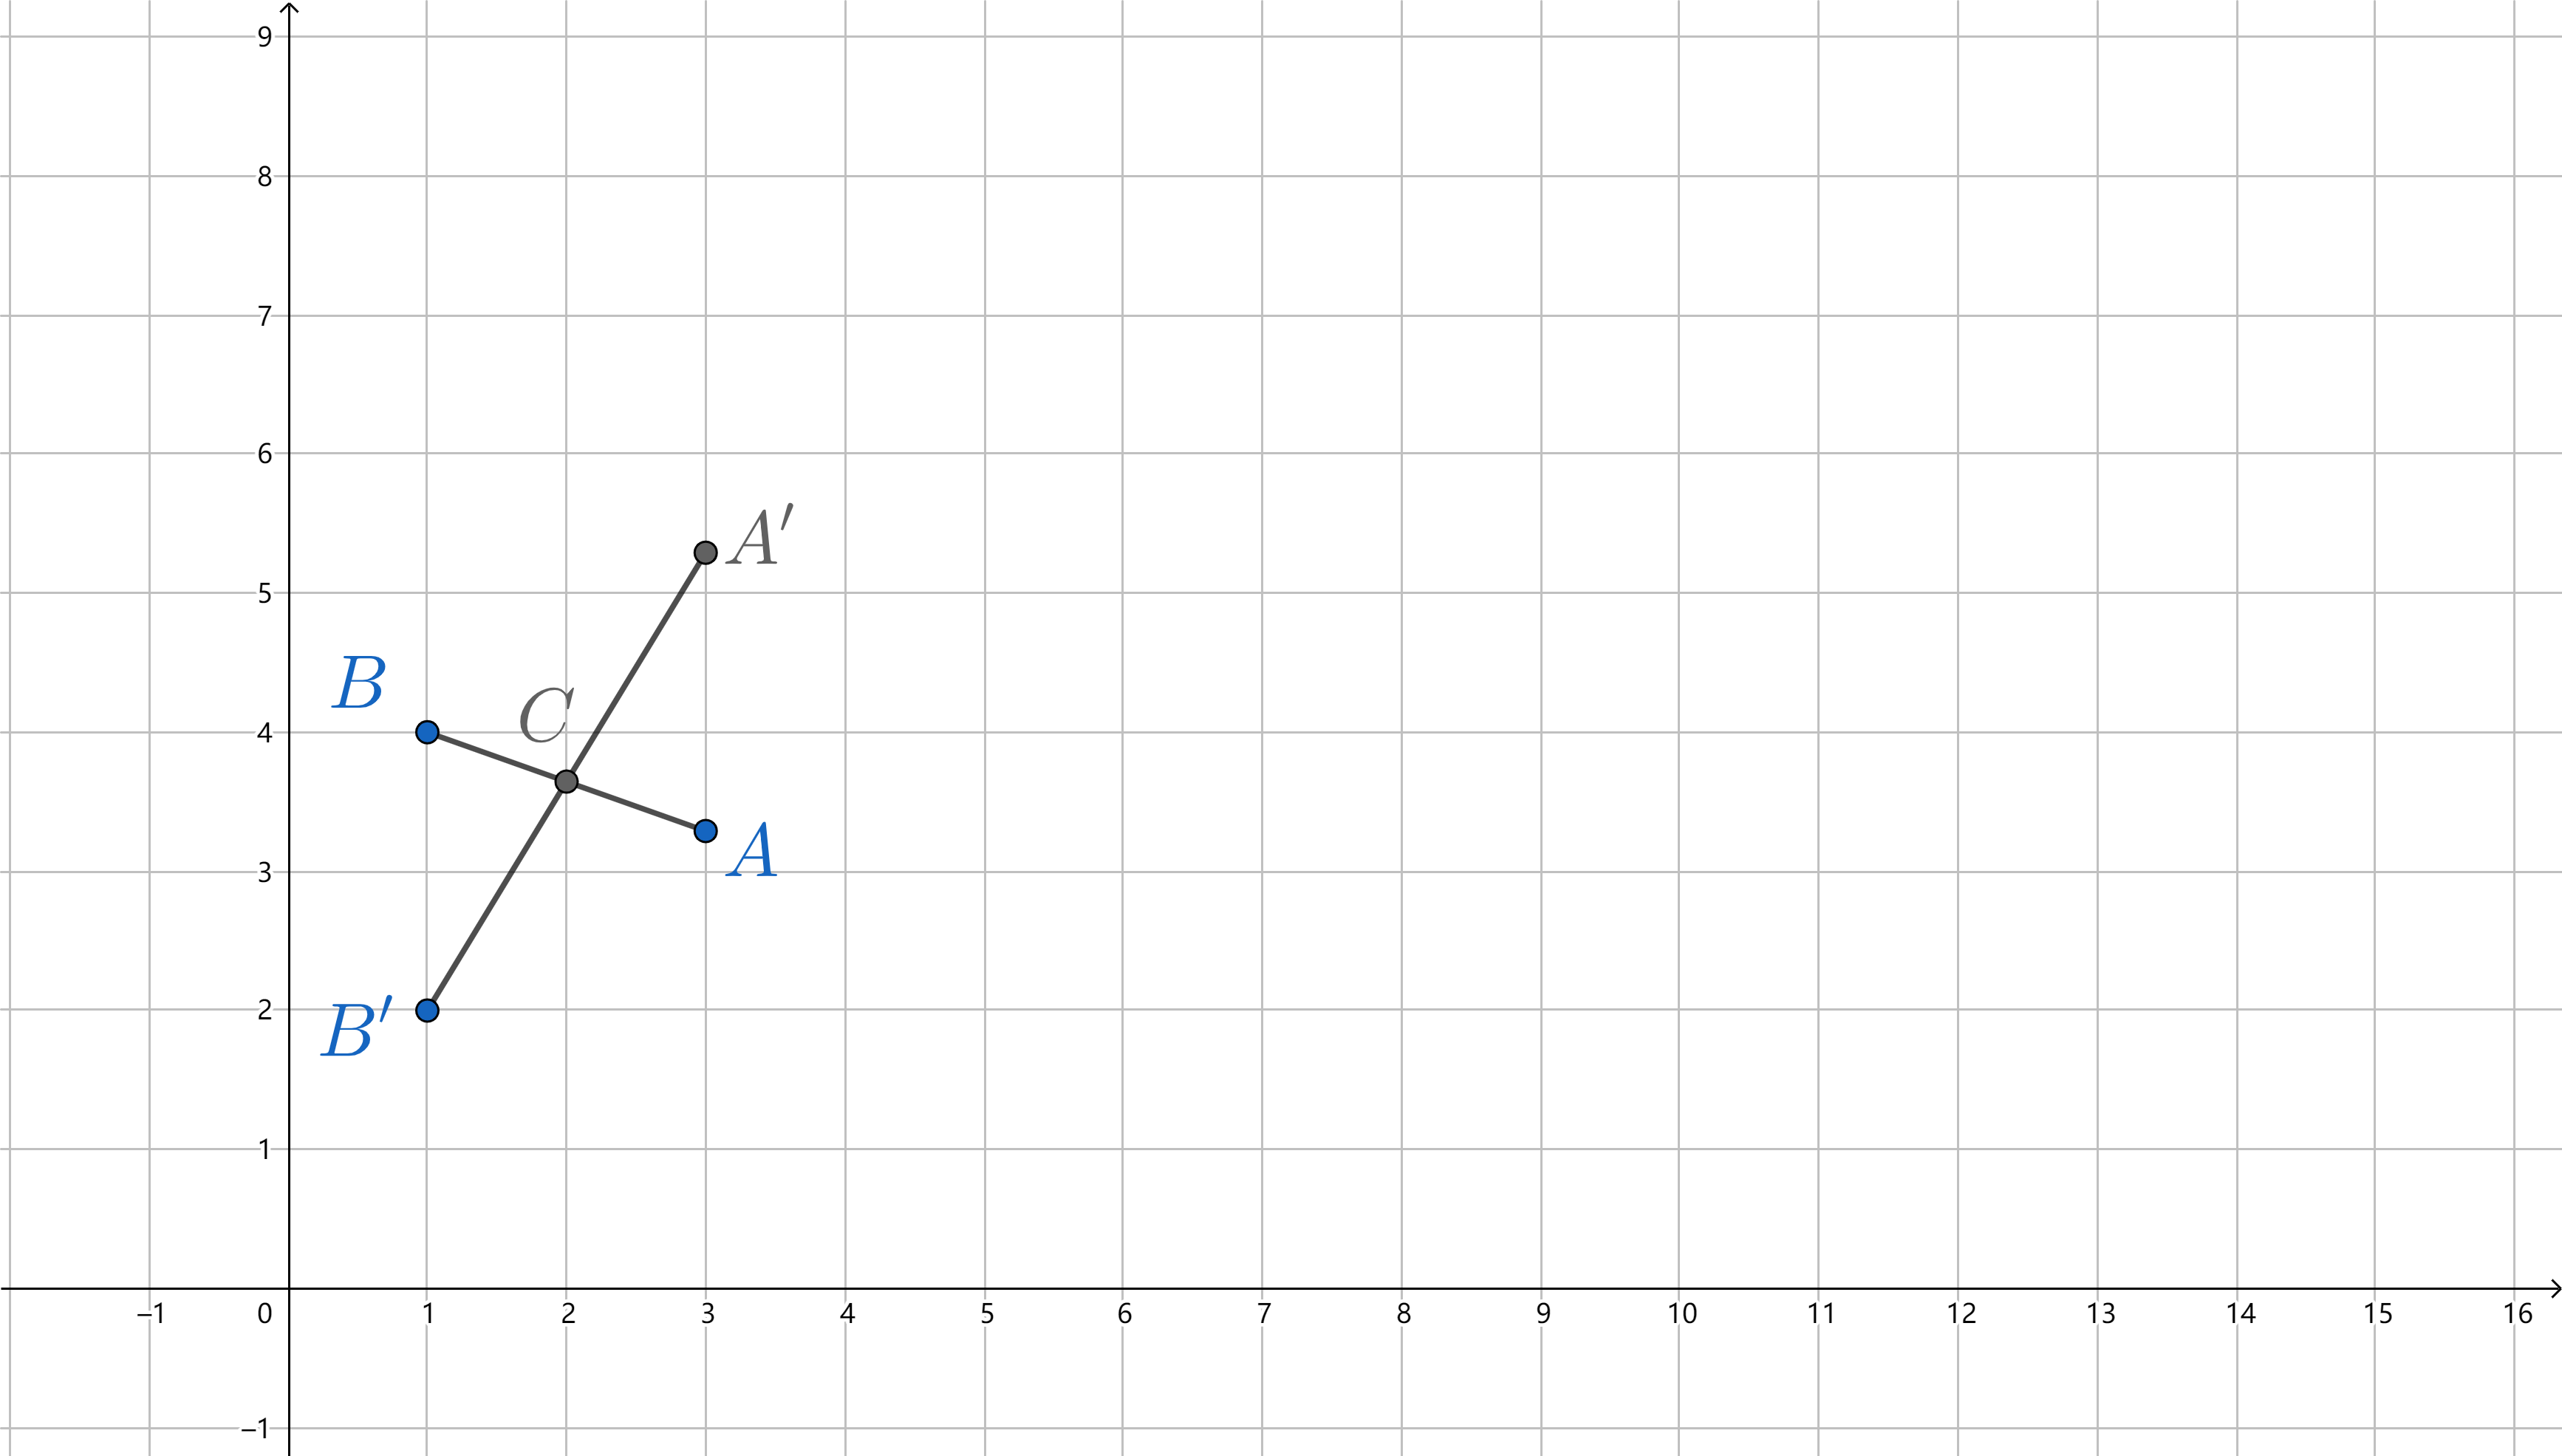
\includegraphics[width=5.76806in,height=3.27847in]{media/image15.png}

\textbf{【证明】}因为
\(CA = CB\),\(\angle BCB^{'} = \angle ACA^{'}\),\(CA^{'} = CB^{'}\),所以
\(\mathrm{\Delta}ACA^{'} \cong \mathrm{\Delta}BCB^{'}\),\(AA^{'} = BB^{'} = 2\)。

\textbf{跨格线平移}

如图,\(A\) 在竖直格线上,将其向右平移 \(n\left( n \in N^{*} \right)\)
个单位长度。下面将给出 \(n = 3\) 时的作图。

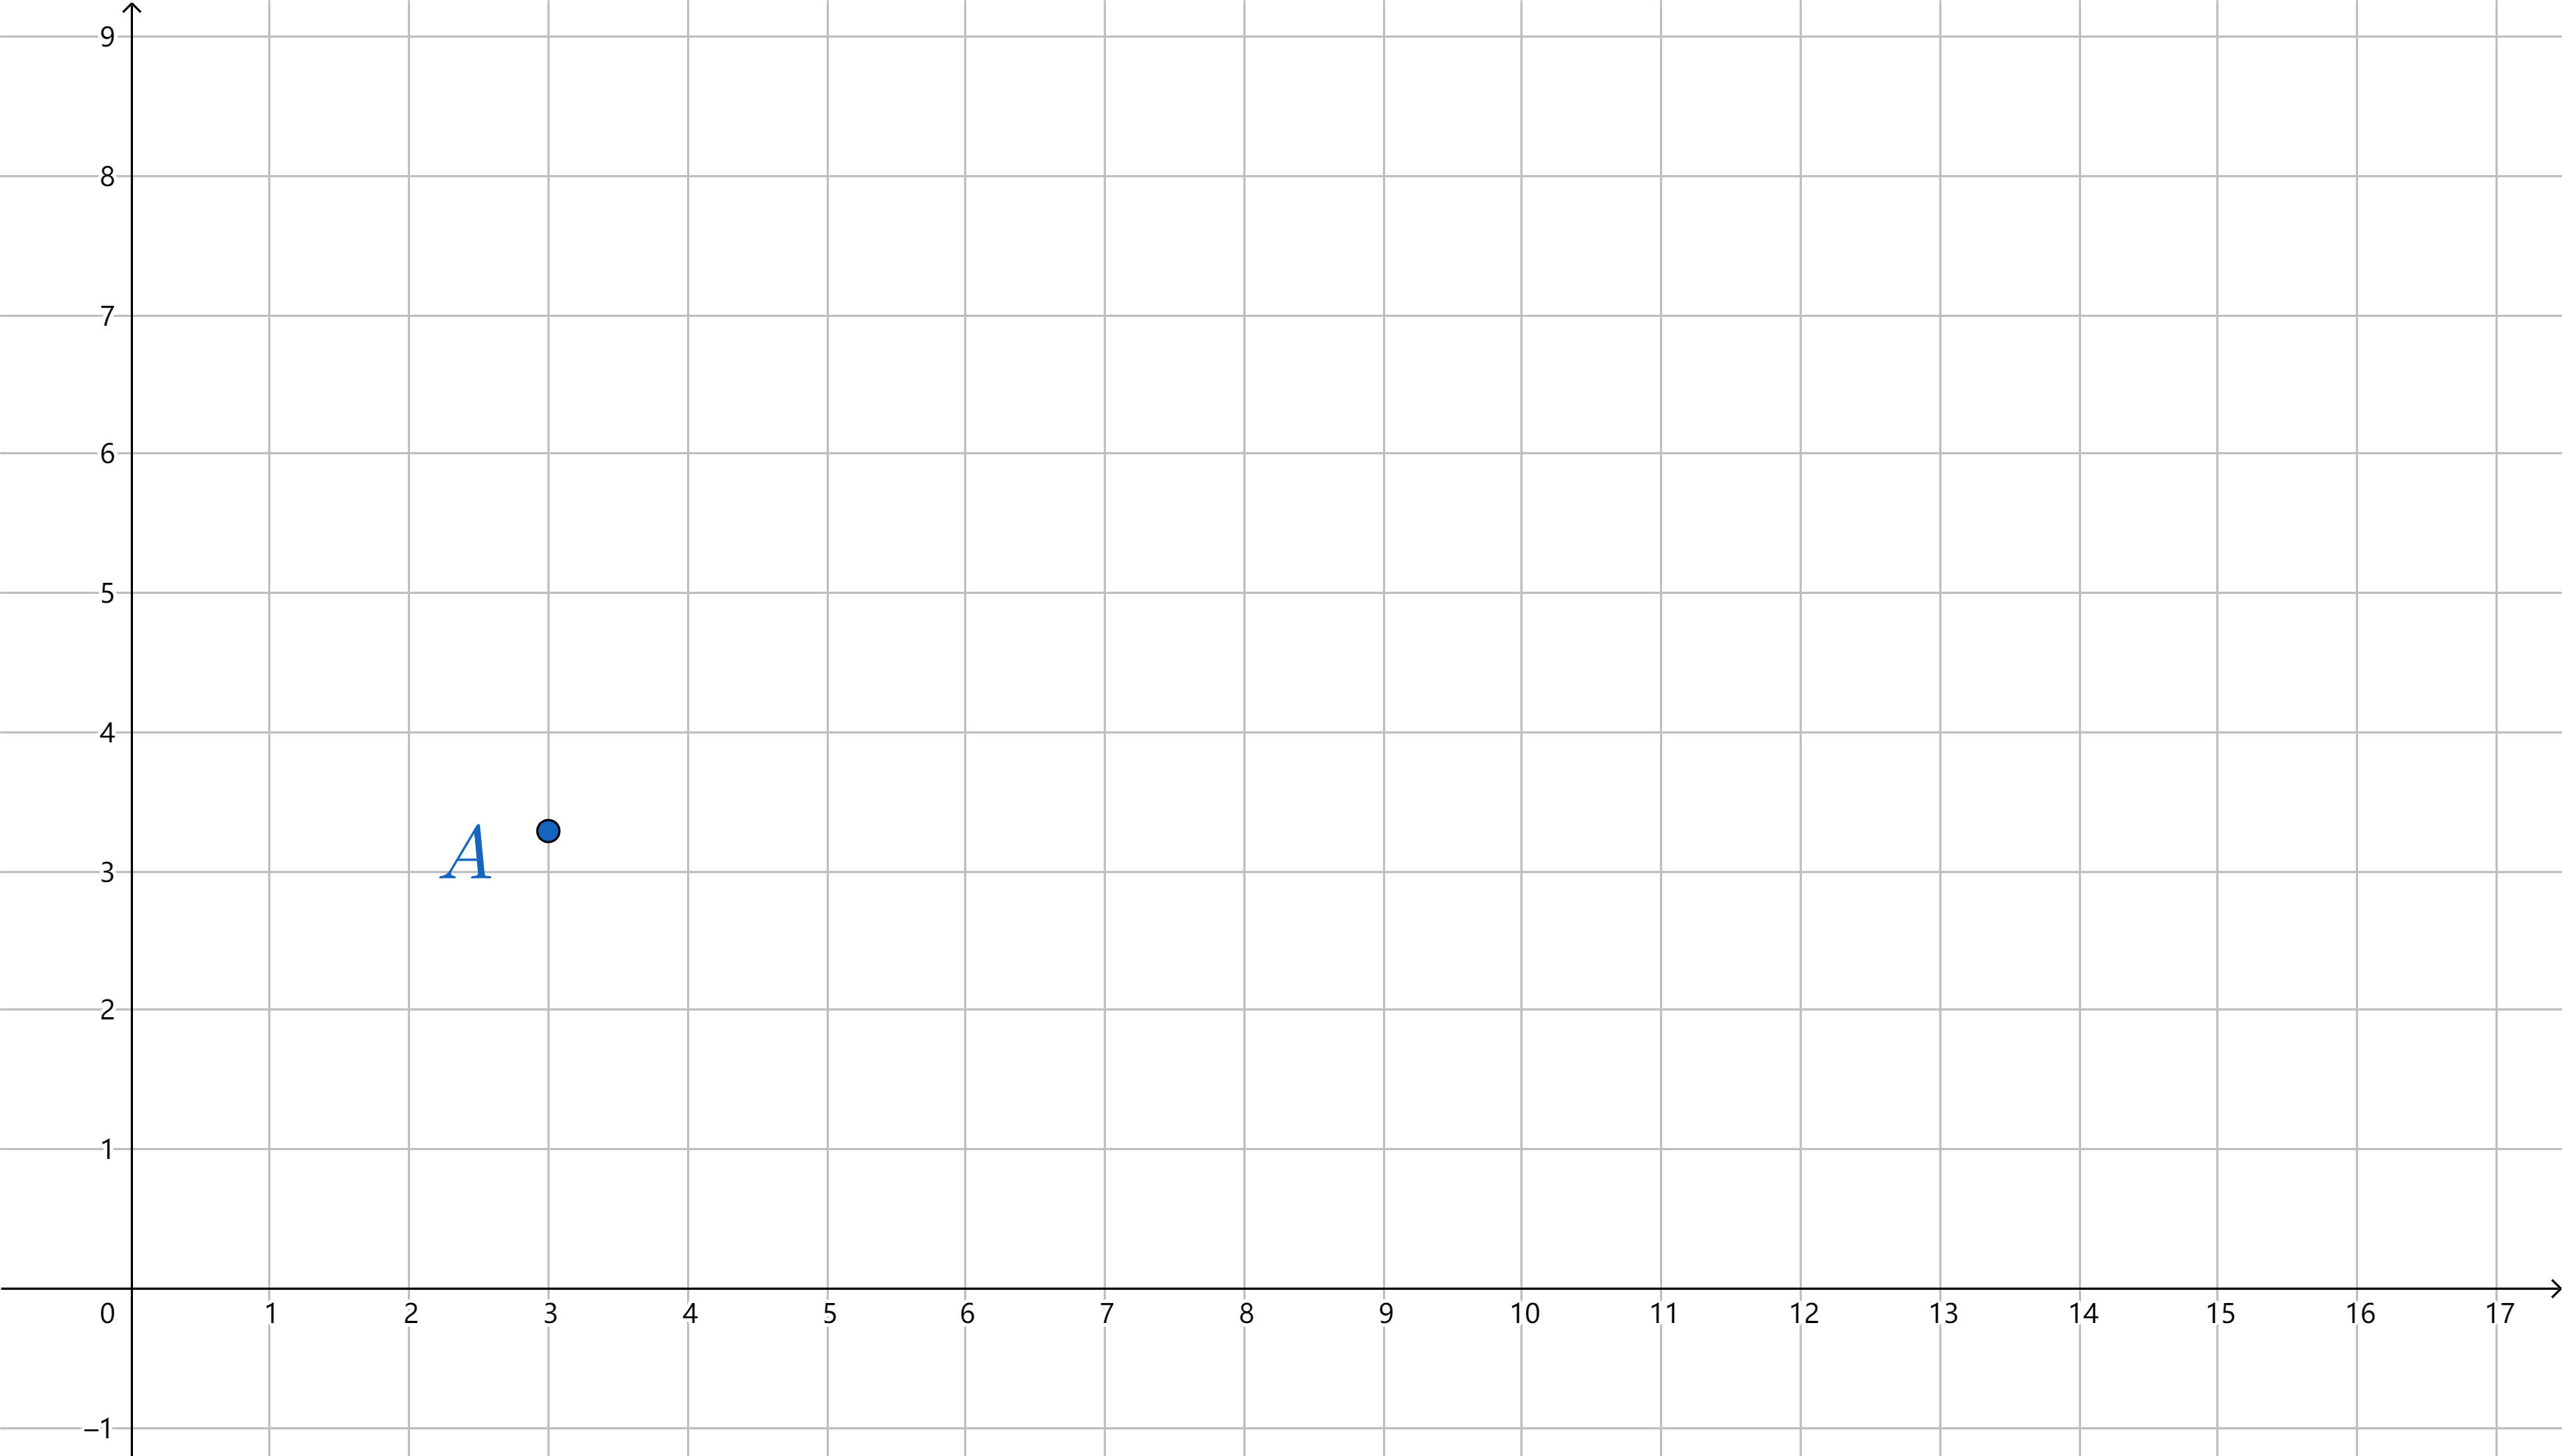
\includegraphics[width=5.76806in,height=3.27847in]{media/image14.png}

\textbf{【作图语句】}如下图,取格点 \(B\),\(B^{'}\),连 \(AB\)
交竖直格线于 \(C\),连 \(B^{'}C\) 并延长交竖直格线于 \(D\),连 \(AD\)
并延长交竖直格线于 \(A^{'}\),\(A^{'}\) 即为所求。

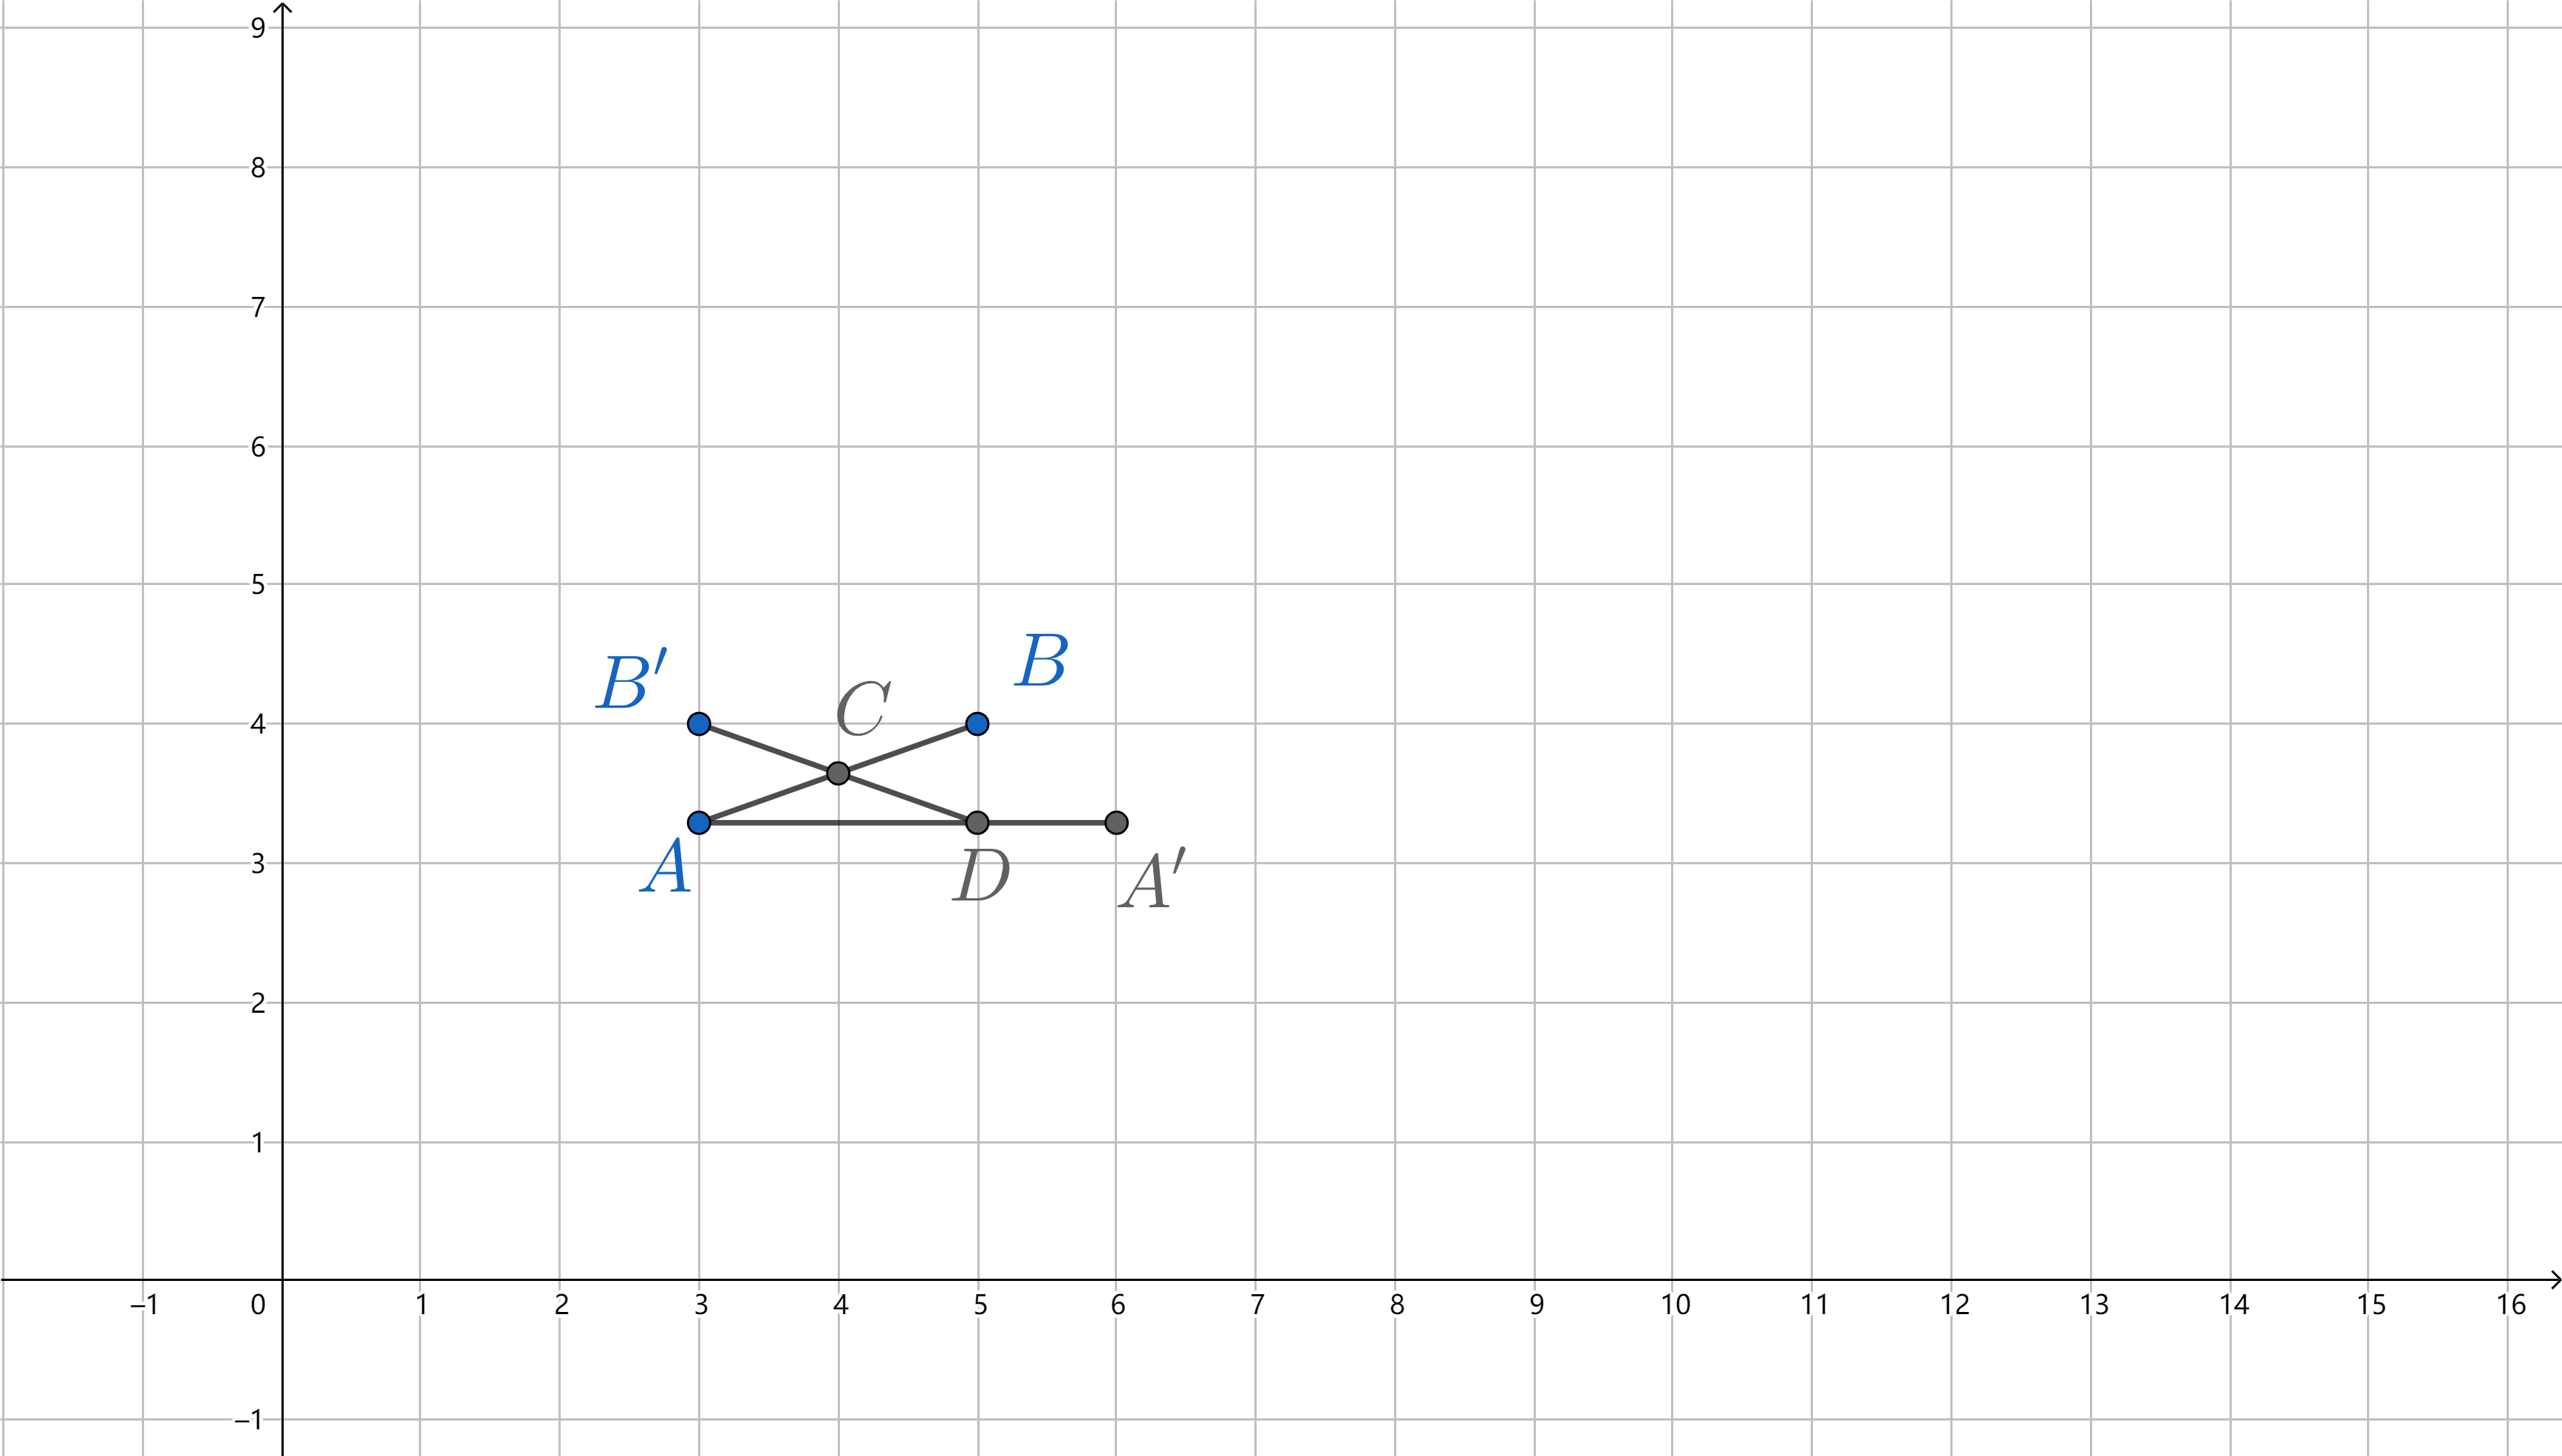
\includegraphics[width=5.76806in,height=3.27847in]{media/image16.png}

\textbf{【证明】}因为 \(CA = CB = CB^{'} = CD\),所以四边形 \(AB^{'}BD\)
是矩形,\(AA^{'} \parallel BB^{'}\),结论得证。

\subsection{2.
分线段与倍长}

\hypertarget{wycux4e24ux5927ux5206ux7ebfux6bb5ux5b9aux7406}{%
\subsubsection{Wyc两大分线段定理}\label{wycux4e24ux5927ux5206ux7ebfux6bb5ux5b9aux7406}}

在讨论将一条线段分成给定比例之前,我们先考虑如何平分它。虽然平分线段定理(定理
3.1.2)给出了做法,但是过程太过于复杂,我们需要考虑在一些特殊情况下可不可以简化一些步骤,然后再尝试推广到更一般的情况。

Wyc同学考虑了一个很好的特殊情况------当线段的一个端点在格线上。如下图所示,\(A\)
在格线上,我们需要平分线段 \(AB\)。

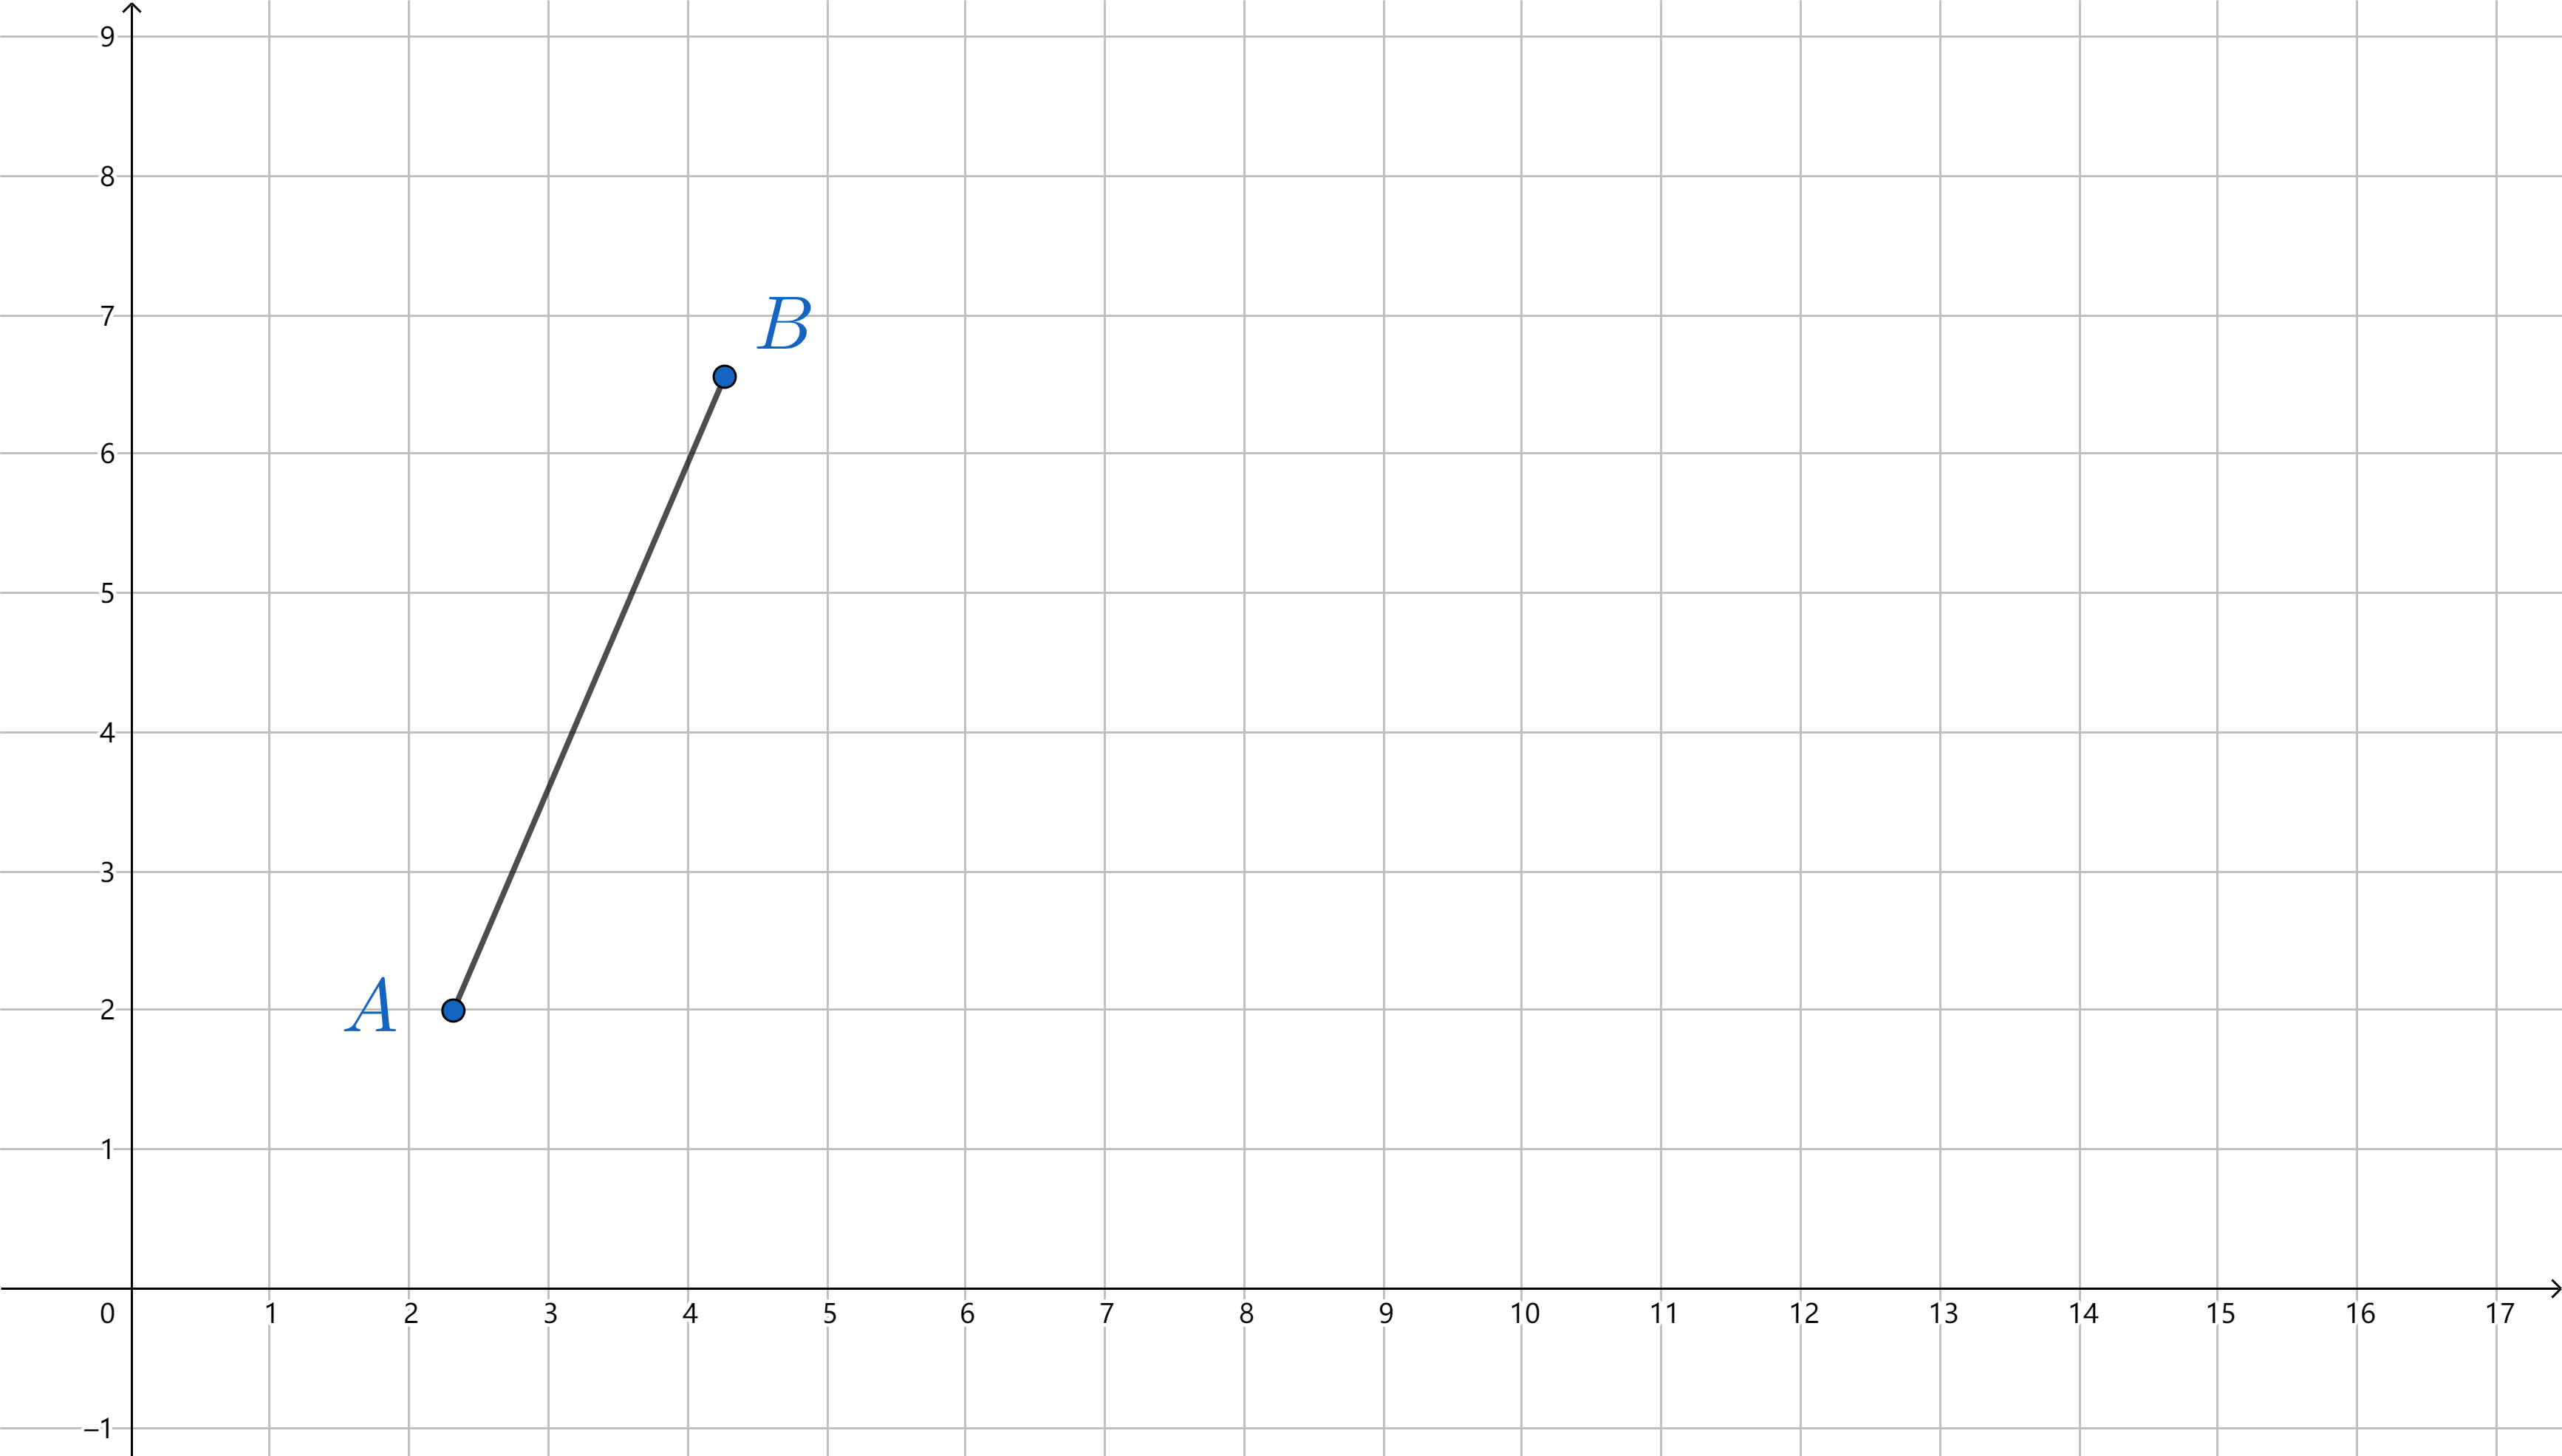
\includegraphics[width=5.76806in,height=3.27847in]{media/image17.png}

Wyc通过构造中位线的方法解决了这个问题。首先我们过 \(B\)
随便画一条合适的直线。

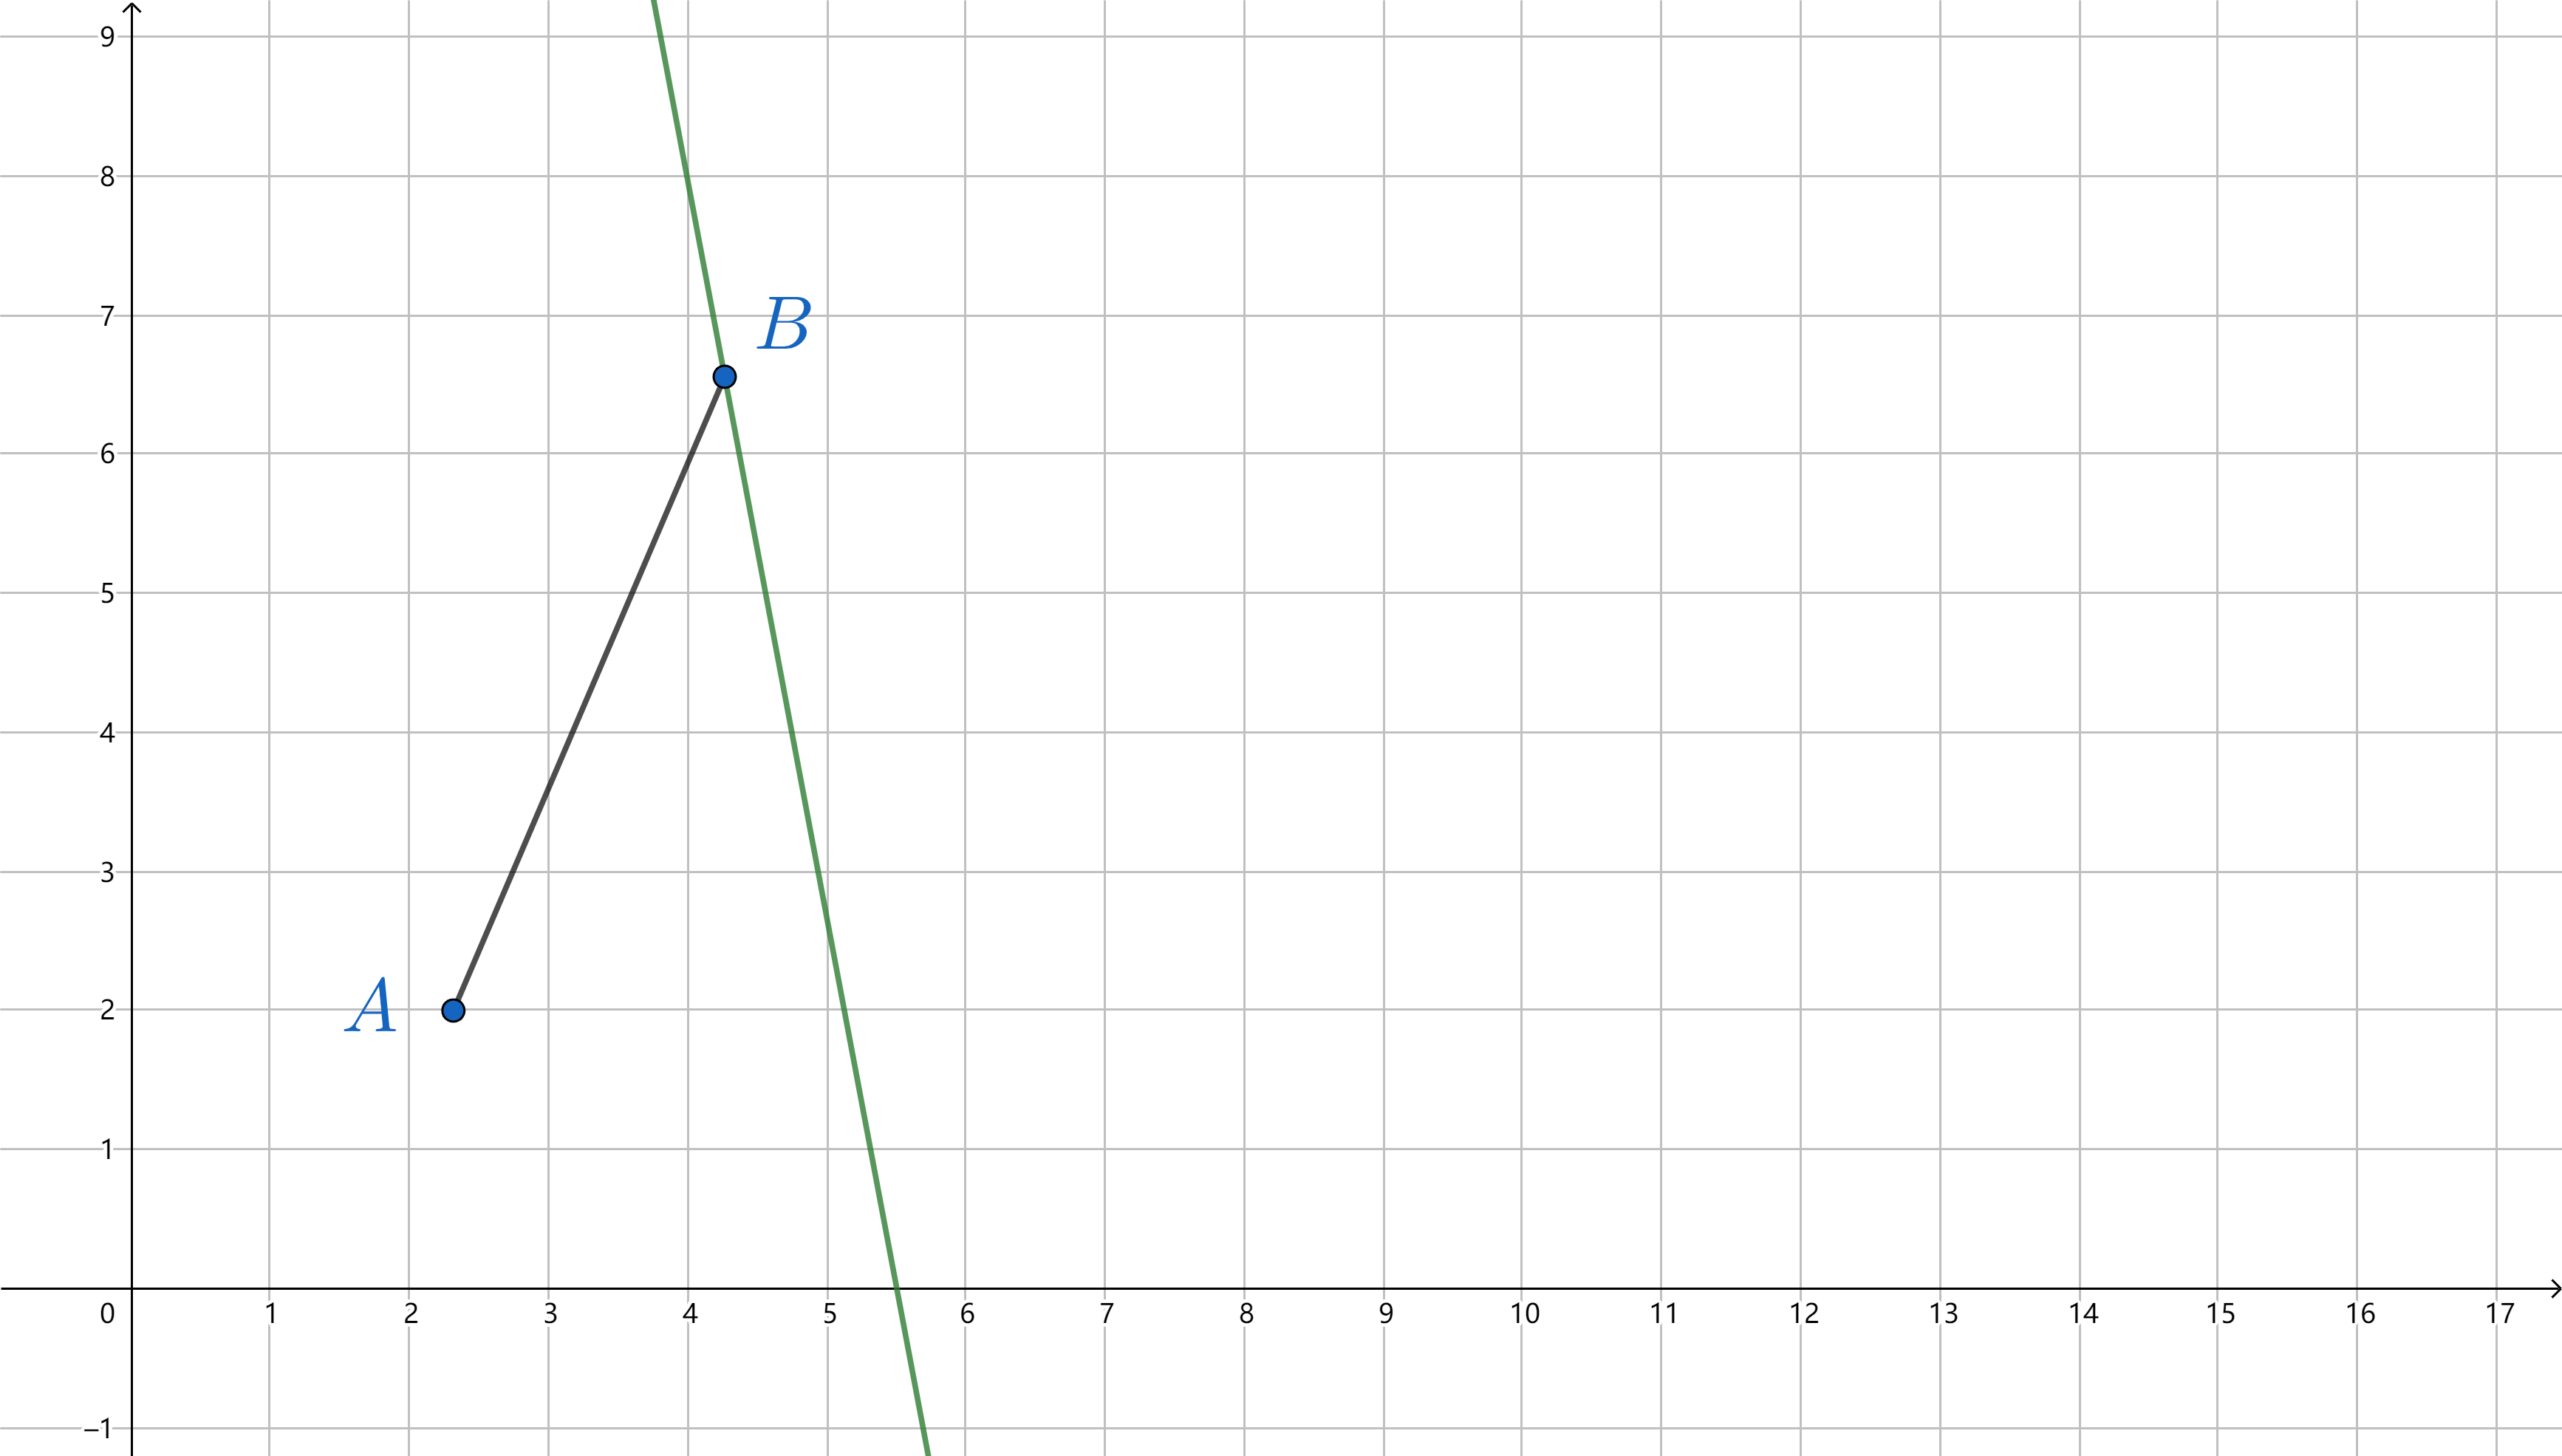
\includegraphics[width=5.76806in,height=3.27847in]{media/image18.png}

我们找到这条直线与两条水平格线的交点,设为 \(C\),\(D\)。

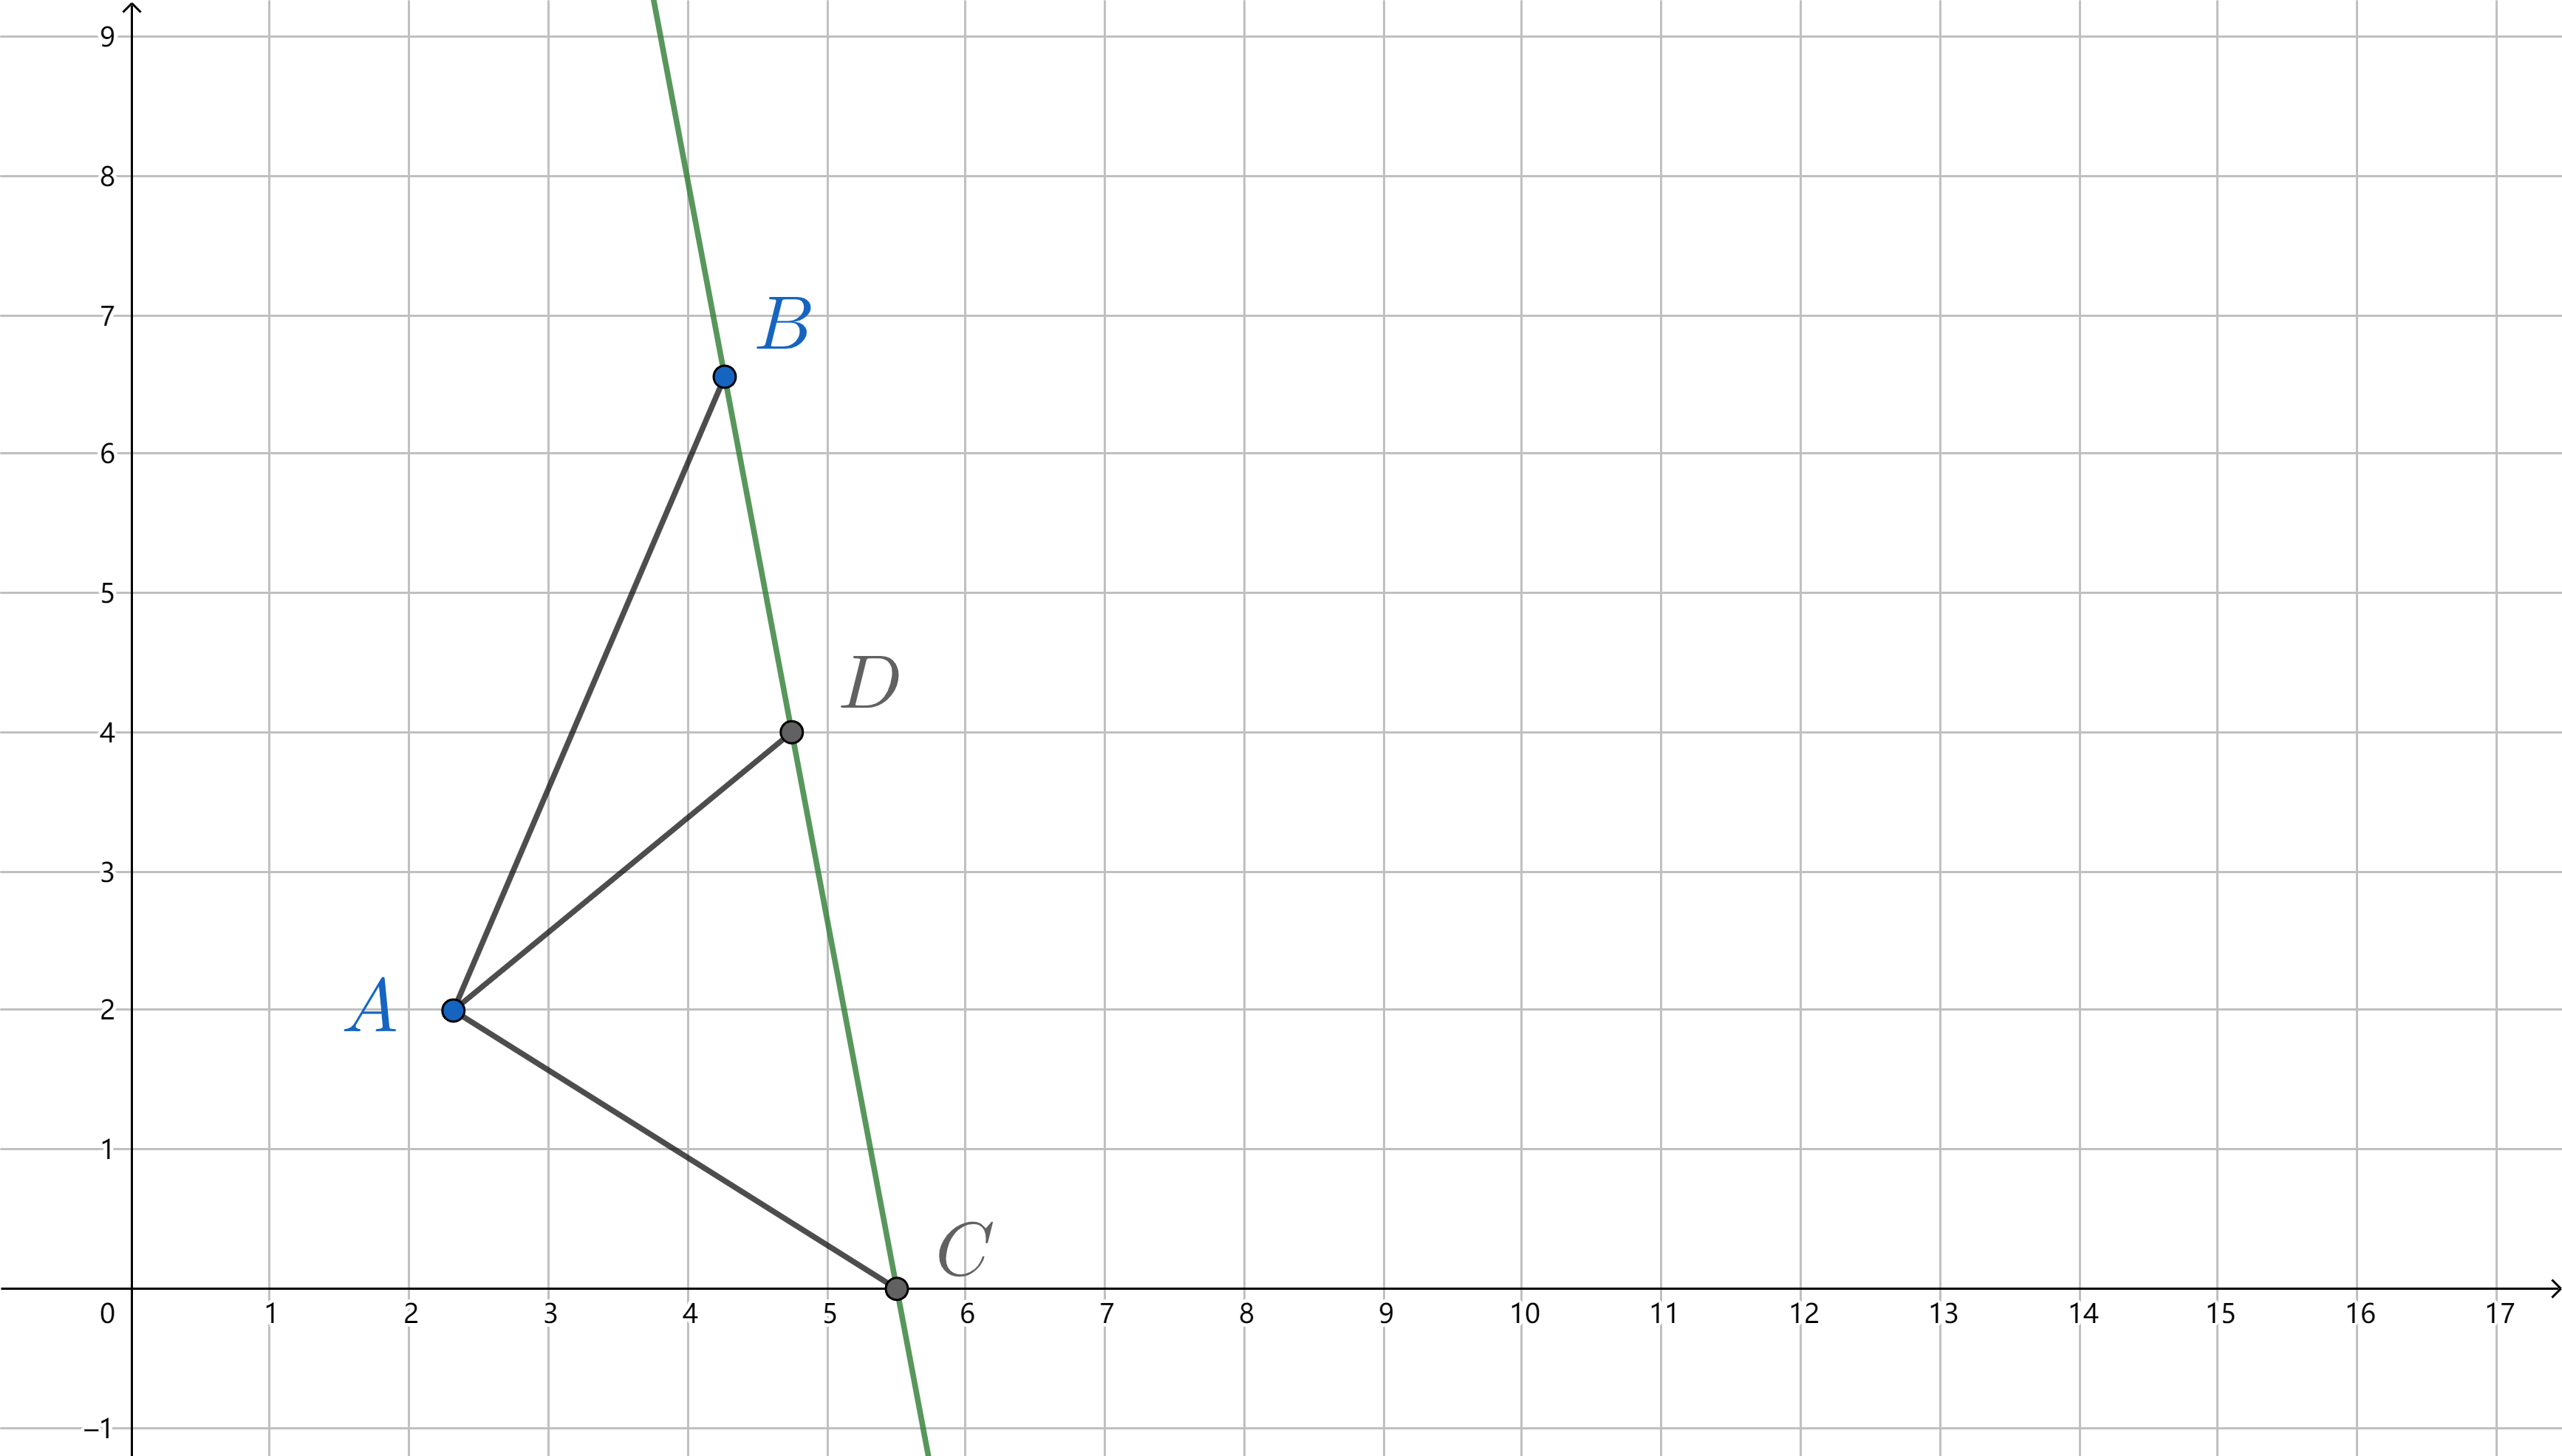
\includegraphics[width=5.76806in,height=3.27847in]{media/image19.png}

我们可以利用 ``\(A\) 在格线上'' 这一条件来简单地画出 \(AD\),\(AC\)
的中点。显然,线段 \(AD\) 与 \(A\)、\(D\) 中间水平格线的交点就是 \(AD\)
的中点,线段 \(AC\) 与 \(A\)、\(C\) 中间水平格线的交点就是 \(AC\)
的中点。

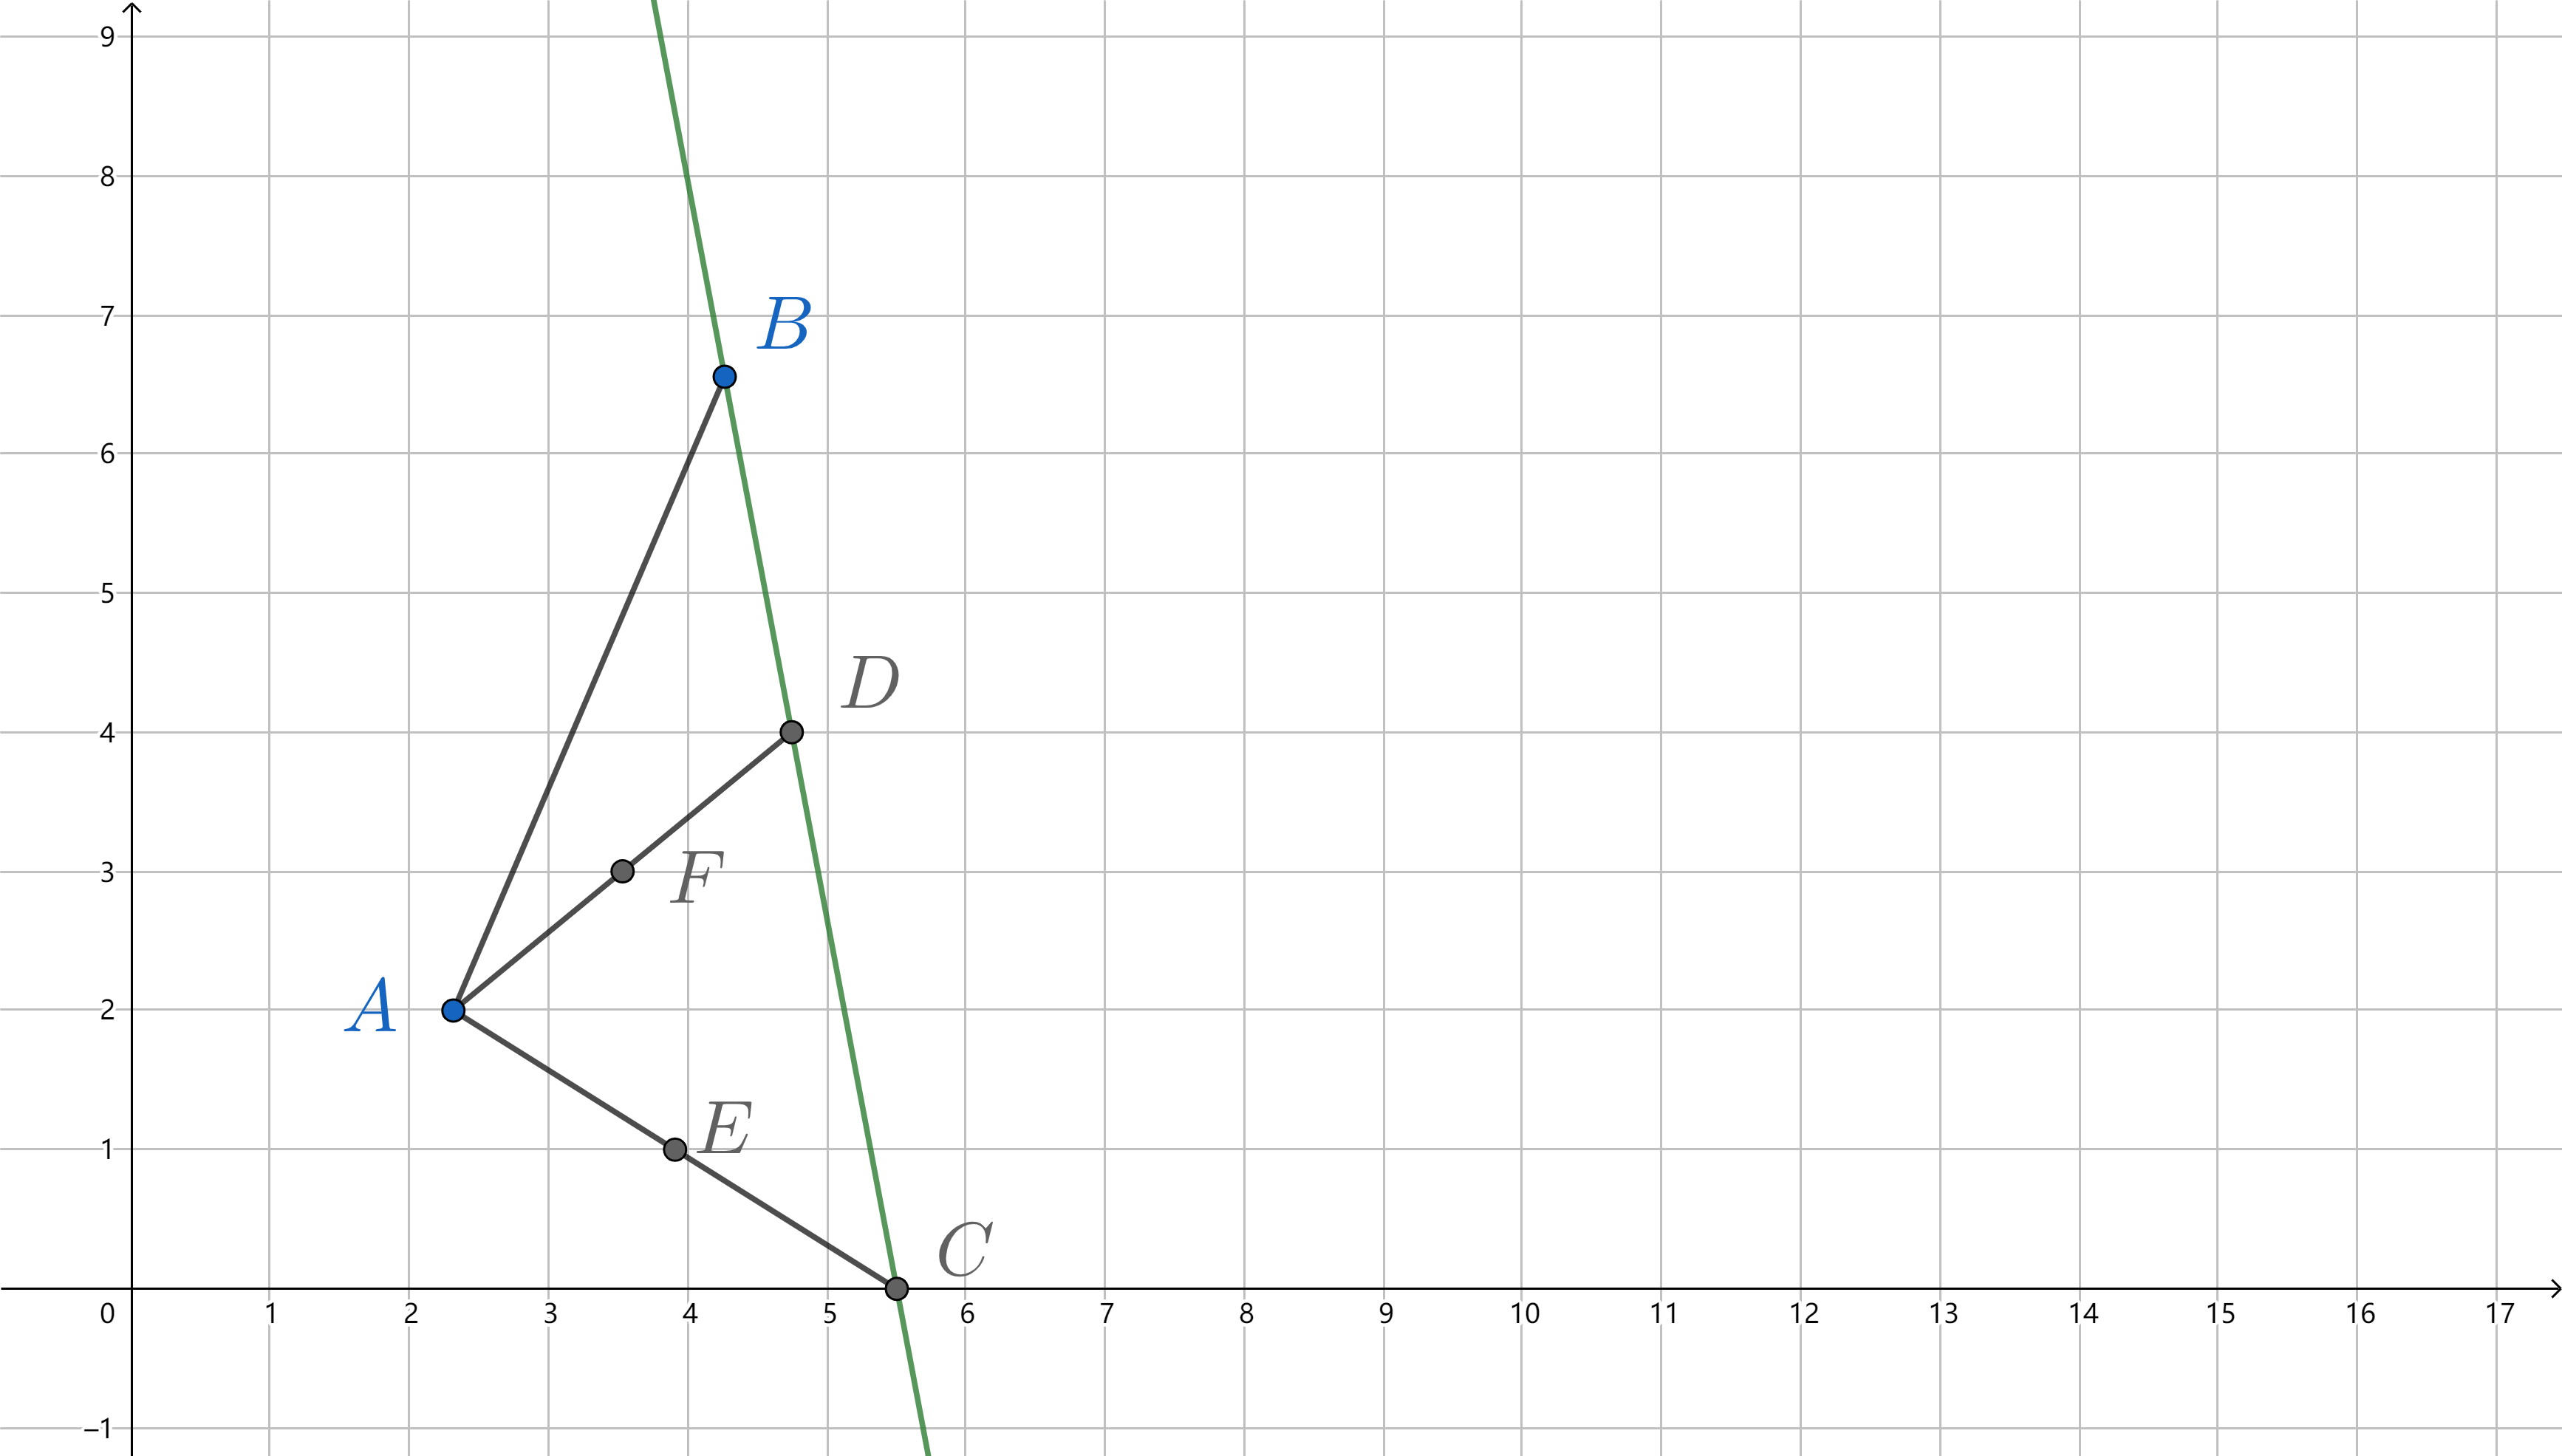
\includegraphics[width=5.76806in,height=3.27847in]{media/image20.png}

连接 \(EF\) 并延长交 \(AB\) 于 \(M\),\(M\)
即为所求。它的正确性是显然的,这里就不提供证明了。

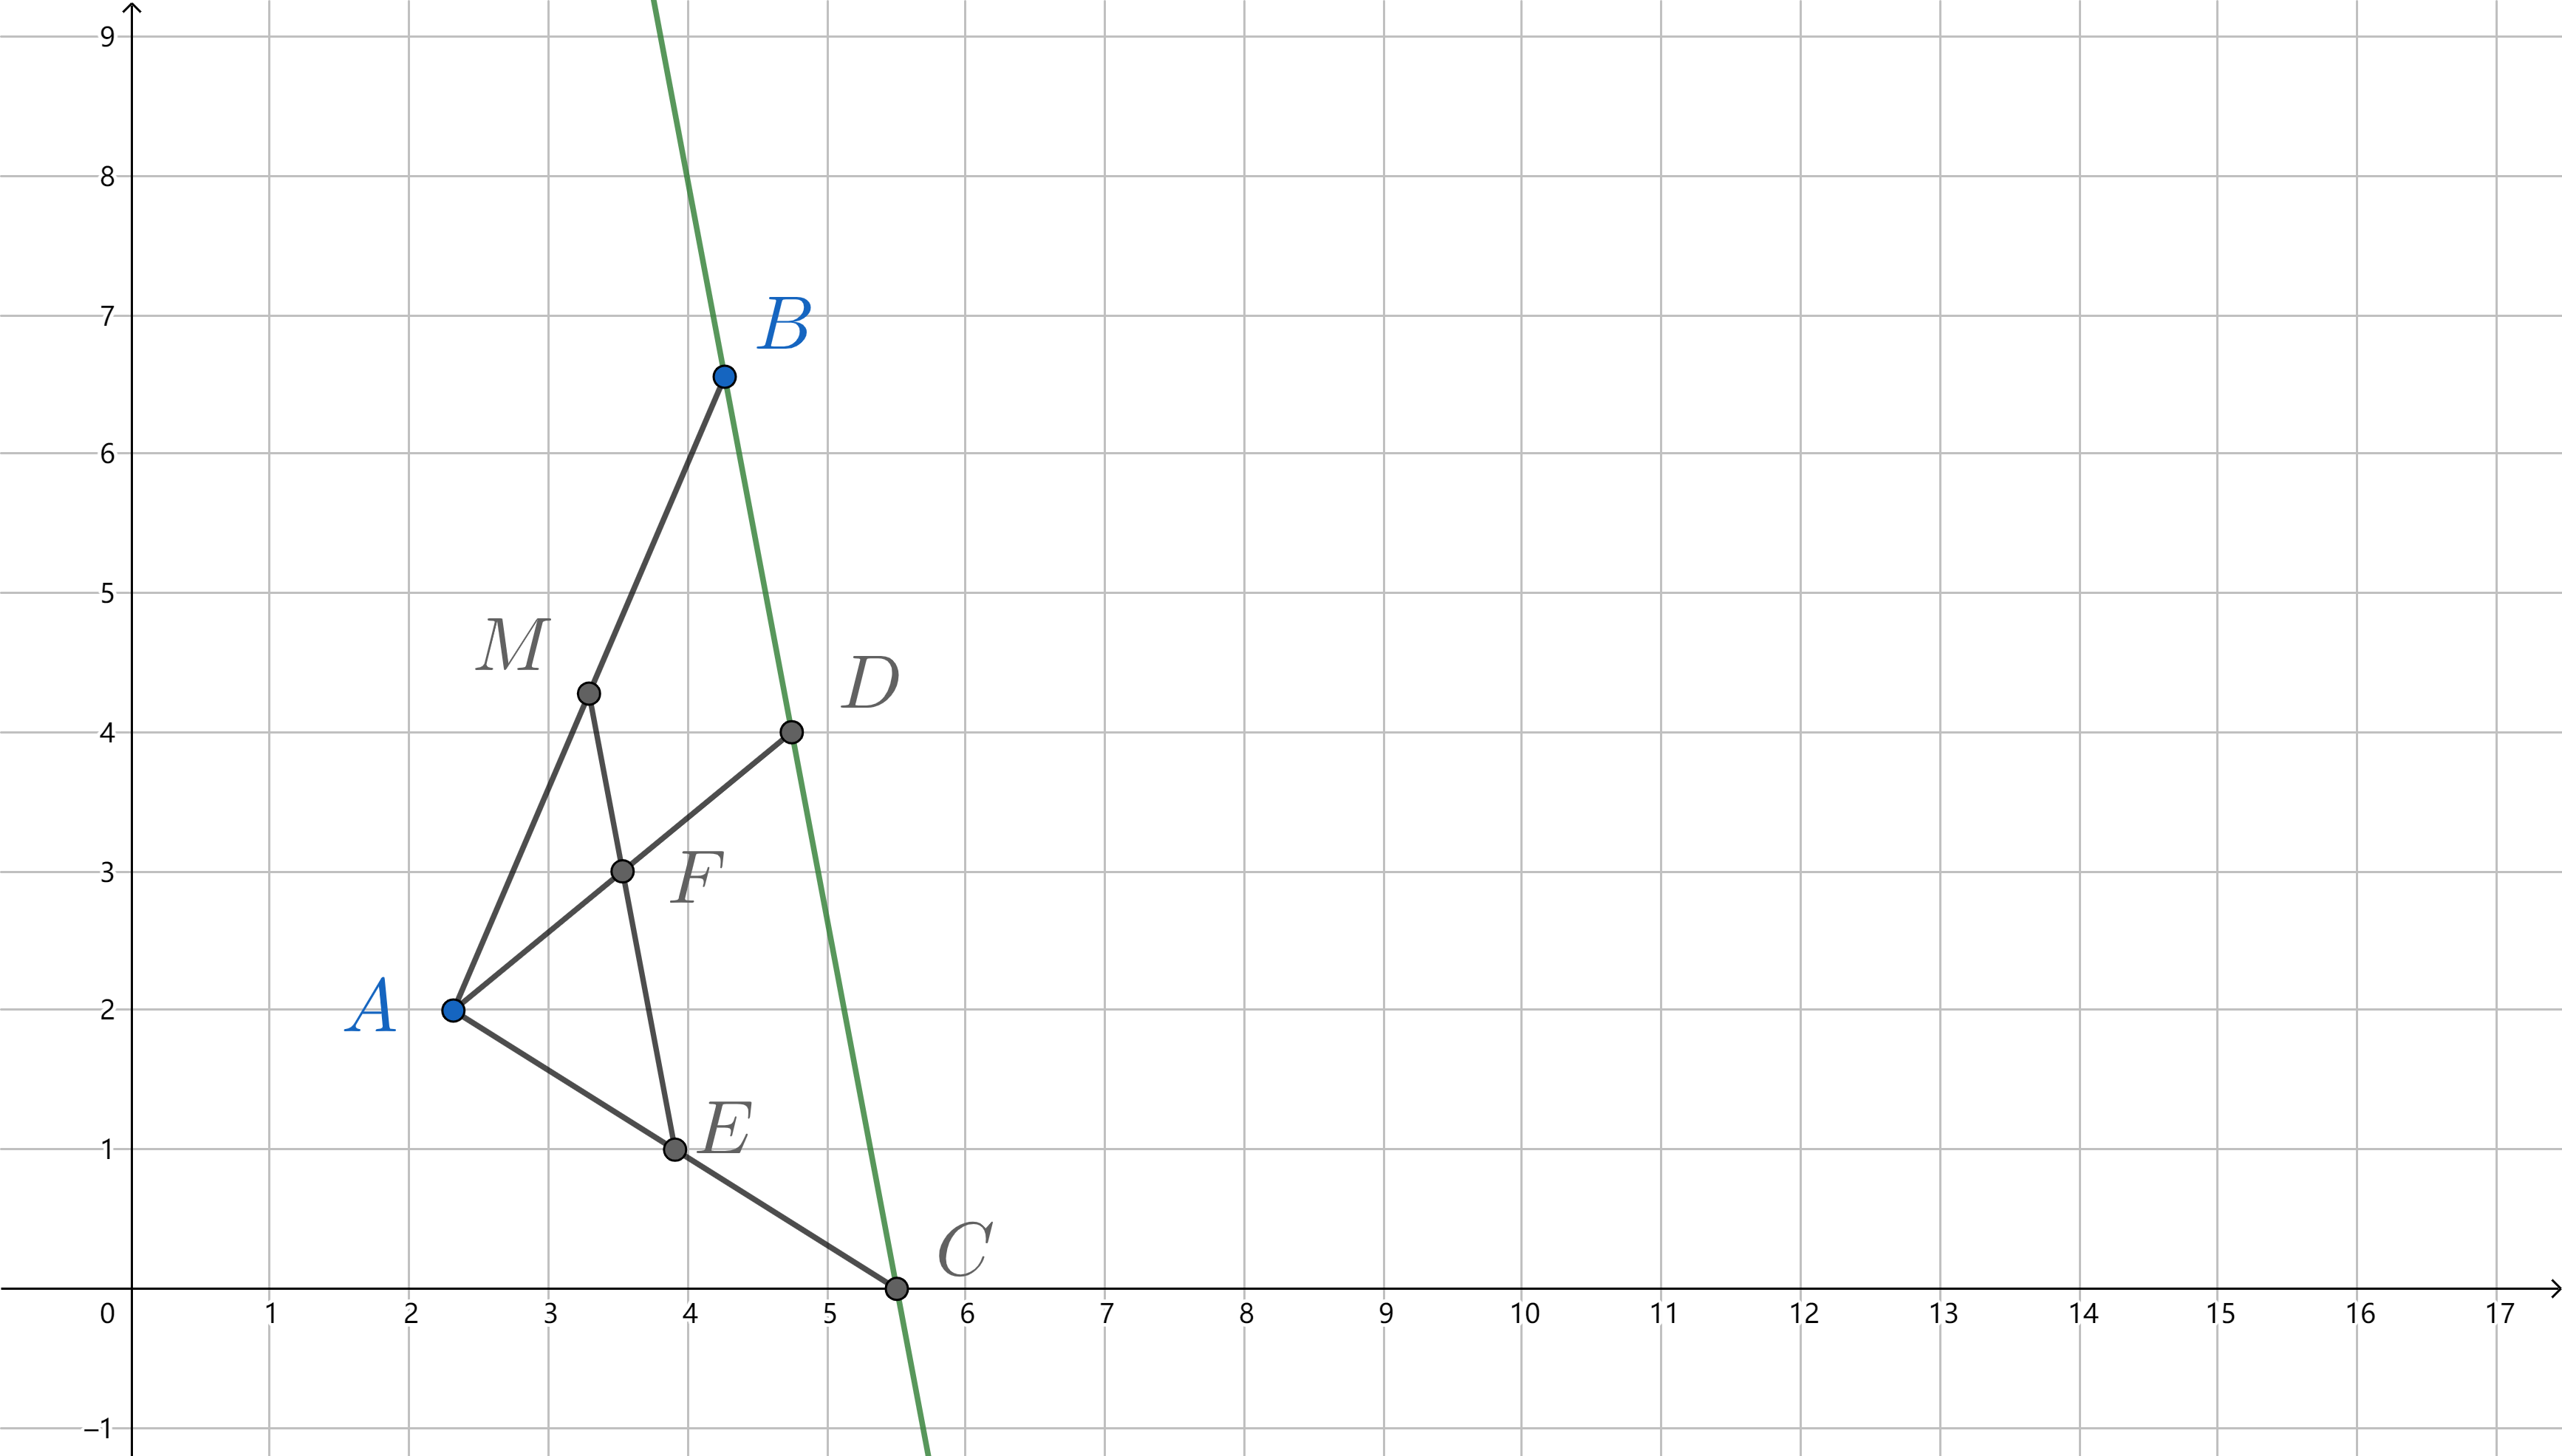
\includegraphics[width=5.76806in,height=3.27847in]{media/image21.png}

\textbf{【拓展】}我们可以用很相似的方法作出一条线段(一端点在格线上)的三等分点、四等分点以及其他比例的分线段点。下面的图给出了作三等分点的方法:

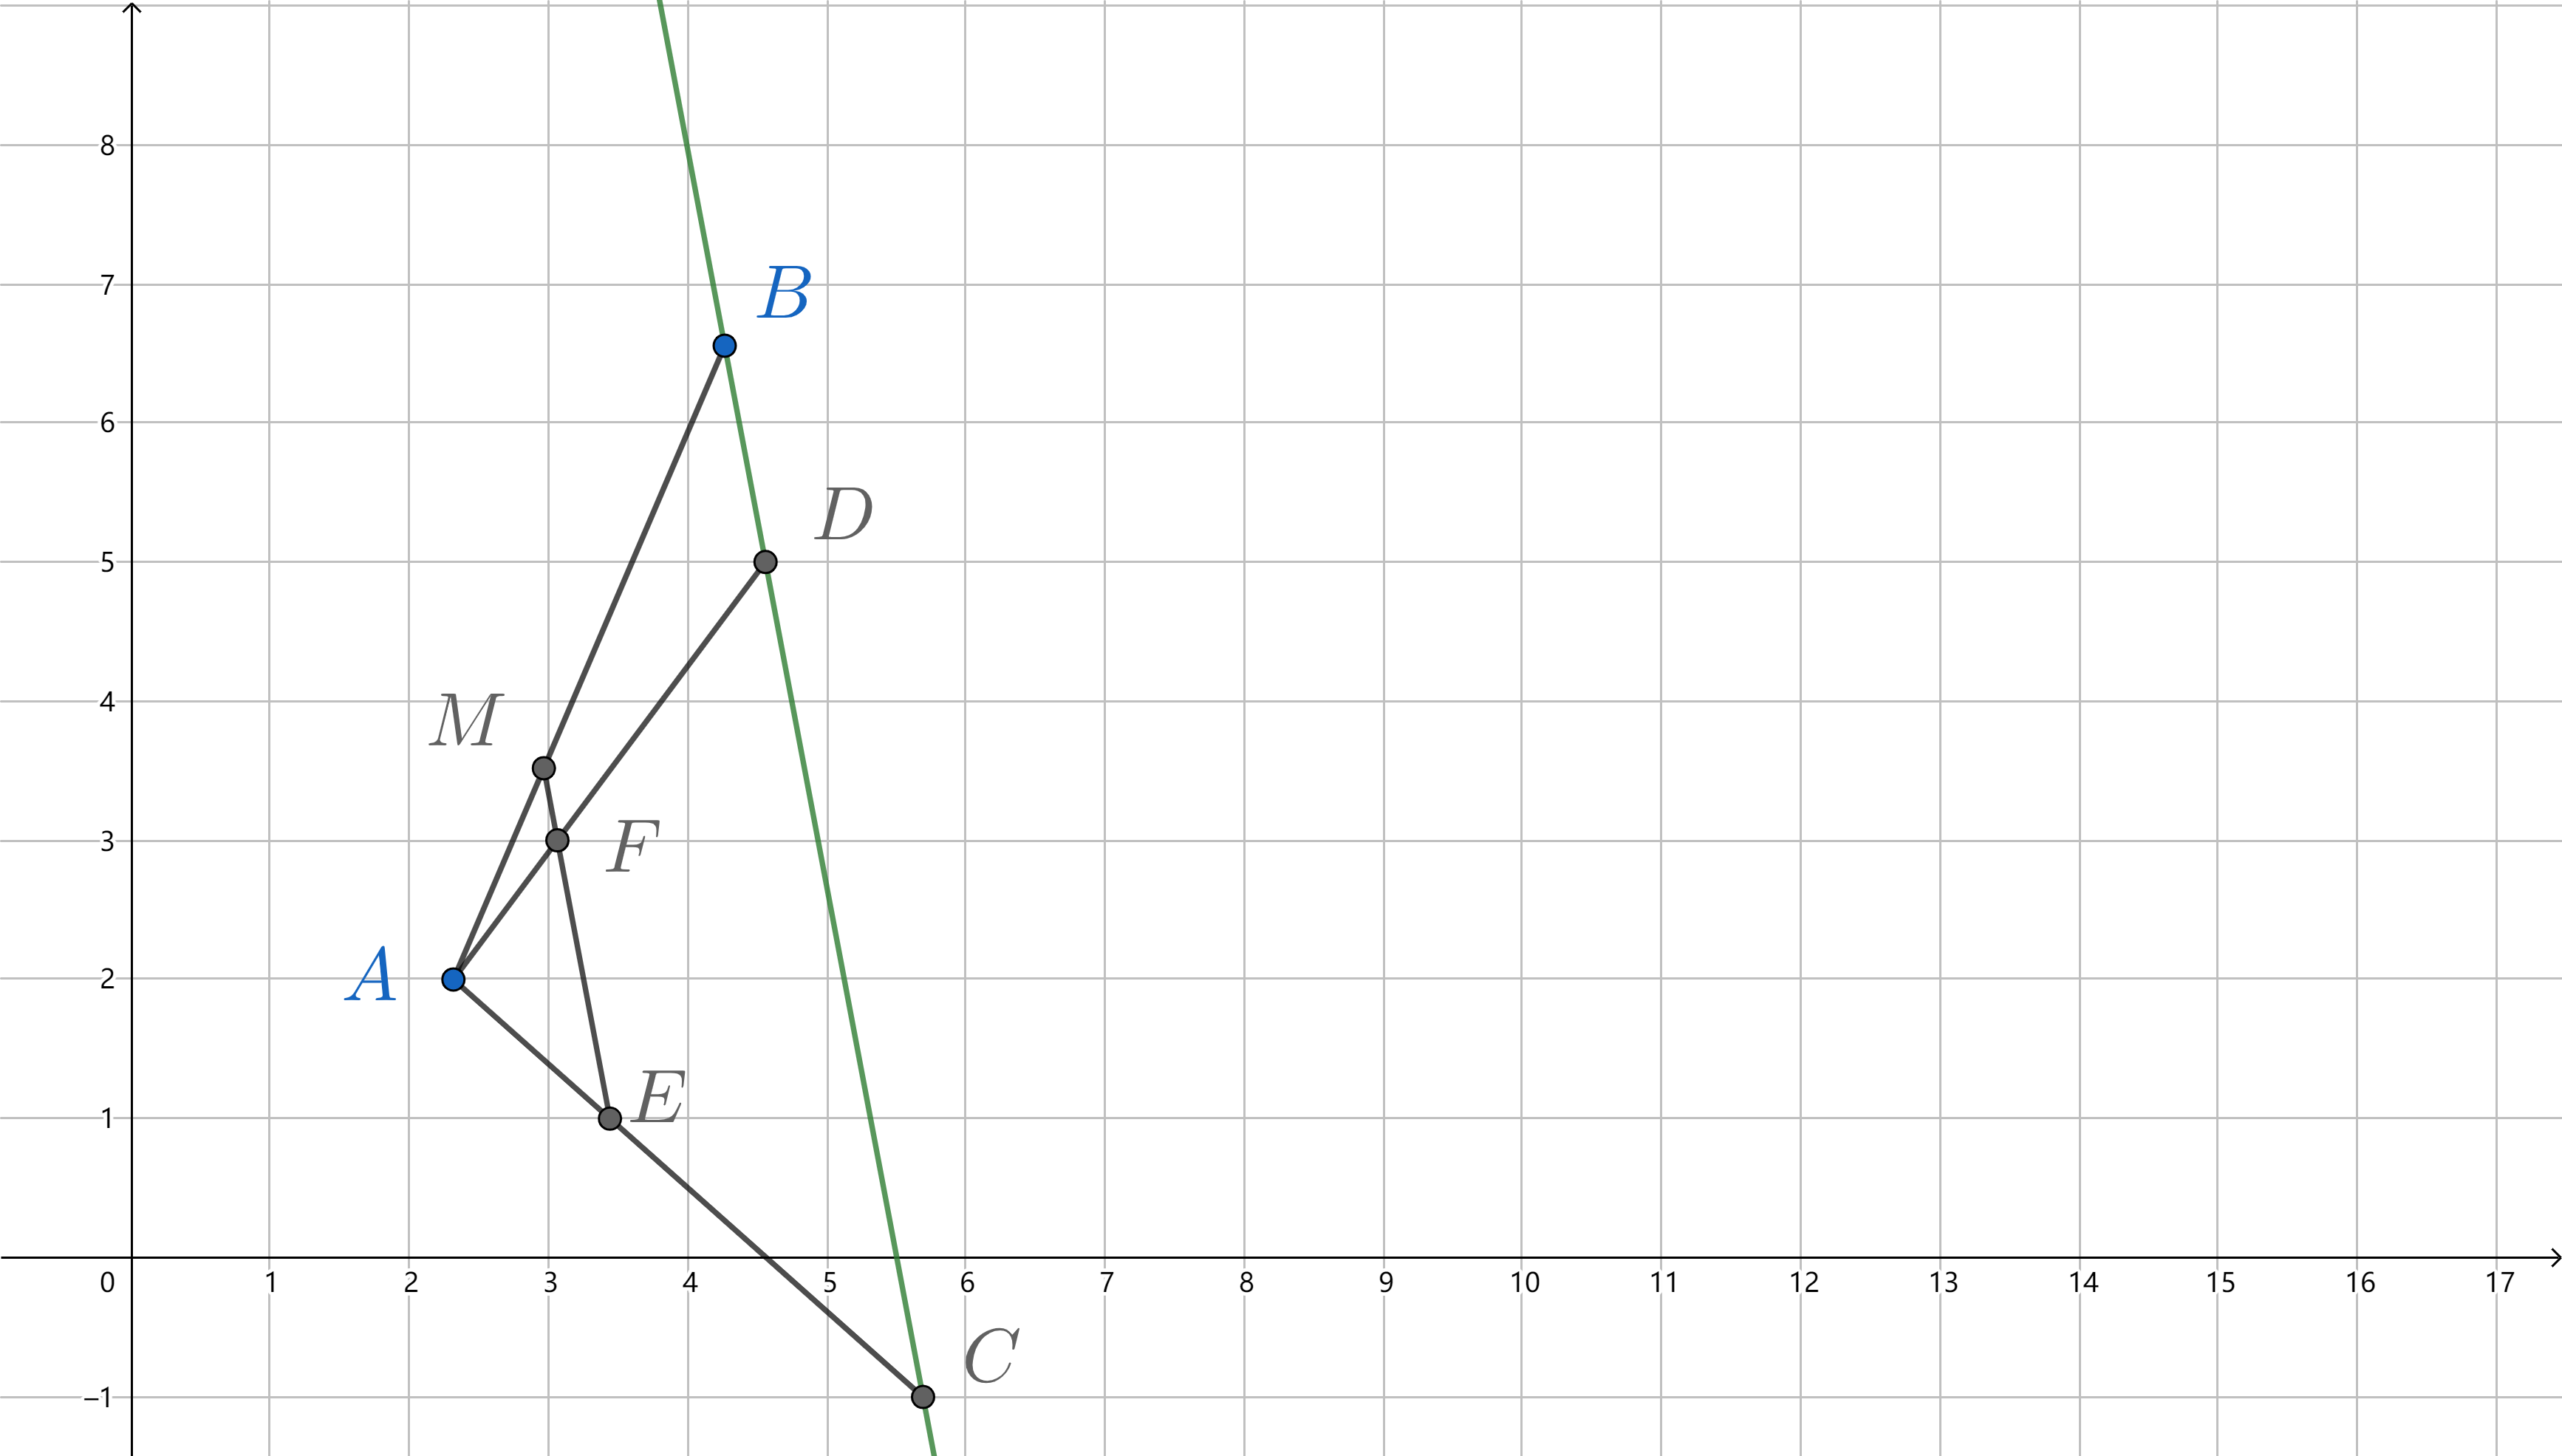
\includegraphics[width=5.76806in,height=3.27847in]{media/image22.png}

Wyc分线段定理的思路,可以用概括为如下的部分。首先,当一条线段的两个端点都在格线上,且这两条格线都是水平格线或都是竖直格线的时候,这条线段的中点很好作;我们可以利用这个特点,构造中位线或相似,解决比较一般的情况。

\hypertarget{wycux5206ux7ebfux6bb5ux5b9aux7406-wycs-segment-dividing-theoremux5b9aux7406-3.4}{%
\subsection{Wyc分线段定理 Wyc's Segment Dividing Theorem(定理
3.4)}\label{wycux5206ux7ebfux6bb5ux5b9aux7406-wycs-segment-dividing-theoremux5b9aux7406-3.4}}

\textbf{【提出者】}王宇辰

当一条线段的一个端点在格线上时,可以用比平分线段定理(定理
3.1.2)更简单的方法把该线段分成给定比例。

现在我们要考虑将任意线段平分的简单方法了。

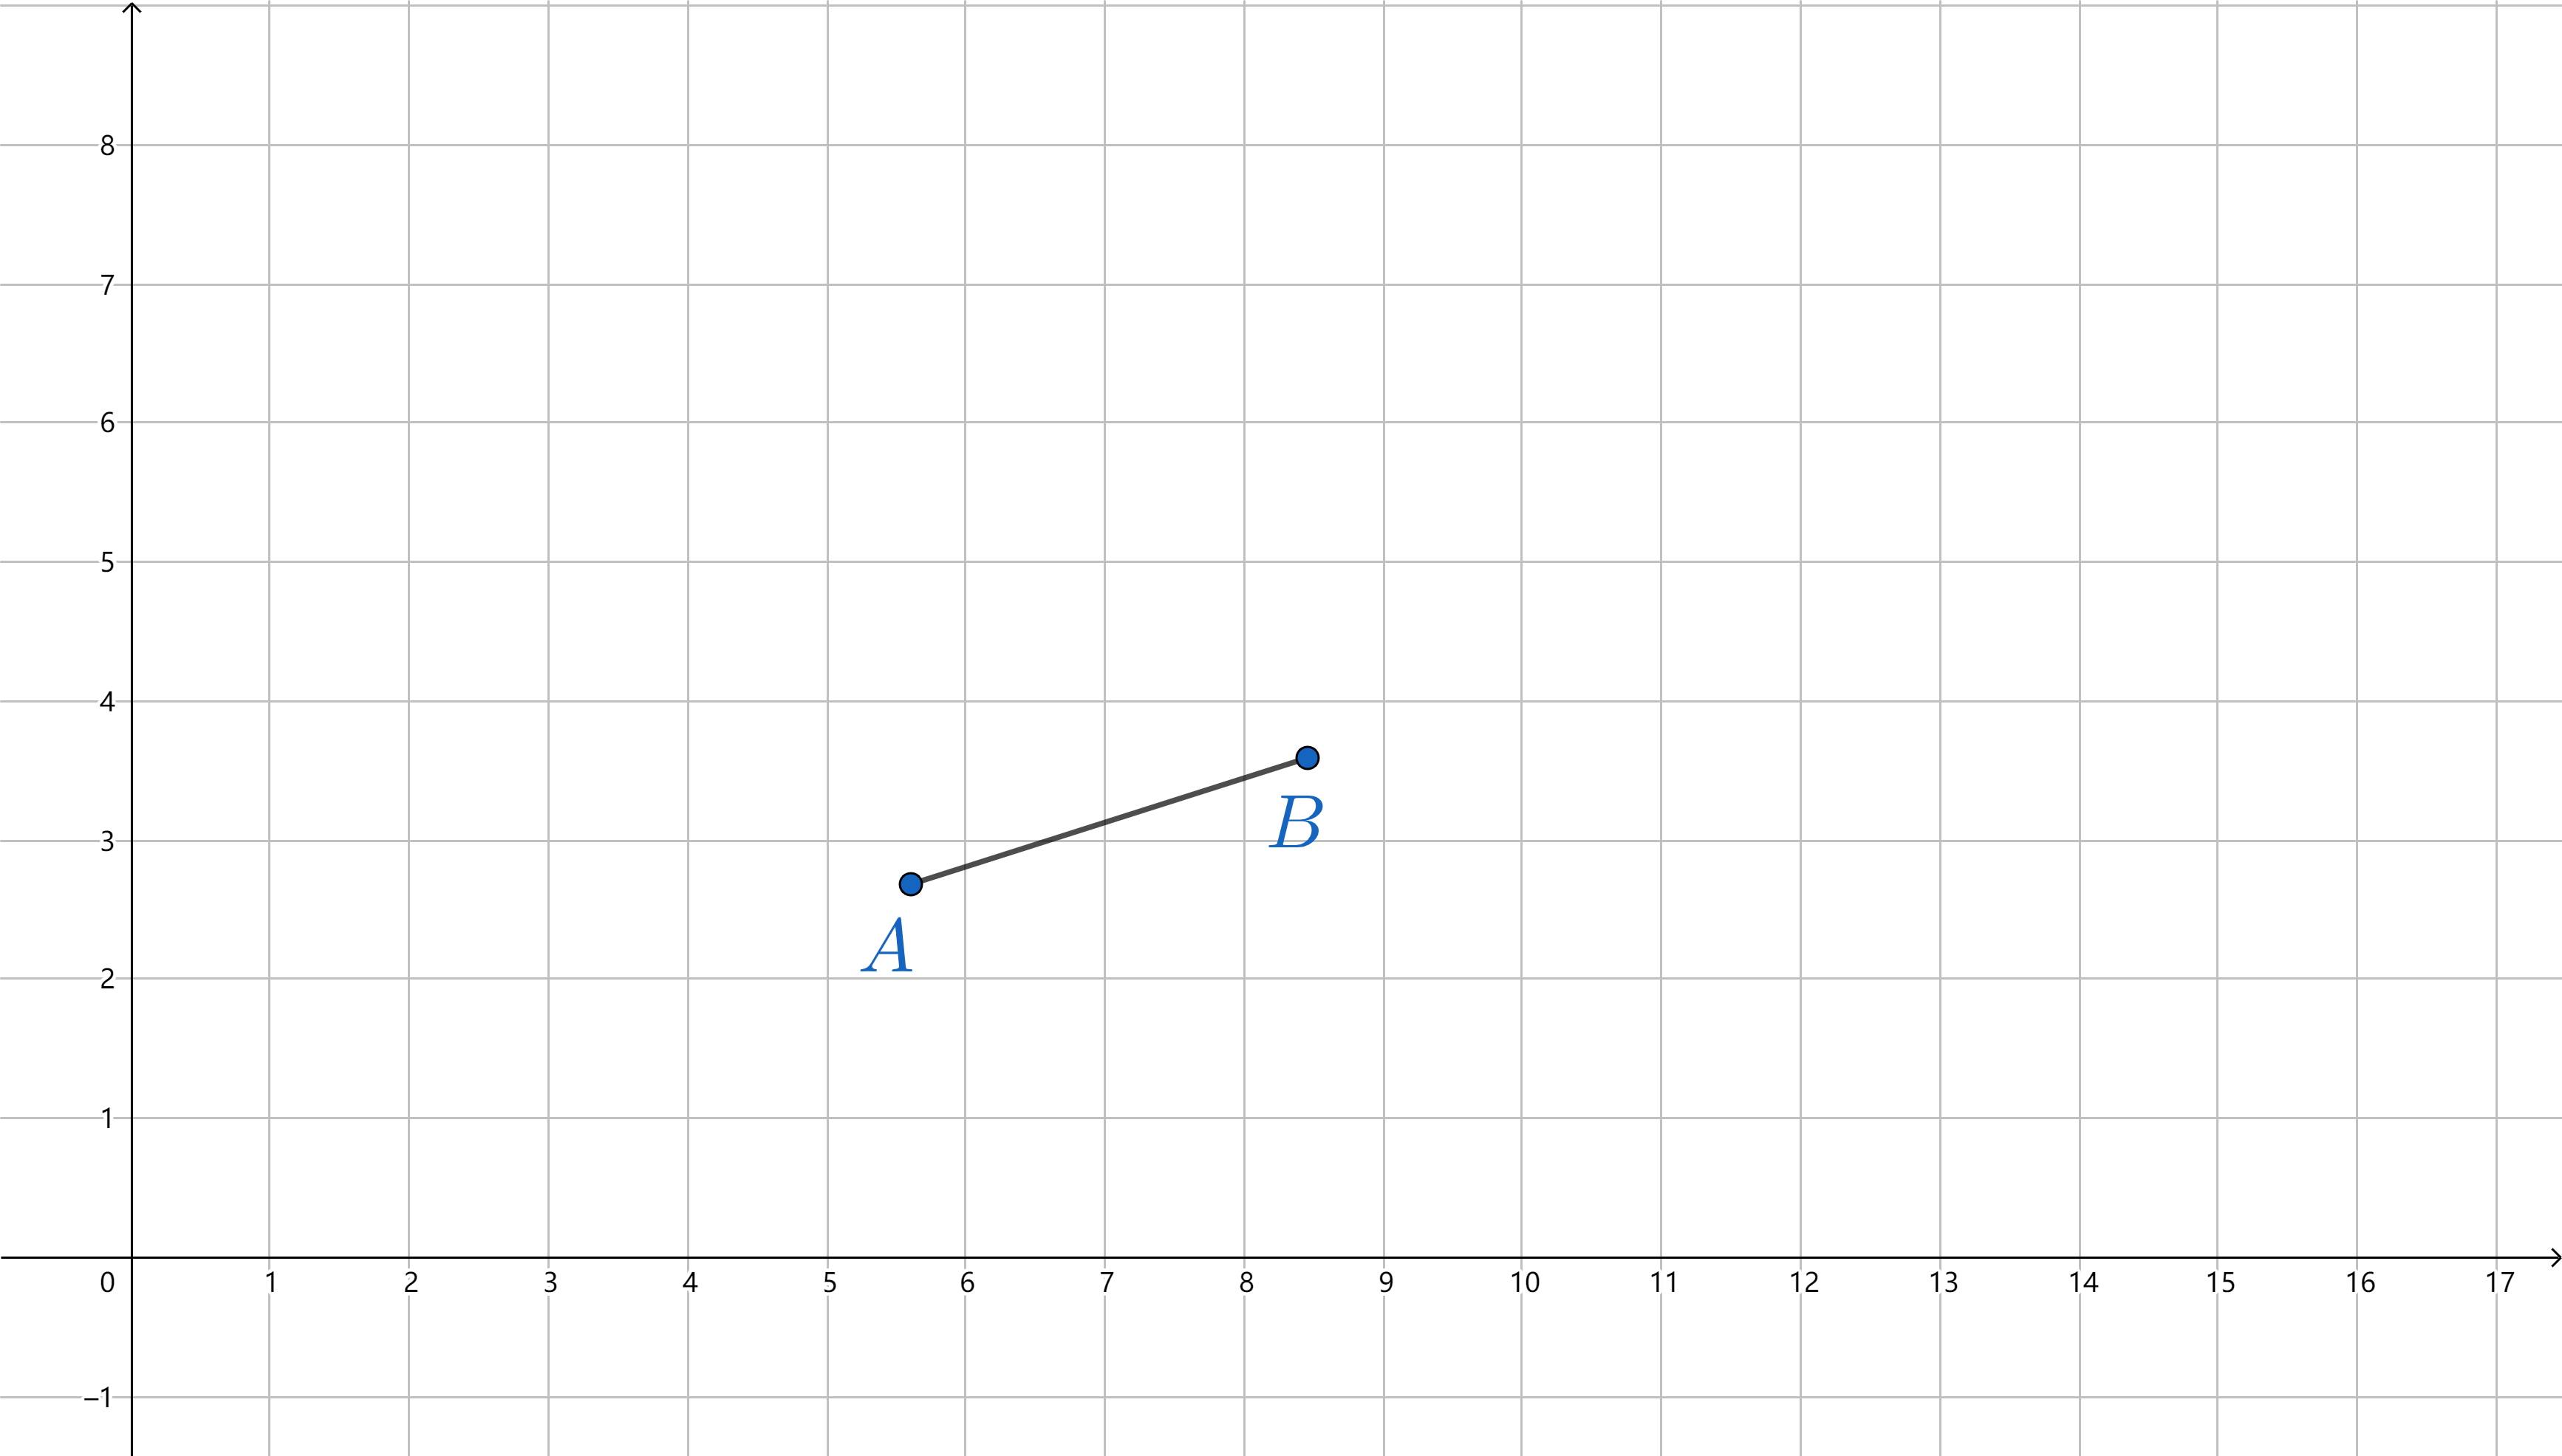
\includegraphics[width=5.76806in,height=3.27847in]{media/image23.png}

如图,\(AB\) 是任意线段,平分 \(AB\)。

我们可以利用构造重心的方法来解决这个问题。

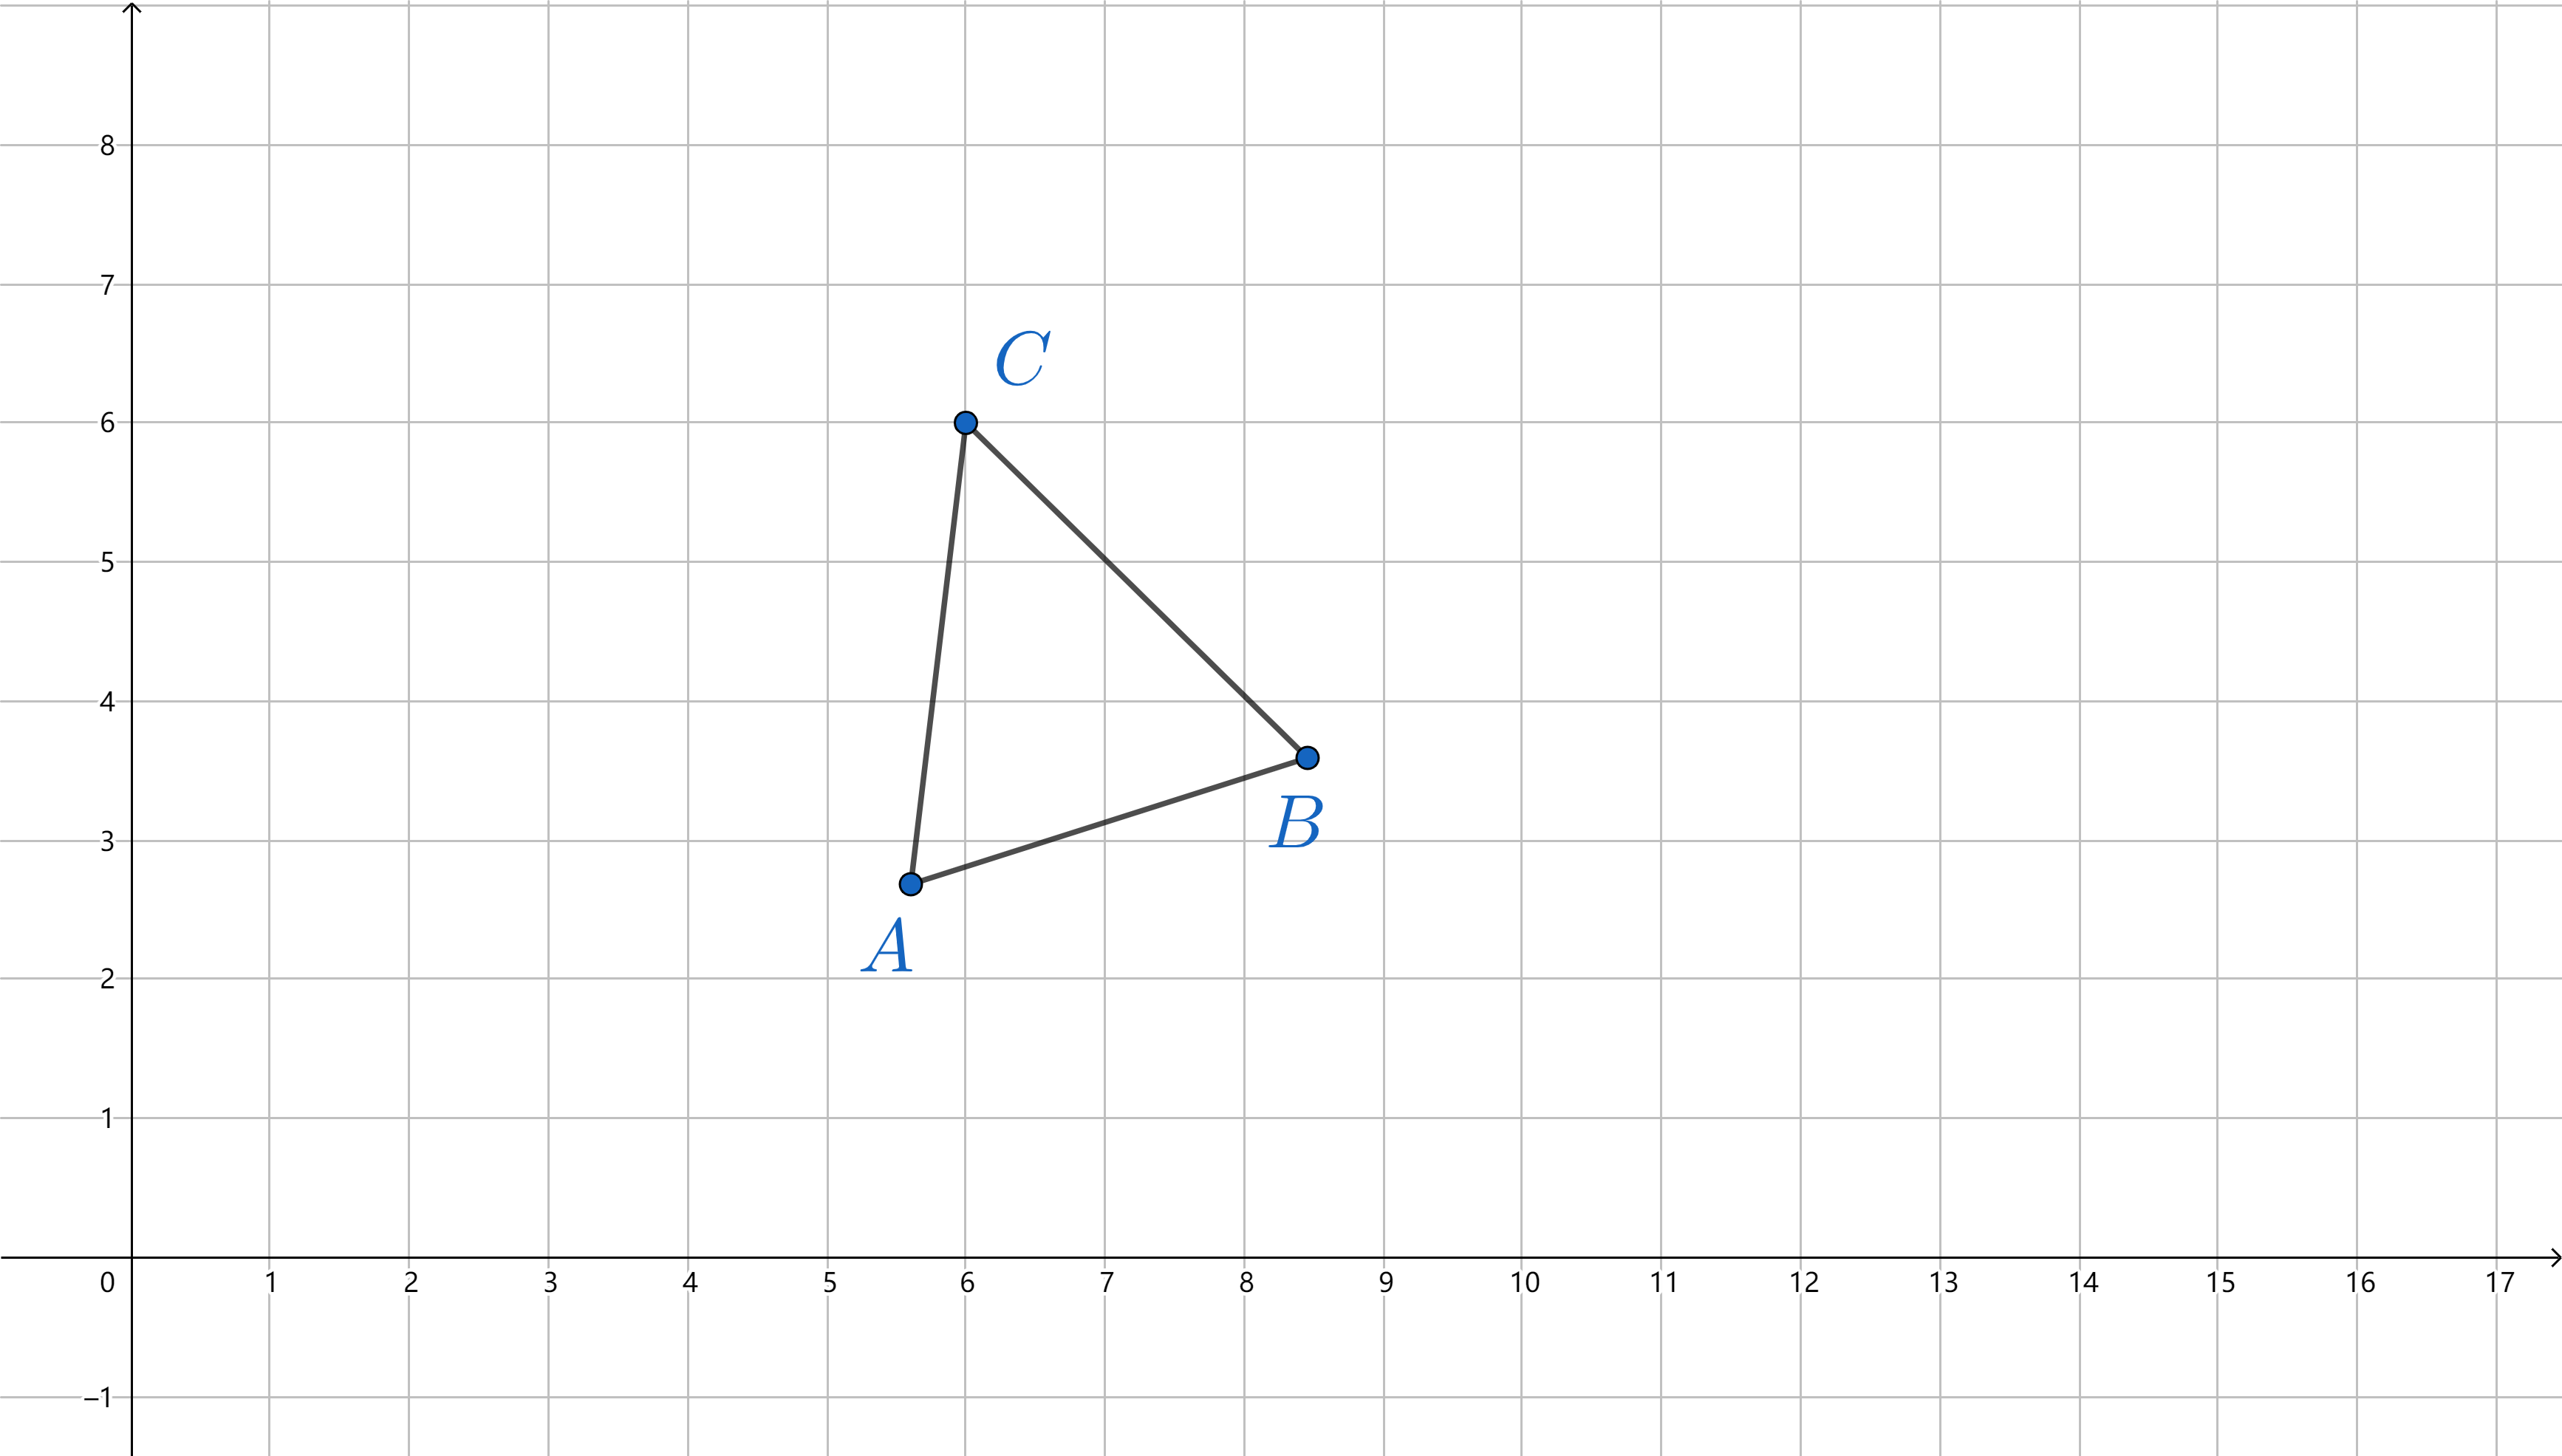
\includegraphics[width=5.76806in,height=3.27847in]{media/image24.png}

如图,\(C\) 是格点。如果我们可以作出线段 \(AC\),线段 \(BC\)
的中点,根据三角形三条中线交于同一点,我们可以作出线段 \(AB\)
的中点。至于前两个中点,根据Wyc分线段定理(定理3.4),是显然可作的。

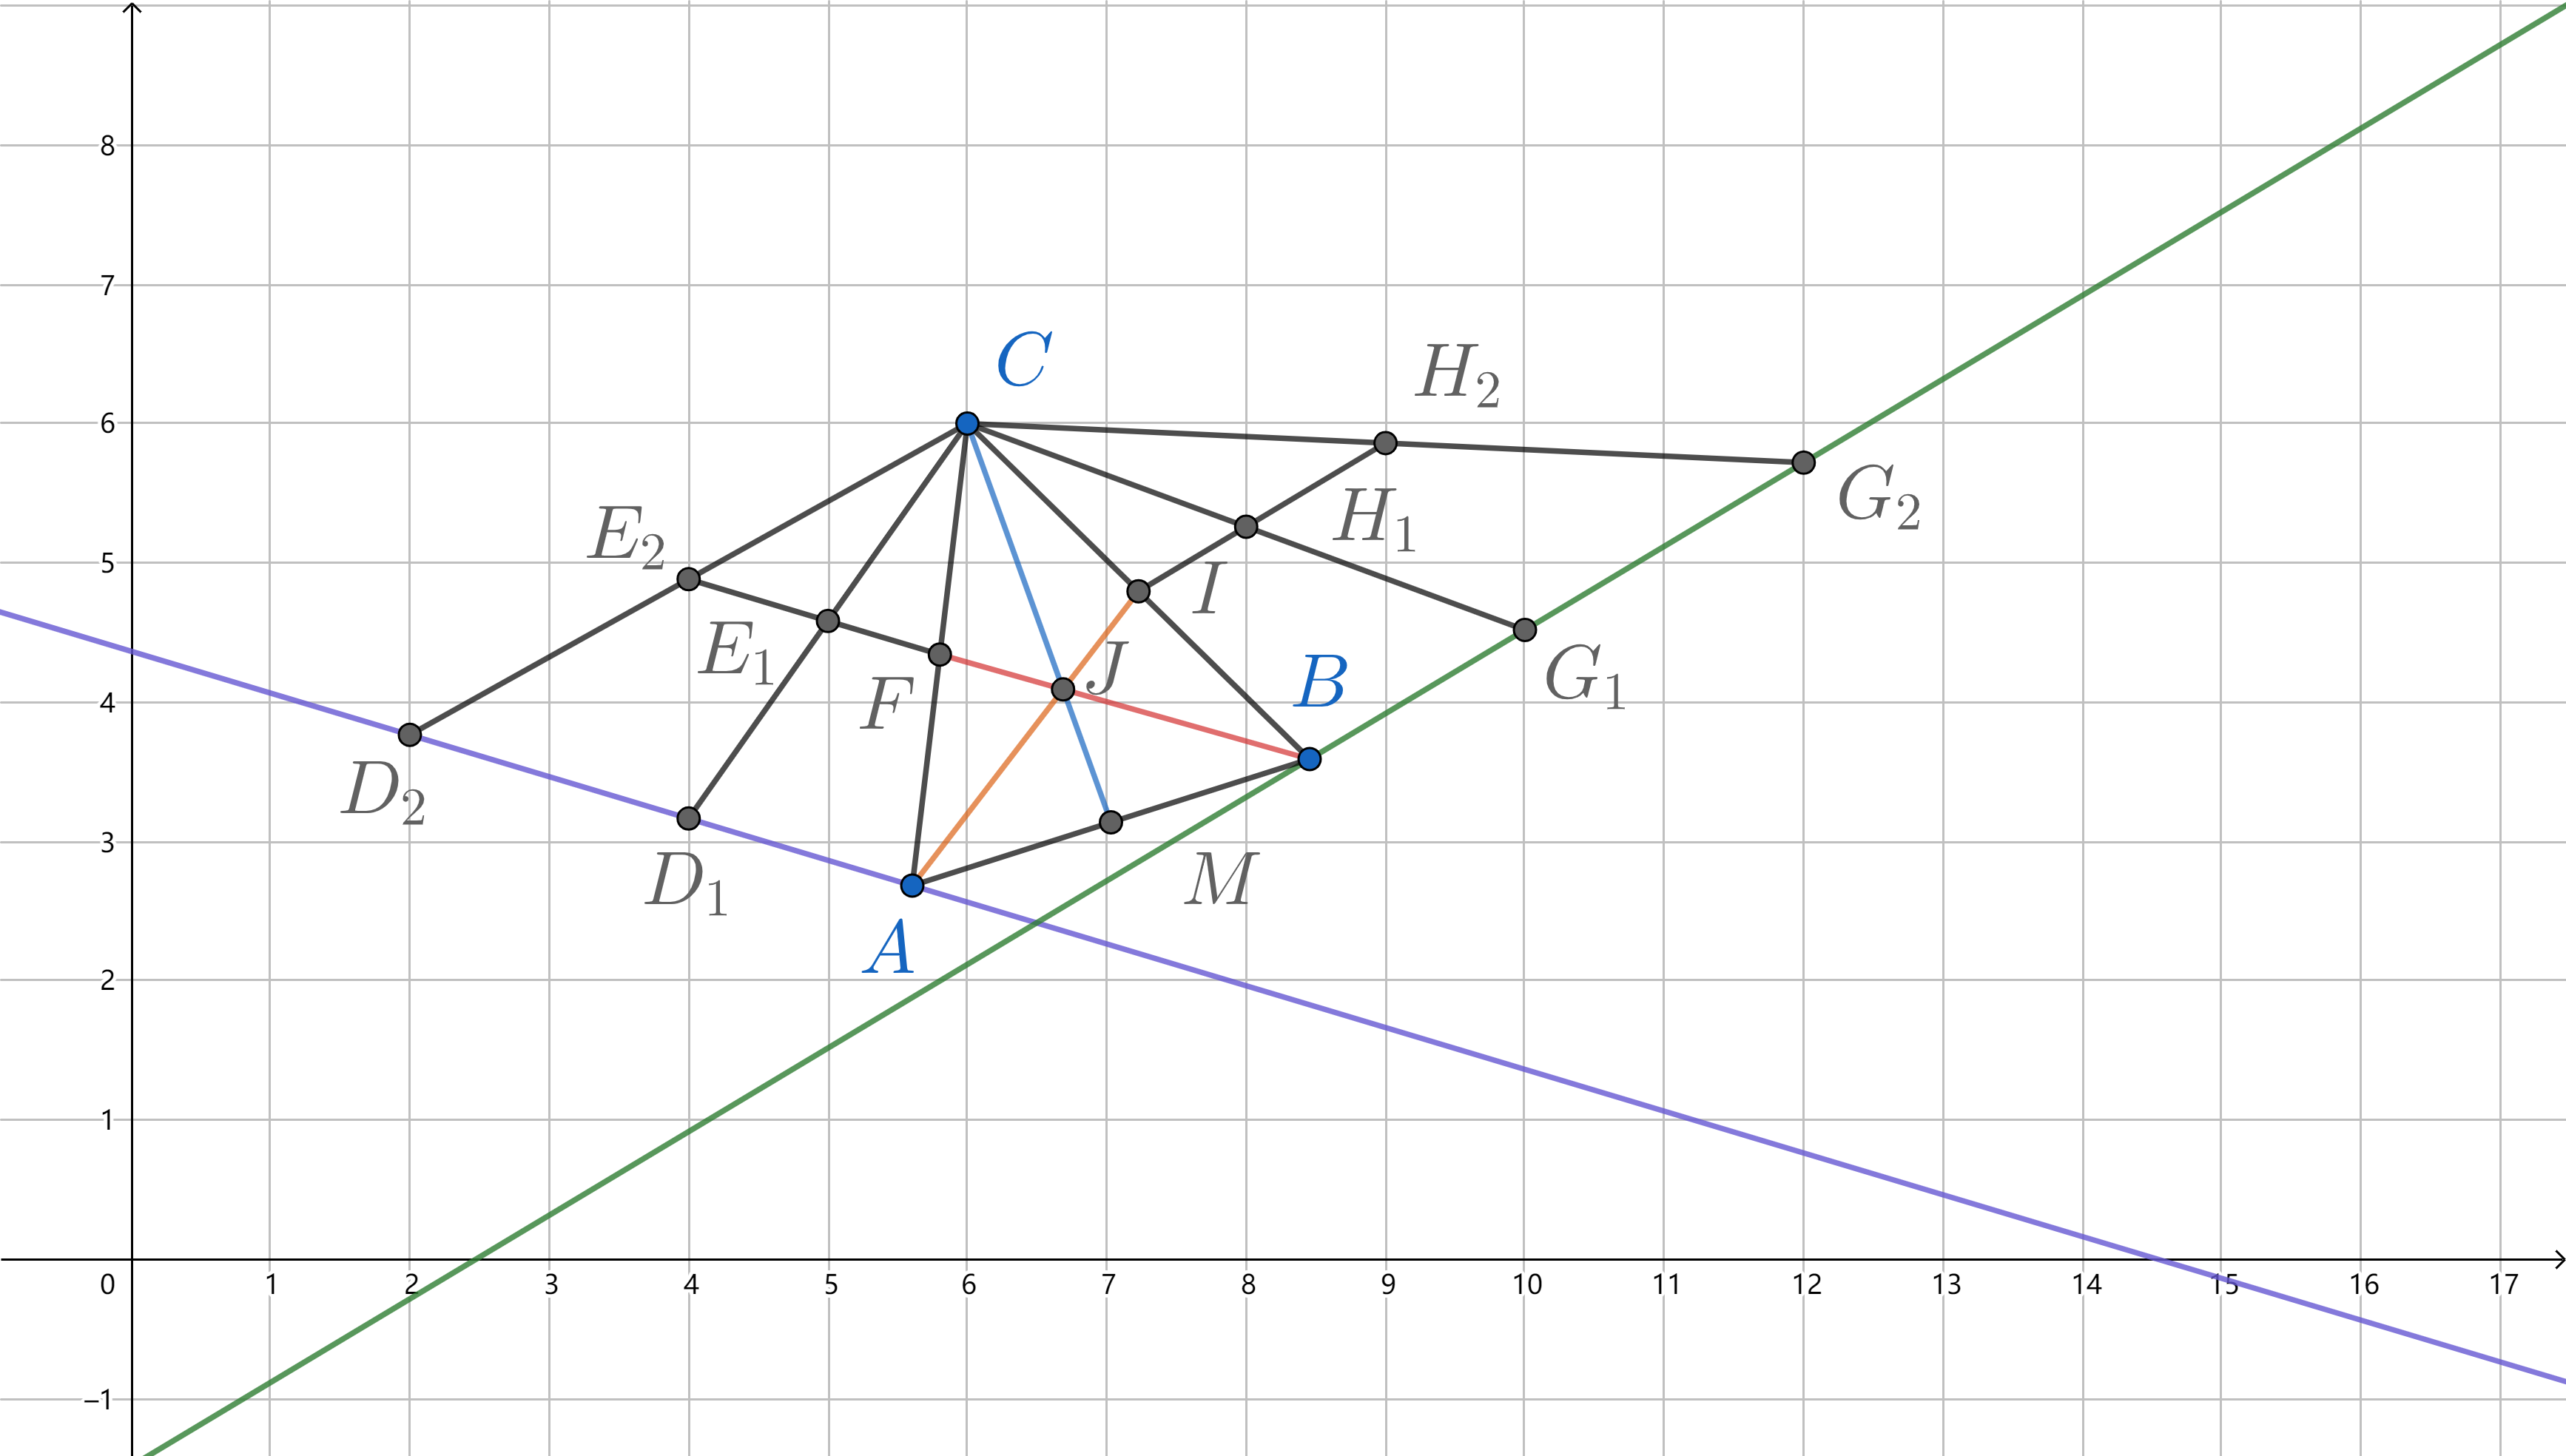
\includegraphics[width=5.76806in,height=3.27292in]{media/image25.png}

如图,用Wyc分线段定理做出线段 \(AC\) 的中点 \(F\) 和线段 \(BC\) 的中点
\(I\),连接 \(BF\) 和 \(AI\) 交于 \(J\),连接 \(CJ\) 并延长交 \(AB\) 于
\(M\),\(M\) 即为 \(AB\) 中点。读者需要注意,\(E_{2}\)、\(F\)、\(B\)
这三个点在图里看起来像是共线的三个点,实际上它们很可能不是共线的。

如果我们想要画出 \(AB\)
的三等分点、四等分点,应该怎么办呢?我们应该把这一定理扩展。通过塞瓦定理,我们可以画出三等分点,思路见下:

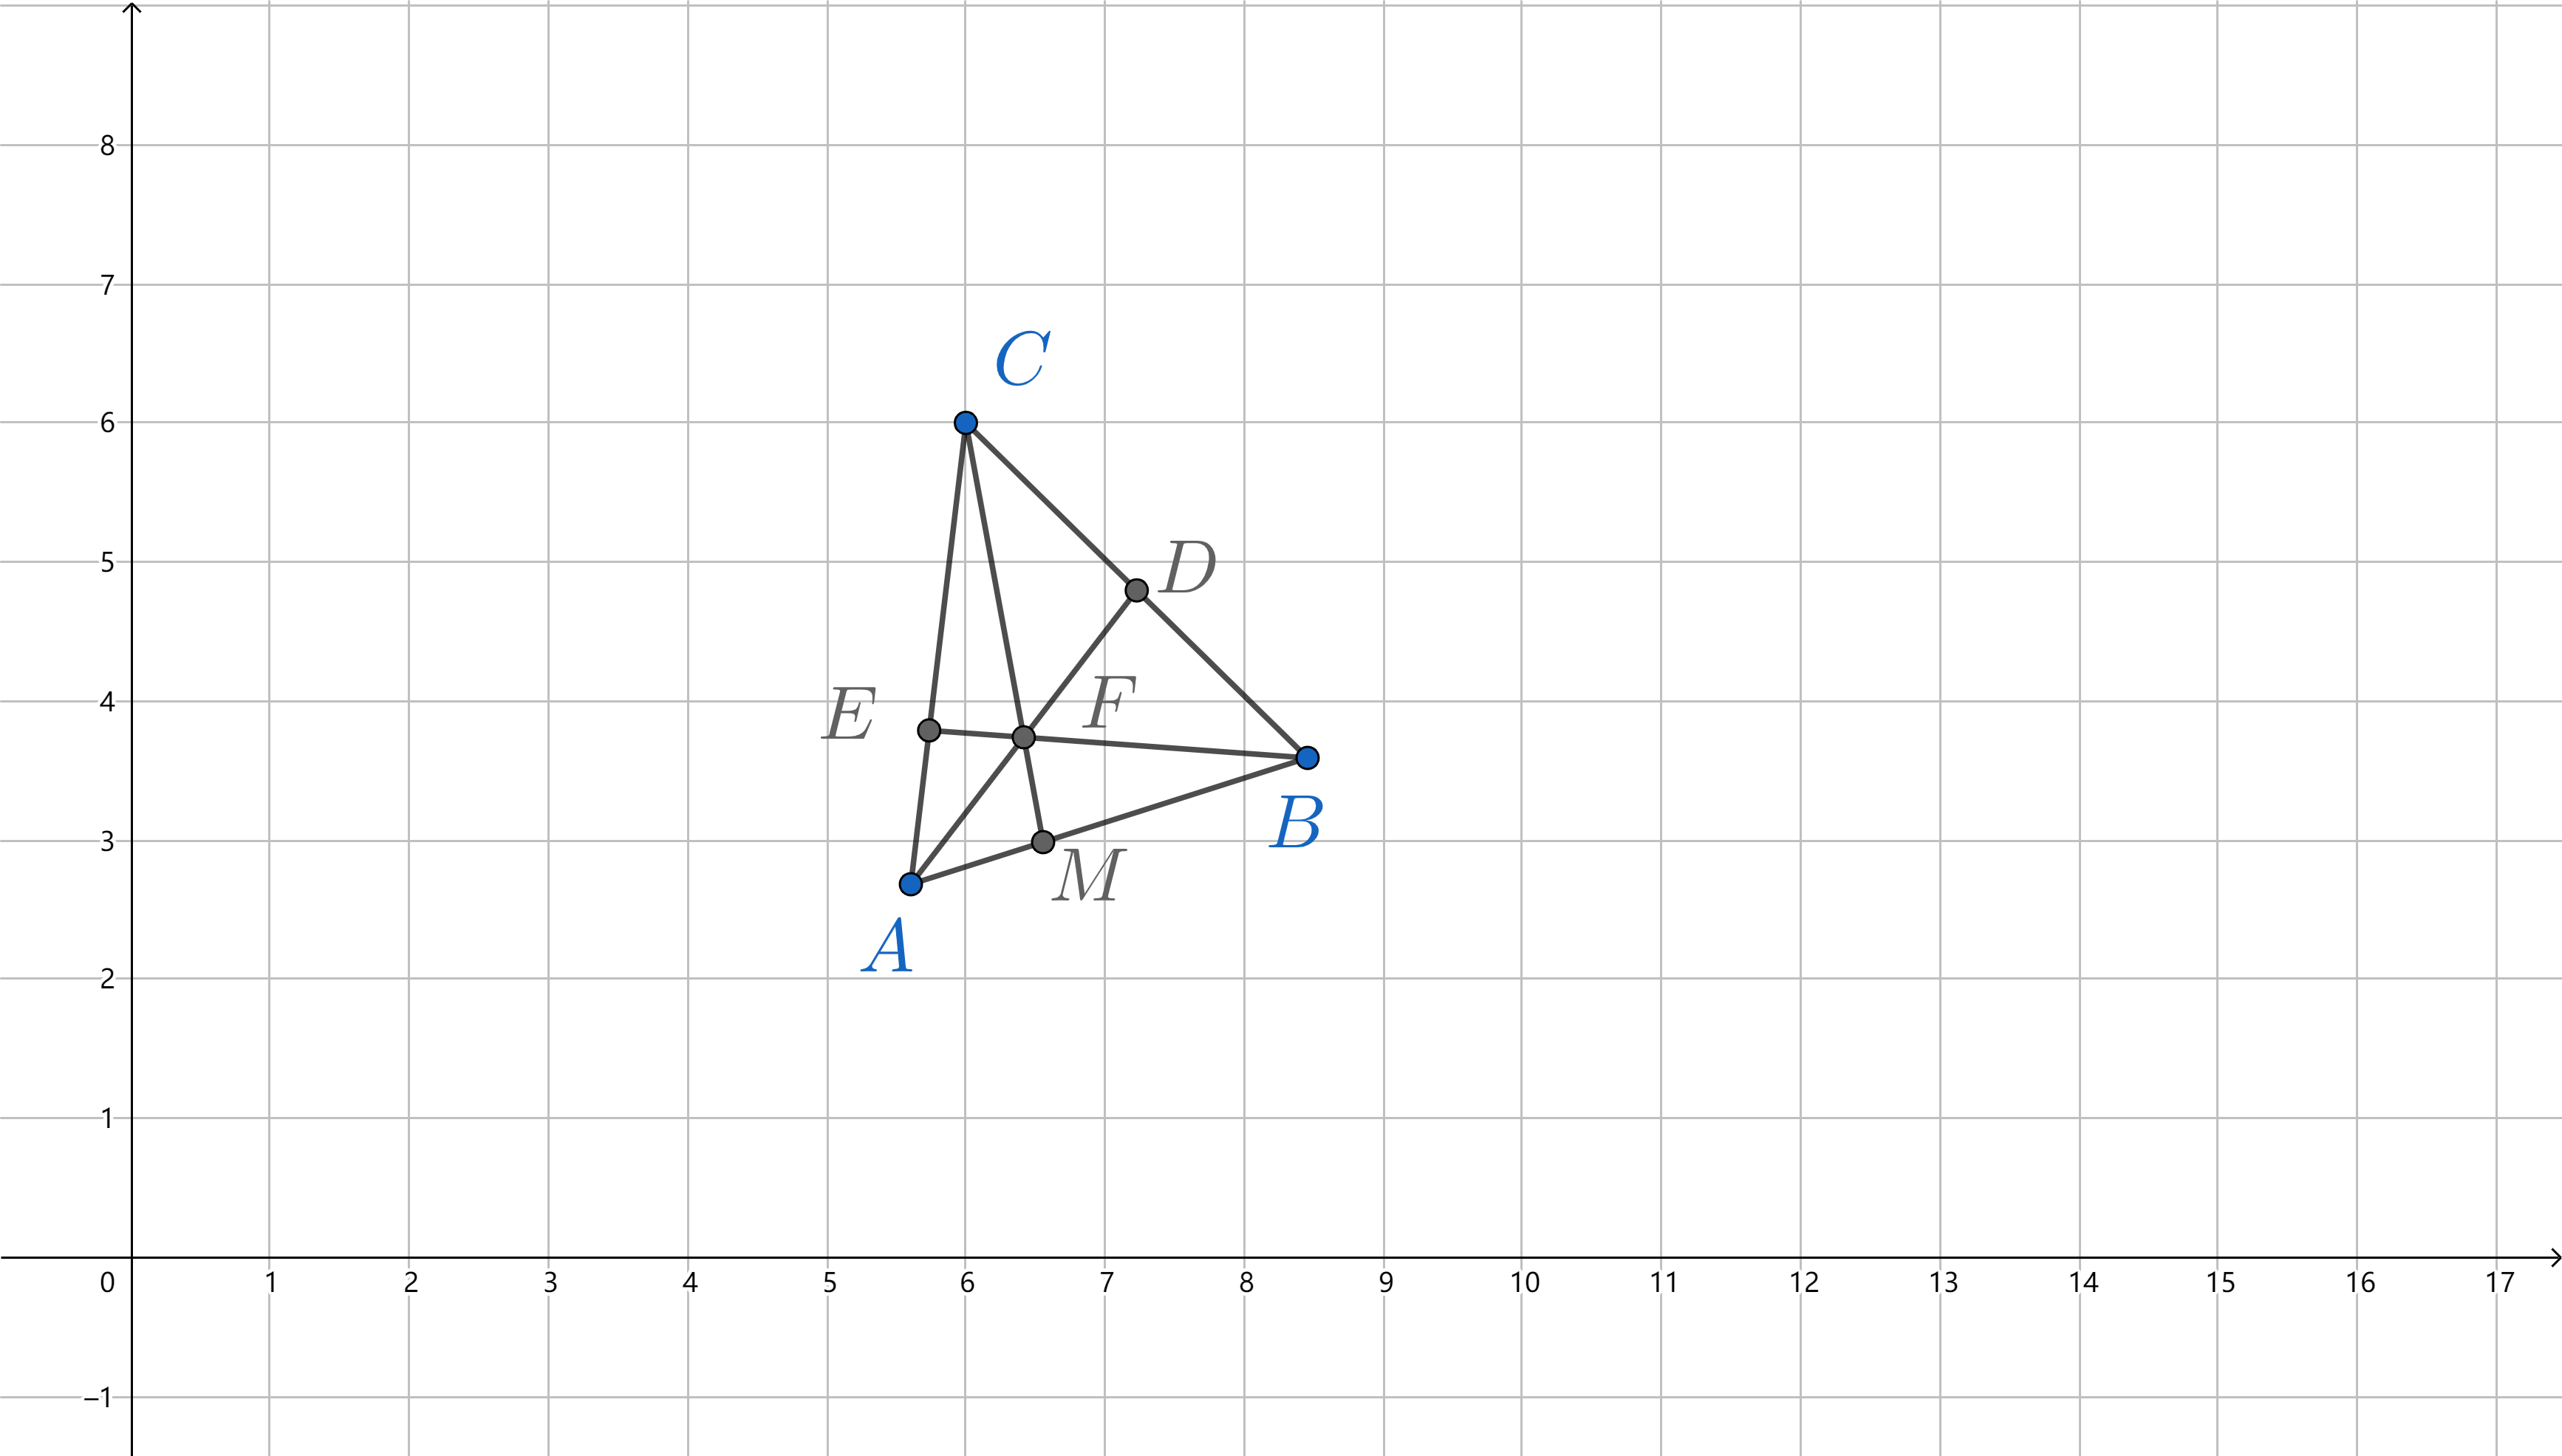
\includegraphics[width=5.76806in,height=3.27847in]{media/image26.png}

如图,\(C\) 是格点,画出线段 \(AC\) 的三等分点(更加靠近 \(A\))和
\(BC\) 的中点,连接 \(BE\)、\(AD\) 交于 \(F\),连接 \(CF\) 并延长交
\(AB\) 于 \(M\),\(M\) 即为 \(AB\) 三等分点(更靠近 \(A\) 的那一个)。

这个做法涉及到了三角形内三线共点的情况,这让我们想到了塞瓦定理:

\[\frac{CE}{AE} \cdot \frac{AM}{BM} \cdot \frac{BD}{DC} = 1\]

因为

\[\frac{CE}{AE} = 2\]

\[\frac{CD}{BD} = 1\]

所以

\[\frac{AM}{BM} = \frac{1}{2}\]

结论得证。\(M\) 的确是线段 \(AB\) 更靠近 \(A\)
的那一个三等分点。对于四等分点和其它的情况,读者可自行思考。

\hypertarget{ux5e7fux4e49wycux5206ux7ebfux6bb5ux5b9aux7406wycs-generalized-segment-dividing-theoremux5b9aux7406-3.5}{%
\subsection{广义Wyc分线段定理Wyc's Generalized Segment Dividing
Theorem(定理
3.5)}\label{ux5e7fux4e49wycux5206ux7ebfux6bb5ux5b9aux7406wycs-generalized-segment-dividing-theoremux5b9aux7406-3.5}}

\textbf{【提出者】}翟悦凯(广义定理非王宇辰本人提出)

对于任意一条线段,可以用比平分线段定理(定理
3.1.2)更简单的方法,把该线段分成给定比例。

\textbf{【优化】}当我们想要做出一条任意线段的中点时,做法可以进一步优化。我们先来看图。

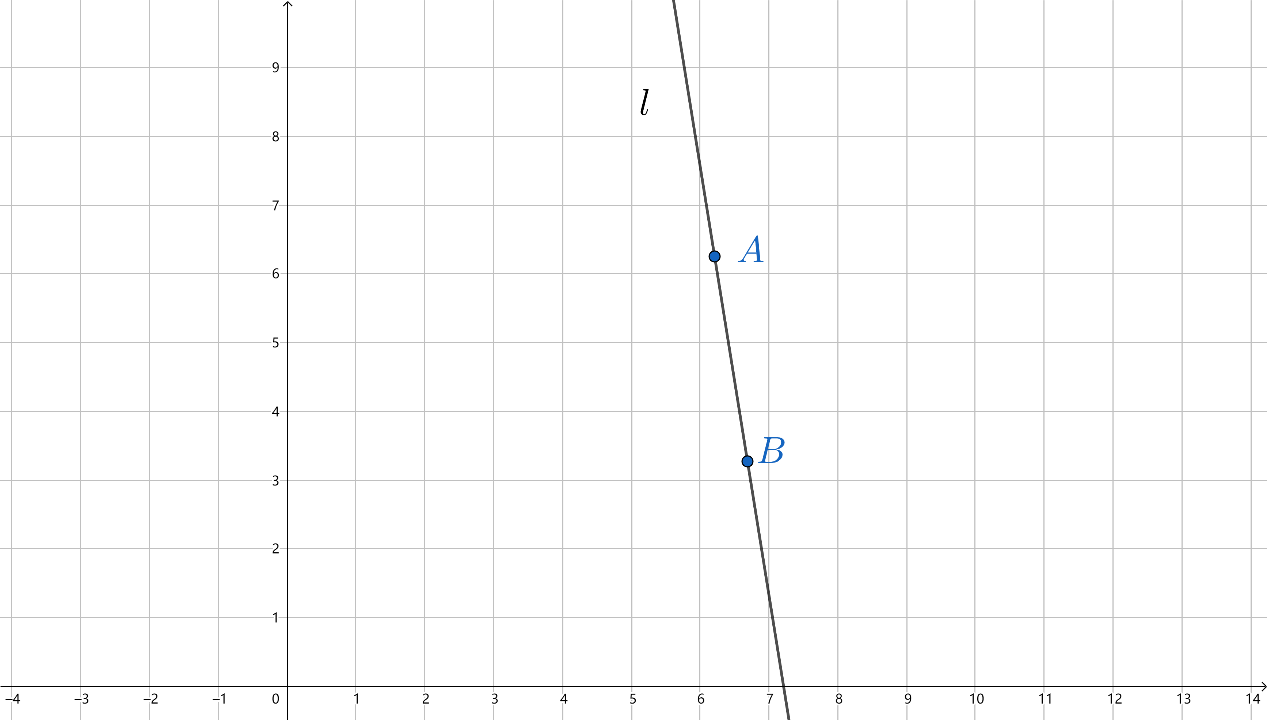
\includegraphics[width=5.75833in,height=3.275in]{media/image27.png}

如图,在线段 \(AB\) 上找到它的中点。

首先我们要做 \(AB\)
的平行线。为了方便,我们可以充分利用格线,不用张世其平行定理来画平行线。

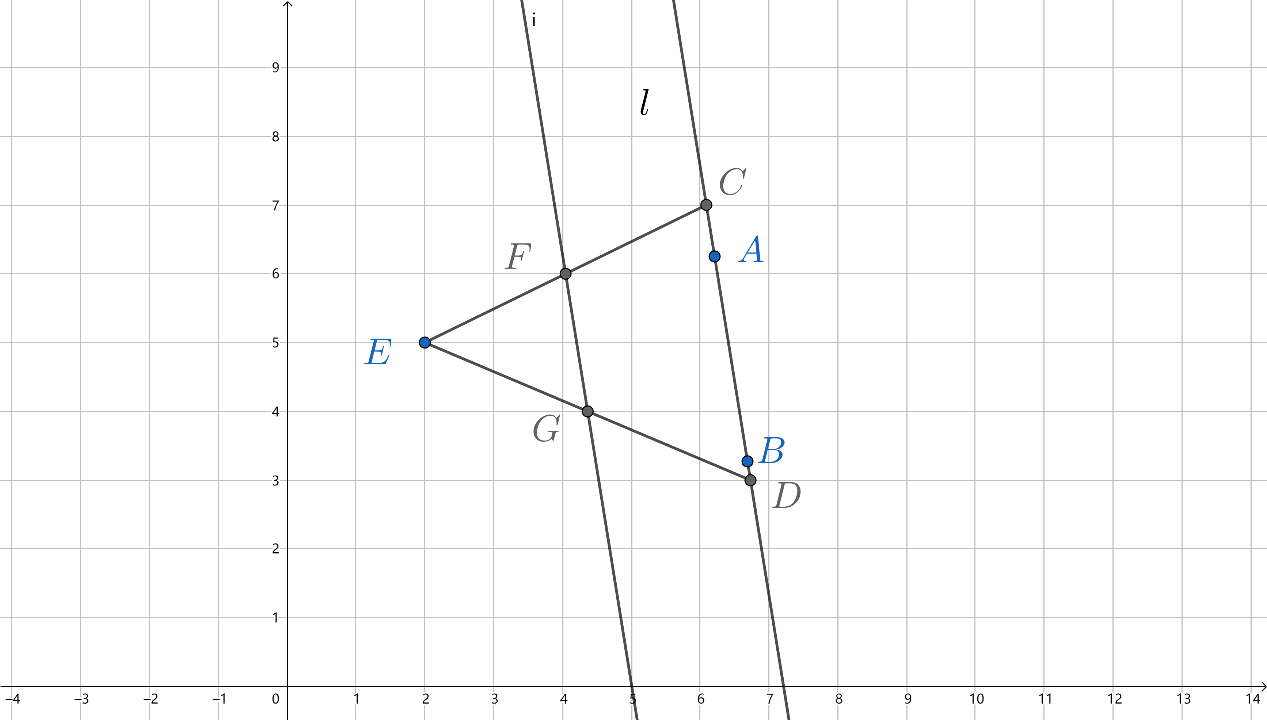
\includegraphics[width=5.75833in,height=3.275in]{media/image28.png}

如图,取格点 \(C\),\(D\),\(E\),连 \(EC\) 交格线于 \(F\),连 \(ED\)
交格线于 \(G\),连接 \(FG\),那么 \(FG \parallel CD\)。

因为 \(FG \parallel CD\),所以在 \(CD\) 上的任意一点 \(P\),连接 \(EP\)
交 \(FG\) 于 \(Q\),都满足
\(EP = 2EQ\)。我们可以利用这一特性来构造重心。

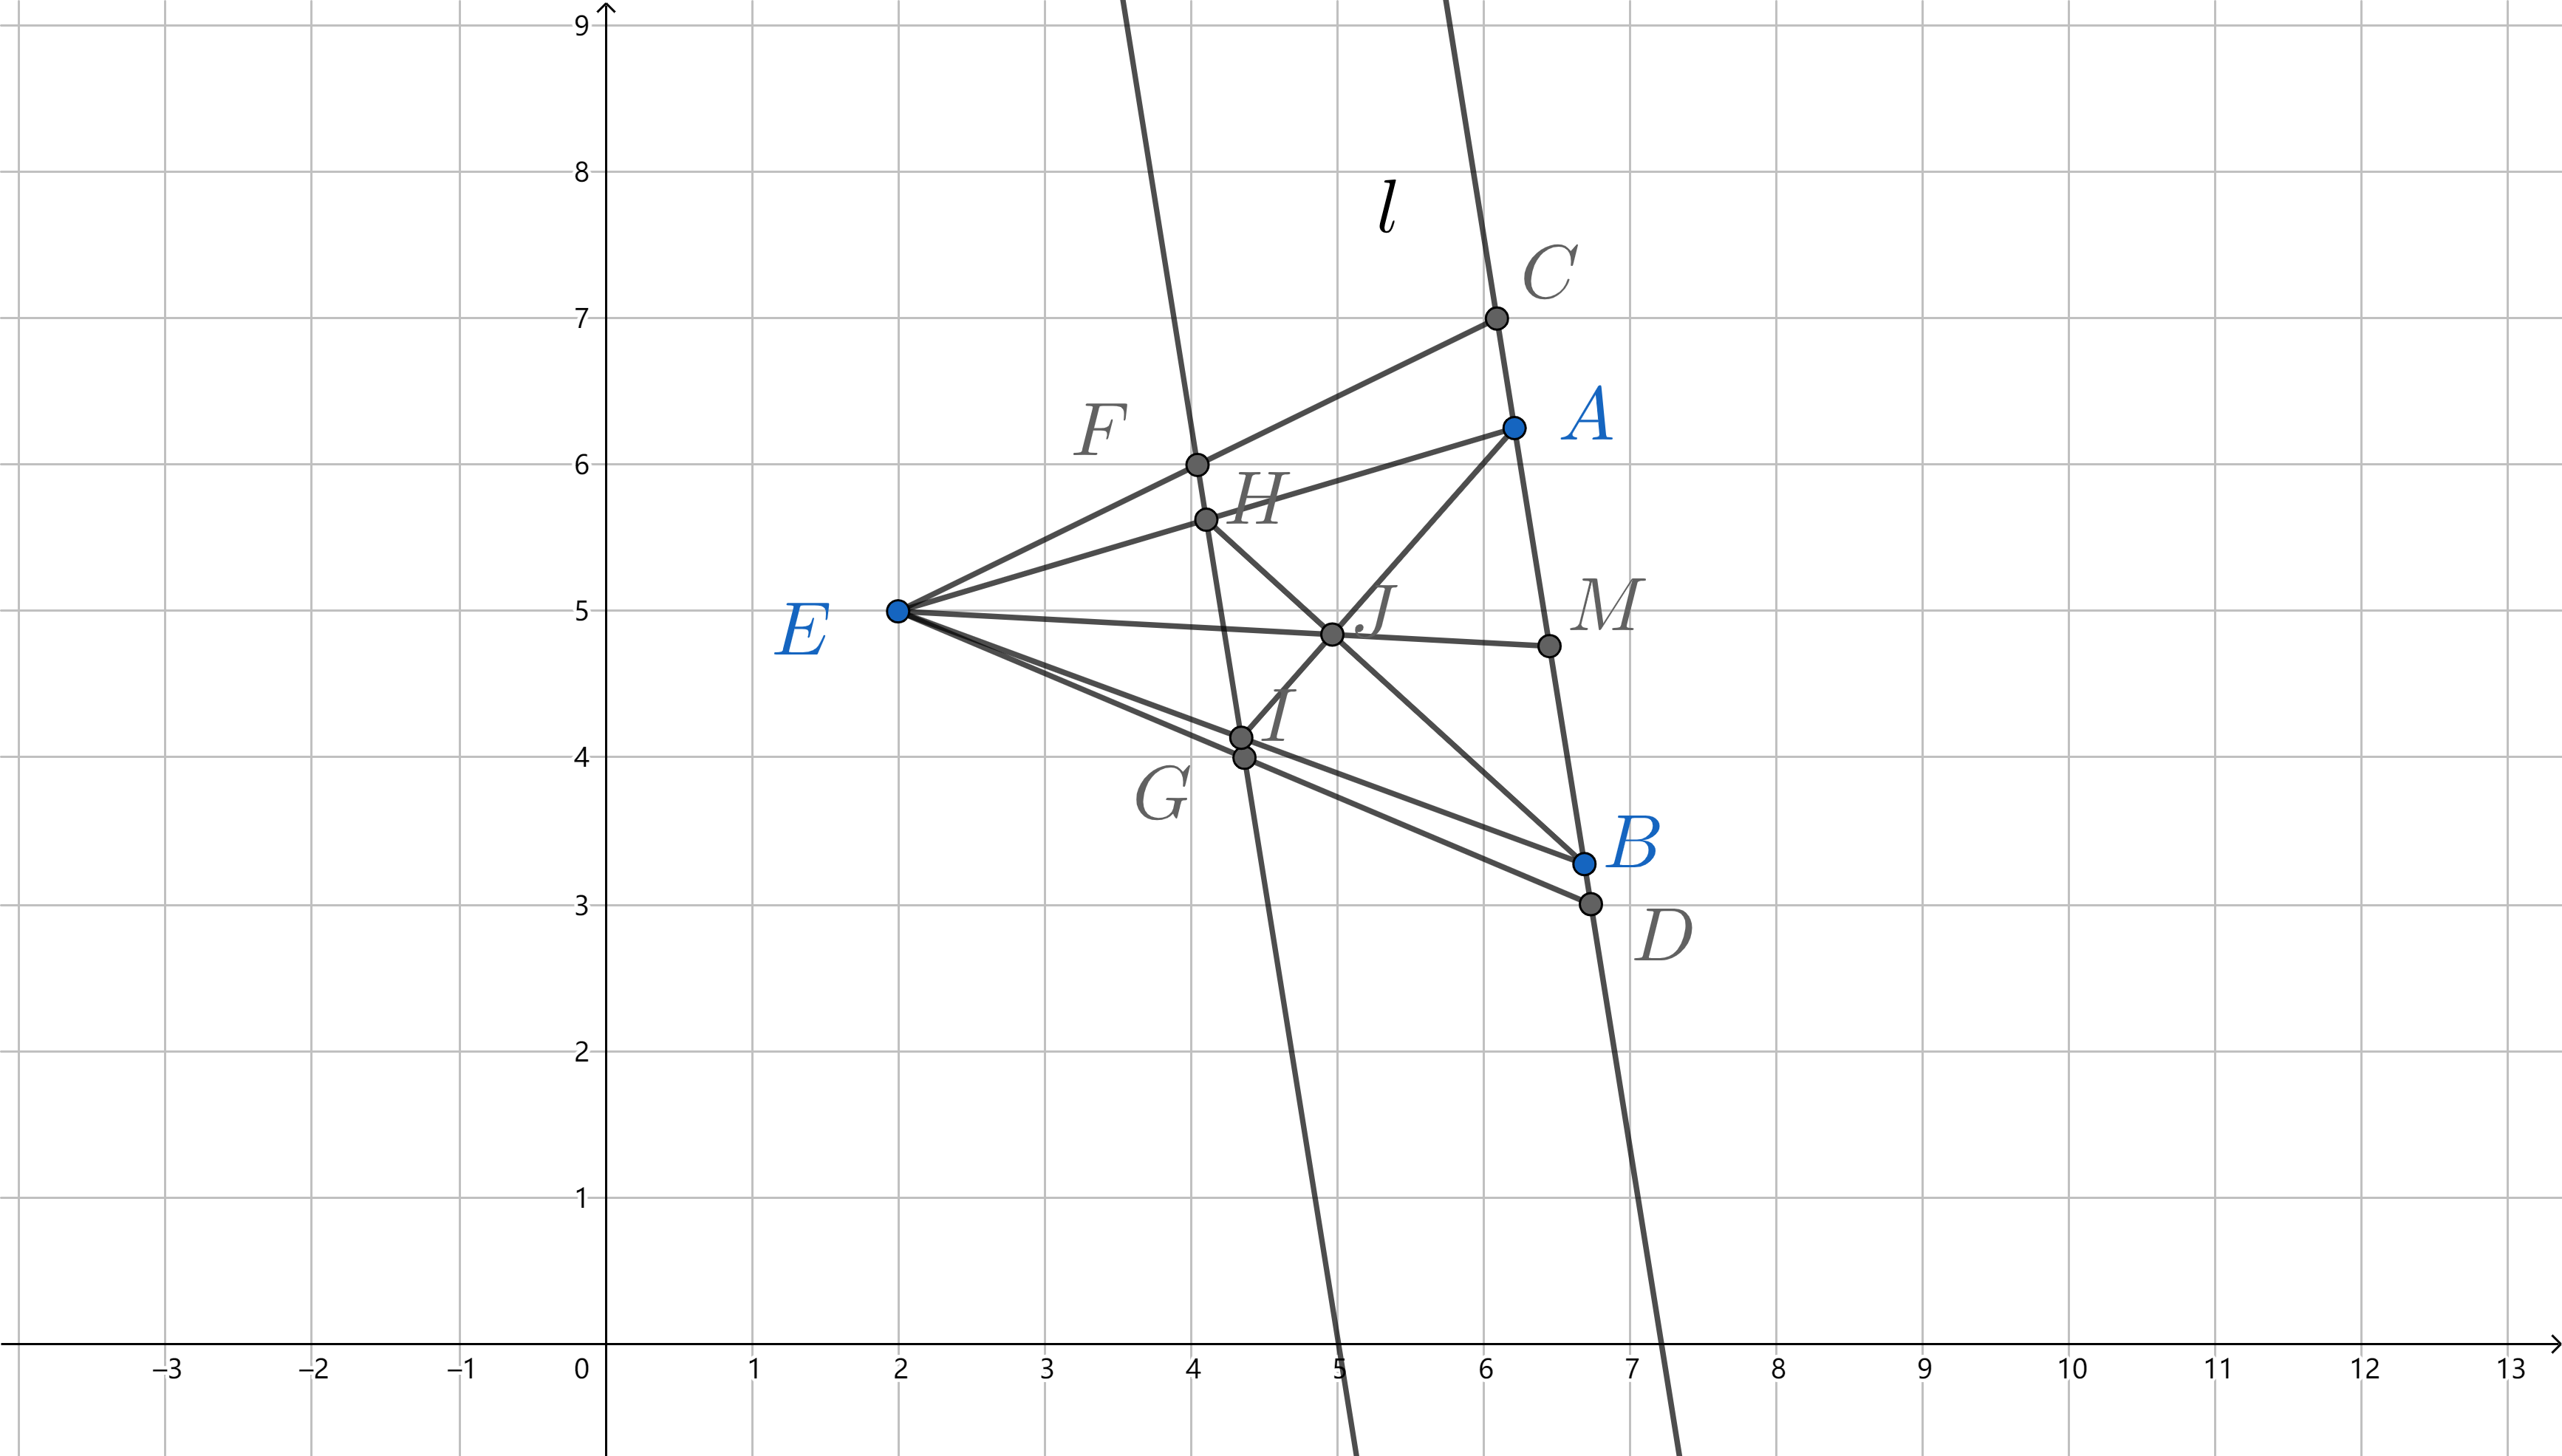
\includegraphics[width=5.76806in,height=3.27847in]{media/image29.png}

如图,连接 \(EA\),\(EB\) 交 \(FG\) 分别于 \(H\),\(I\)。连接
\(BH\),\(AI\) 交于 \(J\)。连接 \(EJ\) 并延长交 \(AB\) 于 \(M\)。\(M\)
即为 \(AB\) 的中点。这个优化由欧思远给出。

\hypertarget{ux5e7fux4e49wycux5206ux7ebfux6bb5ux5b9aux7406ux7684osyux7b2cux4e00ux4f18ux5316-osys-first-optimization-of-wycs-generalized-segment-dividing-theoremux5b9aux7406-3.5.1}{%
\subsection{广义Wyc分线段定理的Osy第一优化 Osy's First Optimization of
Wyc's Generalized Segment Dividing Theorem(定理
3.5.1)}\label{ux5e7fux4e49wycux5206ux7ebfux6bb5ux5b9aux7406ux7684osyux7b2cux4e00ux4f18ux5316-osys-first-optimization-of-wycs-generalized-segment-dividing-theoremux5b9aux7406-3.5.1}}

【提出者】欧思远

对于任意一条线段,我们可以用比广义Wyc分线段定理(定理
3.5)更简单的方法来平分它。

\textbf{注意}:定理 3.5.1 只能平分一条线段,不能把它分成其它的比例。

\hypertarget{wycux4e24ux5927ux500dux957fux7ebfux6bb5ux5b9aux7406}{%
\subsubsection{Wyc两大倍长线段定理}\label{wycux4e24ux5927ux500dux957fux7ebfux6bb5ux5b9aux7406}}

类似于Wyc分线段定理,当线段的一个端点在格线上时,我们可以充分利用这个端点来简化作图步骤。Wyc倍长线段定理分为两部分:一是向格线端点的方向倍长线段,一是向自由端倍长线段。我们先看向格线端点的方向倍长线段。

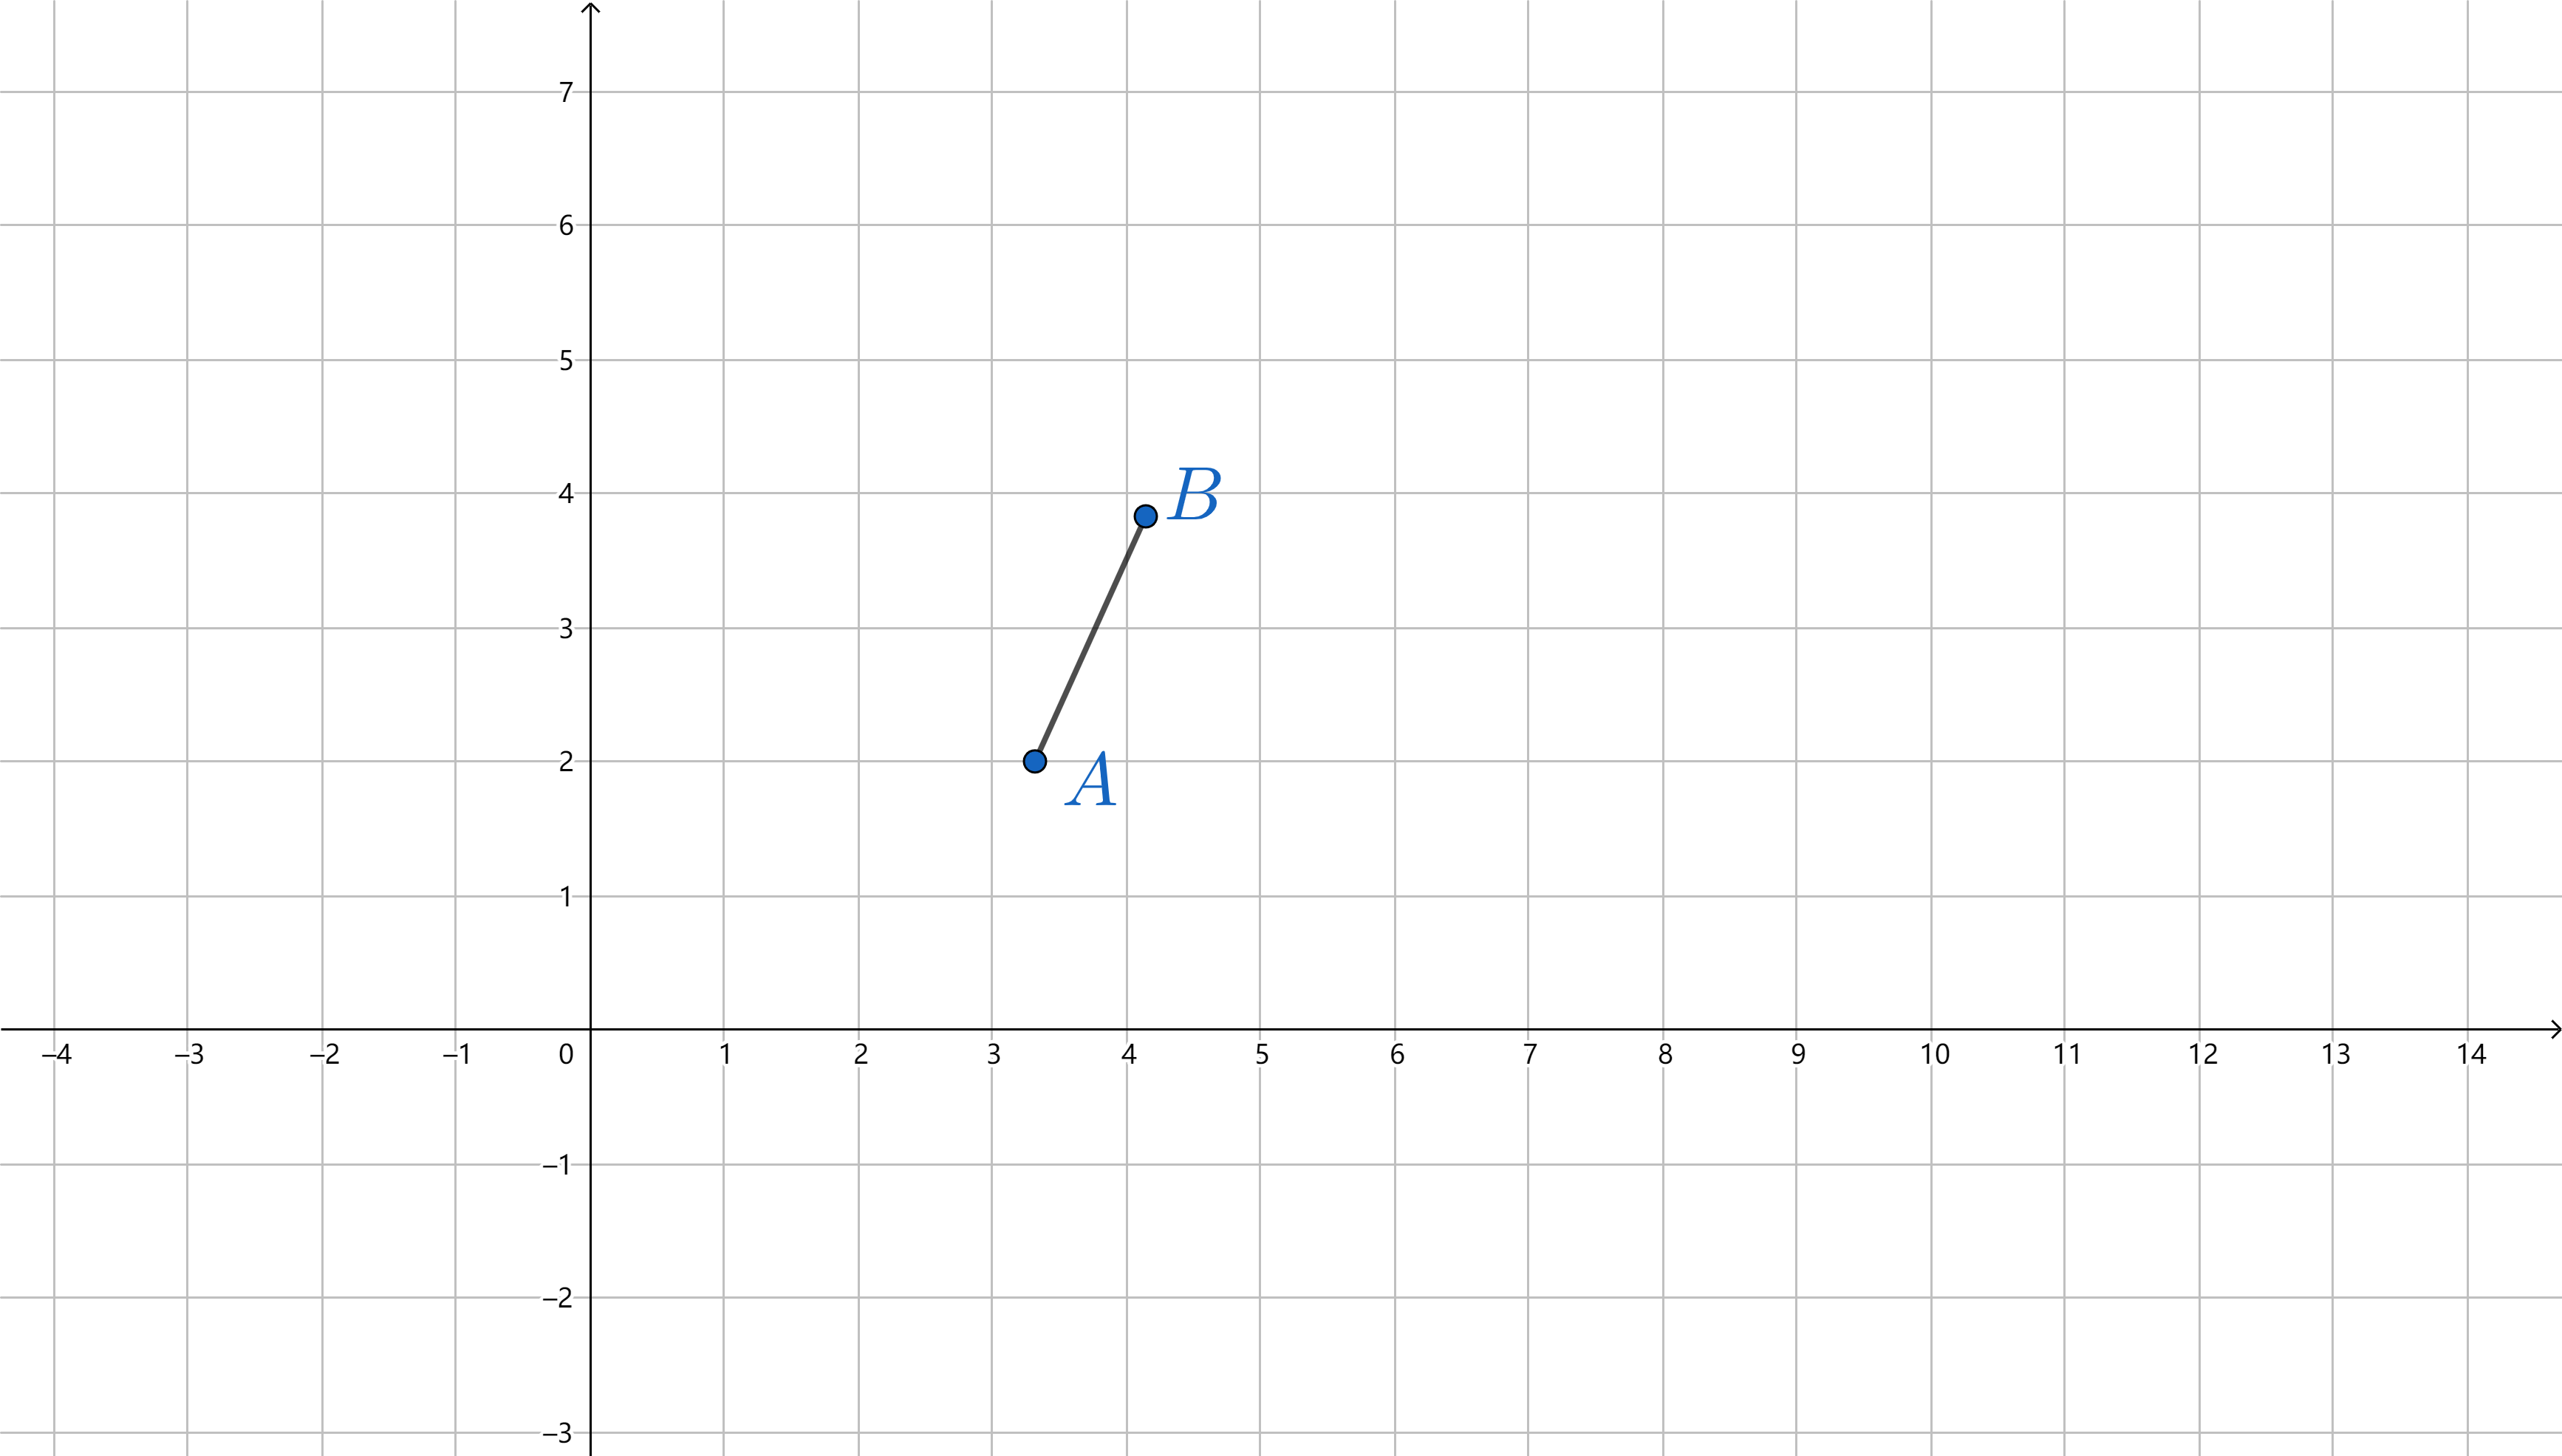
\includegraphics[width=5.76806in,height=3.27847in]{media/image30.png}

如图, \(A\) 在格线上,请延长线段 \(BA\) 到点 \(B^{'}\) 使得
\(AB = AB^{'}\)。

我们可以通过构造中心对称来解决这个问题。作图步骤和Wyc分线段定理有相似之处。

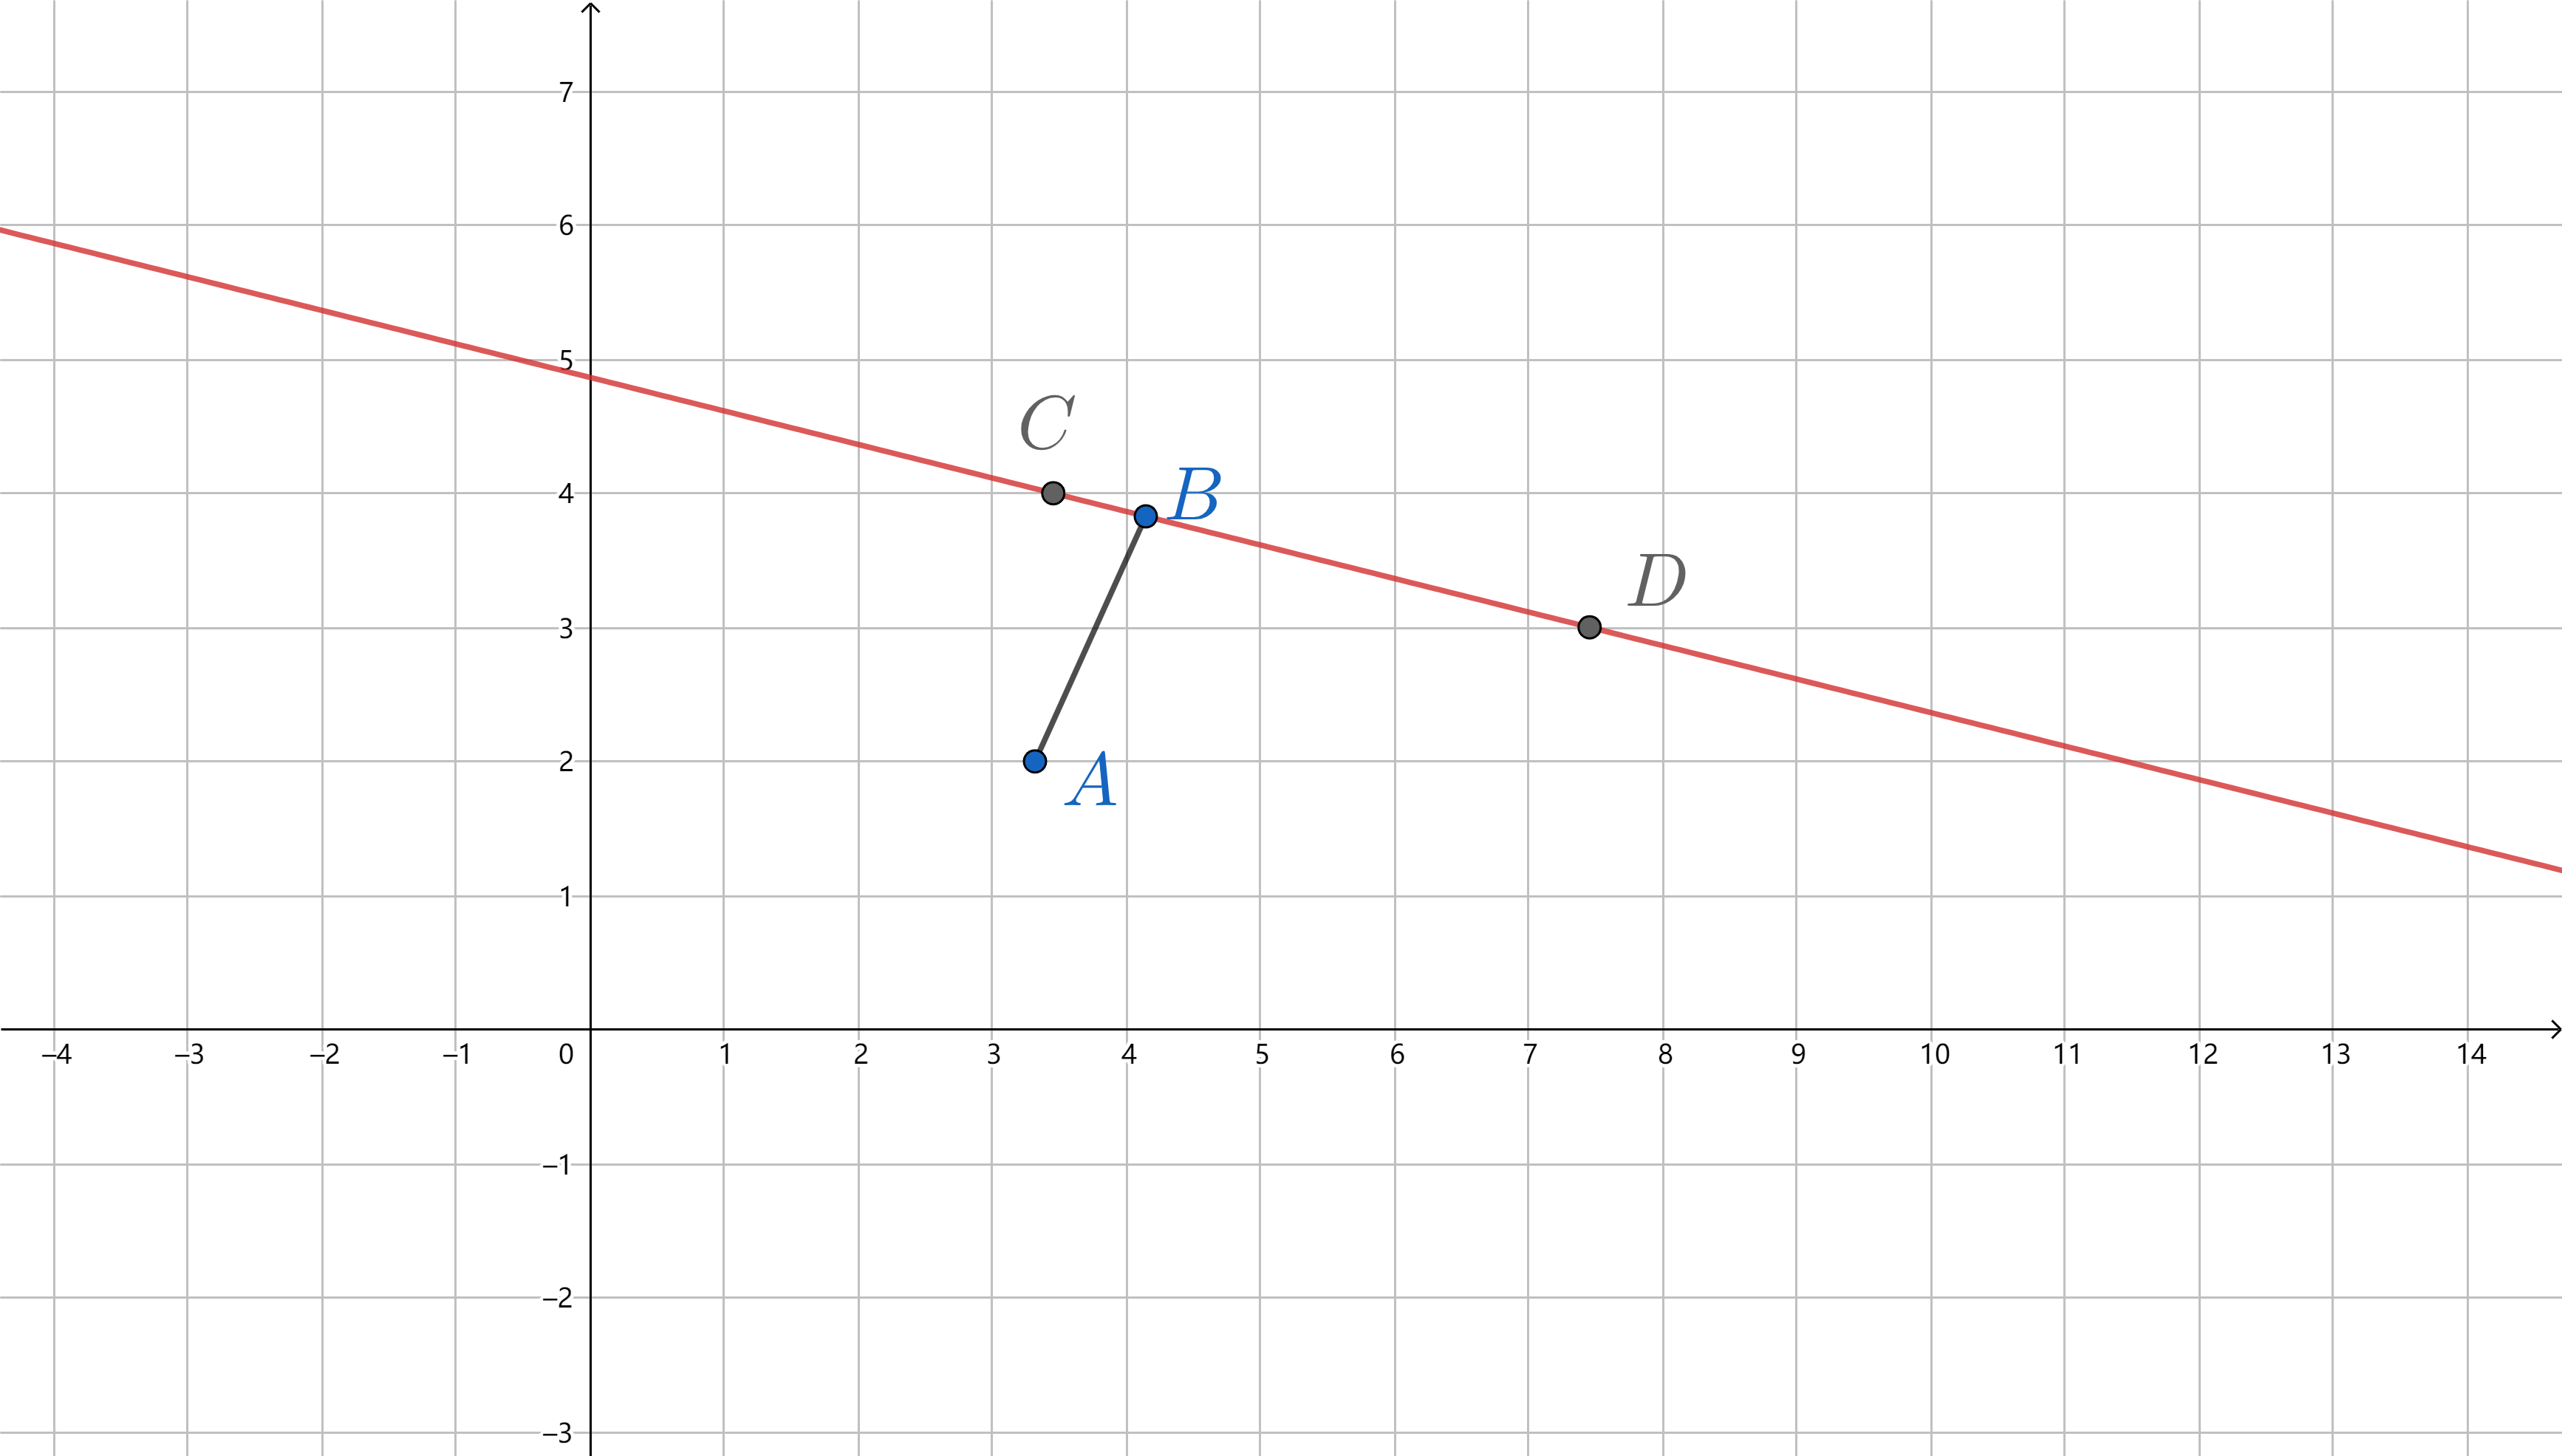
\includegraphics[width=5.76806in,height=3.27847in]{media/image31.png}

如图,过 \(B\) 作一条合适的直线,交两条水平格线分别于
\(C\),\(D\)。我们发现,利用 \(A\),\(C\),\(D\)
都在水平格线上这一个条件,可以很简单地倍长线段 \(AC\) 和线段 \(AD\)。

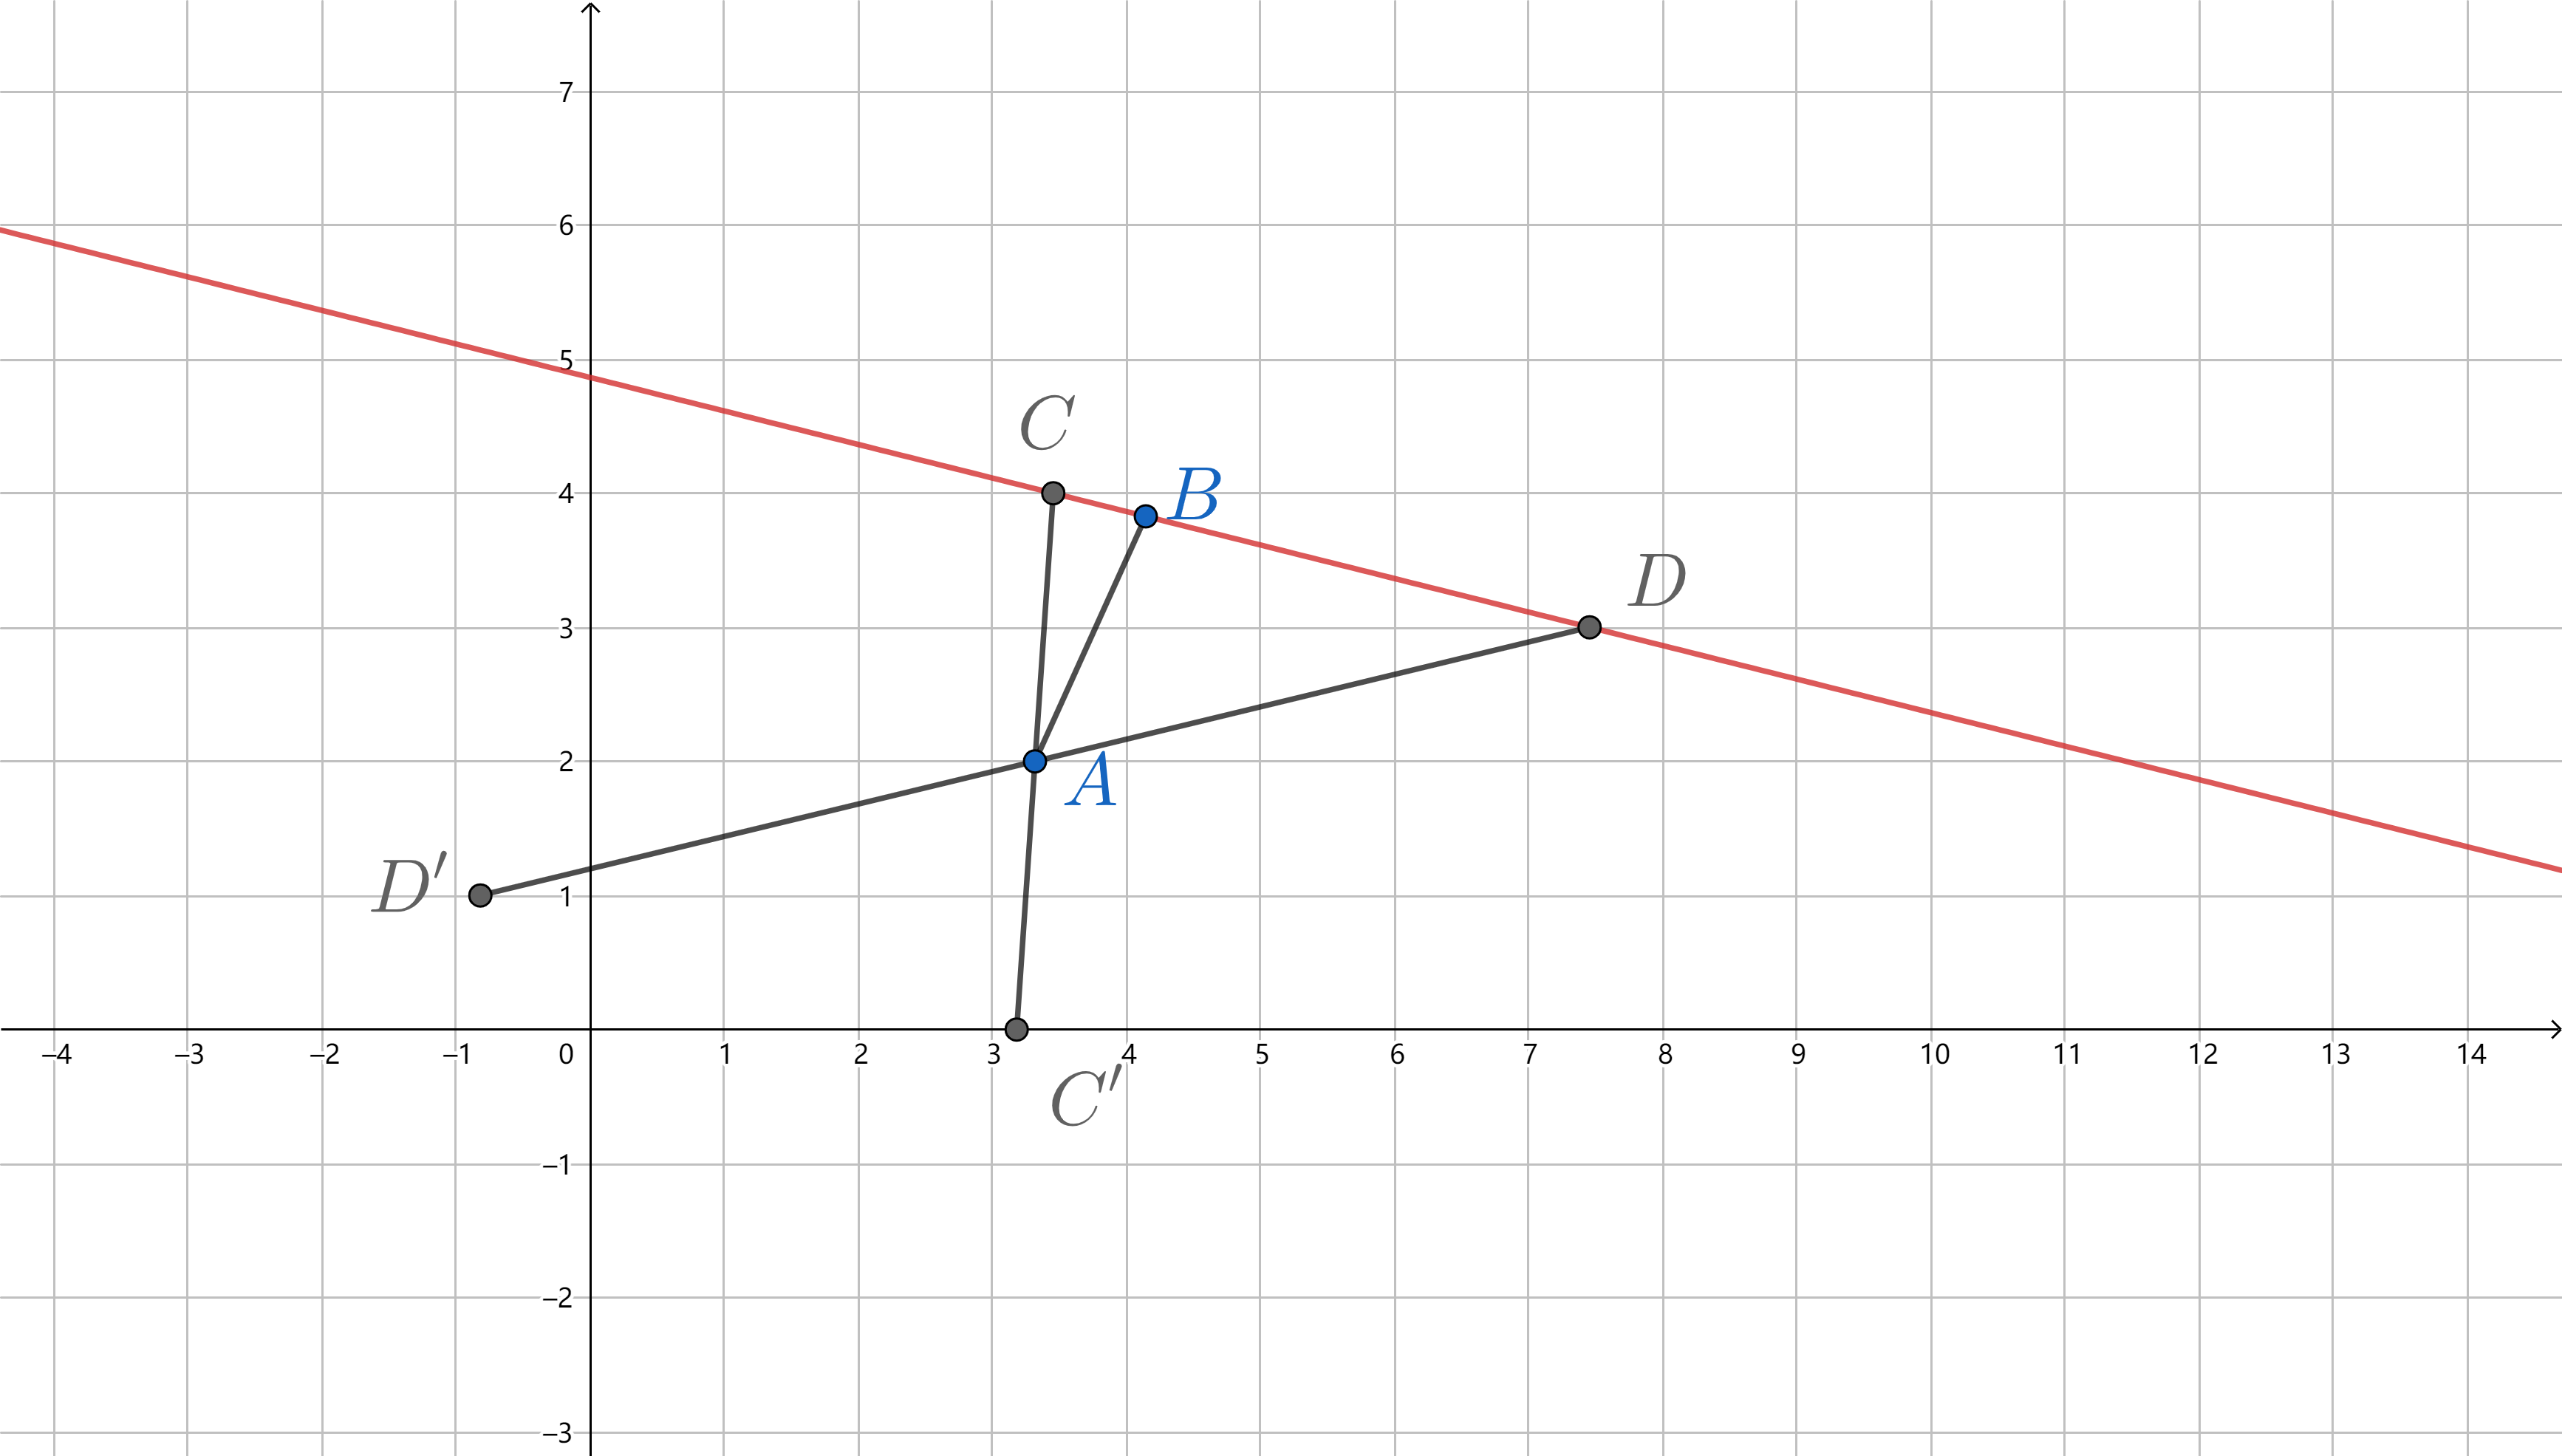
\includegraphics[width=5.76806in,height=3.27847in]{media/image32.png}

此时,我们连接 \(C^{'}D^{'}\),在延长线段 \(BA\) 交线段 \(C^{'}D^{'}\)
于 \(B^{'}\),\(AB^{'}\) 即为所求。

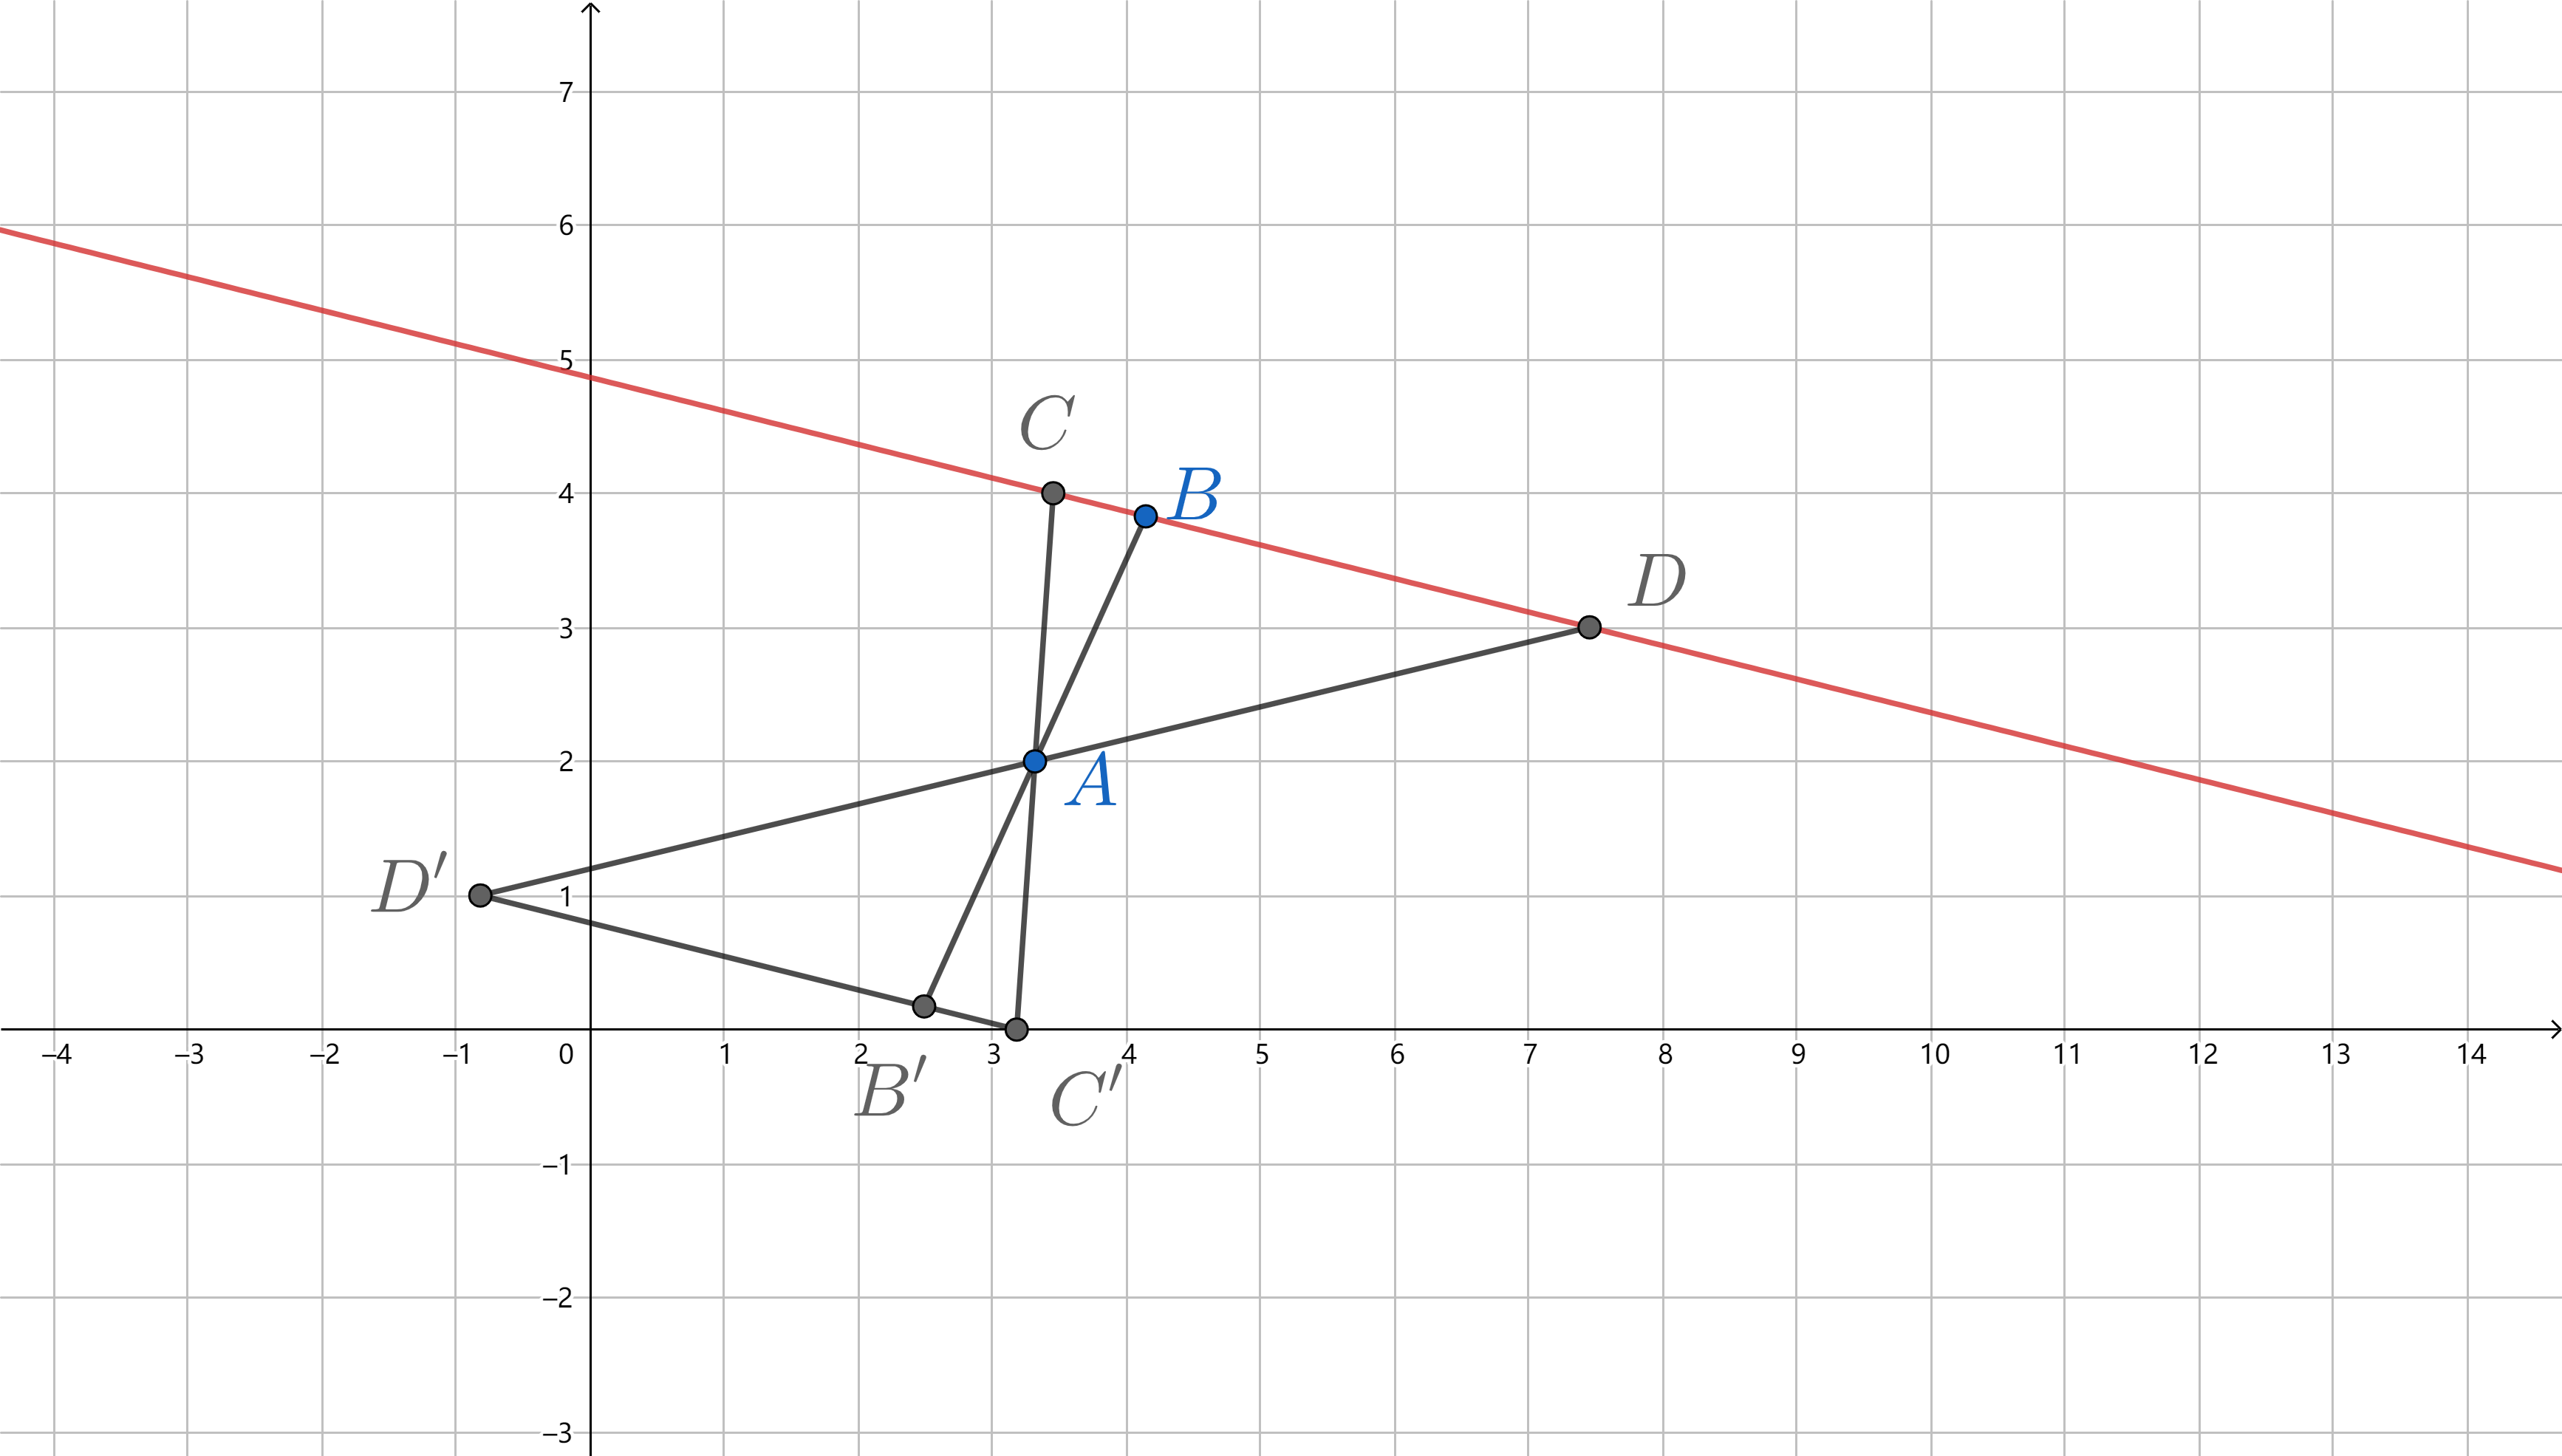
\includegraphics[width=5.76806in,height=3.27847in]{media/image33.png}

这个方法也可以推广到倍长至原线段的三倍,下面给出了三倍倍长的图,读者可以自行尝试理解。

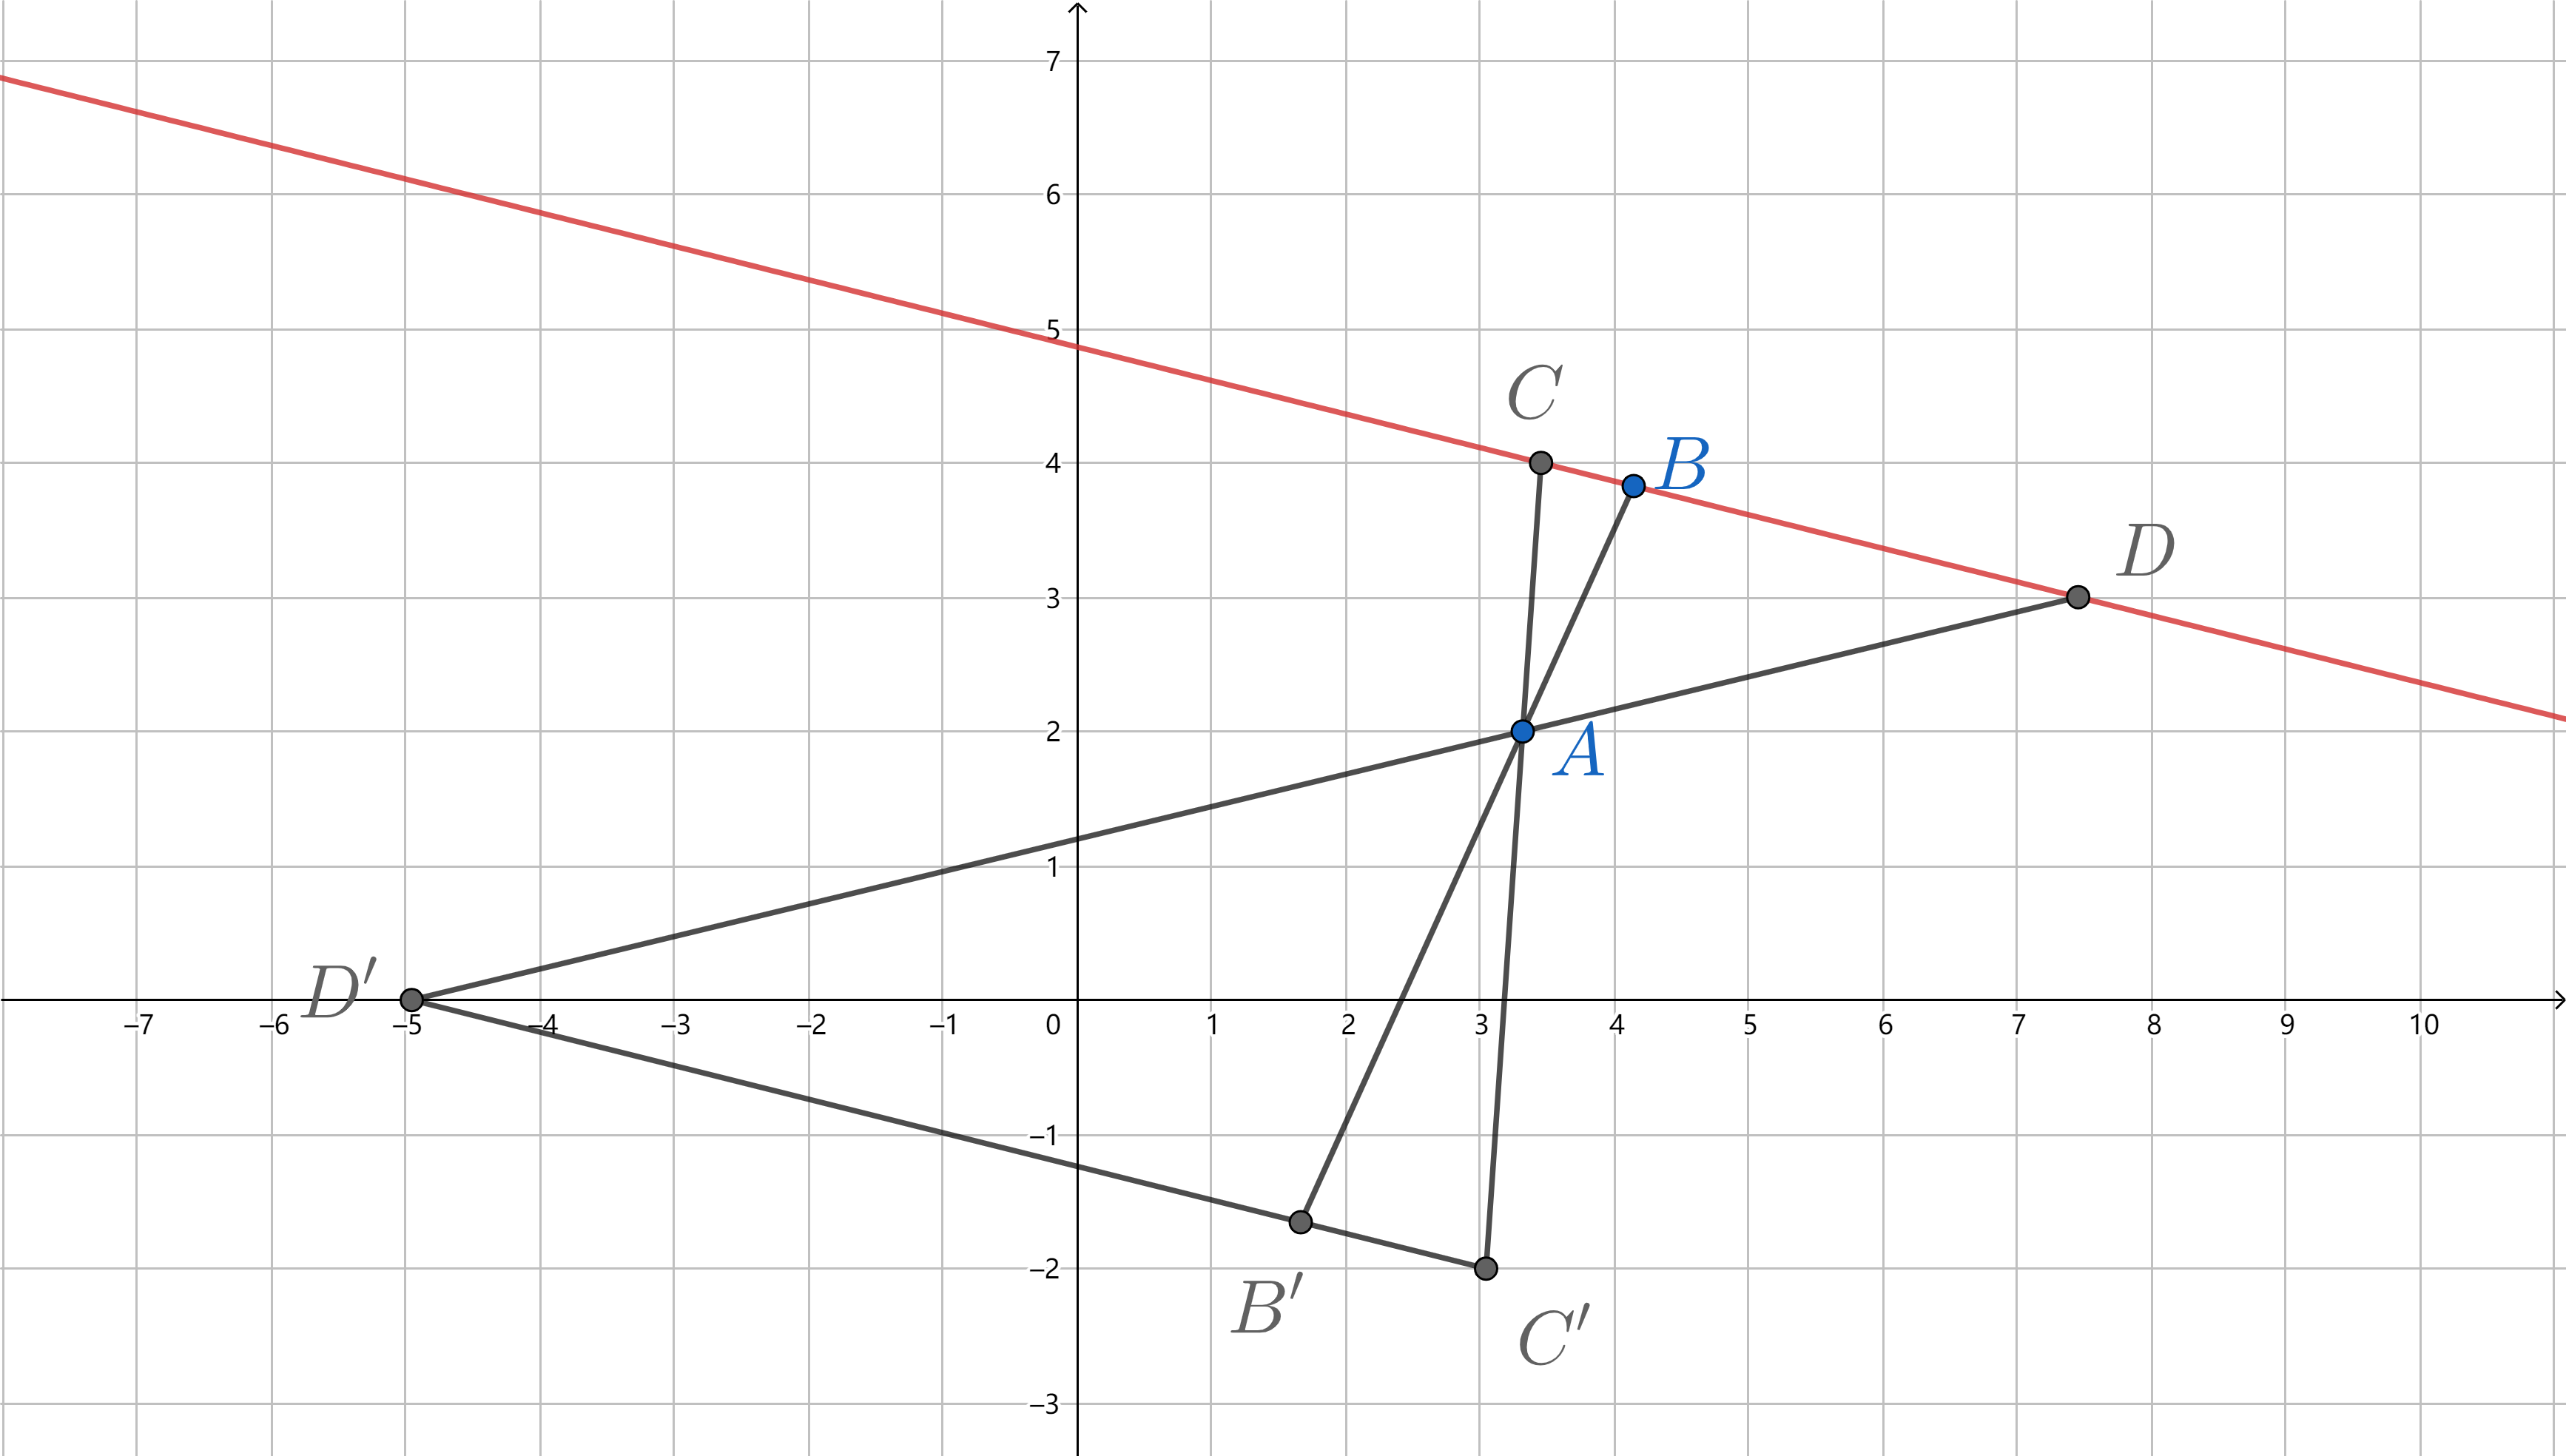
\includegraphics[width=5.76806in,height=3.27292in]{media/image34.png}

我们再看向自由端点方向倍长线段。此时的图与Wyc分线段定理的图几乎完全相同。

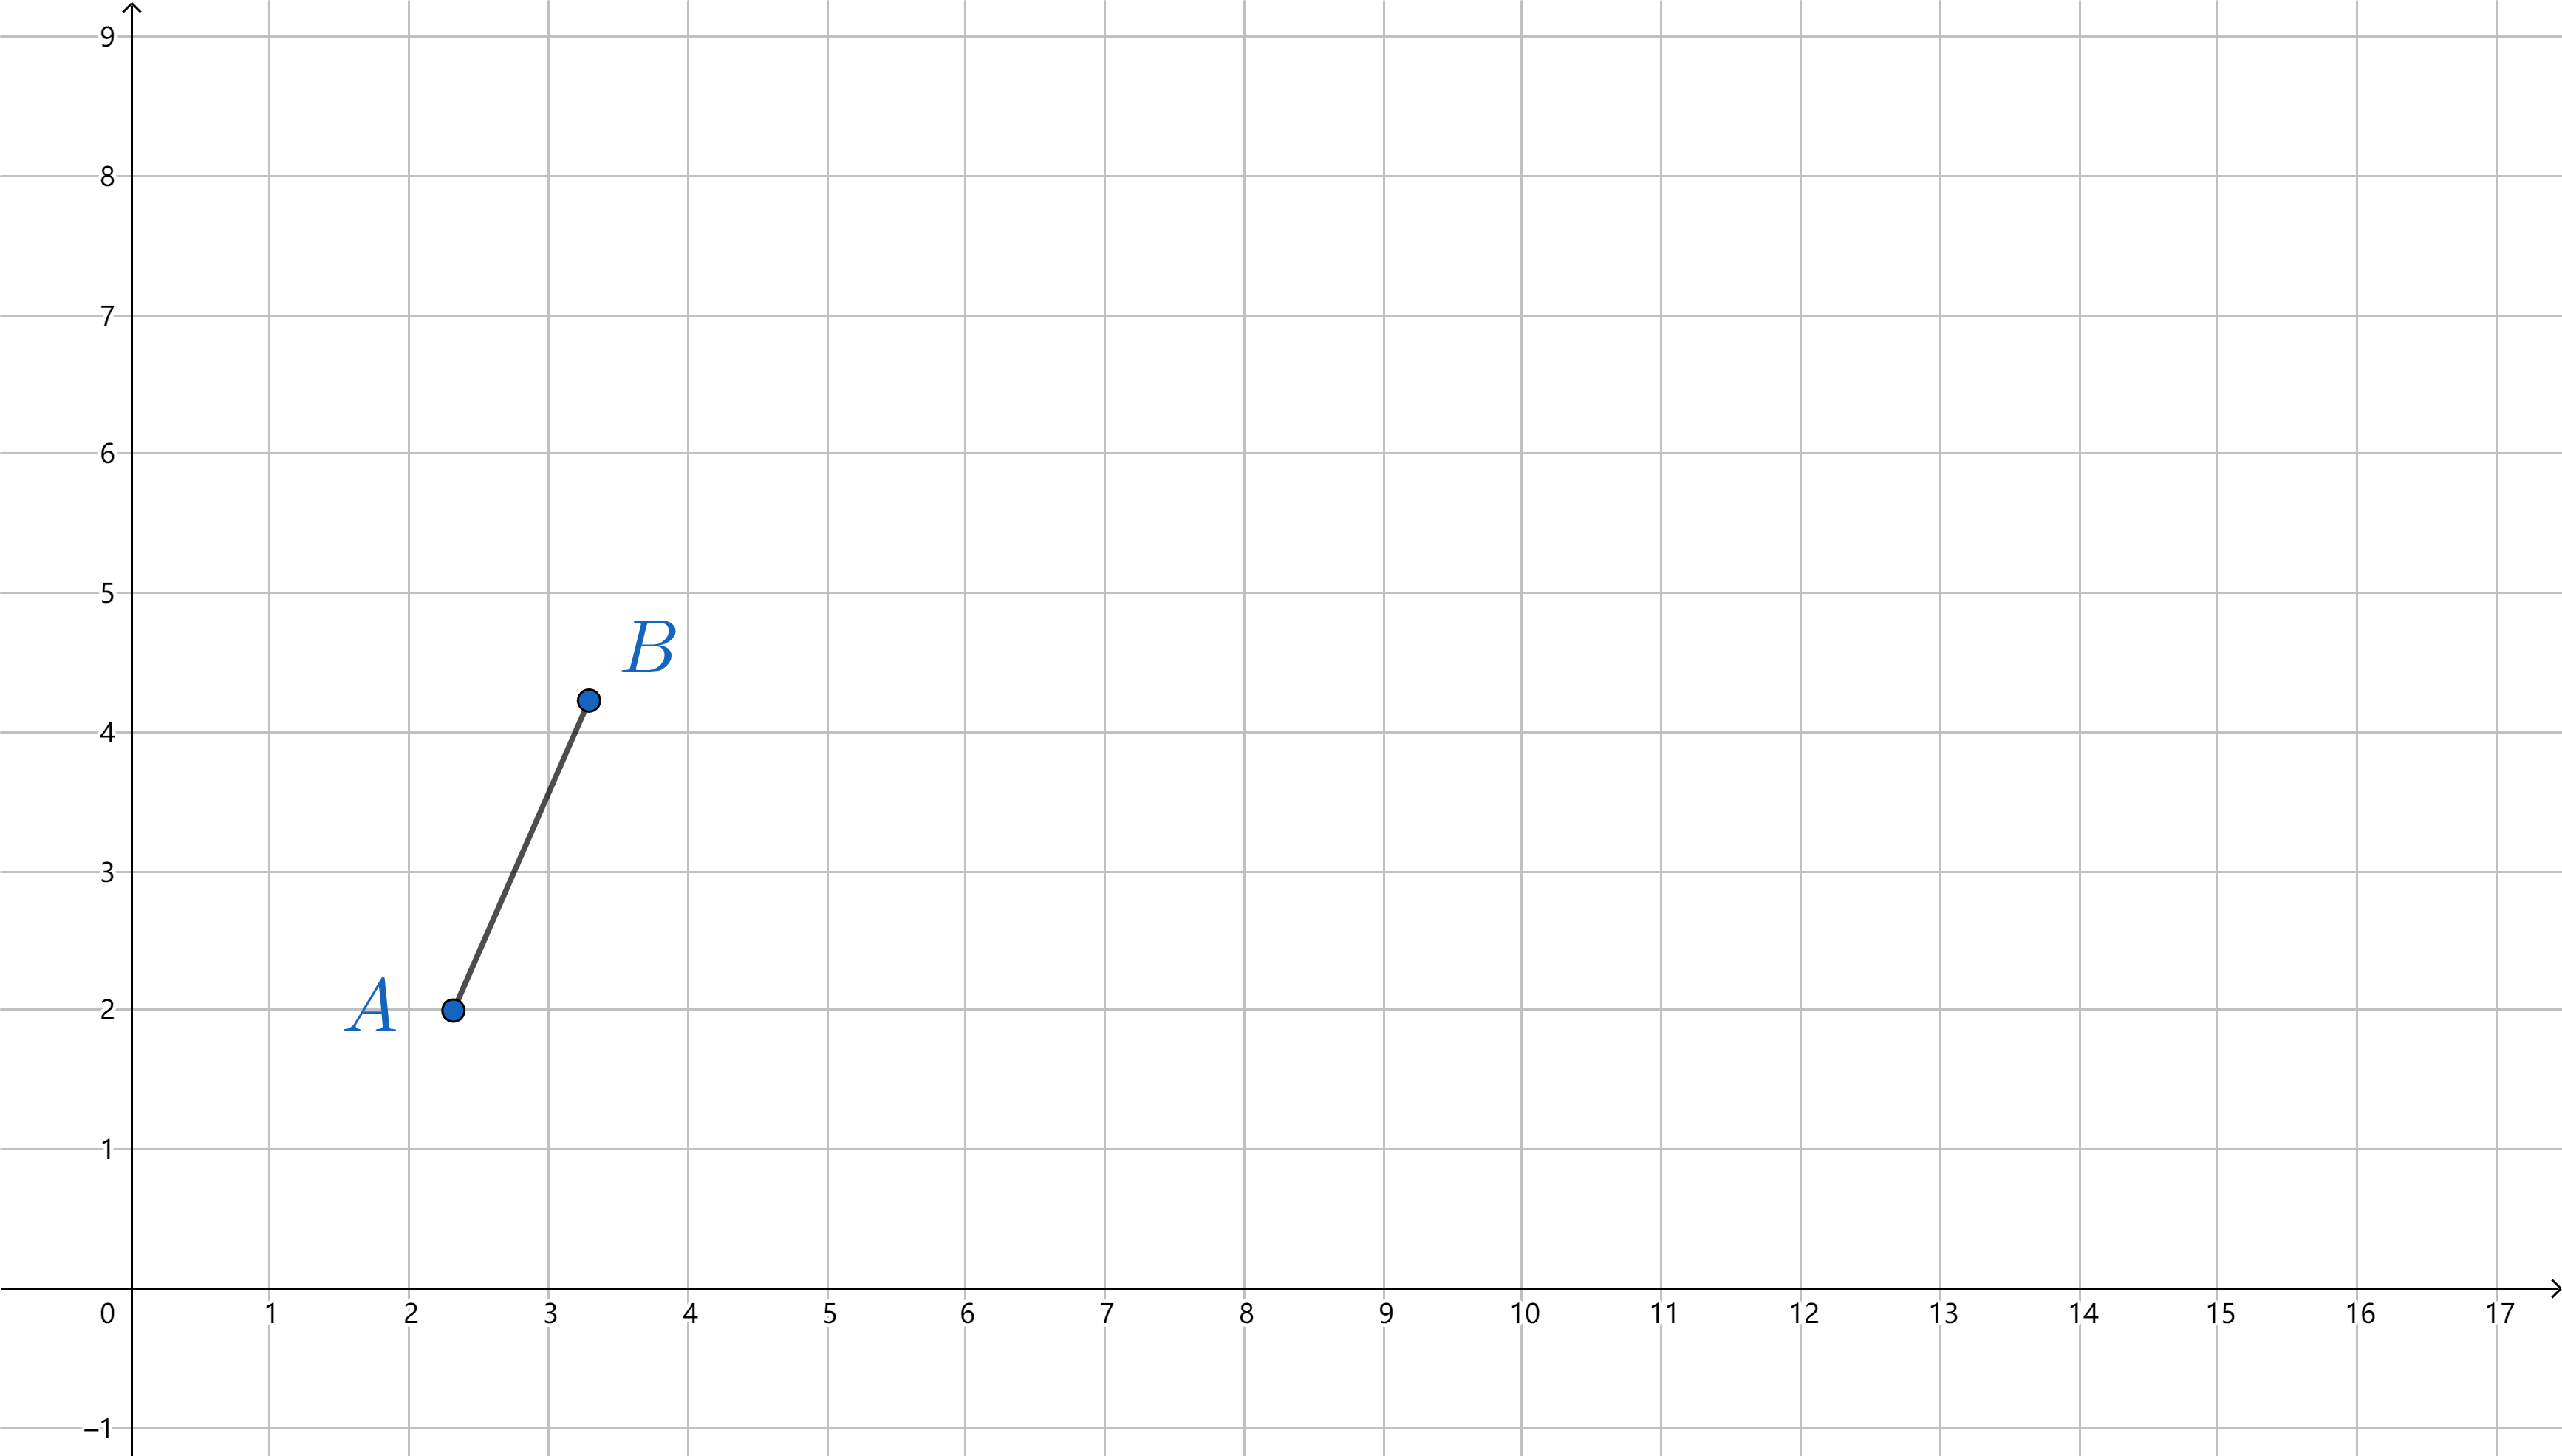
\includegraphics[width=5.76806in,height=3.27847in]{media/image35.png}

如图,\(A\) 在格线上,请在射线 \(AB\) 上找到点 \(M\) 使得 \(AB = BM\)。

我们还是需要通过构造中位线的方法来解决这个问题。

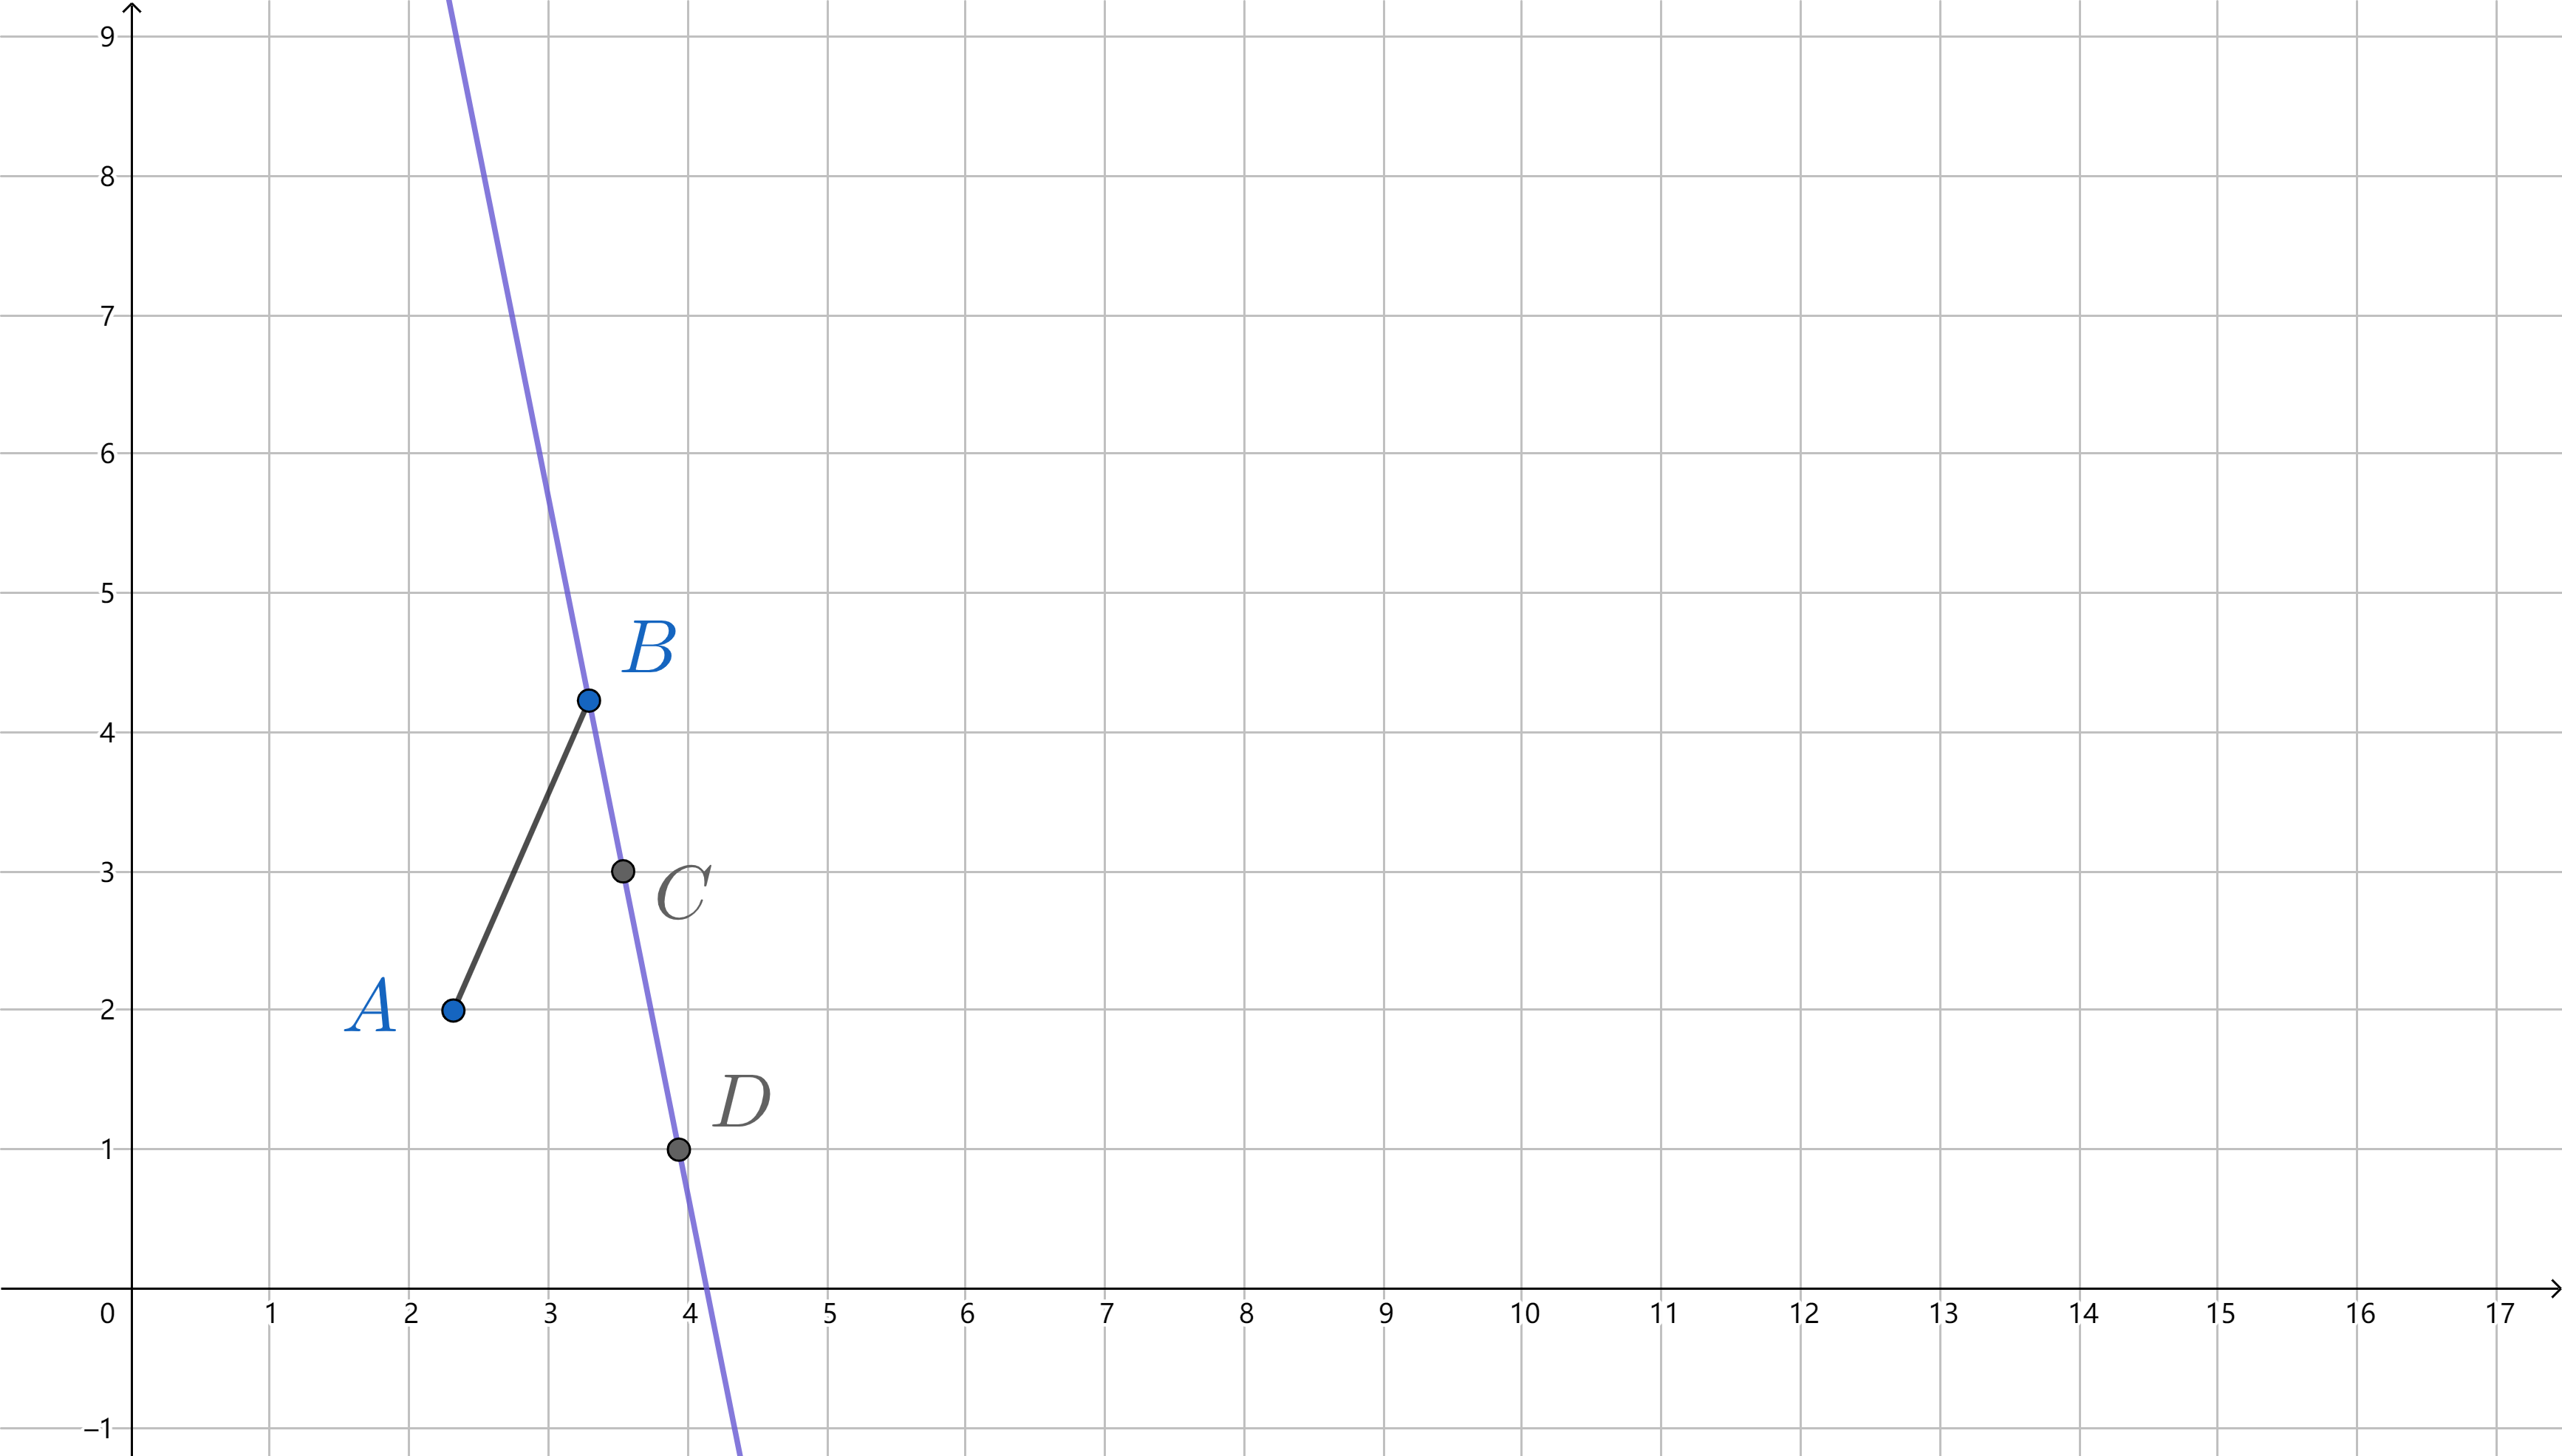
\includegraphics[width=5.76806in,height=3.27847in]{media/image36.png}

如图,过 \(B\) 作一条合适的直线,取这条直线与两条水平格线的交点,分别为
\(C\) 和 \(D\)。通过 \(A\),\(C\),\(D\)
都在水平格线上这一条件,我们可以很简单地倍长线段 \(AC\) 和线段 \(AD\)。

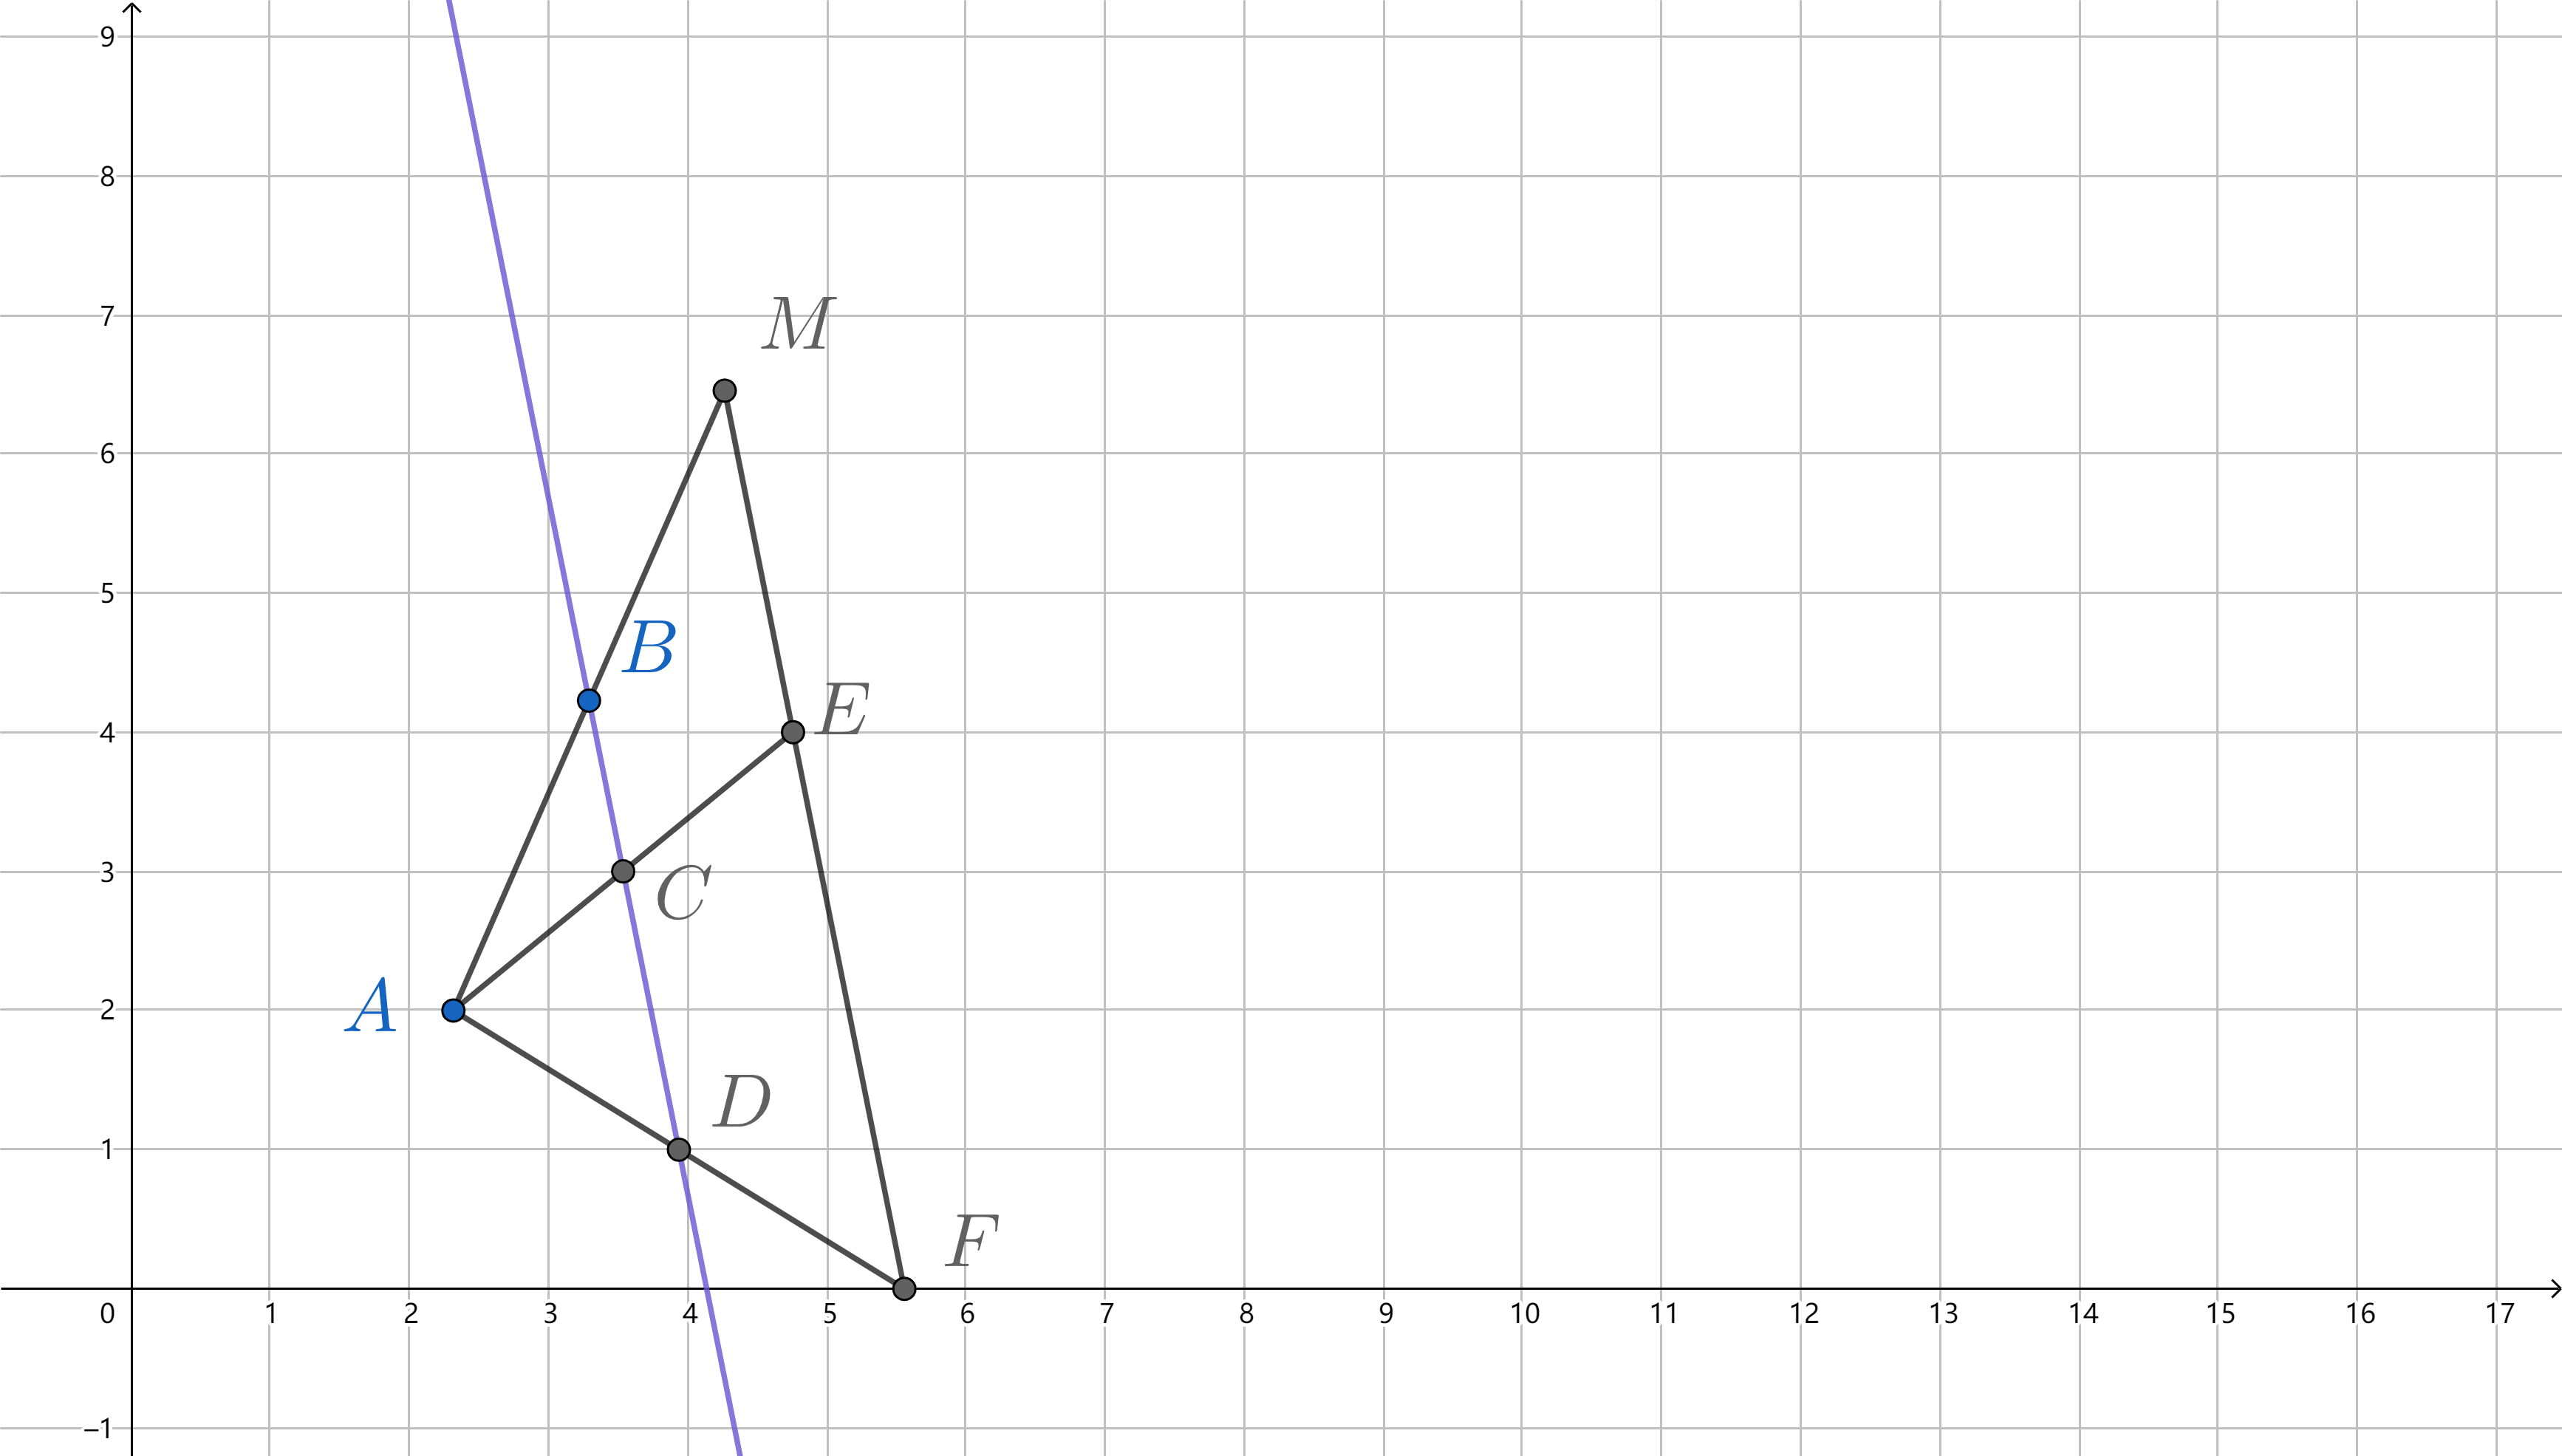
\includegraphics[width=5.76806in,height=3.27847in]{media/image37.png}

如图,倍长线段 \(AC\) 至 \(E\),倍长线段 \(AD\) 至 \(F\),连接 \(FE\)
并延长交 \(AB\) 延长线于 \(M\),\(M\) 即为所求。

同样地,我们可以把 \(AB\)
倍长至原来的三倍或四倍。下面给出了倍长至原线段三倍的图。

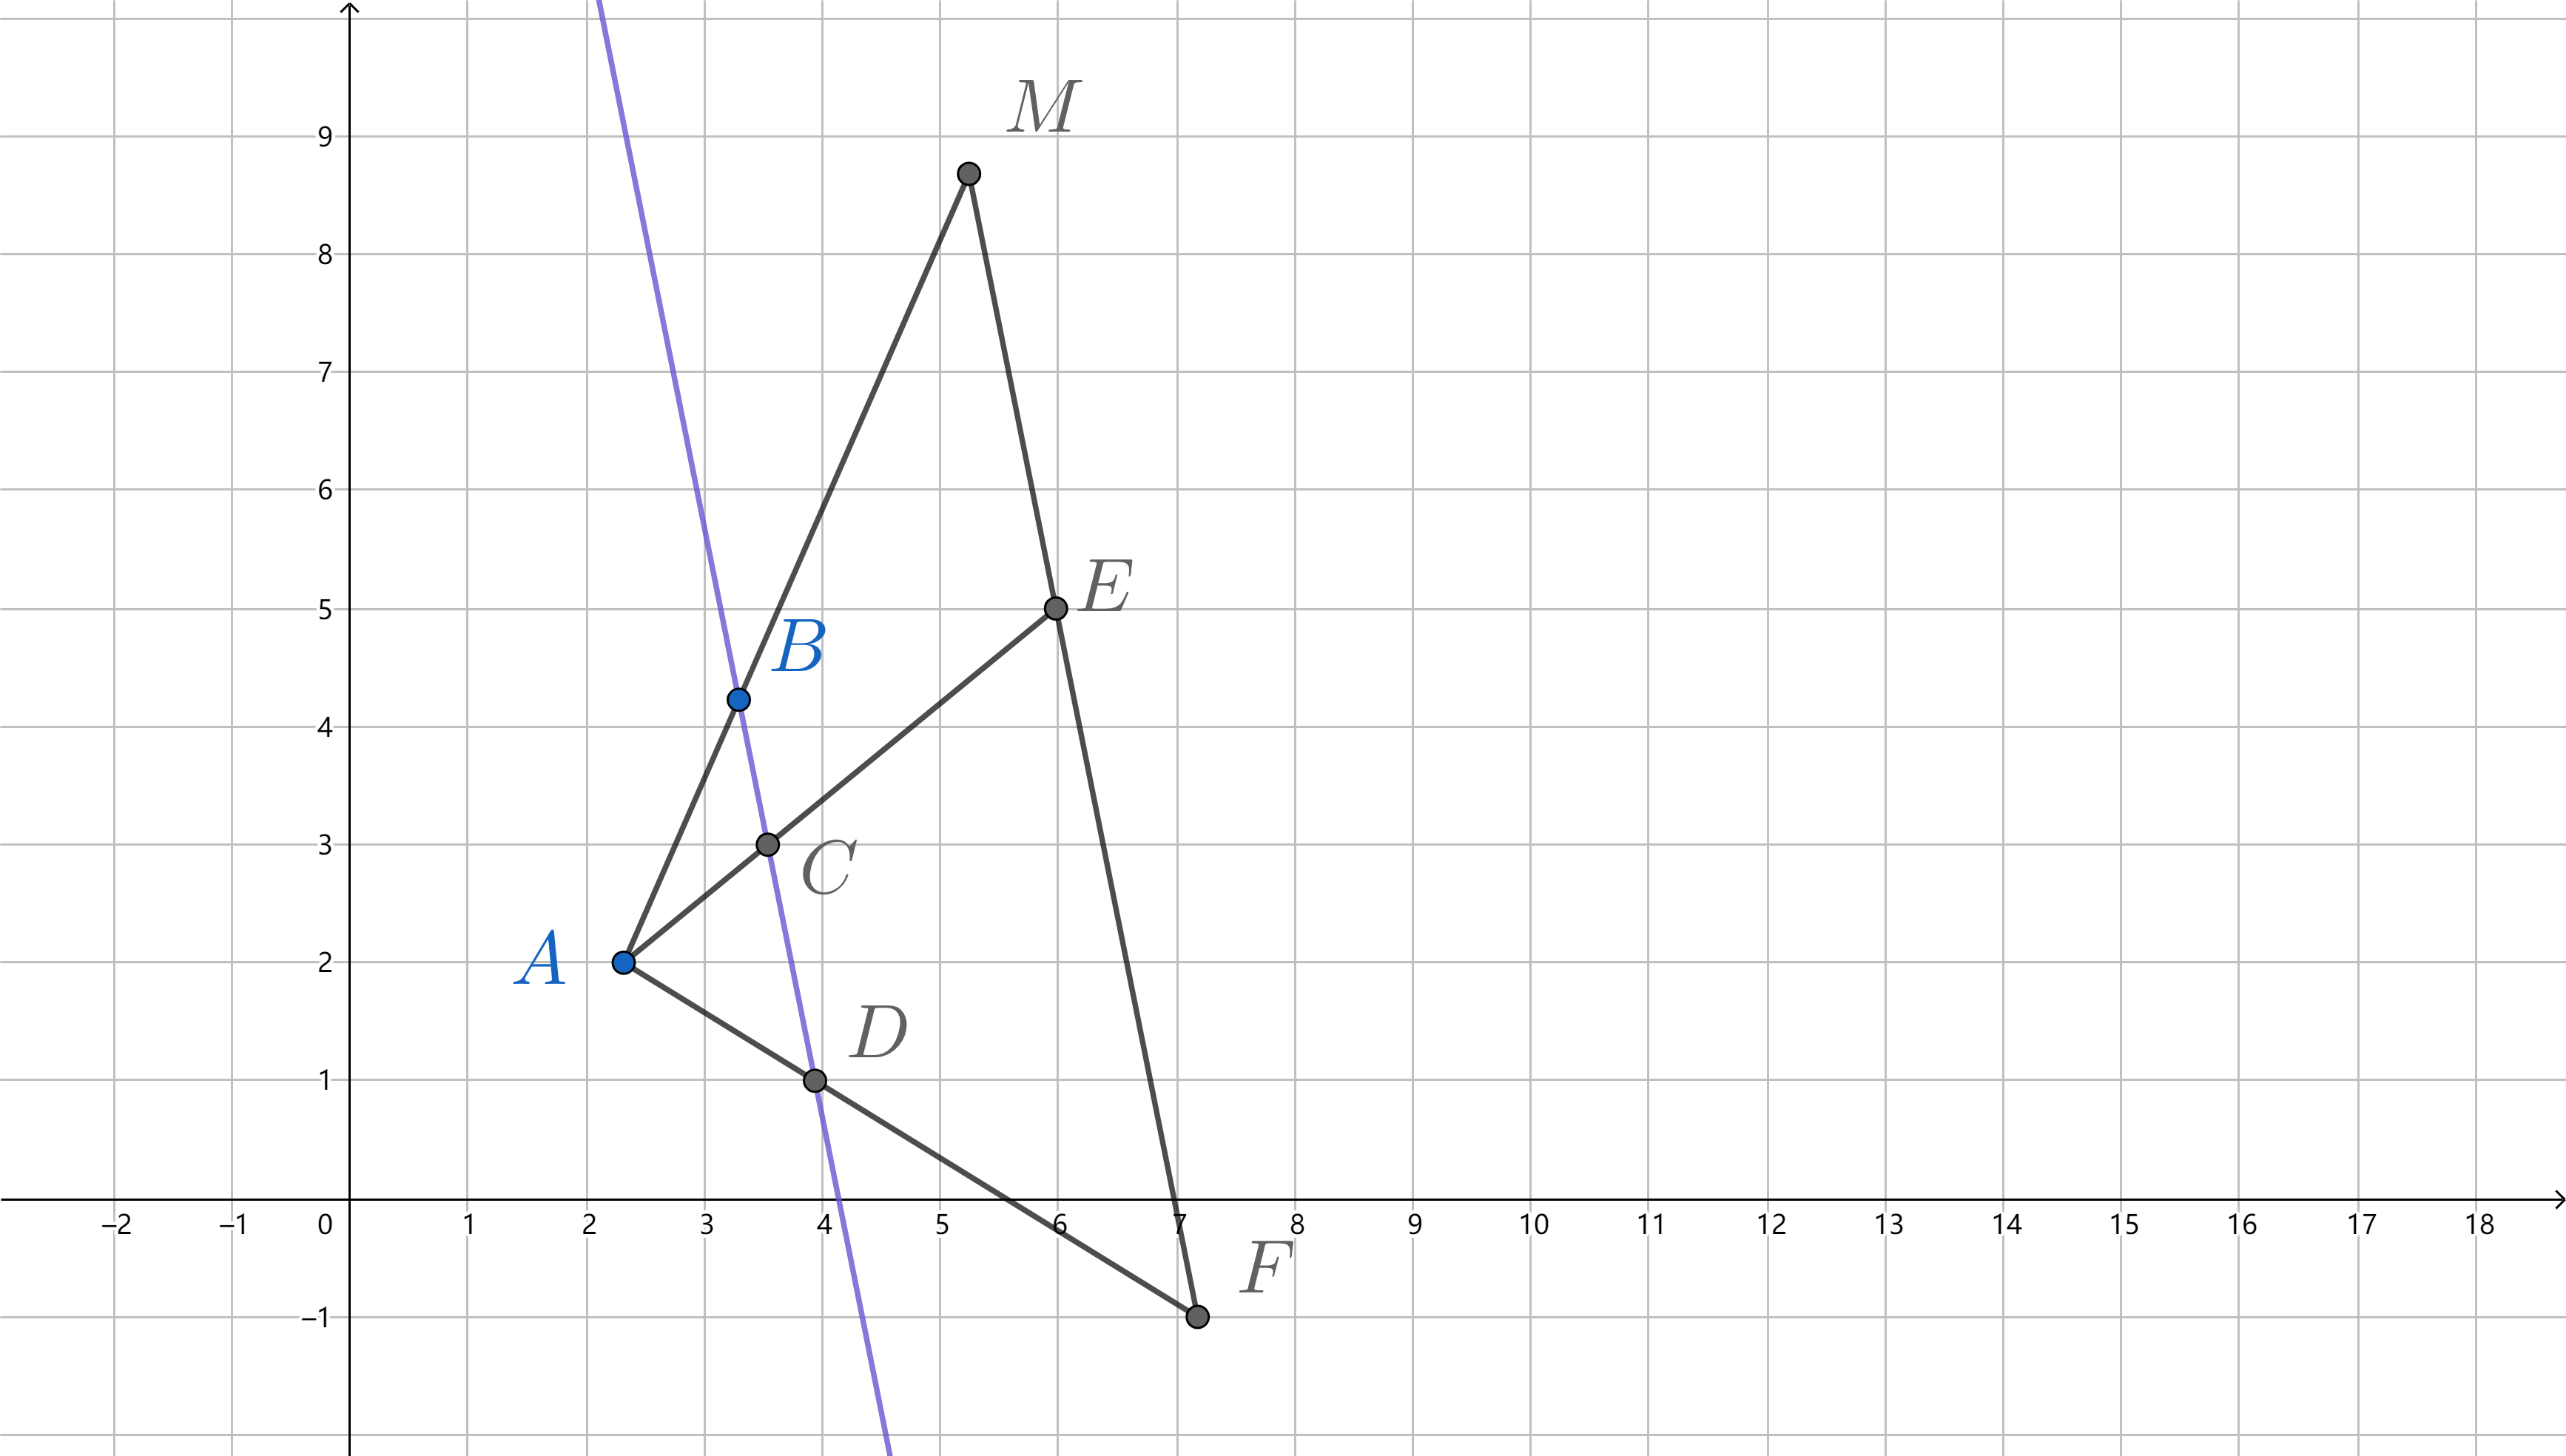
\includegraphics[width=5.76806in,height=3.27292in]{media/image38.png}

\hypertarget{wycux500dux957fux7ebfux6bb5ux5b9aux7406-wycs-segment-multiplication-theoremux5b9aux7406-3.6}{%
\subsection{Wyc倍长线段定理 Wyc's Segment Multiplication Theorem(定理
3.6)}\label{wycux500dux957fux7ebfux6bb5ux5b9aux7406-wycs-segment-multiplication-theoremux5b9aux7406-3.6}}

\textbf{【提出者】}王宇辰(向自由端倍长)、翟悦凯(向格线端点倍长)

当一条线段的一个端点在格线上时,可以用比倍长线段定理(定理
3.1.3)更简单的方法倍长它。

我们现在要考虑倍长任意线段的方法了。我们来看图:

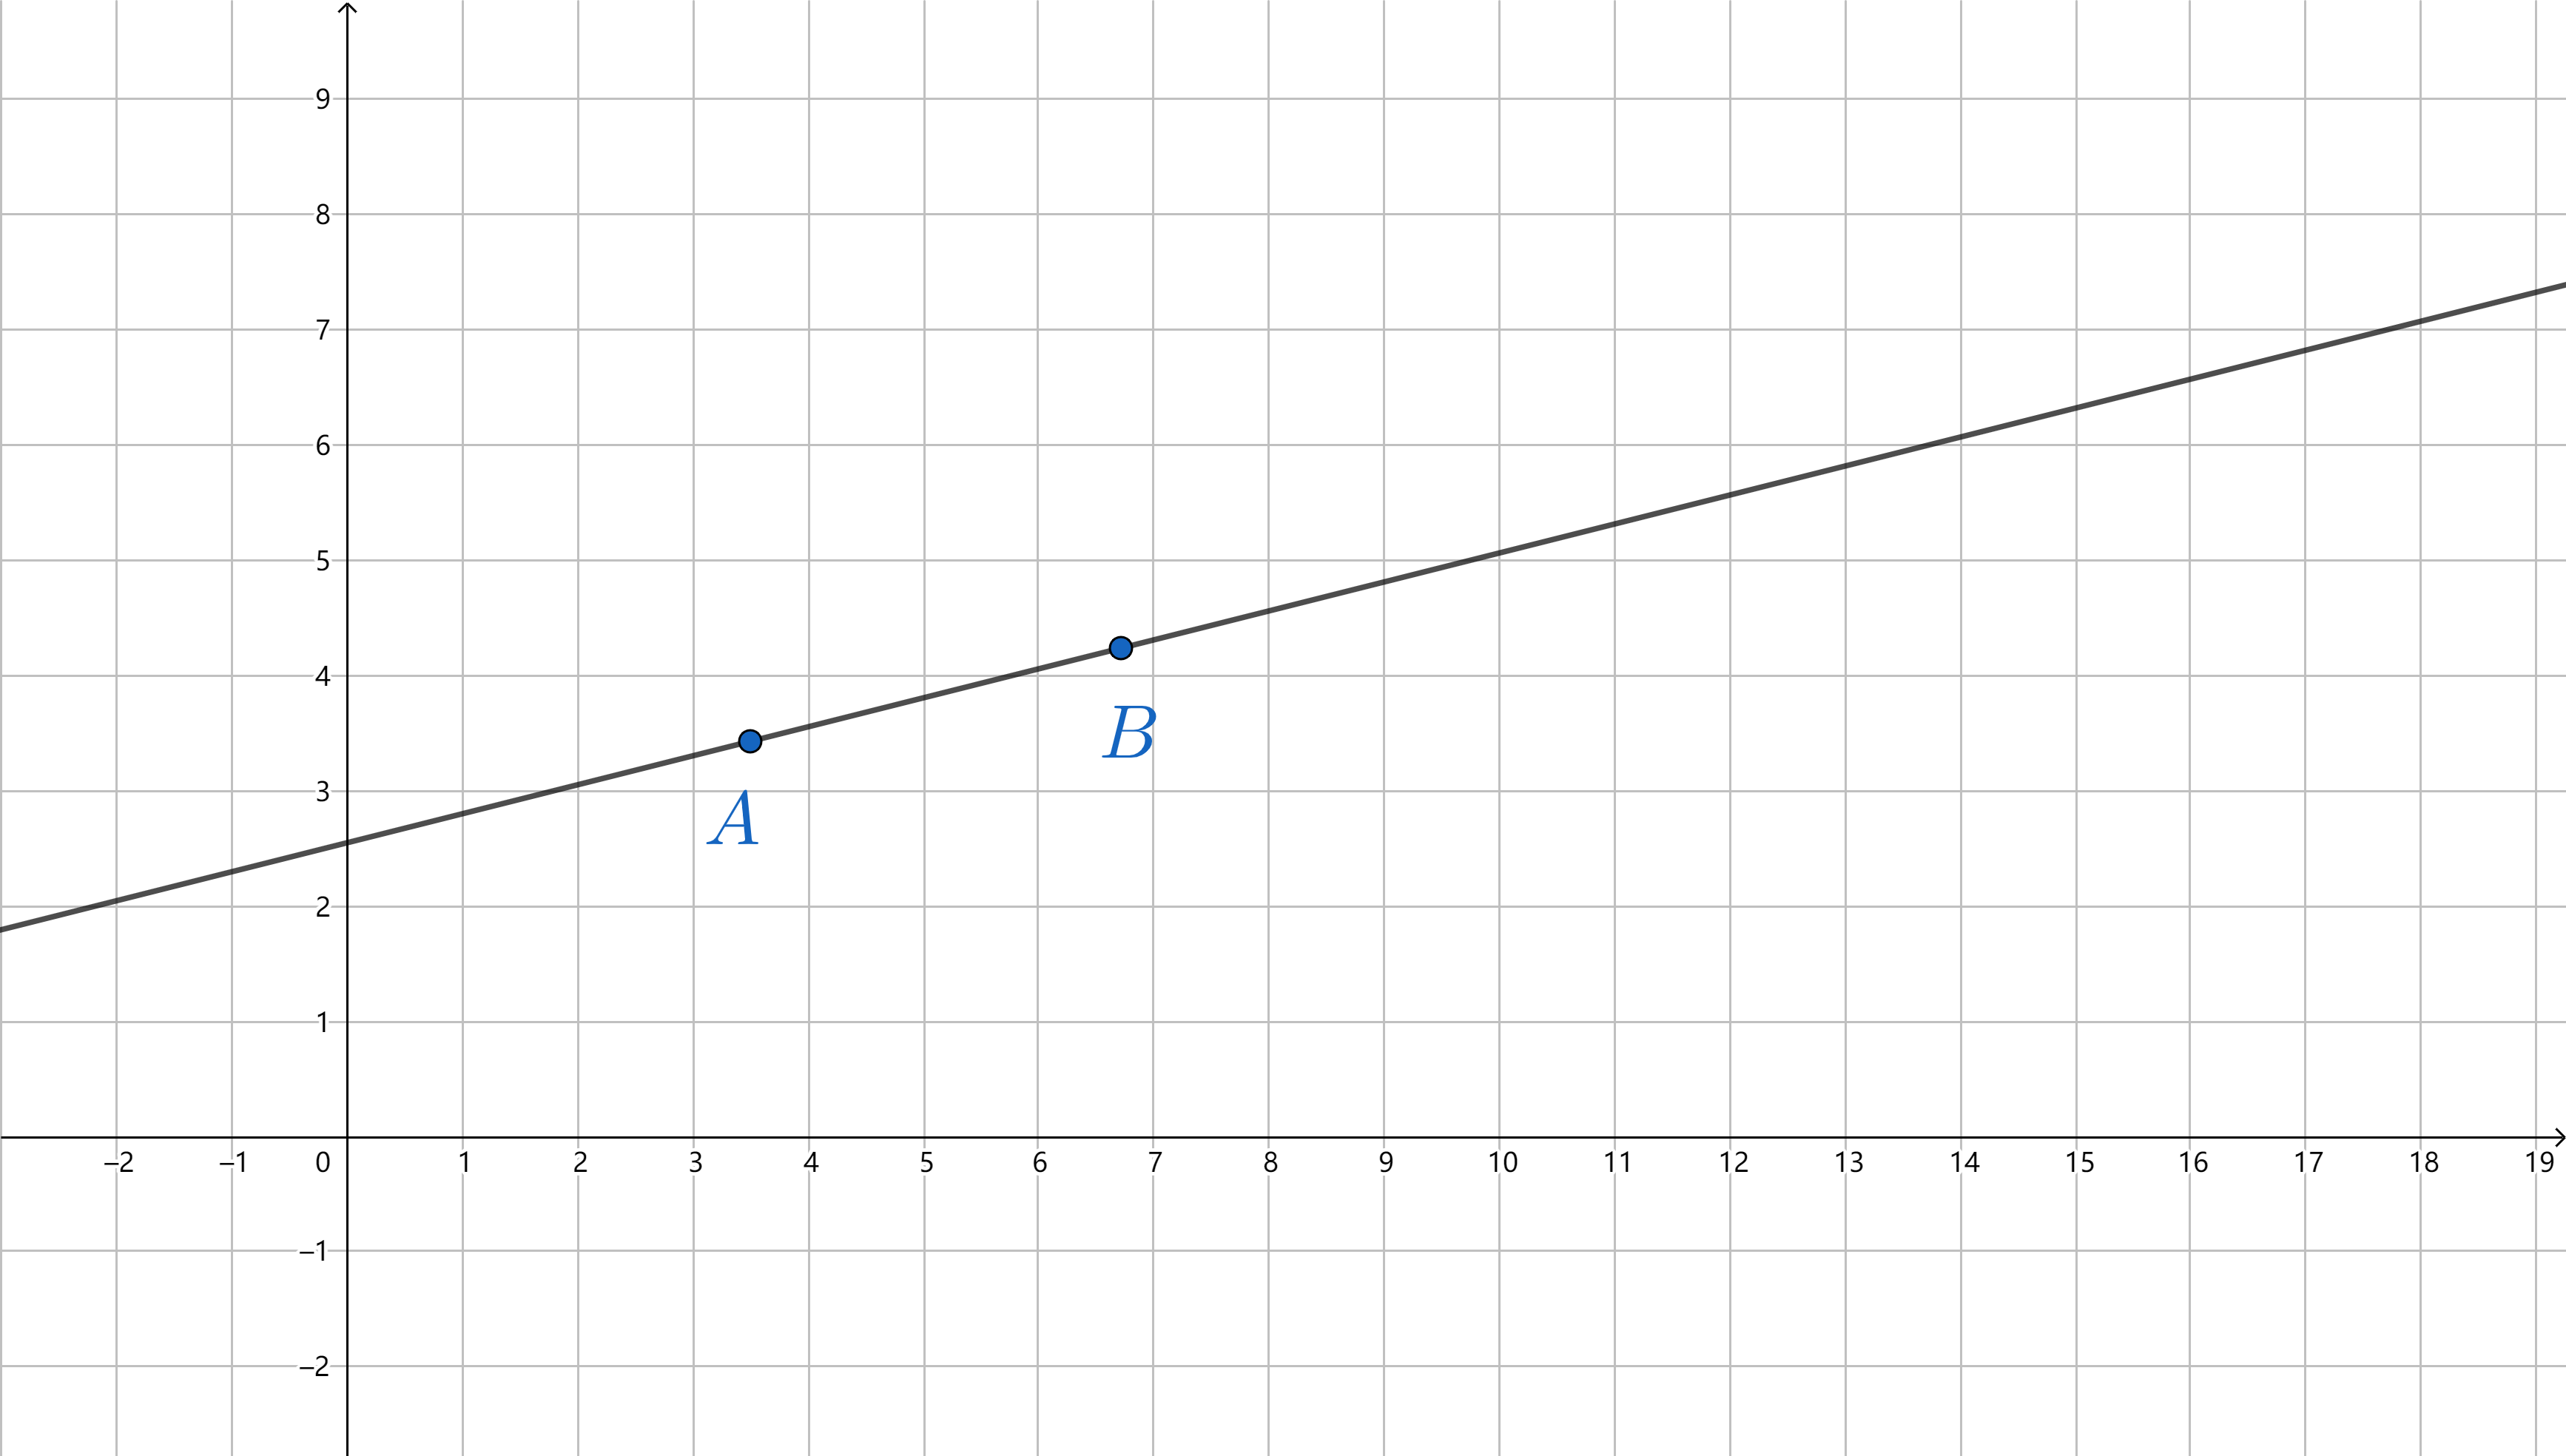
\includegraphics[width=5.76806in,height=3.27292in]{media/image39.png}

如图,\(A\),\(B\) 为任意点,请在直线 \(AB\) 上取点 \(M\) 使得
\(AB = BM\),其中 \(A\),\(M\) 不重合。

我们需要再次通过构造中位线或相似的方法解决这个问题。

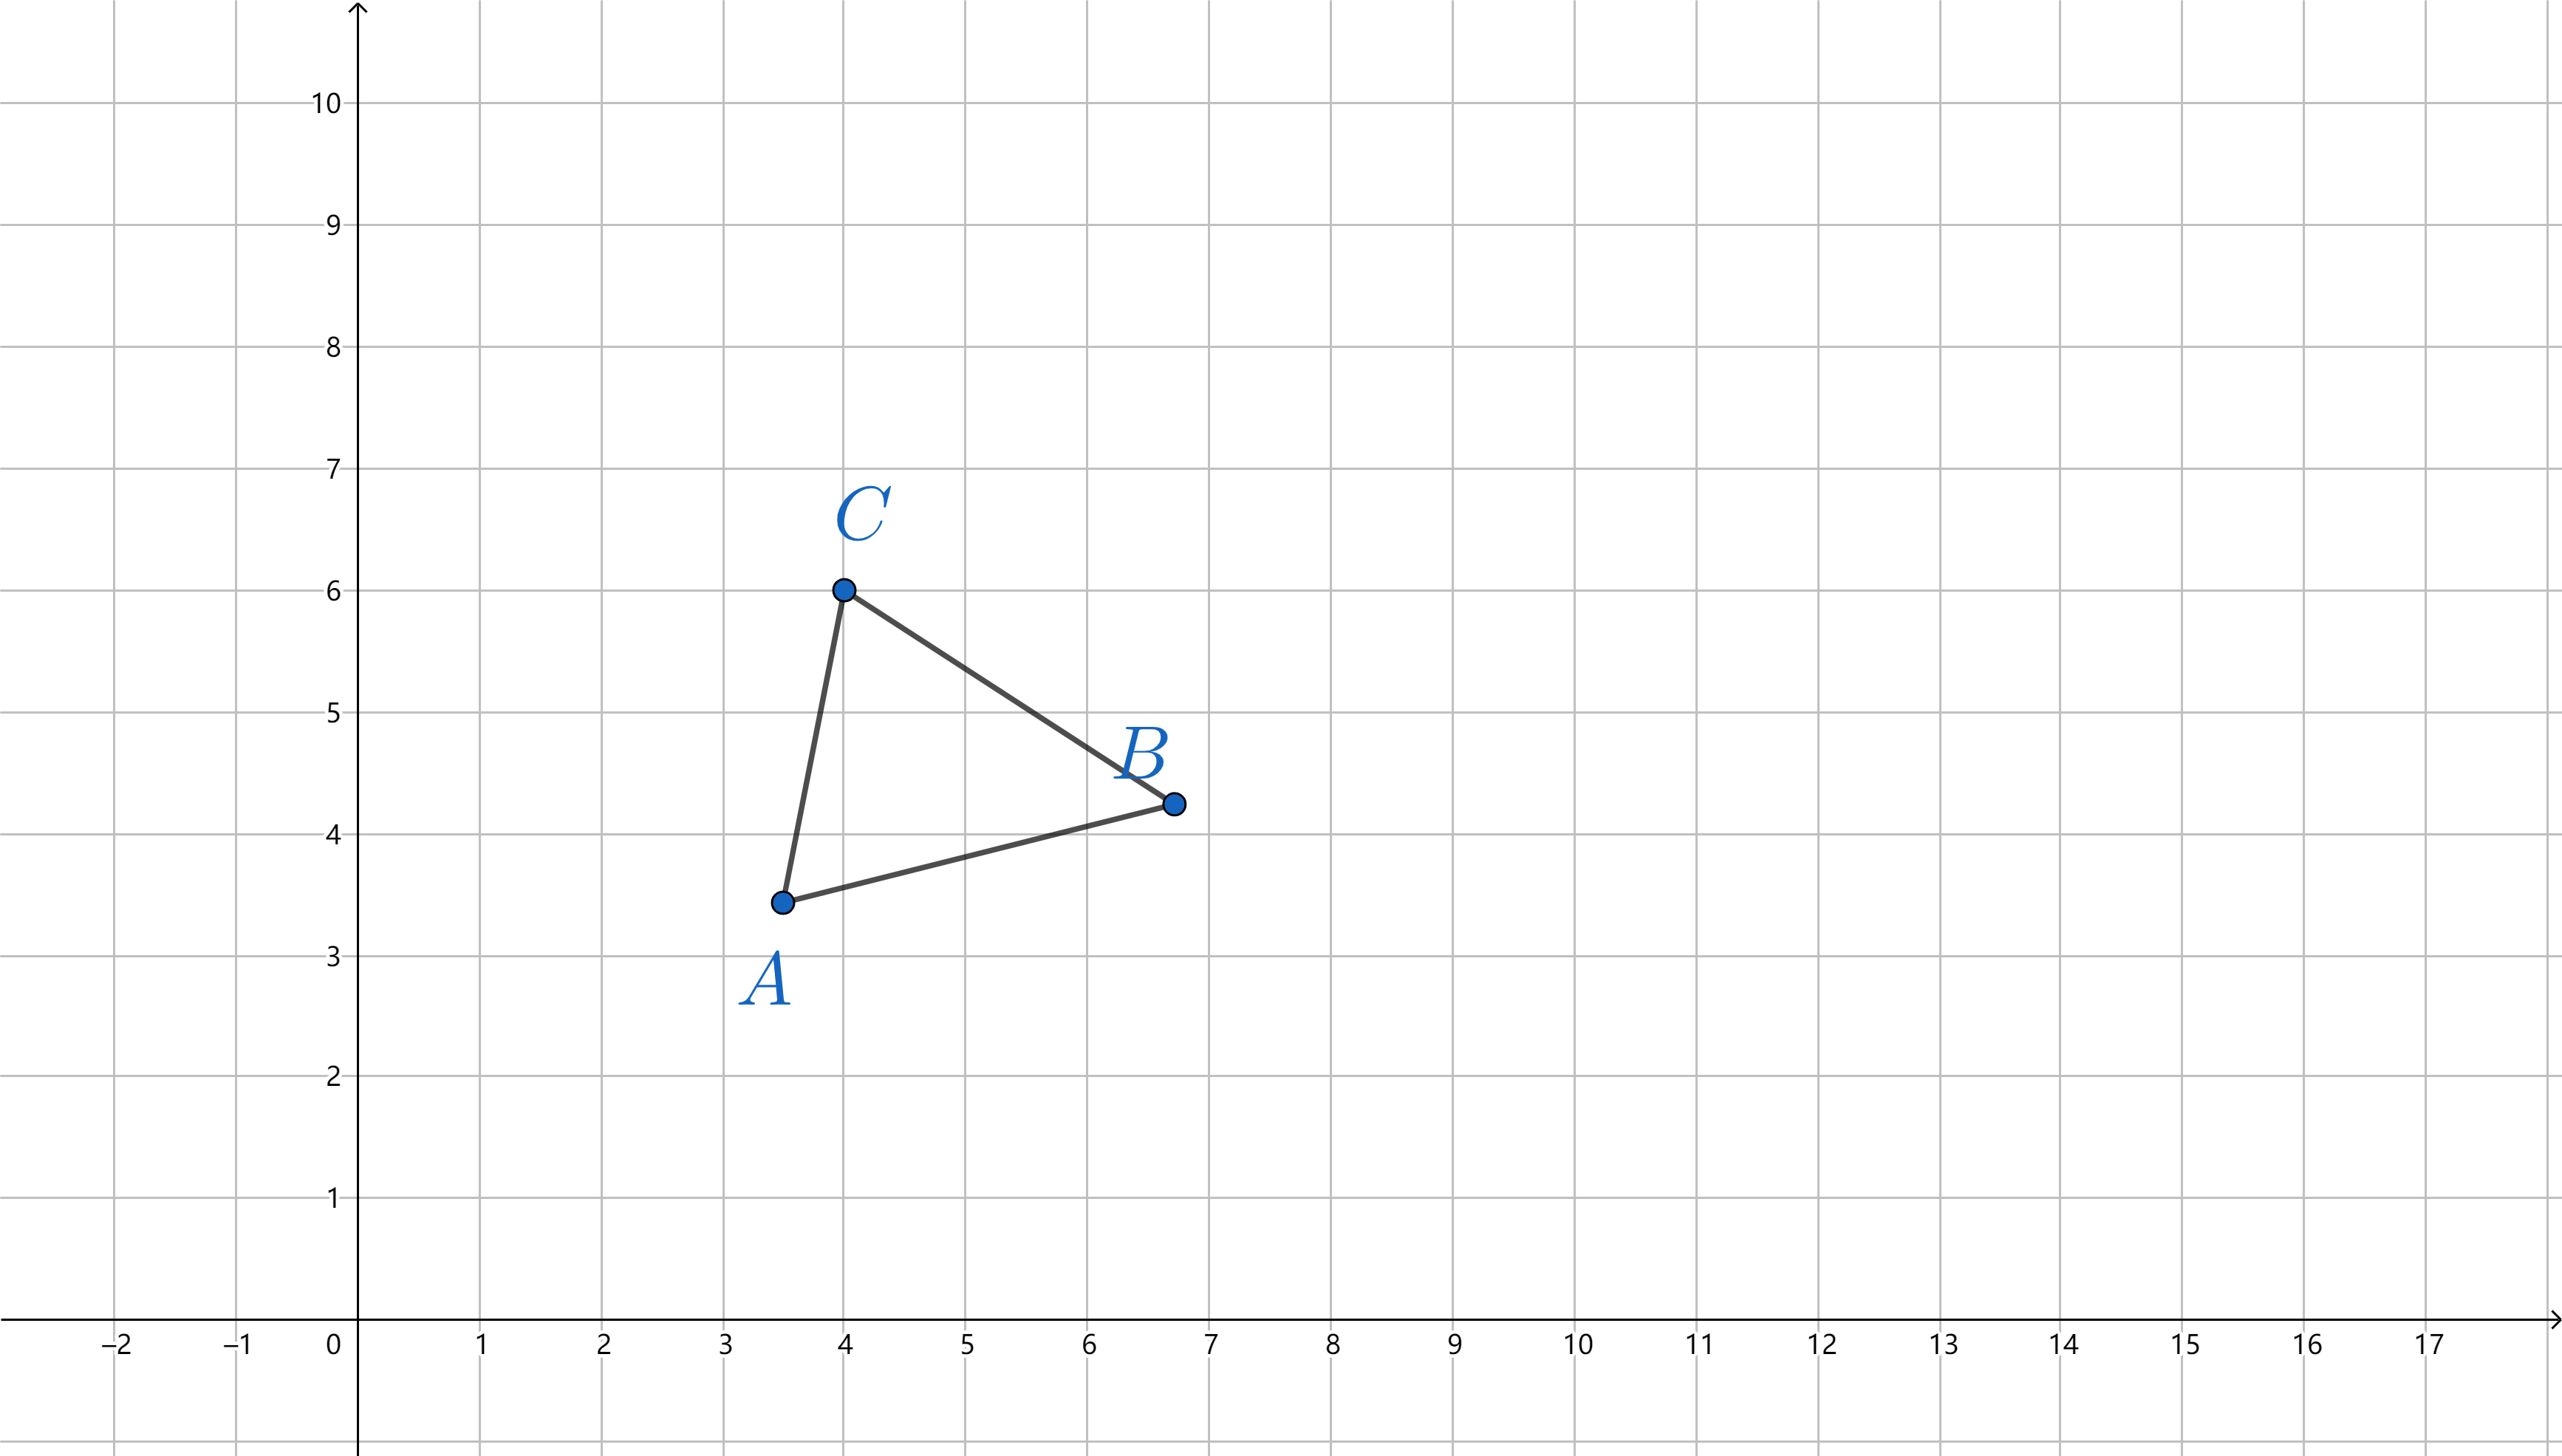
\includegraphics[width=5.76806in,height=3.27847in]{media/image40.png}

如图,我们选择格点 \(C\),连接 \(AC\)、\(BC\)。如果我们能把 \(AC\)
倍长至 \(N\),再过 \(N\) 作 \(BC\) 的平行线交射线 \(AB\) 于 \(M\),\(M\)
即为所求。我们可以来尝试一下。

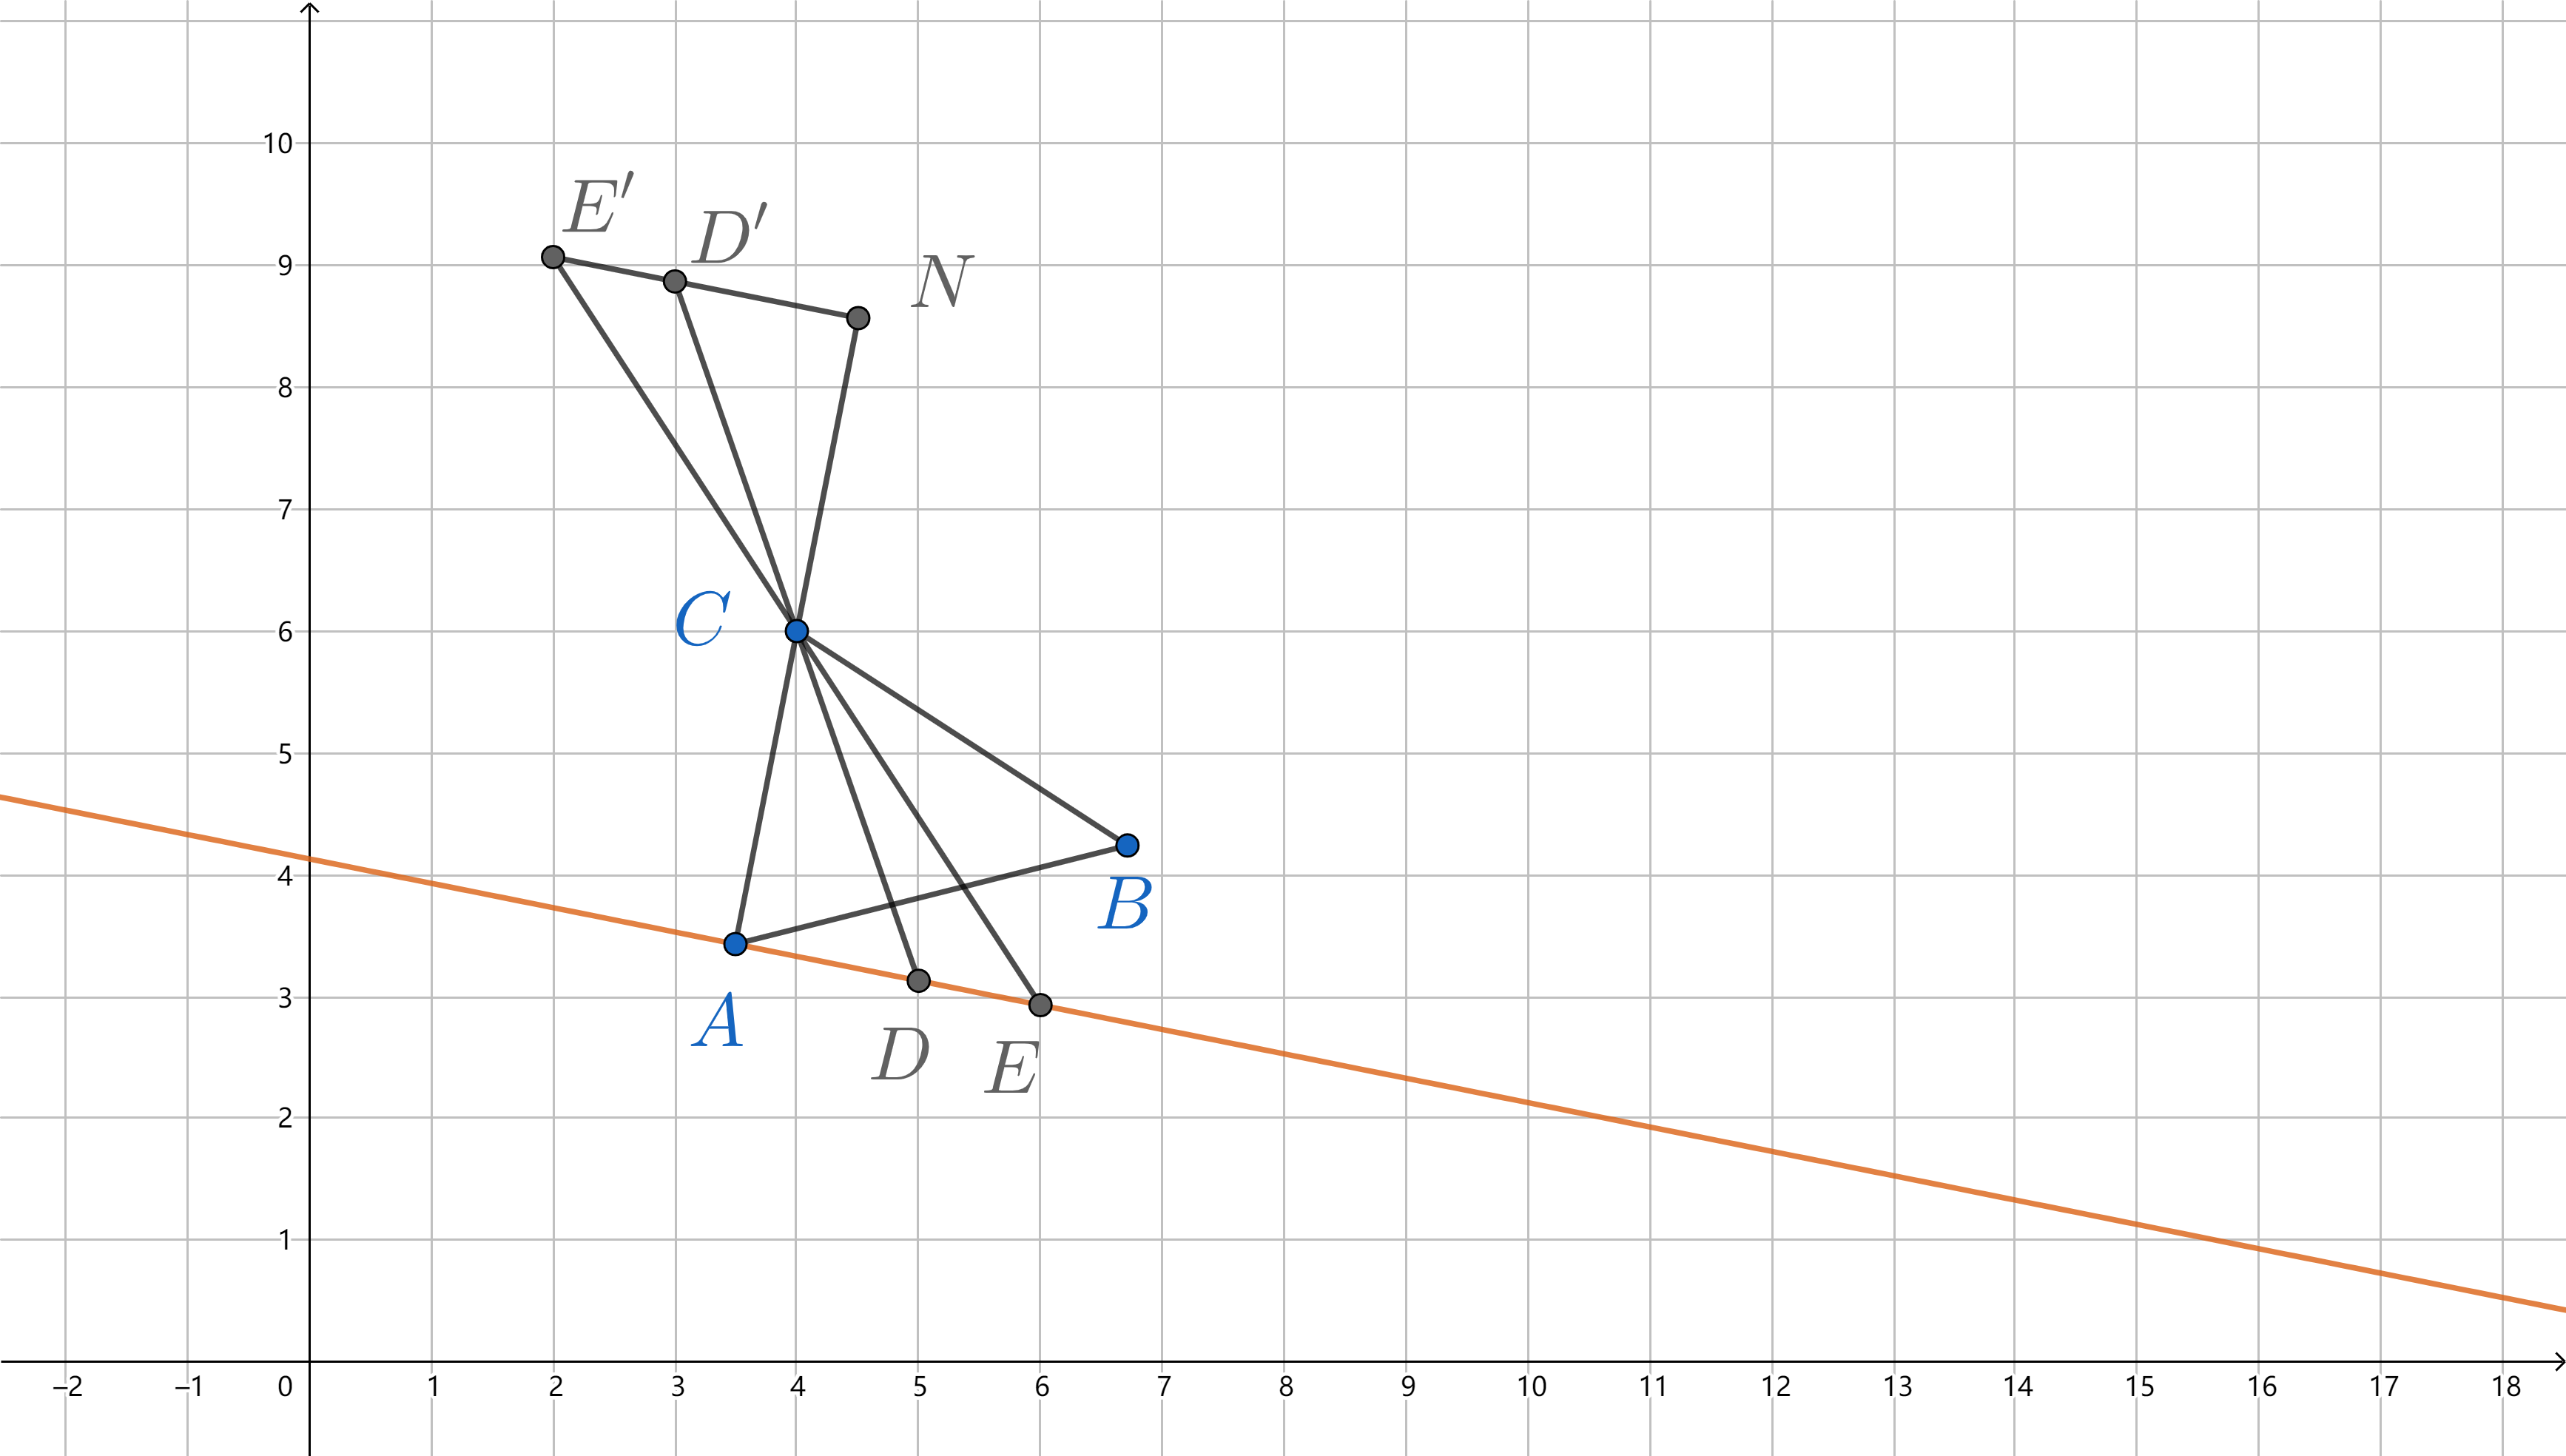
\includegraphics[width=5.76806in,height=3.27292in]{media/image41.png}

如图,我们把 \(AC\) 倍长到了 \(N\)。下面我们要过 \(N\) 作 \(BC\)
的平行线。

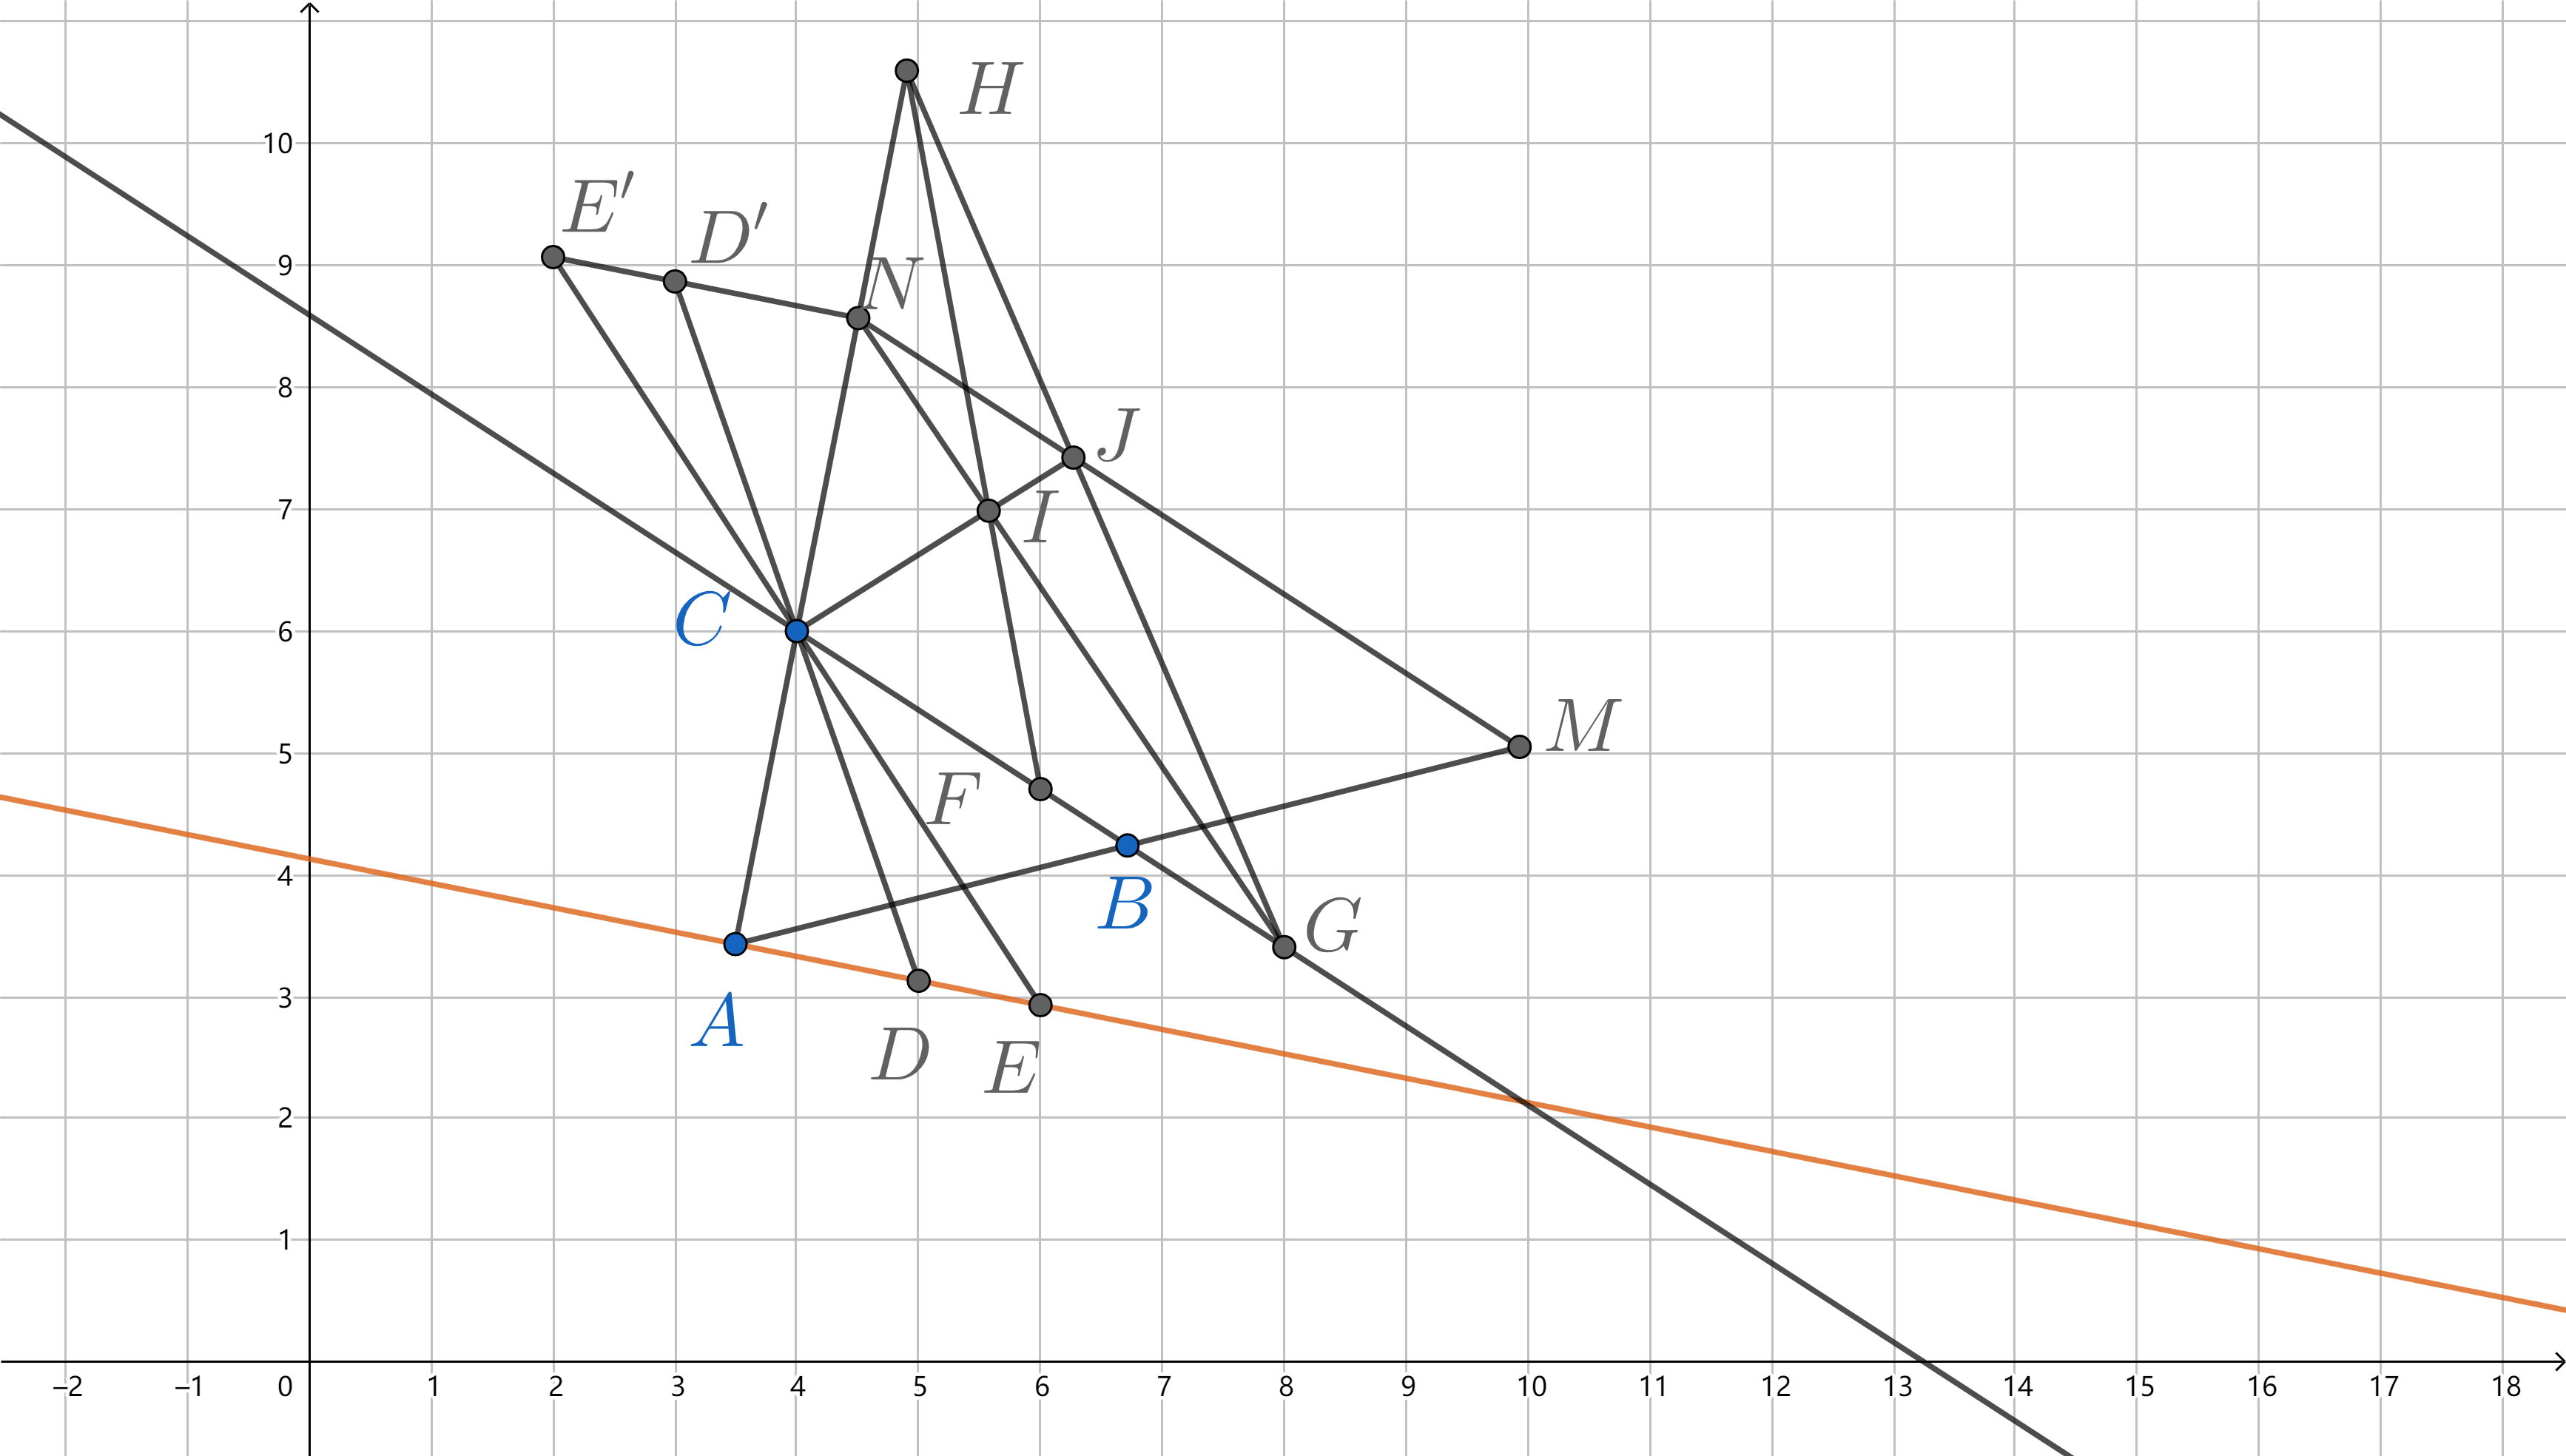
\includegraphics[width=5.76806in,height=3.27292in]{media/image42.png}

如图,\(M\)
即为所求。需要注意的是,广义Wyc倍长线段的图特别容易作乱,画图者需要在倍长线段
\(AC\) 这一步选择合适的点 \(D\) 和点
\(E\)。广义Wyc倍长线段定理显然可以推广至倍长三倍或四倍以及其它的倍数,下面给出了倍长至原线段三倍的图:

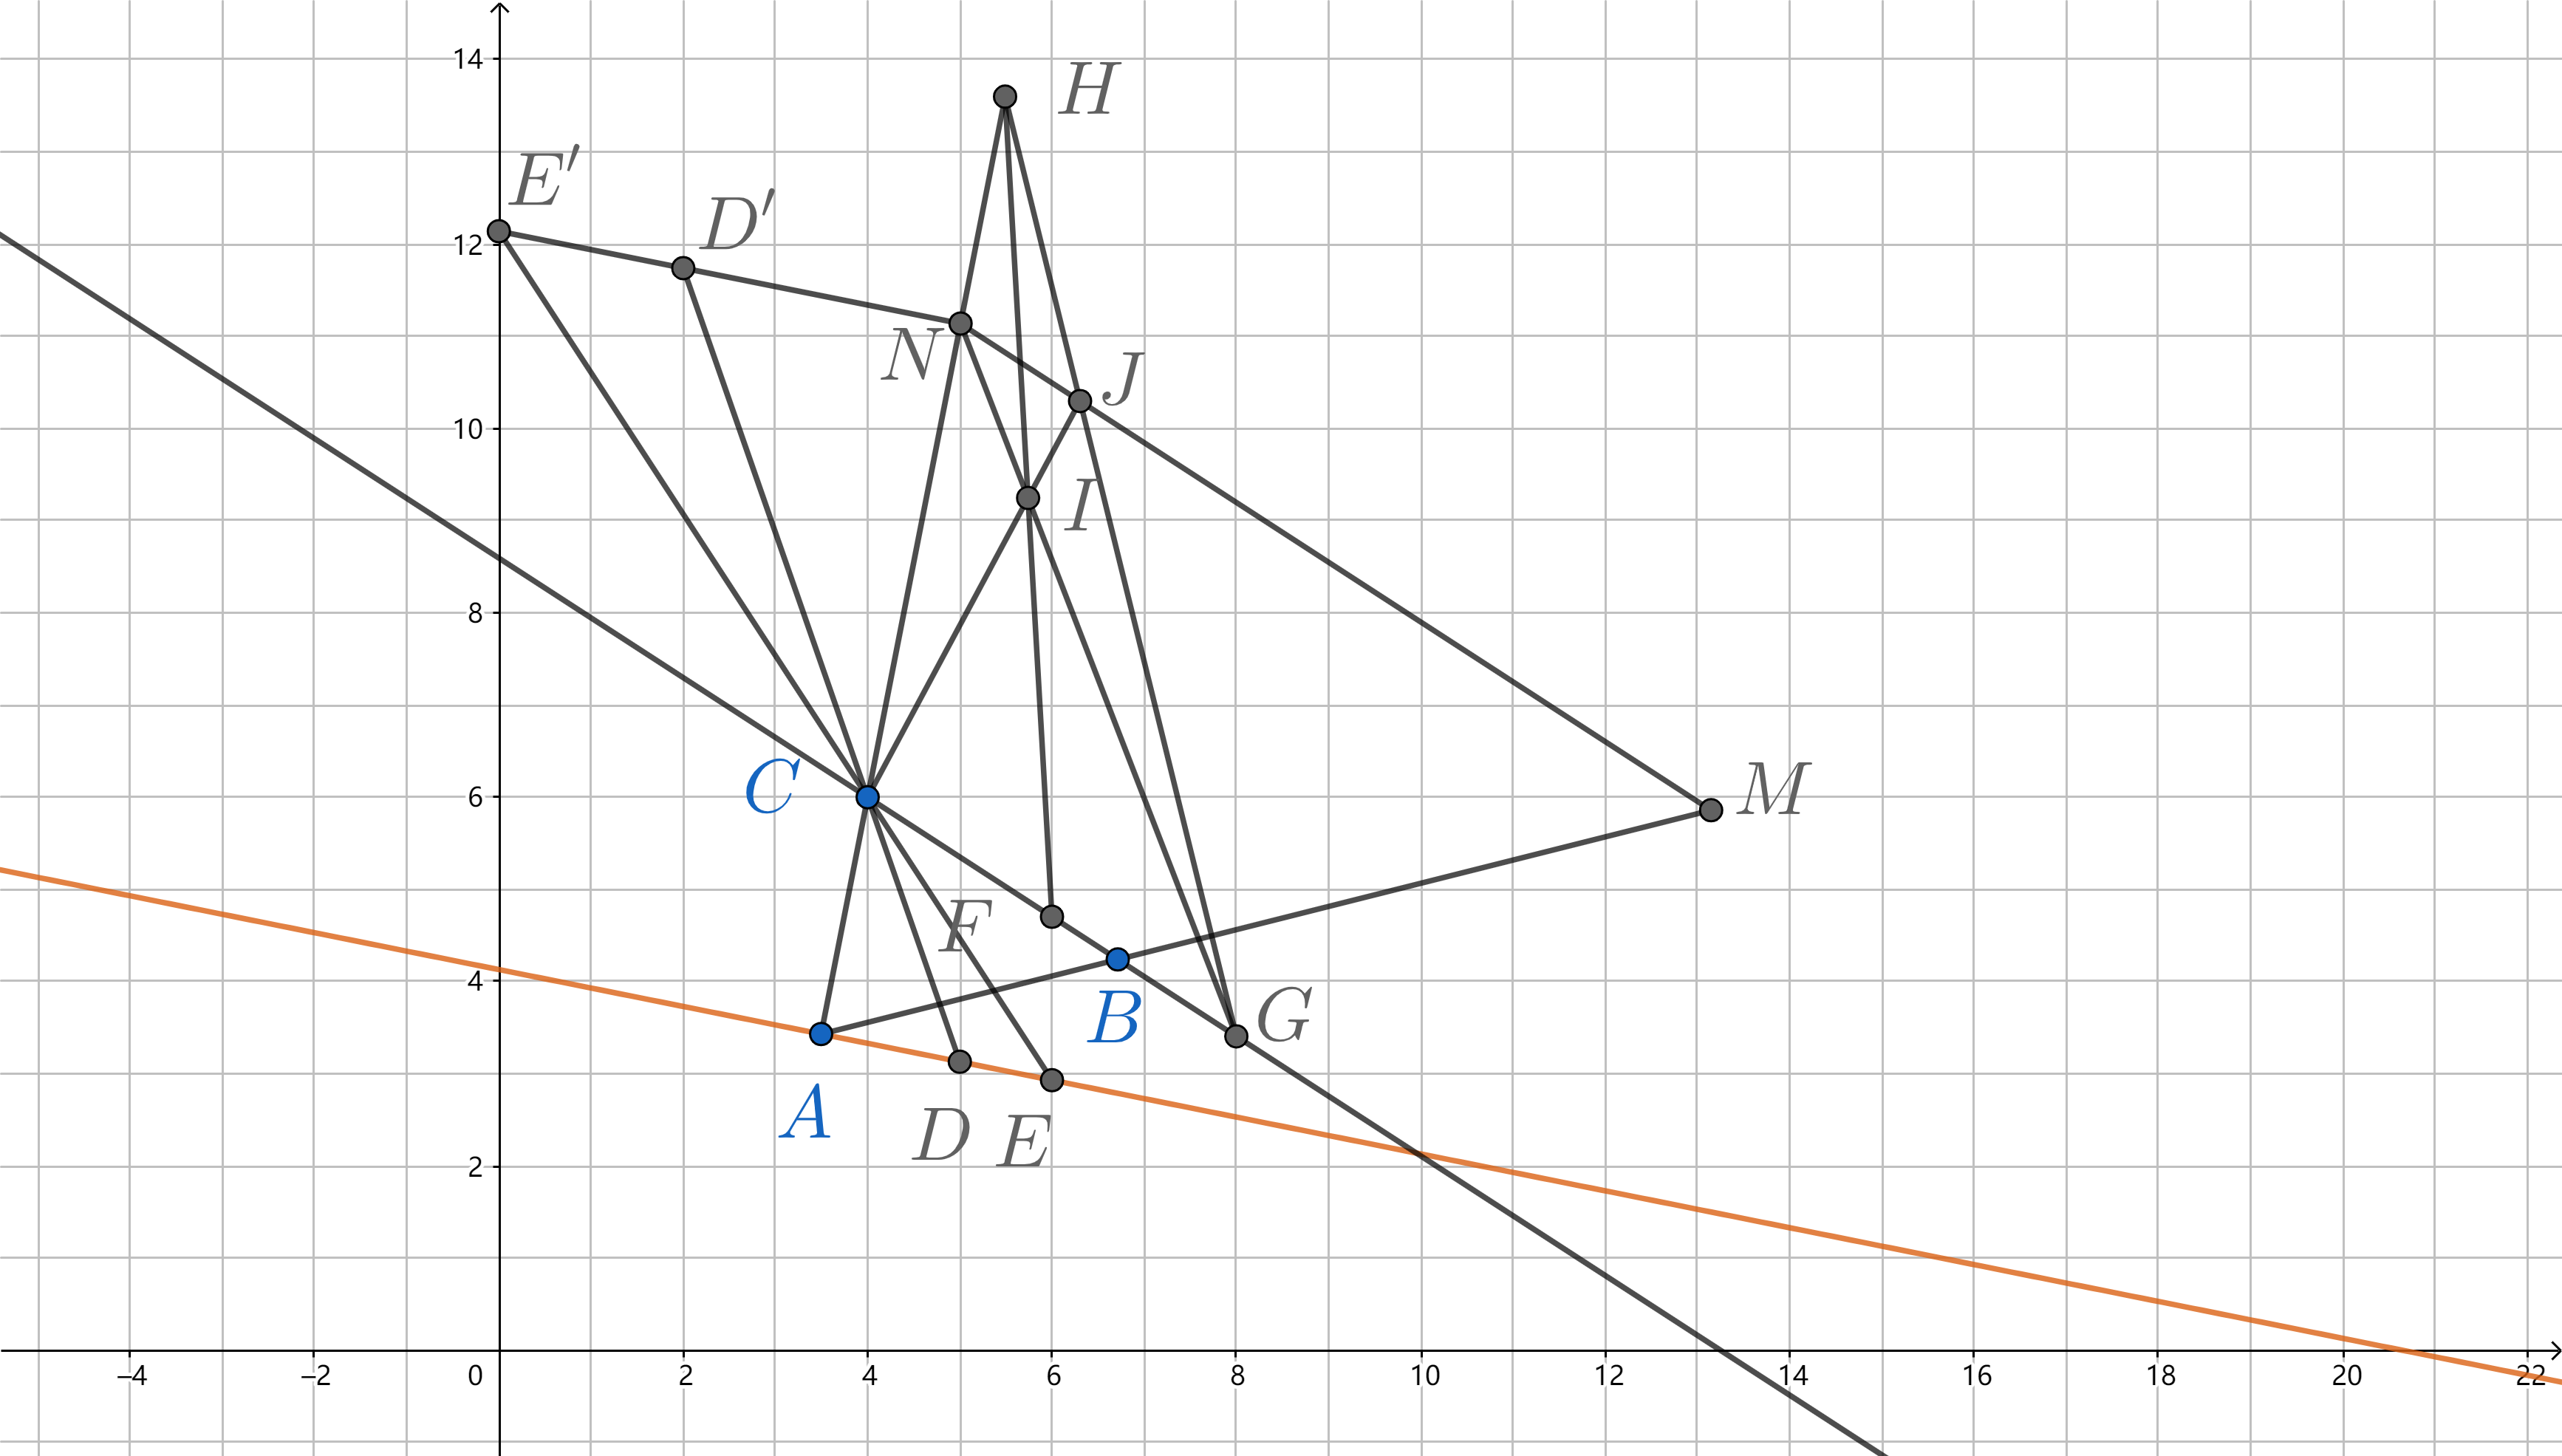
\includegraphics[width=5.76806in,height=3.27847in]{media/image43.png}

\hypertarget{ux5e7fux4e49wycux500dux957fux7ebfux6bb5ux5b9aux7406-wycs-generalized-segment-multiplication-theoremux5b9aux7406-3.7}{%
\subsection{广义Wyc倍长线段定理 Wyc's Generalized Segment Multiplication
Theorem(定理
3.7)}\label{ux5e7fux4e49wycux500dux957fux7ebfux6bb5ux5b9aux7406-wycs-generalized-segment-multiplication-theoremux5b9aux7406-3.7}}

\textbf{【提出者】}翟悦凯(非王宇辰本人提出)

对于任意线段,可以用比倍长线段定理(定理 3.1.3)更简单的方法倍长它。

\subsection{3. 垂直与对称}

\hypertarget{zykux5782ux76f4ux5b9aux7406}{%
\subsubsection{Zyk垂直定理}\label{zykux5782ux76f4ux5b9aux7406}}

Zyk垂直定理解决了过任意格点 \(A\) 任意直线 \(l\) 垂线的问题------但是
\(l\) 必须过 \(A\)。如图:

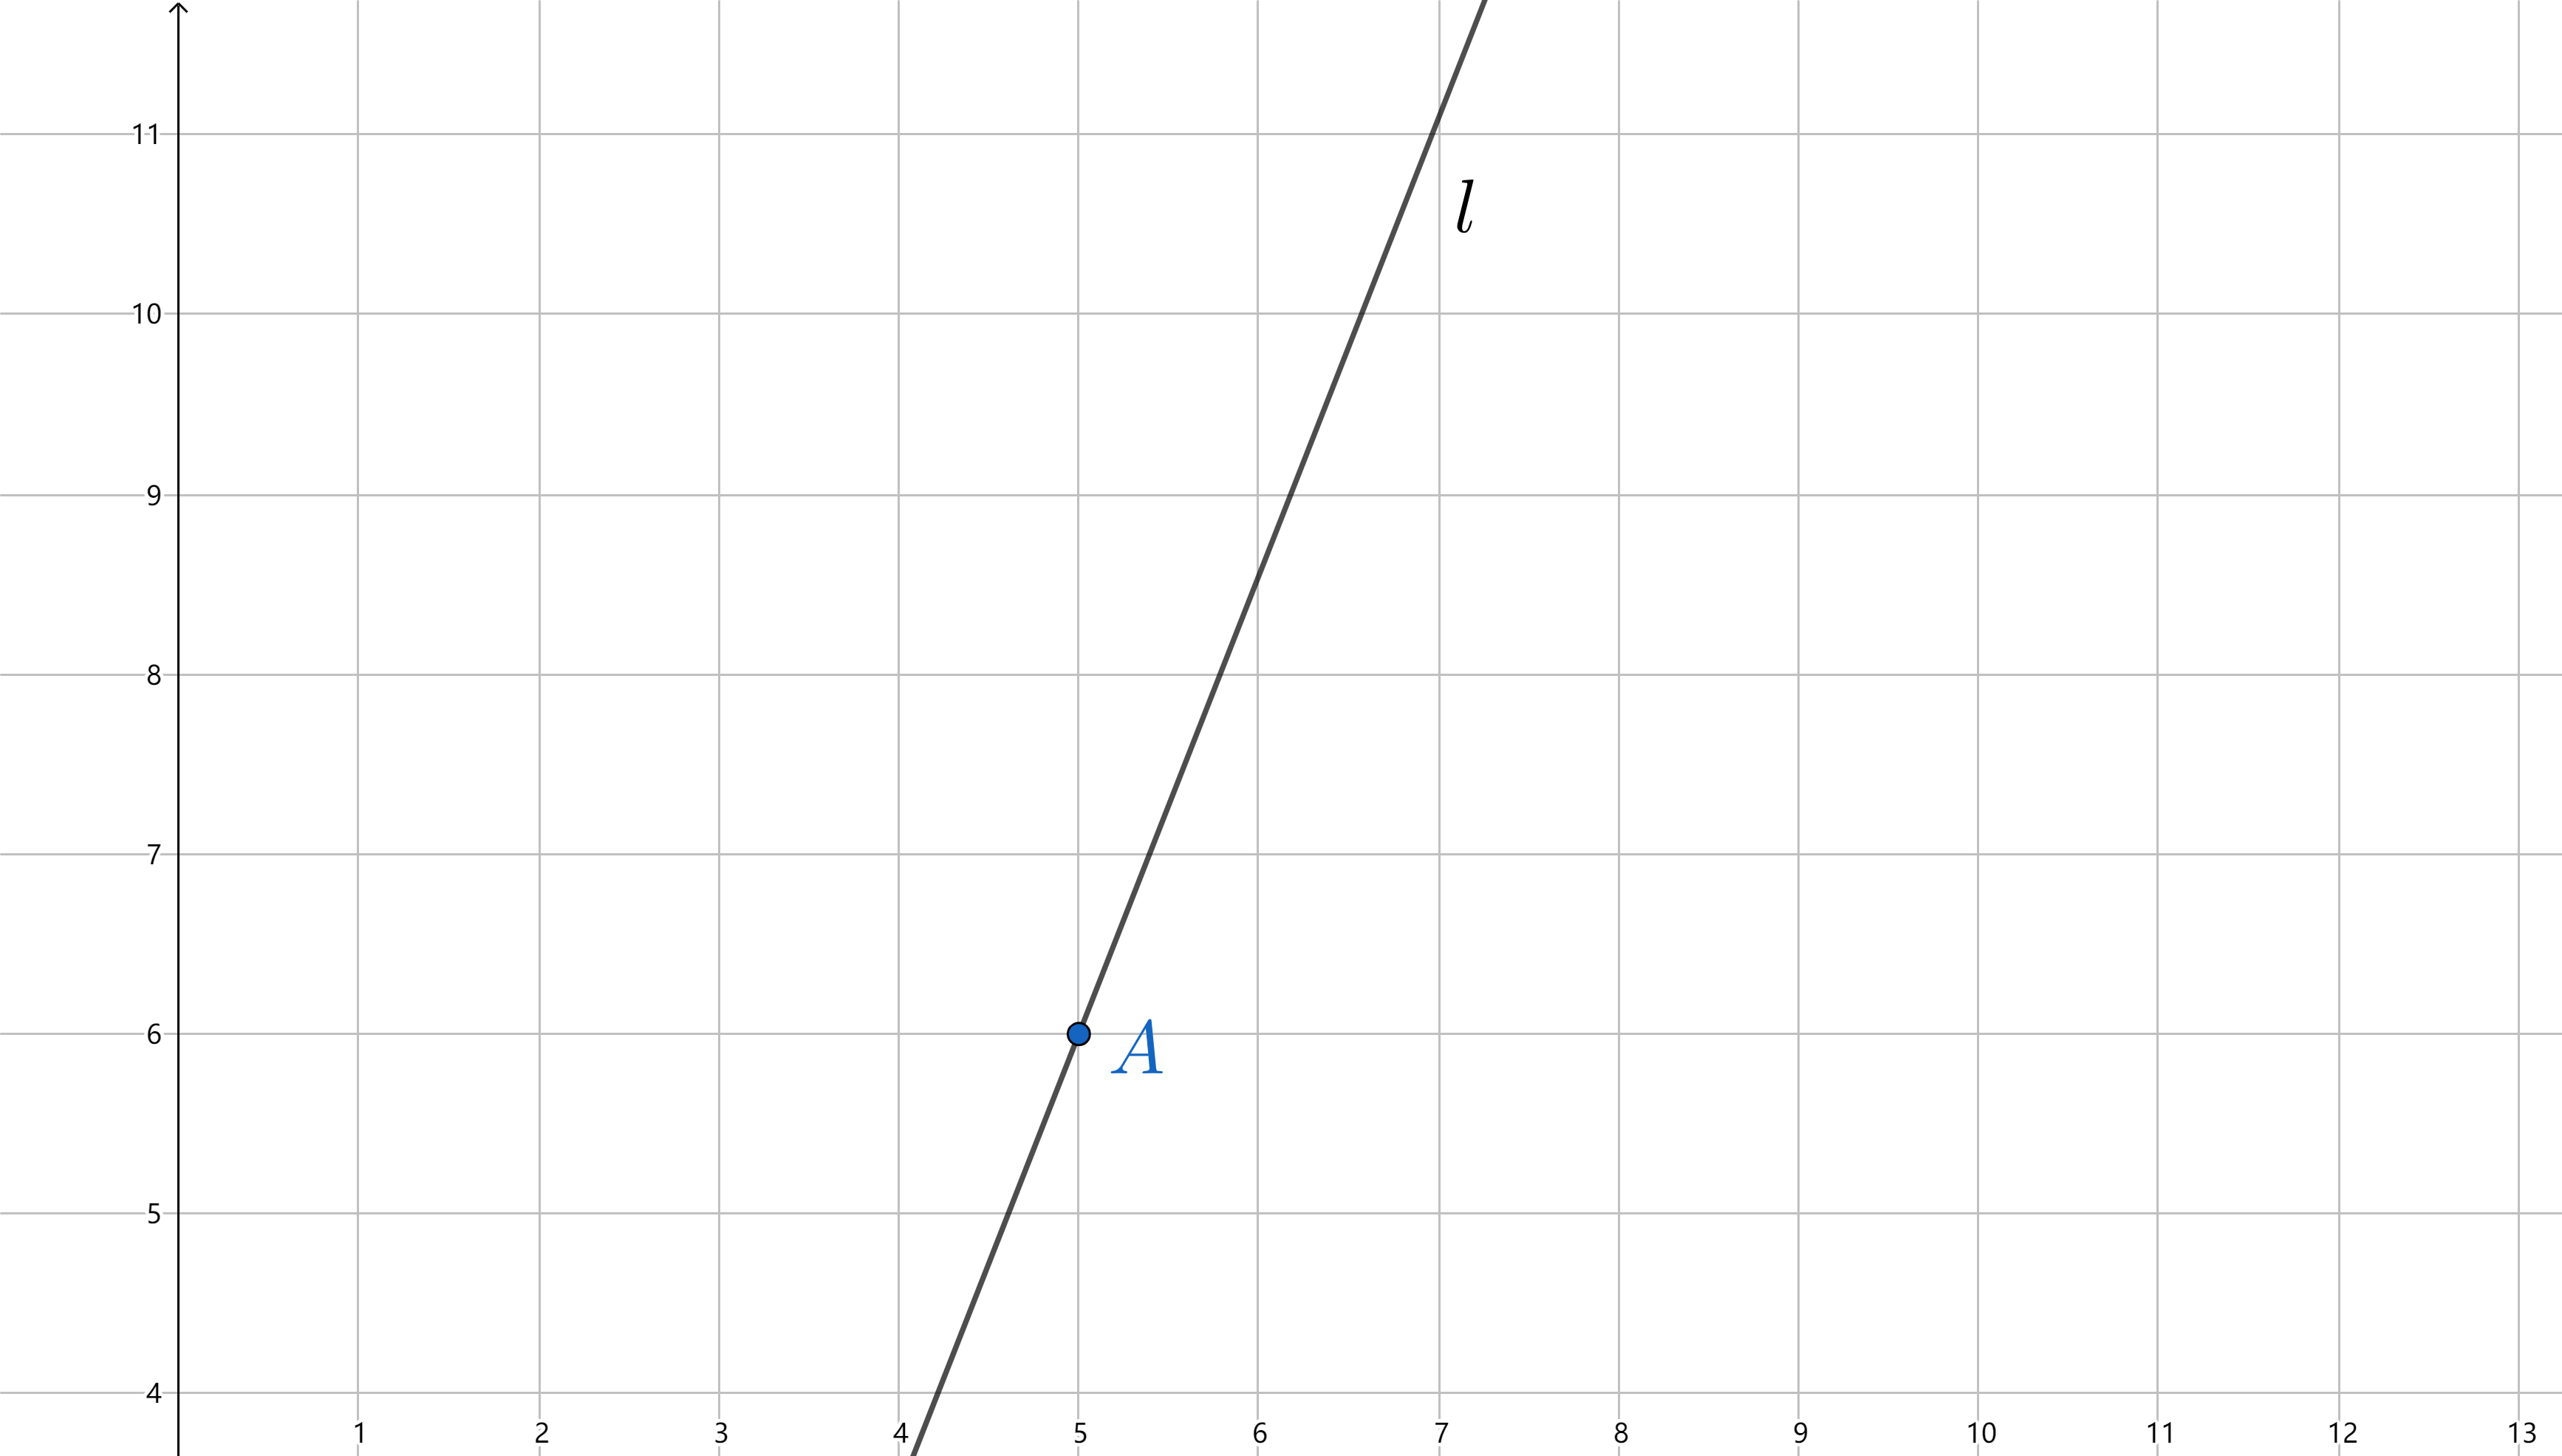
\includegraphics[width=5.76806in,height=3.27847in]{media/image44.png}

如图,\(l\) 过 \(A\),\(A\) 是格点。请过 \(A\) 作 \(l_{2}\bot l\)。

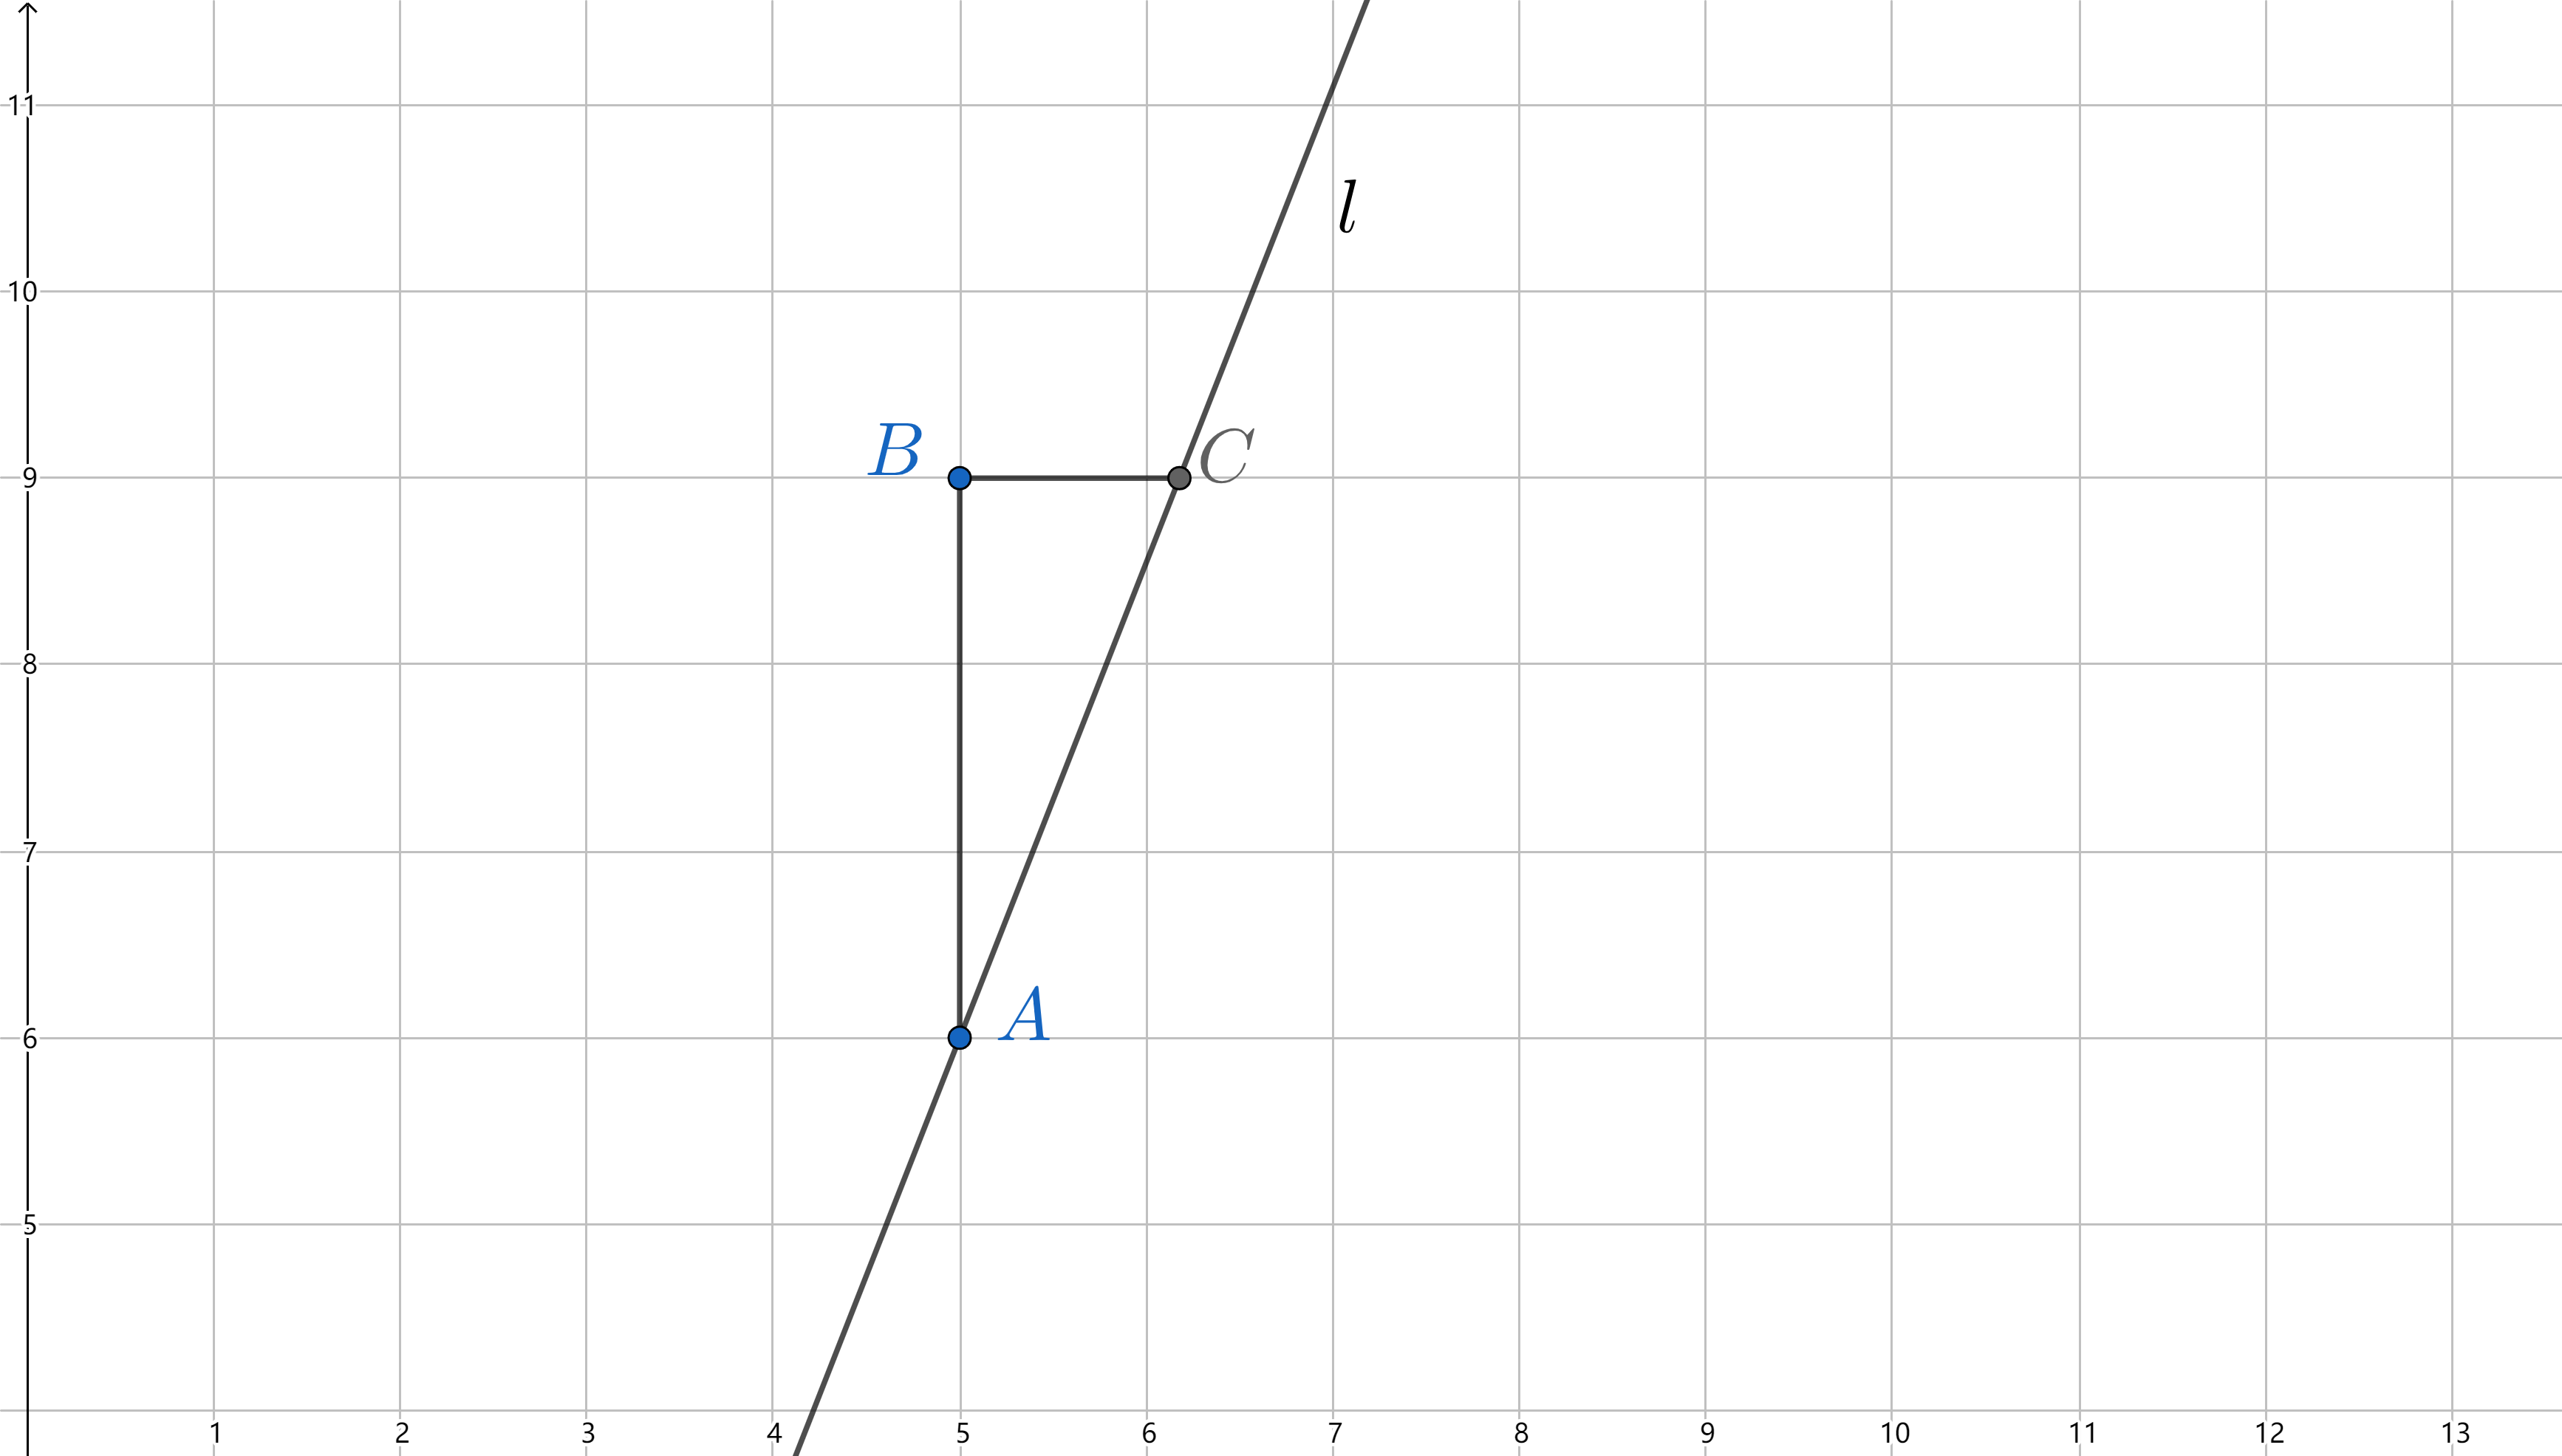
\includegraphics[width=5.76806in,height=3.27847in]{media/image45.png}

如图,我们取格点 \(B\) 和直线与水平格线的交点 \(C\)。如果我们可以把
\(\bigtriangleup ABC\) 逆时针旋转
\(90{^\circ}\),问题就可以得到解决。我们具体这样做:

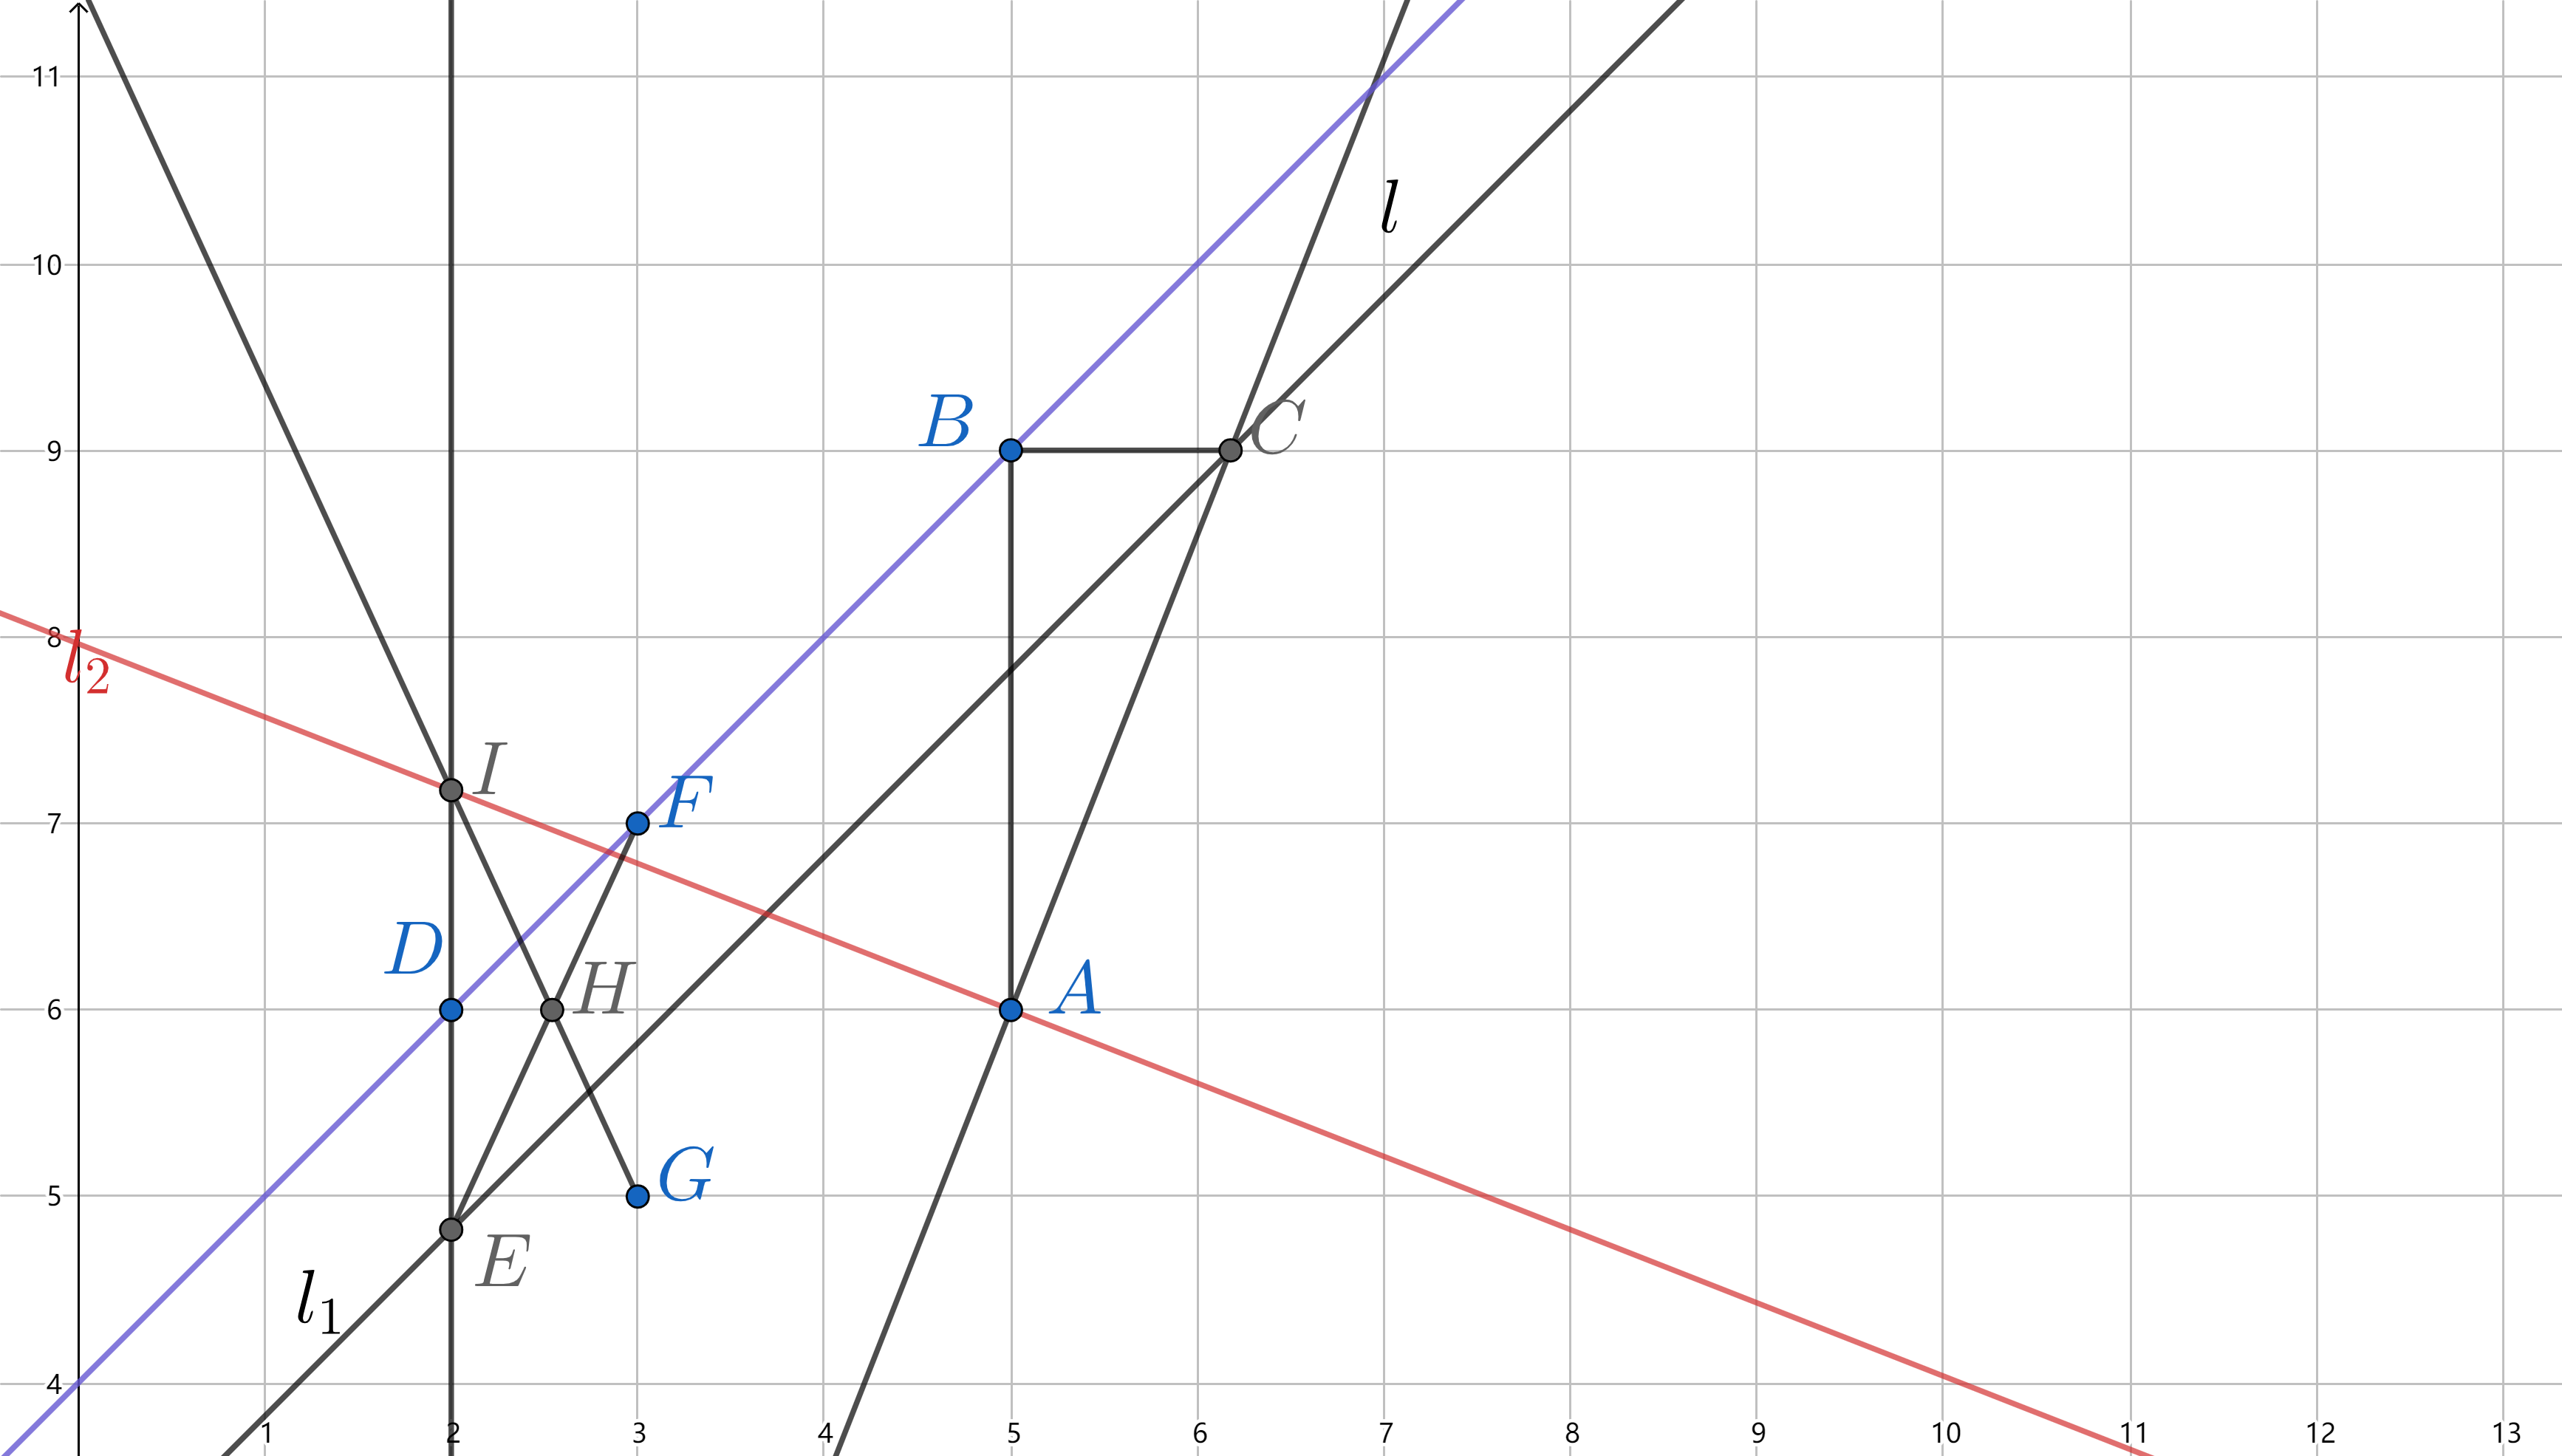
\includegraphics[width=5.76806in,height=3.27847in]{media/image46.png}

去格点 \(D\),连接 \(BD\)。过 \(C\) 作 \(l_{1} \parallel BD\) 交 \(D\)
所在的竖直格线于 \(E\)。作 \(E\) 关于 \(D\) 所在水平格线的对称点
\(I\),连接 \(AI\),\(AI\) 即为所求。

\hypertarget{zykux5782ux76f4ux5b9aux7406-zyks-vertical-theoremux5b9aux7406-3.8}{%
\subsection{Zyk垂直定理 Zyk's Vertical Theorem(定理
3.8)}\label{zykux5782ux76f4ux5b9aux7406-zyks-vertical-theoremux5b9aux7406-3.8}}

\textbf{【提出者】}翟悦凯

如果一直线过一格点,那么我们可以过这个格点作这条直线的垂线。

\hypertarget{hmyux5782ux76f4ux5b9aux7406}{%
\subsubsection{Hmy垂直定理}\label{hmyux5782ux76f4ux5b9aux7406}}

Hmy垂直定理解决了过任意格点 \(A\) 任意直线 \(l\) 垂线的问题------但是
\(l\) 必须过格点 \(A\) (和Zyk垂直定理的情况相同,但是做法更加简单)。

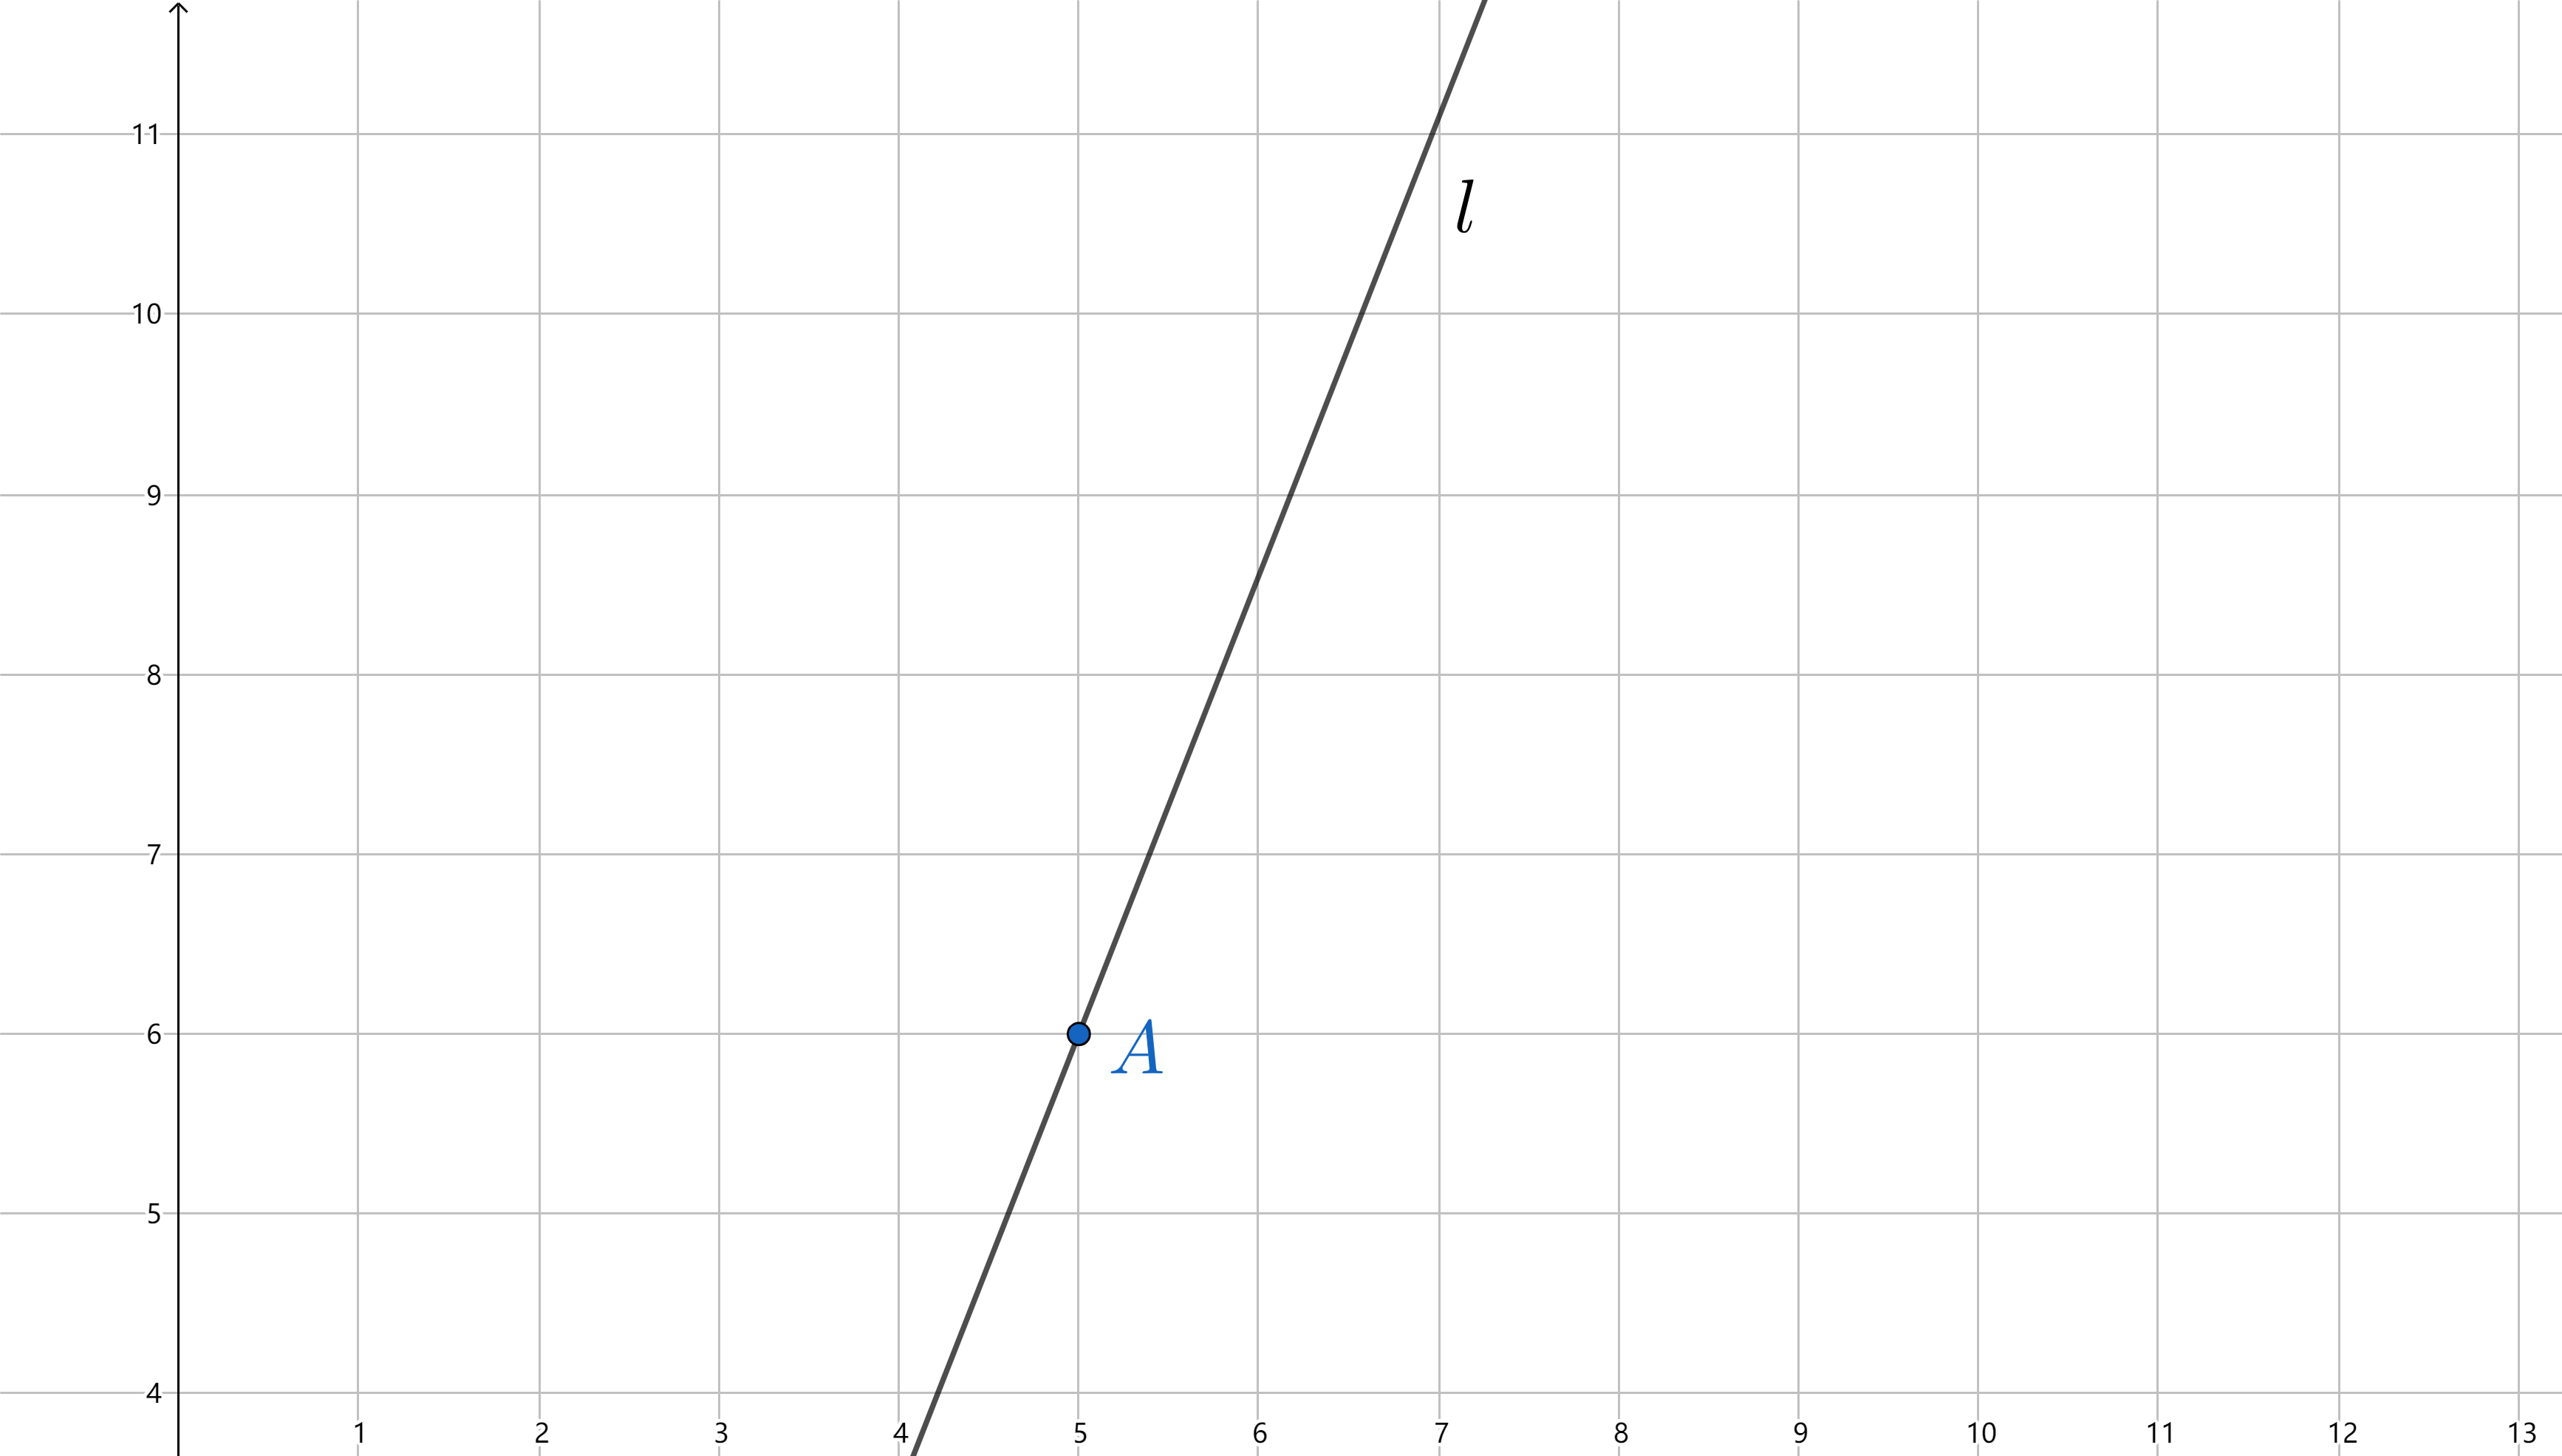
\includegraphics[width=5.76806in,height=3.27847in]{media/image44.png}

如图,\(l\) 过 \(A\),\(A\) 是格点。请过 \(A\) 作 \(l_{2}\bot l\)。

在Zyk垂直定理(定理 3.8)中,我们通过平行+对称的方式得到了 \(C\)
逆时针旋转 \(90{^\circ}\)
后的点;而在这里我们可以通过两个对称的方法得到它。先做 \(C\)
关于网格对角线的对称点 \(G\),再作 \(G\) 关于水平格线的对称点
\(G^{'}\)。

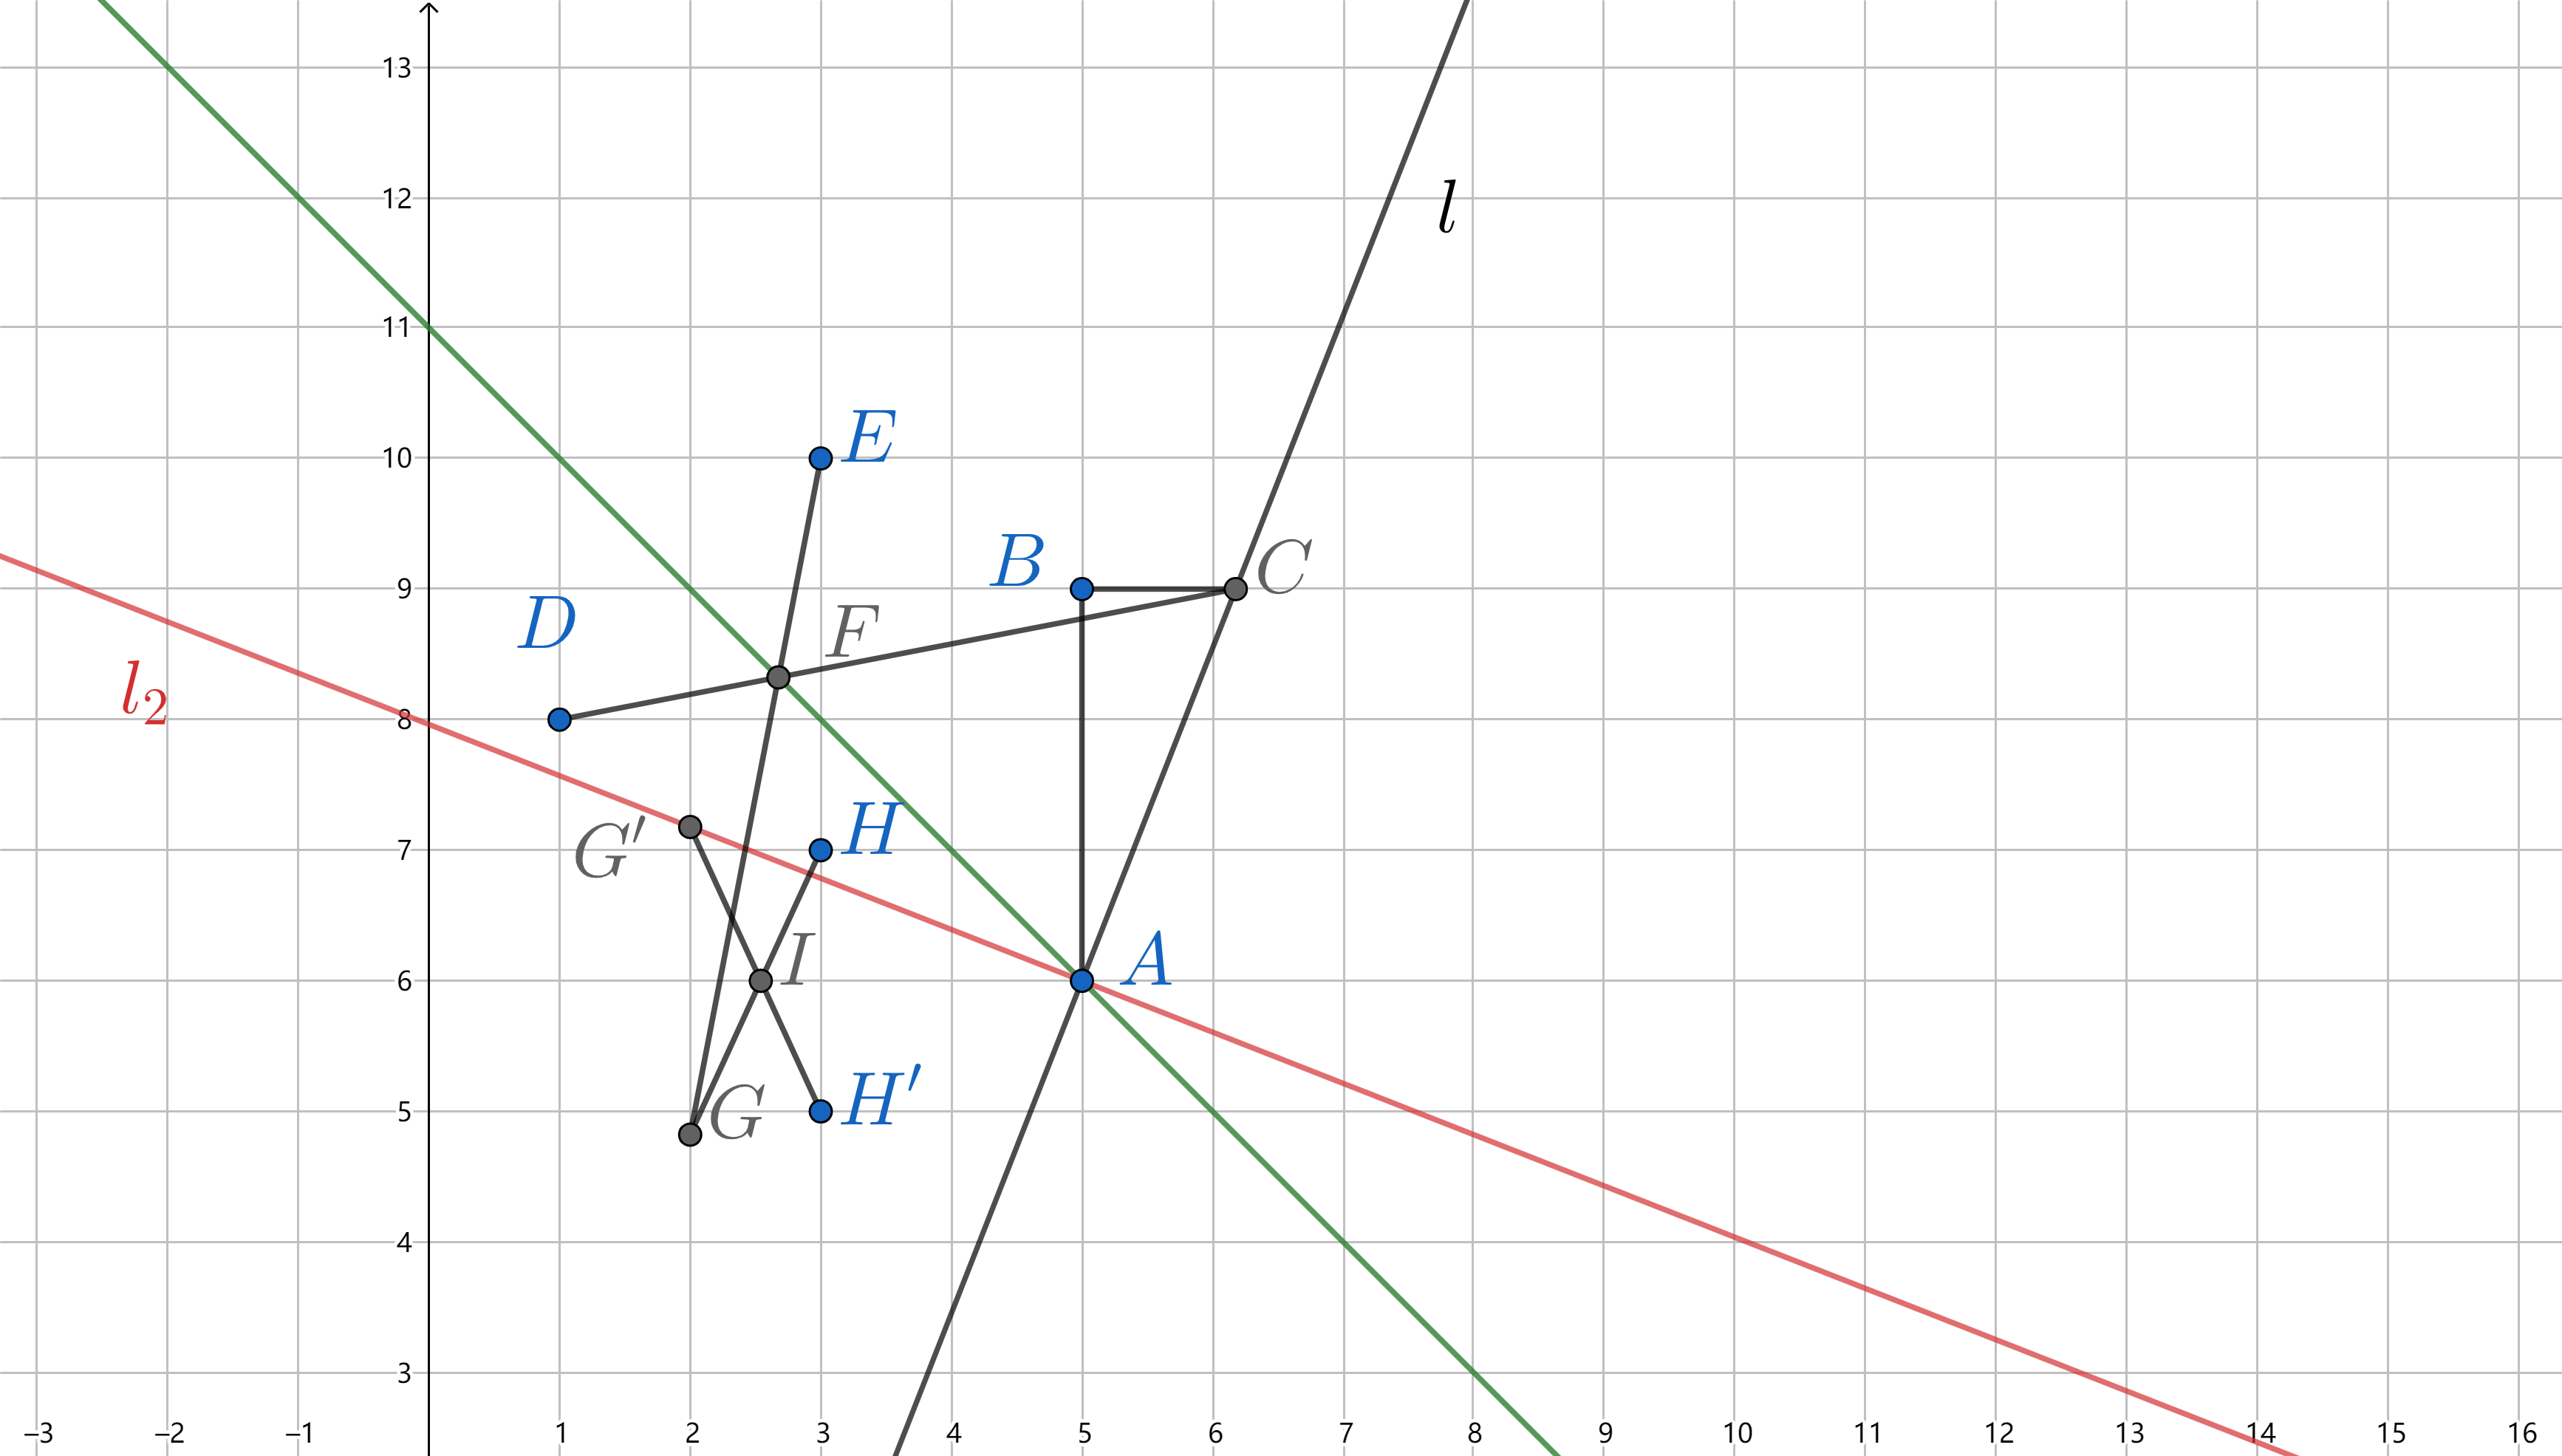
\includegraphics[width=5.76806in,height=3.27847in]{media/image47.png}

\hypertarget{hmyux5782ux76f4ux5b9aux7406-hmys-vertical-theoremux5b9aux7406-3.9}{%
\subsection{Hmy垂直定理 Hmy's Vertical Theorem(定理
3.9)}\label{hmyux5782ux76f4ux5b9aux7406-hmys-vertical-theoremux5b9aux7406-3.9}}

\textbf{【提出者】}郝铭扬

如果一直线过一格点,那么我们可以过这个格点作这条直线的垂线。

\hypertarget{osyux5782ux76f4ux5b9aux7406}{%
\subsubsection{Osy垂直定理}\label{osyux5782ux76f4ux5b9aux7406}}

Osy垂直定理解决了过任意格点作任意直线垂线的问题。我们来看一下图:

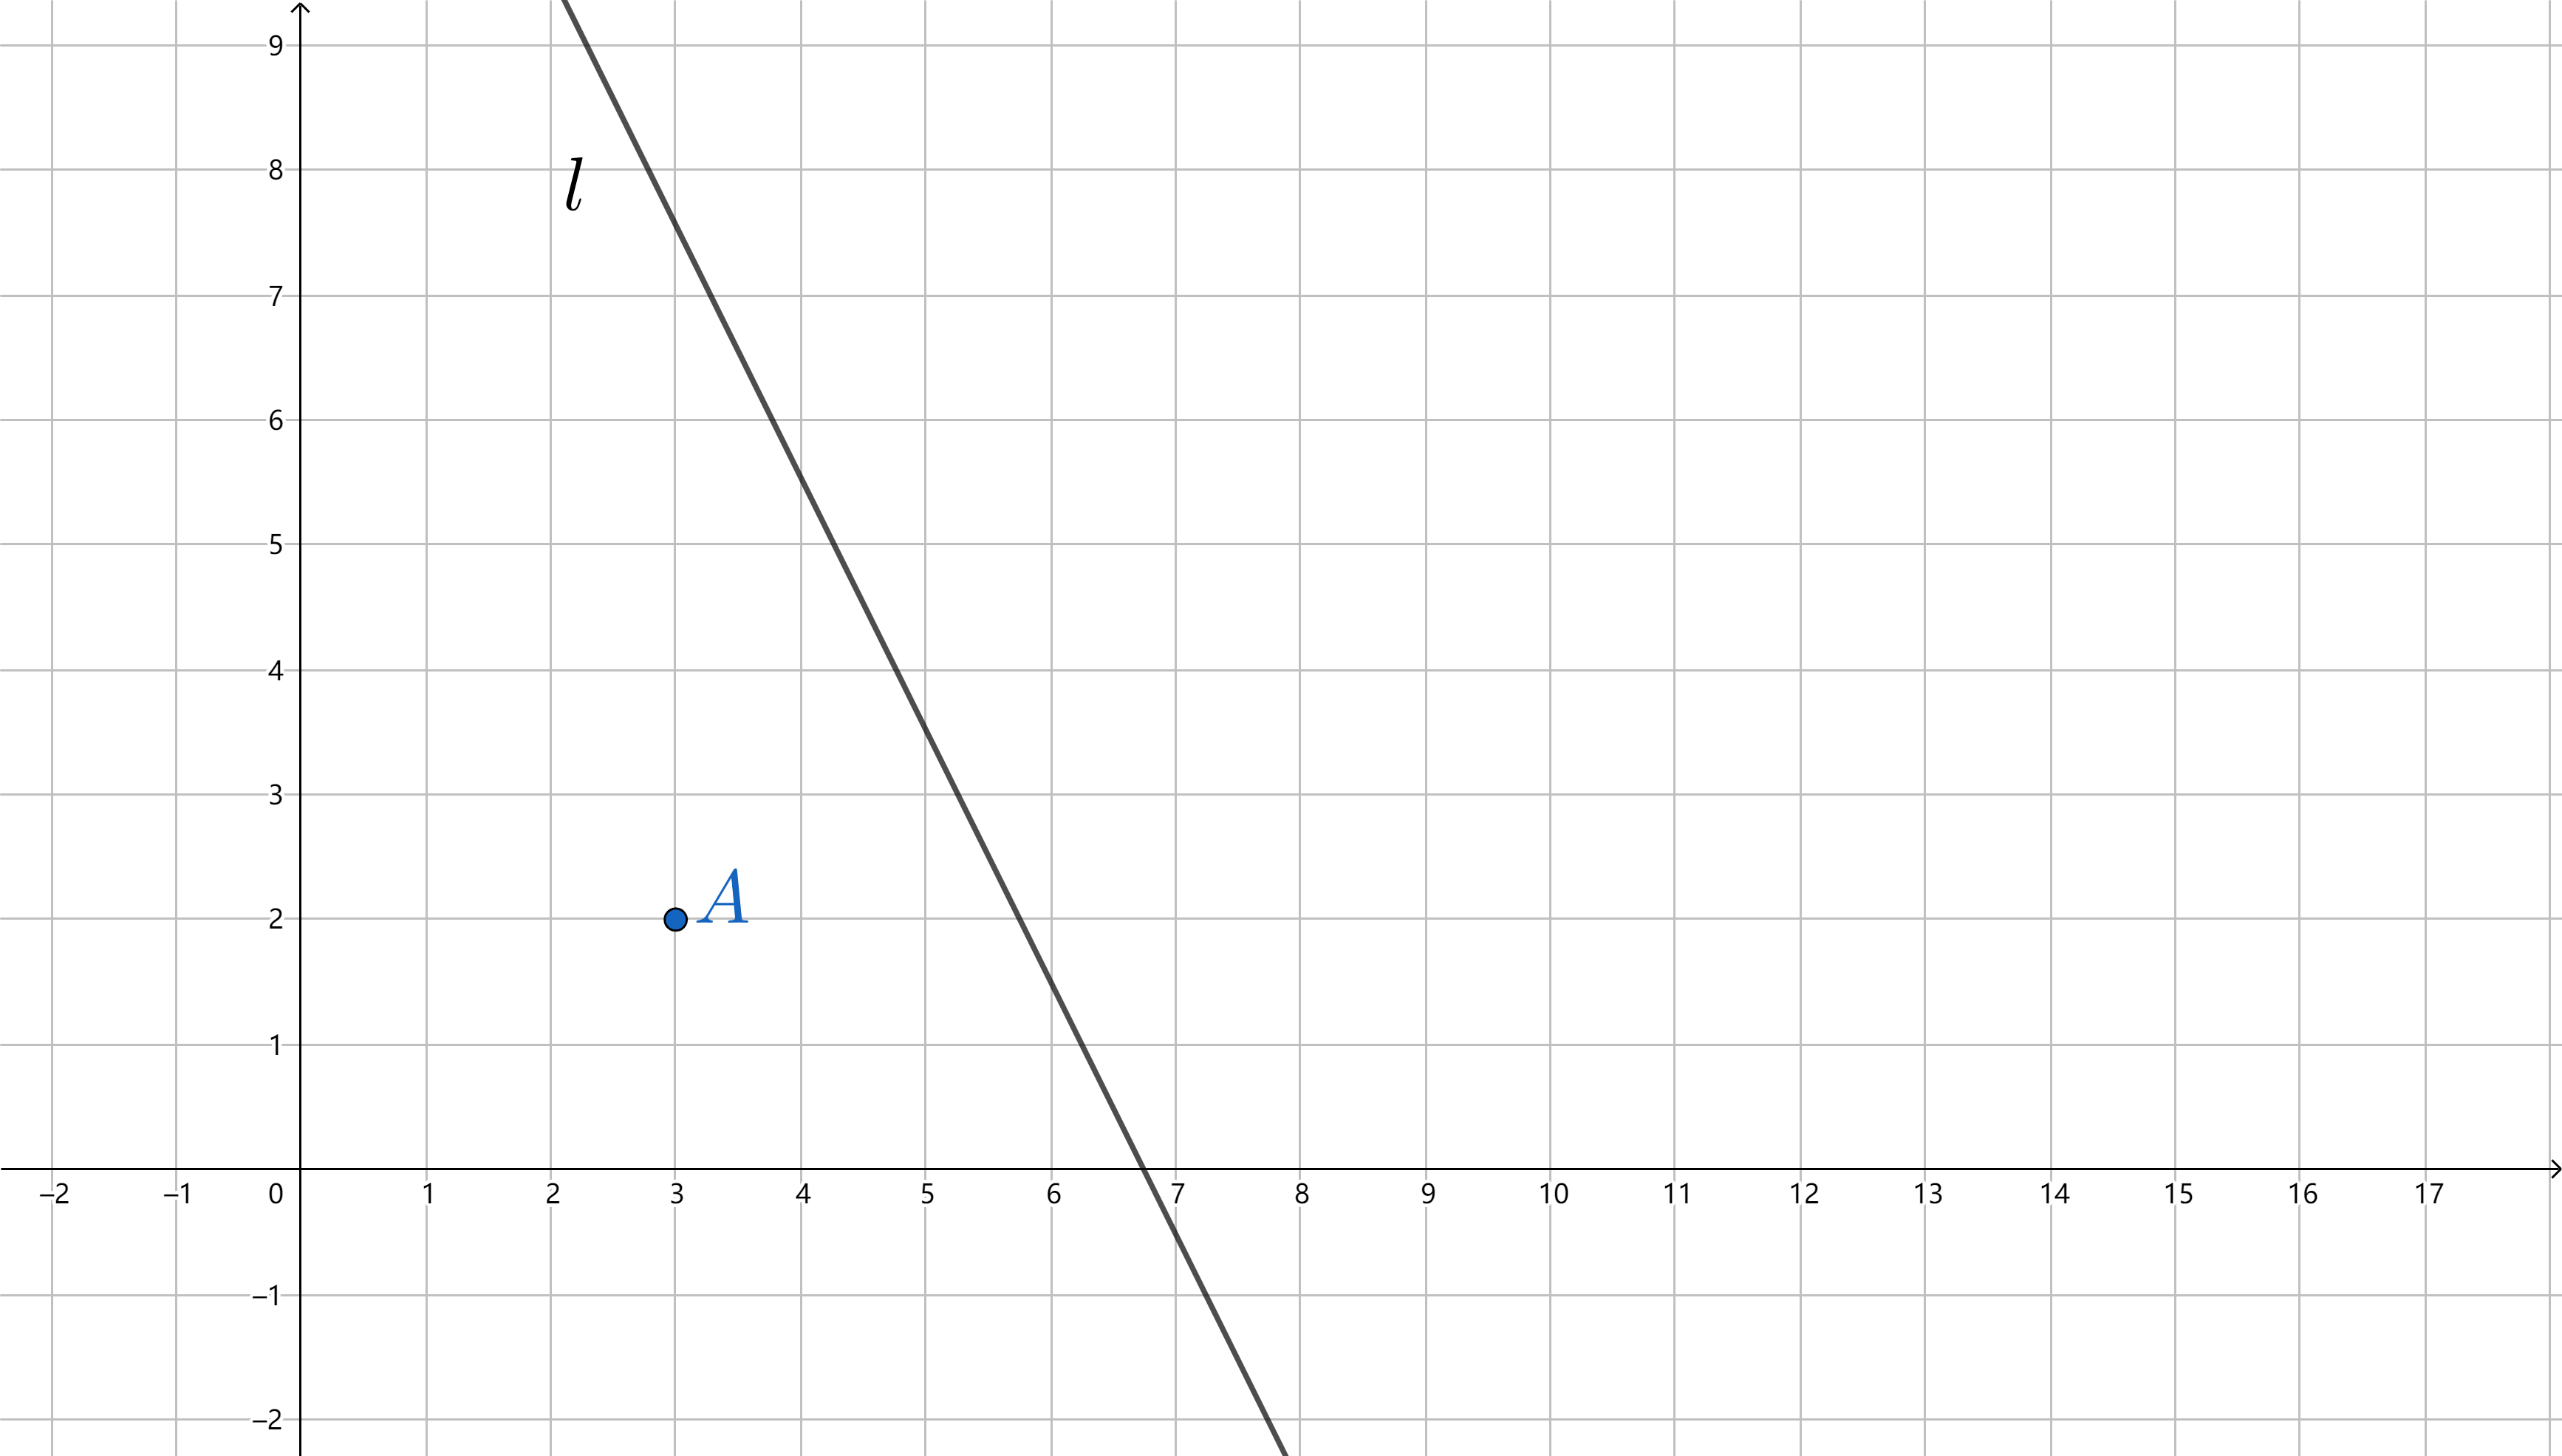
\includegraphics[width=5.76806in,height=3.27847in]{media/image48.png}

如图,\(A\) 是格点,\(l\) 是任意直线,请作 \(l_{2}\bot l\)。

在开始解决这个问题之前,我们先介绍一个几何定理:婆罗摩笈多定理。

\hypertarget{ux5a46ux7f57ux6469ux7b08ux591aux5b9aux7406-ux5b9aux7406-3.10.1}{%
\subsection{婆罗摩笈多定理 (定理
3.10.1)}\label{ux5a46ux7f57ux6469ux7b08ux591aux5b9aux7406-ux5b9aux7406-3.10.1}}

\includegraphics[width=5.76806in,height=3.27847in]{media/image49.png}

\(CD\),\(AB\) 是两条相交且垂直的弦,\(M\) 是 \(BD\) 中点,连接 \(ME\)
并延长交 \(AC\) 于 \(N\),则有 \(MN\bot AC\)。

\textbf{【证明】}因为
\(\overset{\frown}{BC} = \overset{\frown}{BC}\),所以
\(\angle A = \angle D\)。因为 \(M\) 是 \(BD\)
的中点,\(\angle BED = 90{^\circ}\),所以
\(MD = ME = MB\),\(\angle D = \angle MED = \angle CEN\)。所以
\(\angle CNE = 90{^\circ}\),\(MN\bot AC\)。

婆罗摩笈多定理可以将垂直转化为中点,而我们又有很多的方法和定理作中点,所以我们可以考虑使用婆罗摩笈多定理解决这个问题。我们先将
\(l\) 于过 \(A\) 的竖直和水平格线分别交于 \(B\),\(C\)。

\includegraphics[width=5.76806in,height=3.27847in]{media/image50.png}

我们可以过 \(A\) 做一条网格的对角线(即下图 \(l_{1}\)),并将
\(\bigtriangleup ABC\)
翻折过去,这样就可以得到一个圆内接四边形(如下图)。因为翻折,所以
\(\angle B^{'}C^{'}B = \angle B^{'}CB\),这符合同弧所对圆周角相等的定理,所以
\(B\),\(C\),\(C^{'}\),\(B^{'}\) 是四点共圆的。

\includegraphics[width=5.76806in,height=3.27847in]{media/image51.png}

要做出 \(B\),\(C\) 关于 \(l_{1}\)
的对称点并不难。首先它们肯定在水平或竖直格线上,而我们可以推广Zyk基本对称定理来解决这个问题。

\includegraphics[width=5.76806in,height=3.27847in]{media/image52.png}

如图,我选了两组对称点(\(D\) 和 \(D^{'}\),\(F\) 和 \(F^{'}\))做出了
\(B\) 和 \(C\) 的对称点 \(B^{'}\) 和 \(C^{'}\)。我们现在只需做出线段
\(B^{'}C^{'}\) 的中点 \(N\),再连接 \(NA\) 并延长交 \(BC\) 于
\(M\),连接 \(AM\),\(AM\) 即为所求。做出 \(B^{'}C^{'}\)
的中点,我们可以使用Wyc分线段定理,但是这里我们也可以直接使用朴素平移定理。

\includegraphics[width=5.76806in,height=3.27847in]{media/image53.png}

如图,我将 \(B^{'}\) 向下平移了两个单位,将 \(C^{'}\)
向上平移了两个单位。

\textbf{【拓展】}\(A\) 关于 \(l\)
的对称点也可以通过这个方法做出来------倍长 \(AM\)
即可。下面是我给出的作图。

\includegraphics[width=5.76806in,height=3.27847in]{media/image54.png}

\hypertarget{osyux5782ux76f4ux5b9aux7406-osys-vertical-theoremux5b9aux7406-3.10}{%
\subsection{Osy垂直定理 Osy's Vertical Theorem(定理
3.10)}\label{osyux5782ux76f4ux5b9aux7406-osys-vertical-theoremux5b9aux7406-3.10}}

\textbf{【提出者】}欧思远

可以过任意一格点作任意一条直线的垂线,也可以作这个格点关于这条直线的对称点。

\hypertarget{ux4efbux610fux5782ux76f4ux548cux4efbux610fux5bf9ux79f0}{%
\subsubsection{任意垂直和任意对称}\label{ux4efbux610fux5782ux76f4ux548cux4efbux610fux5bf9ux79f0}}

有了这两个定理,我们就可以过任意点作任意直线的垂线了。

\hypertarget{ux4efbux610fux5782ux76f4ux5b9aux7406-arbitrary-vertical-theoremux5b9aux7406-3.11}{%
\subsection{任意垂直定理 Arbitrary Vertical Theorem(定理
3.11)}\label{ux4efbux610fux5782ux76f4ux5b9aux7406-arbitrary-vertical-theoremux5b9aux7406-3.11}}

\includegraphics[width=5.76806in,height=3.27847in]{media/image55.png}

可以过任意一点 \(A\) 作任意一条直线 \(l\) 的垂线。我们有两种做法:

\textbf{做法 1:利用Zyk垂直定理(定理 3.8)或Hmy垂直定理(定理 3.9)}

\includegraphics[width=5.76806in,height=3.27847in]{media/image56.png}

如图,选择格点 \(B\),过 \(B\) 作
\(l_{1} \parallel l\),利用Zyk垂直定理(定理 3.8)或Hmy垂直定理(定理
3.9)过 \(B\) 作 \(l_{2}\bot l_{1}\),过 \(A\) 作
\(l_{3} \parallel l_{2}\),\(l_{3}\) 即为所求。

\textbf{做法 2:利用Osy垂直定理(定理 3.10)}

\includegraphics[width=5.76806in,height=3.27847in]{media/image57.png}

如图,选择格点 \(B\),利用Osy垂直定理(定理 3.10)过 \(B\) 作
\(l_{2}\bot l\),过 \(A\) 作 \(l_{3} \parallel l_{2}\),\(l_{3}\)
即为所求。

我们甚至可以作任意点关于任意直线的对称点。

\hypertarget{ux4efbux610fux5bf9ux79f0ux5b9aux7406-arbitrary-symmetry-theoremux5b9aux7406-3.12}{%
\subsection{任意对称定理 Arbitrary Symmetry Theorem(定理
3.12)}\label{ux4efbux610fux5bf9ux79f0ux5b9aux7406-arbitrary-symmetry-theoremux5b9aux7406-3.12}}

\textbf{【提出者】}郝铭扬

可以作任意点关于任意直线的对称点。作图如下:

\includegraphics[width=5.76806in,height=3.27847in]{media/image58.png}

如图,在直线的另一侧选取合适的格点 \(B\),利用Osy垂直定理(定理
3.10)的拓展做出 \(B\) 关于 \(l\) 的对称点 \(B^{'}\),连 \(B^{'}A\)
并延长交 \(l\) 于 \(C\),连 \(BC\)。连 \(AB\) 交 \(l\) 于 \(D\),连
\(B^{'}D\) 并延长交 \(BC\) 于 \(A^{'}\)。\(A^{'}\) 即为所求。

我们来用Osy垂直定理的最后一张图来演示一下任意对称定理:

\includegraphics[width=5.76806in,height=3.27847in]{media/image59.png}

可以看到,在这张图中,我们成功地做出了任意点 \(P\) 关于任意直线 \(l\)
的对称点。

\end{document}
